\documentclass[
  11pt,             % 10pt | 11pt | 12pt
  french,           % french | english
  greyCover,        %
  fancyChapter,     %
  fancyPart,        %
  squeezeCommittee, %
  %showframe         %
]{these-LUNAM_mod}

% TODO utiliser subcaption plutot que subfigure
%\usepackage{etex}                             % solve compatibility issues
\usepackage[utf8]{inputenc}                   %
\usepackage[T1]{fontenc}                      %
\usepackage{textcomp}                         % °, <<, >>, etc.
\usepackage{times}                            %
\usepackage{natbib}                           %
\usepackage{xifthen}                          %
\usepackage{relsize}                          % \mathlarger
\usepackage{multirow}                         %
\usepackage{booktabs}                         % \addlinespace, \toprule, etc.
\usepackage{subfigure}                        %
\usepackage{tikz}                             %
\usepackage{pgfplots}                         %
\usepackage{makeidx}                          %
\usepackage{amsthm}                           % theorem definition and styling
\usepackage{epigraph}                         % chapter heading quote
\usepackage[inline]{enumitem}                 %
\usepackage{ragged2e}                         % \justifying
\usepackage{rotating}                         % \sideways in table
\usepackage{lipsum}                           %
\usepackage{mathabx}                          % $\drsh$
\usepackage[ruled,linesnumbered]{algorithm2e} %
\usepackage{listings}                         %
\usepackage{units}                            % \unitfrac
\usepackage{overpic}                          %
\usepackage{fancyhdr}

\usetikzlibrary{positioning, topaths, shapes, arrows, patterns, calc}

\setlength\epigraphwidth{10cm}
\setlength\epigraphrule{0cm}

\RequirePackage[bookmarks,
                colorlinks,
                urlcolor=black,
                citecolor=black,
                linkcolor=black,
                hyperfigures,
                pagebackref,
                pdfcreator=LaTeX,
                breaklinks=true,
                pdfpagelayout=SinglePage,
                bookmarksopen=true,
                bookmarksopenlevel=2]{hyperref}

\geometry{inner=2.5cm, outer=2.5cm, top=2.5cm, bottom=2cm}
\geometry{inner=3.5cm, outer=3.5cm, top=4cm, bottom=3.5cm} % CUSTOM
%\geometry{inner=1.5cm, outer=1.5cm, top=2cm, bottom=2cm}
%%%%%%%%%%%%%%%%%%%%%%%%%%%%%%%%%%%%%%%%%%%%%%%%%%%%%%%%%%%%%%%%%%%%%%%%%%%%%%%%
\renewcommand{\chaptermark}[1]{\markboth{#1}{}}
\renewcommand{\sectionmark}[1]{\markright{#1}}
\pagestyle{fancy}
\fancyhf{}
\fancyhead[LE]{\thepage\hspace{.5cm}}
\fancyhead[RO]{\hspace{.5cm}\thepage}
\fancyhead[LO]{\itshape\nouppercase{\rightmark}}
\fancyhead[RE]{\itshape\nouppercase{\leftmark}}
\renewcommand{\headrulewidth}{0pt}
%%%%%%%%%%%%%%%%%%%%%%%%%%%%%%%%%%%%%%%%%%%%%%%%%%%%%%%%%%%%%%%%%%%%%%%%%%%%%%%%


\setlist[enumerate]{itemsep=0mm}  % minimum spacing between items (it is not
\setlist[itemize]{itemsep=0mm}    % same as \setlist[...]{noitemsep}
\renewcommand{\labelitemi}{--}
\renewcommand{\labelitemii}{-}
\renewcommand{\labelitemiii}{-}
\renewcommand{\labelitemiv}{-}

%-------------------------------------------------------------------------------

\makeatletter
\newcommand*{\overtabline}{%
  \noalign{%
    % normal "baselineskip" in tabular is height + depth of \@arstrutbox
    \vskip-.5\dimexpr\ht\@arstrutbox+\dp\@arstrutbox\relax
    % default line thickness is 0.4pt
    \vskip-.2pt\relax
    \hrule height .1pt
    \vskip-.2pt\relax
    \vskip+.5\dimexpr\ht\@arstrutbox+\dp\@arstrutbox\relax
  }%
}
\makeatother

%-------------------------------------------------------------------------------
\newcommand\setlstxml{
  \footnotesize
  \lstset{language=XML}
  \lstset{morekeywords={
    notice, titre, resume, encoding, TEI, xmlns, xmlns:tei, teiHeader, fileDesc,
    sourceDesc, biblStruct, type, analytic, title, author, persName, ana,
    forename, surname, profileDesc, abstract, p, martif, martifHeader, text,
    body, termEntry, langSet, tig, term, xml:id, stdf, soHeader, annotations,
    annotationGrp, target, span, from, num, link, note
  }}
  \lstset{literate={'}{{'}}1 {é}{{\'e}}1 {è}{{\`e}}1 {ê}{{\^e}}1 {à}{{\`a}}1 {ô}{{\^o}}1}
  \lstset{frame=single}
  \lstset{stringstyle=\color{red}}
  \lstset{keywordstyle=\color{blue}}
}

%-------------------------------------------------------------------------------

\newcommand\chaptercite[4]{\setlength{\epigraphwidth}{#3}\epigraph{#4{\Large\og{}}#1{\Large\fg{}}}{--- #2}}

\newcommand\ditto{$_{^\textnormal{\normalsize\textquotedbl}}$}

\renewcommand\cite[2][]{\ifthenelse{\equal{#1}{}}{\citep{#2}}{\citep[#1]{#2}}}
\newcommand\newcite[2][]{\ifthenelse{\equal{#1}{}}{\citet{#2}}{\citet[#1]{#2}}}

\newcommand\TODO[1]{\textcolor[rgb]{1, 0, 0}{[TODO #1]}}
\newcommand\REMARK[1]{\textcolor[rgb]{0, 1, 0}{[#1]}}
\newcommand\ANNOTATE[2]{\textcolor{blue}{[#1 \textbf{$\rightarrow$ #2}]}}
\newcommand\FILL[1]{\textcolor{red}{\lipsum[#1]}}

\theoremstyle{remark}
\newtheorem{example}{Exemple}

\makeindex

%%%%%%%%%%%%%%%%%%%%%%%%%%%%%%%%%%%%%%%%%%%%%%%%%%%%%%%%%%%%%%%%%%%%%%%%%%%%%%%%

\titre{Indexation automatique par termes-clés\\en domaines de spécialité}
%\soustitre{}

\title{Automatic Domain-Specific Keyphrase Annotation}
%\subtitle{}

\author{M.}{Adrien}{Bougouin}

\discipline{Informatique}                             %
\sectionCNU{27}                                       % Informatique
\specialty{Traitement automatique du langage naturel} %


\institution{UN} % - UN, UA, UM, ECN, MN (formerly EMN), Oniris, Agro
%\coinstitution[10pt]{<description>}{<acronyme>}{2.4cm}
%\cosupervisingforeigninstitution[10pt]{<description>}{<acronyme>}{3.2cm}

\doctoralschool{Sciences et technologies de l'information, et mathématiques}
%\europeanlabel
\laboratory{Laboratoire d'informatique de Nantes-Atlantique (LINA)}
%\thesisnumber{}
\date{27 octobre 2015}


%% DEFENSE COMMITTEE %%%%%%%%%%%%%%%%%%%%%%%%%%%%%%%%%%%%%%%%%%%%%%%%%%%%%%%%%%%

\reviewer{Mme}{Brigitte}{Grau}{Professeur des universités}{ENSIIE}
\reviewer{M.}{Jacques}{Savoy}{Professeur des universités}{Université de Neuchâtel}
%\reviewer{<civilité>}{<nom>}{<prénom>}{<titre>}{<établissement>}
% absent during defense
%\reviewer*{<civilité>}{<nom>}{<prénom>}{<titre>}{<établissement>}

%\president{<civilité>}{<nom>}{<prénom>}{<titre>}{<établissement>}
\president{M.}{Marc}{Gelgon}{Professeur des universités}{Université de Nantes}
\examiner{M.}{Marc}{Gelgon}{Professeur des universités}{Université de Nantes}
\examiner{Mme}{Fabienne}{Moreau}{Maître de conférences}{Université de Rennes}
%\examiner{<civilité>}{<nom>}{<prénom>}{<titre>}{<établissement>}
% absent during defense
%\examiner*{<civilité>}{<nom>}{<prénom>}{<titre>}{<établissement>}

%\guest{<civilité>}{<nom>}{<prénom>}{<titre>}{<établissement>}

%-------------------------------------------------------------------------------

\supervisor{Mme}{Béatrice}{Daille}{Professeur des universités}{Université de Nantes}
%\foreignsupervisor{<civilité>}{<nom>}{<prénom>}{<titre>}{<établissement>}
\cosupervisor{M.}{Florian}{Boudin}{Maître de conférences}{Université de Nantes}
%\foreignercosupervisor{<civilité>}{<nom>}{<prénom>}{<titre>}{<établissement>}

%%%%%%%%%%%%%%%%%%%%%%%%%%%%%%%%%%%%%%%%%%%%%%%%%%%%%%%%%%%%%%%%%%%%%%%%%%%%%%%%

%\setcounter{tocdepth}{3}
%\setcounter{secnumdepth}{3}

\begin{document}
  % must not exceed one page (displayed on the last page)
  \begin{resume}\justify\footnotesize
    Un terme-clé, couramment appelé mot-clé, est un mot ou une expression qui
représente un des aspects les plus importants d'un document. À l'instar d'un
résumé, les termes-clés attribués à un document donnent une représentation
synthétique de ce dernier et permettent à un lecteur de se faire une idée rapide
et précise de son contenu sans en lire l'intégralité. En plus de cela, ils
permettent d'indexer des documents pour la recherche d'information. Bien
qu'avantageux, les termes-clés ne sont pas toujours disponibles et il faut donc
indexer automatiquement les documents par leur termes-clés. Pour réaliser cette
tâche, la communauté scientifique peine toujours à atteindre le seuil
psychologique de 50~\% de précision. Dans cette thèse, nous nous intéressons à
la tâche d'indexation automatique par termes-clés et proposons trois nouvelles
méthodes. Notre démarche s'organise en deux temps.

Dans un premier temps, nous nous intéressons à l'indexation par termes-clés dans
un contexte généraliste et proposons une méthode pour sélectionner des
termes-clés candidats dans un document et une méthode pour ordonner par
importance les termes-clés candidats. Avant de proposer une méthode de sélection
des candidats, nous étudions les propriétés linguistiques des termes-clés
français et anglais et montrons que la catégorie des adjectifs, en particulier
s'il est relationnel, permet de décider si un adjectif doit faire partie d'un
terme-clé candidat. Fondée sur cette analyse, notre méthode sélectionne les
séquences de noms et d'adjectifs comme candidats, puis supprime de ces derniers
les adjectifs superflus. La seconde méthode que nous proposons, TopicRank, se
situe en aval de la sélection des candidats. Il s'agit du c\oe{}ur de
l'indexation par termes-clés, qui consiste à déterminer quels sont les candidats
les plus important dans le document. TopicRank, est une méthode dite \og{}à base
de graphe\fg{}, c'est-à-dire qu'elle projette des entités du document dans un
graphe et utilise un algorithme qui simule le concept du vote pour déterminer
celles les plus importantes. TopicRank groupe les termes-clés candidats qui
véhiculent le même sujet, projettent les sujets dans le graphe et extrait un
seul terme-clé par sujet important. Nos expériences réalisées sur des ressources
de langue et de nature différentes, montrent des performances significativement
supérieures aux précédentes méthodes \og{}à base de graphe\fg{}.

Dans un second temps, nous adaptons notre travail au contexte de l'indexation
par termes-clés en domaines de spécialités. Après une étude de la méthodologie
d'indexation par termes-clés réalisée manuellement par des indexeurs
professionels, nous étendons TopicRank pour simuler leur comportement. Notre
méthode, TopicCoRank, ajoute à TopicRank un graphe qui représente le domaine de
spécialité du document, modélisé par les termes-clés de référence dans le
domaine. Grâce à ce second graphe unifié au graphe de sujets initial,
TopicCoRank possède la rare capacité à fournir des termes-clés pertinents, même
lorsqu'ils n'aparaissent pas dans le document analysé. Appliqué à cinq domaines
de spécialités, TopicCoRank améliore significativement TopicRank.

  \end{resume}

  \begin{motscles}\footnotesize
     Indexation automatique, terme-clé, mot-clé, domaine de spécialité, méthode
     à base de graphe, recherche d'information, traitement automatique des
     langues.
  \end{motscles}

  % must not exceed one page (displayed on the last page)
  \begin{abstract}\justify\footnotesize
    Keyphrases are words or multi-word expressions that represent the content of a
document. Keyphrases give a synoptic view of a document and help to index it for
information retrieval. This Ph.D thesis focuses on domain-specific automatic
keyphrase annotation. Automatic keyphrase annotation is still a difficult task,
and current systems do not achieve satisfactory results. Our work is divided in
two steps. First, we propose a keyphrase candidate selection method that focuses
on the categories of adjectives relevant within keyphrases and propose a method
to rank them according to their importance within the document. This method,
TopicRank, is a graph-based method that clusters keyphrase candidates into
topics, ranks the topics and extracts one keyphrase per important topic. Our
experiments show that TopicRank significantly outperforms other graph-based
methods for automatic keyphrase annotation. Second, we focus on domain-specific
documents and adapt our previous work. We study the best practice of manual
keyphrase annotation by professional indexers and mimic it with a new method,
TopicCoRank. TopicCoRank adds a new graph representing the specific domain to
the topic graph of TopicRank. Leveraging this second graph, TopicCoRank
possesses the rare ability to provide keyphrases that do not occur within
documents. Applied on four corpora of four specific domains, TopicCoRank
significantly outperforms TopicRank. 


  \end{abstract}

  \begin{keywords}\footnotesize
     Document indexing, keyphrase, keyword, specific domain, graph-based method,
     micro summary, information retrieval, natural language processing.
  \end{keywords}

  \maketitle

  %\onehalfspacing   % line spacing (not applied on first and last pages)
  %\frontmatter      % forbidden

  \chapter*{}

\chaptercite{
  Si à la place de l'éducation massive que nous avons (devons avoir) de nos
  jours avec un curriculum, dès lors que nous avons tous des ordinateurs,
  tous connectés à d'importantes bibliothèques où chacun peut poser n'importe
  quelle question et recevoir une réponse, des références, n'importe quelle
  chose pouvant intéresser quelqu'un (peu importe à quel point cela peut
  paraître étrange pour un autre) alors chacun demanderait, et trouverait, et
  avancerait à son propre rythme, dans la direction qu'il souhaite suivre, quand
  il le souhaite, alors tout le monde aimerait apprendre. De nos jours, ce que
  les gens appellent apprendre est imposé et chacun est forcé d'apprendre en
  classe la même chose que les autres, le même jour et au même rythme. Mais tout
  le monde est différent. Pour certains c'est trop rapide, pour d'autres trop
  lent, ou encore inadapté. Donnons à chacun la chance, en plus de l'école (je
  ne dis pas qu'il faut abolir l'école, mais en sup\-plément de l'école) de
  suivre leur propre curiosité.
%  [\dots] if instead of having mass education as we now have --- must have ---
%  with a curriculum, once we have outlets, computer outlets in every home, each
%  of them hooked up to enormous libraries where anyone can ask any question and
%  be given answers, be given reference material, be something you're interested
%  in knowing --- from an early age, however silly it might seem to someone else,
%  it's what you're interested in --- then you ask, and you can find out, and you
%  can follow it up, and you can do it in your own home, at your own speed, in
%  your own direction, in your own time, then everyone will enjoy learning.
%  Nowadays, what people call learning is forced on you and everyone is forced to
%  learn the same thing on the same day at the same speed in class. And everyone
%  is different. For some it goes too fast, for some too slow, for some in the
%  wrong direction. But give them a chance in addition to school --- I don't say
%  we abolish school, but in addition to school --- to follow up their own bent
%  from the start.
}{
  Isaac Asimov à Bill Moyer (1988)
}{.51\linewidth}


  \chapter*{Remerciements}
\label{chap:main-acknowledgment}
  Durant mes trois années de thèse, j'ai été dirigé par Béatrice Daille, ma
  directrice, et Florian Boudin, mon co-encadrant. Je tiens à les en remercier~:
  Béatrice pour la confiance qu'elle m'a accordé, ainsi que pour ses conseils,
  ses encouragements et sa sollicitude (\og{}Tu as plein de choses à faire,
  comment tu vas faire pour te reposer~?\fg{})~; Florian pour sa présence
  constante, les nombreux cafés offerts et ses conseils (\og{}Il faut que ce
  soit plus sexy~!\fg{}).

  Ce travail n'aurait pas eu lieu sans le support financier de l'\textsc{Anr}
  (Agence Nationale de la Recherche), dans le cadre du projet Termith
  (\textsc{Anr}-12-\textsc{Cord}-0029). Je souhaite remercier tous les
  partenaires du projet Termith (Atilf, Inist, Inria, Lidilem). Parmi eux, je
  tiens à remercier particulièrement Evelyne, coordinatrice du projet, et
  Sabine, avec qui j'ai eu le plus de contacts.

  L'environnement de travail est aussi un facteur important dans le bon
  déroulement d'un projet. Je tiens à remercier tous les membres du Lina~:
  les membres de l'administration, les membres du service informatique, les
  membres permanents de l'équipe \textsc{Taln} et tous les doctorants. Parmi ces
  derniers, je remercie tout particulièrement mes collègues de bureau (passés et
  présents)~: Ophélie, Liza, Damien et Gregoire~; et mes amis, Brice et Ronan,
  pour les nombreuses discussions sur nos travaux respectifs et autres moments
  de détente.

  Enfin, parce que leurs encouragements sont source de motivation, je termine en
  remerciant ma famille et Hai, mon amie, qui ont réussi à me supporter pendant
  ces trois années.



  \tableofcontents
  \listoftables
  \listoffigures

  \chapter{Introduction}
\label{chap:main-introduction}
  \chaptercite{
    Rechercher des informations est une activité fréquente pour quiconque
    utilise quotidiennement un ordinateur. Alors qu'Internet est une source
    abondante d'information de tout genre, trouver les documents\index{document@Document} pertinents est
    encore difficile. [...] Les termes-clés\index{terme-cle@Terme-clé} aident à organiser et retrouver ces
    documents\index{document@Document} d'après leur contenu.
%    Seeking information is an important activity for everyone who uses computers
%    in daily life. While the Internet is a bountiful source of all types of
%    knowledge, locating relevant documents\index{document@Document} is still a great challenge [\dots]
%    Keyphrases help organise documents\index{document@Document} and retrieve them based on content.
  }{
    \newcite{medelyan2008smalltrainingset}
  }{.75\linewidth}{\justify}

  %-----------------------------------------------------------------------------

  \section{Contexte}
  \label{sec:main-introduction-context}
    La société contemporaine dans laquelle nous vivons se situe en pleine ère de
    l'information. Cette ère succède l'ère moderne, durant laquelle de
    nombreuses découvertes et avancées scientifiques ont été faites~; durant
    laquelle des connaissances considérables ont été acquises. Elle  est aussi
    marquée par le début de la mondialisation, qui, sur le plan scientifique,
    favorise la dissémination et la production de nouvelles connaissances.
    Jusqu'alors rangées sous la forme de documents\index{document@Document} papiers dans des
    bibliothèques, où des documentalistes les indexent et aident ensuite
    scientifiques et particuliers à y accéder le plus efficacement possible, les
    connaissances sont devenues trop nombreuses et leur stockage physique
    inadapté~\cite{rider1946thegreatdilemmaofworldorganization}. L'ère de
    l'information débute vers la fin des années 1940 et apporte une solution à
    ce problème~: l'informatisation des données. Cette informatisation présente
    tout d'abord l'avantage de pouvoir stocker les connaissances sur des
    supports pérennes, de capacité de plus en plus grande (de quelques
    mégaoctets à plusieurs gigaoctets) et de taille de plus en plus réduite (du
    disque dur au \textsc{Dvd}). Très vite, la communauté scientifique y voit
    aussi un moyen pour améliorer la recherche d'information, en indexant les
    documents\index{document@Document} qui contiennent les connaissances, en proposant des interfaces
    pour permettre à un utilisateur de formuler une requête et en cherchant les
    documents\index{document@Document} pertinents vis-à-vis de cette requête~\cite{salton1975tfidf}.

    Produit de cette ère de l'information, le réseau informatique mondial
    Internet en est aussi devenu l'un des acteurs principaux. En effet, si
    l'informatisation et l'indexation des données facilite leur recherche,
    Internet facilite leur accès depuis les bases de données informatisées qui y
    sont connectées. Médium d'information mondial et accessible de
    tous\footnote{En 2012, l'Institut national de la statistique et des études
    économiques (Insee) estimait qu'environ 80~\% des français sont connectés à
    Internet.}, il favorise donc la transition depuis les bibliothèques
    traditionnelles vers des bibliothèques numériques. Ces dernières combinent
    le savoir faire des documentalistes avec les techniques du Traitement\index{traitement@Traitement}
    automatique des langues (\textsc{Tal}) et de la Recherche d'information
    (\textsc{Ri}) pour informatiser les données et faciliter leur accès et leur
    recherche.

    Cette thèse s'inscrit dans le cadre du projet \textsc{Anr} Termith
    (\textsc{Anr-12-Cord-0029}), qui s'intéresse à l'accès à l'information
    numérique en domaines\index{domaine@Domaine} de spécialité\index{specialite@Spécialité} et qui s'articule lui-même autour du
    travail de l'Institut de l'information scientifique et technique (Inist). Né
    en 1988 de la fusion du Centre de documentation scientifique et technique
    (\textsc{Cdst}) et du Centre de documentation sciences humaines
    (\textsc{Cdsh}), tout deux fondés en 1970 pendant les débuts de
    l'informatisation des données, l'Inist possède deux des plus importantes
    bases de données informatisées d'Europe~: \textsc{Pascal} en sciences
    exactes et \textsc{Francis} en sciences humaines. Aujourd'hui acteur de la
    Bibliothèque scientifique numérique (\textsc{Bsn}) fondée en 2009 par le
    ministère de l'enseignement supérieur et de la recherche français, l'une de
    ses missions est de faciliter l'accès à la recherche mondiale au travers de
    la production de notices bibliographiques\footnote{Une notice
    bibliographique contient les informations factuelles d'un document\index{document@Document} (titre,
    auteurs, affiliation des auteurs, etc.), ainsi qu'un résumé.} associées à
    des mots\index{mot@Mot}-clés d'indexation, que nous appelons ici termes-clés\index{terme-cle@Terme-clé}. Avec la
    croissance du nombre\index{nombre@Nombre} de productions scientifiques, l'indexation manuelle par
    termes-clés\index{terme-cle@Terme-clé} est de plus en plus difficile. Cette tâche nécessite un travail
    de maintenance des ressources terminologiques utilisées pour
    l'indexation~\cite{guinchat1996techniquesdocumentaires} et
    des effectifs humains conséquents afin de tenir la charge journalière de
    données à indexer.

    Soucieux de faciliter le travail d'indexation par termes-clés\index{terme-cle@Terme-clé} de toute sorte
    de document\index{document@Document} (résumé d'une notice bibliographique, article scientifique,
    article journalistique, nouvelle, etc.) et pour toute sorte d'application
    (indexation, résumé, publicité ciblée, etc.), de nombreux chercheurs
    s'intéressent à son automatisation. En témoignent le nombre\index{nombre@Nombre} grandissant
    d'articles scientifiques à ce sujet\index{sujet@Sujet}~\cite{hasan2014state_of_the_art} ainsi
    que l'émergence de campagnes
    d'évaluation~\cite{kim2010semeval,paroubek2012deft}.

  %-----------------------------------------------------------------------------

  \section{Problématique}
  \label{sec:main-introduction-problem_statement}
    Étant donné un document\index{document@Document}, l'indexation automatique\index{indexation automatique@Indexation automatique} par termes-clés\index{terme-cle@Terme-clé} consiste à
    trouver les unités textuelles\index{unite textuelle@Unité textuelle} qui décrivent son contenu principal. La
    difficulté de cette tâche réside dans l'identification des éléments
    importants vis-à-vis de son contenu, ainsi que leur représentation avec les
    unités textuelles\index{unite textuelle@Unité textuelle} appropriées. La première difficulté est d'ordre
    sémantique~: il faut réussir à comprendre le document\index{document@Document} pour en extraire
    l'essence~; la seconde est d'ordre linguistique et terminologique~: il faut
    déterminer les propriétés linguistiques des termes-clés\index{terme-cle@Terme-clé} et connaître le
    vocabulaire\index{vocabulaire@Vocabulaire} du domaine\index{domaine@Domaine} auquel appartient le document\index{document@Document}. Par ailleurs, la forme
    la plus appropriée pour un terme-clé\index{terme-cle@Terme-clé} n'est pas nécessairement présente dans
    le contenu du document\index{document@Document}, elle peut être implicite.

    Plutôt que de comprendre le document\index{document@Document}, les méthodes\index{methode@Méthode} d'indexation automatique\index{indexation automatique@Indexation automatique}
    par termes-clés\index{terme-cle@Terme-clé} de la littérature se fondent sur des statistiques et
    des modélisations particulières de celui-ci. Pour ce qui est de l'usage
    d'unités textuelles\index{unite textuelle@Unité textuelle} appropriées, elles se contentent le plus souvent de
    celles qui occurrent dans le document\index{document@Document}. De manière générale, des
    termes-clés\index{terme-cle@Terme-clé} candidats sont sélectionnés dans le document\index{document@Document} d'après des
    critères prédéfinis (par exemple\index{exemple@Exemple}, ce doit être des groupes nominaux\index{groupe nominal@Groupe nominal}), ces
    candidats sont analysés et les termes-clés\index{terme-cle@Terme-clé} sont ensuite extraits d'entre eux
    en fonction du résultat\index{resultat@Résultat} de l'analyse.

    L'analyse des termes-clés\index{terme-cle@Terme-clé} candidats du document\index{document@Document} peut être réalisée avec deux
    approches~: supervisée ou non supervisée. En général, l'approche supervisée
    consiste à analyser les caractéristiques des termes-clés\index{terme-cle@Terme-clé} de données
    manuellement indexées pour apprendre à reconnaître les termes-clés\index{terme-cle@Terme-clé}. Elle
    consiste donc à chercher les candidats qui sont le plus vraisemblablement
    les termes-clés\index{terme-cle@Terme-clé}, tandis que l'approche non supervisée consiste à chercher
    les candidats les plus importants dans le contenu du document\index{document@Document}.
    
    Notre objectif est d'améliorer l'indexation par termes-clés\index{terme-cle@Terme-clé} en domaines\index{domaine@Domaine} de
    spécialité\index{specialite@Spécialité}. Cette indexation doit être de qualité documentaire, c'est-à-dire
    qu'elle doit respecter les principes que suivent les documentalistes, ou
    indexeurs professionnels~\cite{guinchat1996techniquesdocumentaires}. Nous
    travaillons d'abord d'un point de vue généraliste, puis nous nous focalisons
    sur l'indexation par termes-clés\index{terme-cle@Terme-clé} en domaines\index{domaine@Domaine} de spécialité\index{specialite@Spécialité}.

  %-----------------------------------------------------------------------------

  \section{Hypothèses}
  \label{sec:main-introduction-hypothesis}
    Dans cette thèse, nous formulons trois hypothèses.

    Notre première hypothèse concerne la sélection\index{selection@Sélection} des termes-clés\index{terme-cle@Terme-clé} candidats et
    leur impact sur la suite du processus d'indexation par termes-clés\index{terme-cle@Terme-clé}. Selon
    nous, l'indexation gagne en efficacité lorsque la qualité de l'ensemble\index{ensemble@Ensemble} des
    candidats sélectionnés augmente.
    %
    Il s'agit là d'une hypothèse triviale~: si l'un des composants d'une chaîne
    de traitement\index{traitement@Traitement} fait des erreurs, alors celles-ci peuvent se répercuter sur
    les autres composants et dégrader leur performance\index{performance@Performance}. Cependant, de nombreux
    travaux utilisent encore des méthodes\index{methode@Méthode} de sélection\index{selection@Sélection} de candidats grossières,
    ou des filtres linguistiques suffisant pour sélectionner des candidats
    de la même forme que les termes-clés\index{terme-cle@Terme-clé}, mais produisant un nombre\index{nombre@Nombre} important 
    d'erreurs. Ces méthodes\index{methode@Méthode} présentent l'avantage d'être facile à mettre en
    \oe{}uvre pour des performances\index{performance@Performance} d'indexation par termes-clés\index{terme-cle@Terme-clé} satisfaisantes.
    Nous observons toutefois une prise de conscience de l'importance\index{importance@Importance} de la
    sélection\index{selection@Sélection} des candidats, et des travaux récents montrent que nous gagnerions
    à affiner sa réalisation~\cite{wang2014keyphraseextractionpreprocessing}.
    %
    Pour améliorer la qualité de la sélection\index{selection@Sélection}, nous pensons qu'il faut
    s'intéresser à deux propriétés de l'ensemble\index{ensemble@Ensemble} de candidats sélectionnés~: le
    nombre\index{nombre@Nombre} de termes-clés\index{terme-cle@Terme-clé} qui se trouvent parmi les candidats et le nombre\index{nombre@Nombre} total
    de candidats sélectionnés. Paradoxalement, le premier doit être maximisé,
    tandis que le second doit être minimisé, car un espace de recherche trop
    grand augmente la difficulté de
    l'indexation~\cite{hasan2014state_of_the_art}.
    %
    Notre objectif est de trouver des propriétés linguistiques plus fines
    afin d'obtenir le meilleur\index{meilleur@Meilleur} compromis entre ces deux conditions.
    
    Notre seconde hypothèse concerne la détection des mots\index{mot@Mot} et expressions
    importants vis-à-vis d'un document\index{document@Document}. Selon nous ce n'est pas l'importance\index{importance@Importance} de
    ces mots\index{mot@Mot} et expressions qui doit être déterminée, mais l'importance\index{importance@Importance} de ce
    qu'ils représentent. Nous parlons de sujet\index{sujet@Sujet}.
    %
    Les sujets\index{sujet@Sujet} abordés dans un document\index{document@Document} sont véhiculés par une ou
    plusieurs unités textuelles\index{unite textuelle@Unité textuelle}. Il faut donc en déterminer l'importance\index{importance@Importance} en analysant
    l'usage de ces unités textuelles\index{unite textuelle@Unité textuelle}. Par ailleurs, si plusieurs unités
    textuelles sont utilisées pour représenter le même sujet\index{sujet@Sujet} dans un document\index{document@Document} il
    ne faut pas déterminer l'importance\index{importance@Importance} de ce sujet\index{sujet@Sujet} indépendamment de chaque
    unité textuelle\index{unite textuelle@Unité textuelle}, car cela peut engendrer au moins deux types d'erreurs~:
    \begin{itemize}
      \item{Redondance~: plusieurs termes-clés\index{terme-cle@Terme-clé} proposés représentent le
            même sujet\index{sujet@Sujet}~;}
      \item{Imprécision~: pour chaque unité textuelle\index{unite textuelle@Unité textuelle}, l'importance\index{importance@Importance} du sujet\index{sujet@Sujet} est
            différente car elle ne tient pas compte de toutes les références\index{reference@Référence} à ce
            sujet\index{sujet@Sujet} dans le document\index{document@Document}.}
    \end{itemize}
    %
    Notre objectif est de mutualiser l'analyse des unités textuelles\index{unite textuelle@Unité textuelle} qui
    véhiculent les mêmes sujets\index{sujet@Sujet} afin d'éviter la redondance et mieux capturer
    l'importance\index{importance@Importance} de ces sujets\index{sujet@Sujet}.
    
    Enfin, notre troisième hypothèse concerne l'usage de données indexées
    manuellement pour l'indexation automatique\index{indexation automatique@Indexation automatique} d'un document\index{document@Document} du même domaine\index{domaine@Domaine}. Nous pensons qu'il est possible de tirer profit de ces données
    pour (1) améliorer la précision de l'identification des unités textuelles\index{unite textuelle@Unité textuelle}
    importantes en situant le document\index{document@Document} dans son contexte global et (2)
    assigner des termes-clés\index{terme-cle@Terme-clé} du domaine\index{domaine@Domaine} qui sont importants vis-à-vis du document\index{document@Document}.
    %
    La première perspective d'amélioration est générique à tout document\index{document@Document}, tandis
    que la seconde se fonde plus sur l'indexation par termes-clés\index{terme-cle@Terme-clé} telle qu'elle
    est pratiquée en
    domaines\index{domaine@Domaine} de spécialité\index{specialite@Spécialité} (par les indexeurs professionnels). Utiliser des
    données déjà indexées doit permettre de proposer des termes-clés\index{terme-cle@Terme-clé} conformes
    au langage documentaire du domaine\index{domaine@Domaine} auquel appartient le
    document\index{document@Document}. De plus, cela peut résoudre le problème des termes-clés\index{terme-cle@Terme-clé} implicites
    au document\index{document@Document}.
    %
    Notre objectif est de trouver une représentation unifiant celle du
    document\index{document@Document} à celle de son domaine\index{domaine@Domaine}, puis de proposer une méthode\index{methode@Méthode} d'analyse
    capable d'identifier les unités textuelles\index{unite textuelle@Unité textuelle} importantes vis-à-vis du document\index{document@Document}
    et du domaine\index{domaine@Domaine}.

  %-----------------------------------------------------------------------------

  \section{Mise en \oe{}uvre}
  \label{sec:main-introduction-realisation}
  Les contributions que nous présentons dans cette thèse sont fondées sur les
  hypothèses que nous venons d'exprimer. Nous proposons trois contributions,
  appliquées à deux langues~: français et anglais. Nous disposons de quatre
  collections de données pour travailler dans le contexte général~: deux en
  français et deux en anglais. Dans le cadre du projet Termith, l'Inist met à
  notre disposition quatre autres collections de données en domaines\index{domaine@Domaine} de
  spécialité\index{specialite@Spécialité}. Ces collections sont en français et couvrent la linguistique, les
  sciences de l'information, l'archéologie et la chimie. En complément, l'Inist
  met à notre disposition des indexeurs professionnels. Nous tirons profit de
  leur expertise pour la réalisation de nos travaux, ainsi que pour la mise en
  place d'une campagne d'évaluation manuelle\index{evaluation manuelle@Évaluation manuelle} de nos travaux.

  %-----------------------------------------------------------------------------

  \section{Plan de thèse}
  \label{sec:main-introduction-outline}
    Cette thèse est organisée de la manière suivante. Tout d'abord, le
    chapitre~\ref{chap:main-state_of_the_art} présente l'état de l'art en
    indexation automatique\index{indexation automatique@Indexation automatique} par termes-clés\index{terme-cle@Terme-clé}, puis le
    chapitre~\ref{chap:main-data_description} introduit les données avec
    lesquelles nous travaillons. Nos contributions sont détaillées dans les
    chapitres~\ref{chap:main-domain_independent_keyphrase_extraction}
    et~\ref{chap:main-domain_specific_keyphrase_annotation}. Le
    chapitre~\ref{chap:main-domain_independent_keyphrase_extraction} présente
    nos travaux fondés sur les deux premières hypothèses et le
    chapitre~\ref{chap:main-domain_specific_keyphrase_annotation} sur la
    troisième hypothèse. Ce dernier ce concentre sur l'indexation en domaine\index{domaine@Domaine} de
    spécialité\index{specialite@Spécialité}. Il présente tout d'abord l'indexation manuelle réalisée par les
    indexeurs professionnel, puis notre contribution et enfin, une campagne
    d'évaluation manuelle\index{evaluation manuelle@Évaluation manuelle} de nos travaux en domaines\index{domaine@Domaine} de spécialité\index{specialite@Spécialité}. Pour
    terminer, le chapitre~\ref{chap:main-conclusion} dresse le bilan de notre
    travail et présente quelques perspectives.


  \chapter[Indexation automatique\index{indexation automatique@Indexation automatique} par termes-clés\index{terme-cle@Terme-clé}]{Indexation automatique\index{indexation automatique@Indexation automatique}\\par termes-clés\index{terme-cle@Terme-clé}}
\label{chap:main-state_of_the_art}
  \chaptercite{
    Il y a besoin d'outils pouvant créer des termes-clés\index{terme-cle@Terme-clé}. Bien que les
    termes-clés\index{terme-cle@Terme-clé} sont très utiles, une infime quantité seulement des documents\index{document@Document}
    disponibles sur Internet en contient.
%    There is a need for tools that can automatically create keyphrases. Although
%    keyphrases are very useful, only a small minority of the many documents\index{document@Document} that
%    are available on-line today have keyphrases.
  }{
    \newcite{turney1999learningalgorithms}
  }{.75\linewidth}{\justify}

  \section{Introduction}
  \label{sec:main-state_of_the_art-introduction}
    Les termes-clés\index{terme-cle@Terme-clé},
    souvent appelés mots\index{mot@Mot}-clés\footnote{Un terme-clé\index{terme-cle@Terme-clé} est plus communément appelé
    mot\index{mot@Mot}-clé. Cependant, un mot\index{mot@Mot}-clé n'étant pas uniquement monolexical, nous
    utilisons la notion de terme-clé\index{terme-cle@Terme-clé} pour lever toute ambiguïté. Lorsque nous parlons de mots\index{mot@Mot}-clés, cela ne concerne donc que les
    monolexicaux.}, sont les unités textuelles\index{unite textuelle@Unité textuelle} (mots\index{mot@Mot} ou expressions) qui
    caractérisent le contenu principal d'un document\index{document@Document}~: les sujets\index{sujet@Sujet} qu'il aborde,
    ses idées, etc (voir l'exemple\index{exemple@Exemple}
    figure~\ref{fig:main-state_of_the_art-introduction-example_keyphrase_annotation}).
    Associés à un document\index{document@Document}, ils donnent une description précise de son contenu
    et servent à l'indexer pour la recherche d'information (\textsc{Ri}). Nous
    parlons donc d'indexation par termes-clés\index{terme-cle@Terme-clé}. Cette indexation ne doit toutefois pas être confondue
    avec l'indexation dite \og{}plein texte\fg{} au c\oe{}ur de nombreux
    systèmes de \textsc{Ri}. Celle-ci pondère tous les mots\index{mot@Mot} d'un document\index{document@Document} en
    fonction de leur importance\index{importance@Importance} relative à son contenu, tandis que l'indexation
    par termes-clés\index{terme-cle@Terme-clé} fournit un ensemble\index{ensemble@Ensemble} restreint de mots\index{mot@Mot} ou expressions qui
    représentent ses sujets\index{sujet@Sujet} importants, explicites ou non (voir la figure~\ref{fig:main-state_of_the_art-introduction-example_keyphrase_annotation}). Dans la suite, lorsque nous parlons d'indexation, nous
    nous référons à l'indexation par termes-clés\index{terme-cle@Terme-clé}.
    \begin{figure}
      \framebox[\linewidth]{ % linguistique_11-0080464
        \parbox{.99\linewidth}{\textbf{La cause linguistique}\\

          L'objectif est de fournir une définition de base du concept
          linguistique de la cause en observant son expression. Dans un premier
          temps, l'A. se demande si un tel concept existe en langue. Puis il
          part des formes de son expression principale et directe (les verbes et
          les conjonctions de cause) pour caractériser linguistiquement ce qui
          fonde une telle notion.\\

          \textbf{Termes-clés de référence~:} français~; interprétation sémantique~;
          \underline{conjonction}~; expression linguistique~; \underline{concept
          linguistique}~; relation syntaxique~; \underline{cause}. 
        }
      }
      \caption[
        Exemple d'indexation par termes-clés d'une notice bibliographique
        (résumé)
      ]{
        Exemple d'indexation par termes-clés  d'une notice bibliographique
        (résumé). Les termes-clés soulignés sont explicites, c'est-à-dire
        qu'ils occurrent dans le document, les autres sont implicites.
        \label{fig:main-state_of_the_art-introduction-example_keyphrase_annotation}
      }
    \end{figure}    

    Dans la littérature, nous distinguons deux catégories d'indexation
    automatique par ter\-mes-clés~: l'une libre, l'autre contrôlée. L'indexation
    libre consiste à extraire d'un document\index{document@Document} les unités textuelles\index{unite textuelle@Unité textuelle}
    jugées les plus importantes vis-à-vis de son contenu. Nous parlons
    d'\emph{extraction automatique\index{extraction automatique@Extraction automatique} de termes-clés\index{terme-cle@Terme-clé}}. L'indexation contrôlée fournit les termes-clés\index{terme-cle@Terme-clé} en se fondant sur un vocabulaire\index{vocabulaire@Vocabulaire}
    contrôlé (une terminologie), sans se restreindre aux unités textuelles\index{unite textuelle@Unité textuelle}
    présentes dans le document\index{document@Document}. Nous parlons d'\emph{assignement automatique\index{assignement automatique@Assignement automatique} de
    termes-clés\index{terme-cle@Terme-clé}}.

    Dans ce chapitre d'introduction à l'indexation automatique\index{indexation automatique@Indexation automatique} par termes-clés\index{terme-cle@Terme-clé},
    nous commençons par présenter l'étape de sélection\index{selection@Sélection} des termes-clés\index{terme-cle@Terme-clé}
    candidats, qui est une étape commune à la plupart des méthodes\index{methode@Méthode} d'extraction
    de termes-clés\index{terme-cle@Terme-clé}, et qui devient un objet d'étude à part
    entière~\cite{wang2014keyphraseextractionpreprocessing}. Ensuite, nous
    présentons les tâches d'extraction automatique\index{extraction automatique@Extraction automatique} de termes-clés\index{terme-cle@Terme-clé} et
    d'assignement automatique\index{assignement automatique@Assignement automatique} de termes-clés\index{terme-cle@Terme-clé}, puis nous terminons par une
    description du processus d'évaluation des méthodes\index{methode@Méthode} d'indexation par
    termes-clés\index{terme-cle@Terme-clé}. Les travaux que nous présentons ont été effectués sur
    l'anglais, à l'exception de quelques travaux sur le
    chinois~\cite{ding2011binaryintegerprogramming,zhang2008crfkeywordextraction}.

  %-----------------------------------------------------------------------------

  \section{Sélection\index{selection@Sélection} des termes-clés\index{terme-cle@Terme-clé} candidats}
  \label{sec:main-state_of_the_art-keyphrase_candidate_selection}
    % Quel est l'objectif ?
    La sélection\index{selection@Sélection} des termes-clés\index{terme-cle@Terme-clé} candidats consiste à déterminer quelles sont
    les unités textuelles\index{unite textuelle@Unité textuelle} qui sont potentiellement des termes-clés\index{terme-cle@Terme-clé}, c'est-à-dire
    les unités textuelles\index{unite textuelle@Unité textuelle} qui ont des particularités similaires à celles des
    termes-clés\index{terme-cle@Terme-clé} définis par des humains, telles que la structure
    morphosyntaxique nom\index{nom@Nom}-adjectif\index{adjectif@Adjectif} commune à la majorité des termes-clés\index{terme-cle@Terme-clé}
    (par exemple\index{exemple@Exemple}, \og{}interprétation sémantique\fg{}, \og{}concept
    linguistique\fg{} et
    \og{}relation syntaxique\fg{}). Elle réduit l'espace de recherche et permet
    ainsi de diminuer le temps de traitement\index{traitement@Traitement} nécessaire pour l'extraction de
    termes-clés\index{terme-cle@Terme-clé} et de supprimer les
    %
    unités textuelles\index{unite textuelle@Unité textuelle} non pertinentes pouvant affecter négativement ses
    performances\index{performance@Performance}. Pour distinguer les différents candidats sélectionnés, nous
    définissons deux catégories~: les candidats positifs, qui
    correspondent aux termes-clés\index{terme-cle@Terme-clé} assignés par des humains (termes-clés\index{terme-cle@Terme-clé} de
    référence\index{reference@Référence}), et les candidats négatifs. Parmi les candidats négatifs,
    nous distinguons les candidats non importants des candidats erronés, tels que les conjonctions, les
    déterminants ou les unités textuelles\index{unite textuelle@Unité textuelle} mal segmentées (par exemple\index{exemple@Exemple},
    \og{}base du concept\fg{} issu du groupe nominal\index{groupe nominal@Groupe nominal} \og{}une définition de base
    du concept linguistique\fg{}, lui même composé des groupes nominaux\index{groupe nominal@Groupe nominal}
    \og{}une définition de base\fg{} et \og{}concept linguistique\fg{} dans la
    notice de la
    figure~\ref{fig:main-state_of_the_art-introduction-example_keyphrase_annotation}).

    Il existe plusieurs méthodes\index{methode@Méthode} de sélection\index{selection@Sélection} de candidats, de la simple
    sélection\index{selection@Sélection} de n-grammes\index{n-gramme@N-gramme}, de \textit{chunks} nominaux ou d'unités textuelles\index{unite textuelle@Unité textuelle}
    grammaticalement définies, jusqu'à une méthode\index{methode@Méthode} plus complexe visant à
    réduire radicalement le nombre\index{nombre@Nombre} de candidats.

    ~\\Les n-grammes\index{n-gramme@N-gramme} sont
    toutes les séquences ordonnées de $n$ mots\index{mot@Mot} adjacents (voir
    l'exemple\index{exemple@Exemple}~\ref{ex:n_grams}). La sélection\index{selection@Sélection} des n-grammes\index{n-gramme@N-gramme} est très exhaustive,
    elle fournit un grand nombre\index{nombre@Nombre} de termes-clés\index{terme-cle@Terme-clé} candidats, ce qui maximise la
    quantité de candidats positifs, la quantité de candidats non importants,
    mais aussi la quantité de candidats erronés. Pour réduire cette dernière, il
    est courant de filtrer les n-grammes\index{n-gramme@N-gramme} avec un
    antidictionnaire regroupant les mots\index{mot@Mot} ne pouvant pas être des
    mots\index{mot@Mot}-clés (conjonctions, prépositions, mots\index{mot@Mot} d'usage courant, etc.). Si un
    n-gramme\index{n-gramme@N-gramme} contient un mot\index{mot@Mot} de l'antidictionnaire en début ou en fin, alors il
    n'est pas considéré comme un terme-clé\index{terme-cle@Terme-clé} candidat.
    
    Malgré son aspect grossier, la sélection\index{selection@Sélection} des n-grammes\index{n-gramme@N-gramme} est largement
    utilisée en extraction de
    termes-clés\index{terme-cle@Terme-clé}~\cite{witten1999kea,hulth2003keywordextraction,medelyan2009humancompetitivetagging},
    pour sa simplicité de mise en \oe{}uvre.

    \begin{example}\label{ex:n_grams}
      $\{1..3\}$-grammes sélectionnés dans le phrase \og{}L'objectif est de
      fournir une définition de base du concept linguistique de la cause en
      observant son expression.\fg{}~:
      \begin{center}
        \begin{tabular}{l|l|l}
          \toprule
          \multicolumn{1}{c|}{\textbf{Uni-gramme}} & \multicolumn{1}{c|}{\textbf{Bi-gramme}} & \multicolumn{1}{c}{\textbf{Tri-gramme}}\\
          \hline
          \og{}objectif\fg{} & \og{}concept linguistique\fg{} & \og{}définition de base\fg{}\\
          \og{}définition\fg{} & & \og{}base du concept\fg{}\\
          \og{}base\fg{} & &\\
          \og{}concept\fg{} & &\\
          \og{}linguistique\fg{} & &\\
          \og{}cause\fg{} & &\\
          \og{}expression\fg{} & &\\
          \bottomrule
        \end{tabular}
      \end{center}\vspace{.25em}
    \end{example}

    ~\\Les \textit{chunks} nominaux
    (\textit{NP-chunks}) sont des syntagmes\footnote{Syntagme~: unité syntaxique
    intermédiaire entre le mot\index{mot@Mot} et la phrase. Aussi appelé groupe, le syntagme
    constitue une unité de sens dont chaque constituant conserve sa
    signification et sa syntaxe propre.} non récursifs (ou minimaux) dont la
    tête est un nom\index{nom@Nom}, accompagné de ses éventuels déterminants et modifieurs
    usuels (voir l'exemple\index{exemple@Exemple}~\ref{ex:np_chunks}). Ils sont linguistiquement
    définis et leur sélection\index{selection@Sélection}, sans considérer les déterminants qui les précèdent, est
    donc plus fiable que celle des n-grammes\index{n-gramme@N-gramme} pour l'extraction de termes-clés\index{terme-cle@Terme-clé}.
    \newcite{hulth2003keywordextraction} le montre dans ses expériences
    consacrées à l'apport de connaissances linguistiques pour l'extraction
    automatique de termes-clés\index{terme-cle@Terme-clé}. Cependant, ses propos sont nuancés par un autre
    de ses constats~: tirer profit de la catégorie grammaticale des mots\index{mot@Mot} des
    n-grammes\index{n-gramme@N-gramme} permet d'obtenir de meilleures\index{meilleur@Meilleur} performances\index{performance@Performance} qu'avec les
    \textit{chunks} nominaux.

    \begin{example}\label{ex:np_chunks}
      \textit{chunks} nominaux sélectionnés dans le phrase \og{}L'objectif est
      de fournir une définition de base du concept linguistique de la cause en
      observant son expression.\fg{}~:
      \begin{center}
        \begin{tabular}{l|l}
          \toprule
          \multicolumn{1}{c|}{\textbf{\textit{Chunk} nominal}} & \multicolumn{1}{c}{\textbf{Candidat sélectionné}}\\
          \hline
          \og{}l'objectif\fg{} & \og{}objectif\fg{}\\
          \og{}une définition\fg{} & \og{}définition\fg{}\\
          \og{}base\fg{} & \og{}base\fg{}\\
          \og{}concept linguistique\fg{} & \og{}concept linguistique\fg{}\\
          \og{}la cause\fg{} & \og{}cause\\
          \og{}expression\fg{} & \og{}expression\fg{}\\
          \bottomrule
        \end{tabular}
      \end{center}\vspace{.25em}
    \end{example}

    ~\\La sélection\index{selection@Sélection} d'unités textuelles\index{unite textuelle@Unité textuelle} qui forment des séquences
    grammaticalement définies permet de contrôler
    avec précision la nature et la grammaticalité des candidats sélectionnés.
    Pour cela, il faut définir des patrons grammaticaux tels que
    \texttt{/(N|A)+/} (voir l'exemple\index{exemple@Exemple}~\ref{ex:na+}), qui représente les plus
    longues séquences de noms\index{nom@Nom} (\texttt{N}) et d'adjectifs\index{adjectif@Adjectif} (\texttt{A}), exprimé
    avec la syntaxe des expressions rationnelles.

    À l'instar des \textit{chunks} nominaux, la sélection\index{selection@Sélection} des séquences
    grammaticalement définies est plus fondée linguistiquement que celle des
    n-grammes\index{n-gramme@N-gramme}. Dans ses travaux, \newcite{hulth2003keywordextraction}
    sélectionne les candidats à partir des patrons des termes-clés\index{terme-cle@Terme-clé} de référence\index{reference@Référence}
    les plus fréquents dans ses données. D'autres chercheurs,
    tels que \newcite{wan2008expandrank}, se contentent des plus longues
    séquences de noms\index{nom@Nom} (noms\index{nom@Nom} propres inclus) et d'adjectifs\index{adjectif@Adjectif}.

    \begin{example}\label{ex:na+}
      Séquences \texttt{/(N|A)+/} sélectionnés dans le phrase \og{}L'objectif
      est de fournir une définition de base du concept linguistique de la cause
      en observant son expression.\fg{}~:
      \begin{center}
        \begin{tabular}{l}
          \toprule
          \multicolumn{1}{c}{\textbf{\texttt{/(N|A)+/}}}\\
          \hline
          \og{}objectif\fg{}\\
          \og{}définition\fg{}\\
          \og{}base\fg{}\\
          \og{}concept linguistique\fg{}\\
          \og{}cause\\
          \og{}expression\fg{}\\
          \bottomrule
        \end{tabular}
      \end{center}\vspace{.25em}
    \end{example}

    ~\\En plus des trois méthodes\index{methode@Méthode} de sélection\index{selection@Sélection} précédentes,
    \newcite{huang2006semanticnetworkstructureanalysis} proposent un filtrage
    des candidats sélectionnés à partir des n-grammes\index{n-gramme@N-gramme}, afin de réduire le nombre\index{nombre@Nombre}
    de candidats redondants\index{redondant@Redondant} (par exemple\index{exemple@Exemple}, \og{}cause\fg{} représente \og{}cause
    linguistique\fg{} dans la notice de la
    figure~\ref{fig:main-state_of_the_art-introduction-example_keyphrase_annotation},
    page~\pageref{fig:main-state_of_the_art-introduction-example_keyphrase_annotation}).
    Tout d'abord, ils suppriment les candidats peu fréquents dans le document\index{document@Document},
    puis filtrent la redondance en les mettant en compétition. Ils construisent
    des groupes de candidats possédant le même mot\index{mot@Mot}, puis un seul candidat par groupe est
    retenu~: celui le plus fréquent. Un candidat peut être en compétition dans
    différents groupes. Dans ce cas, il doit être le \og{}vainqueur\fg{} de
    chaque groupe pour être retenu.

    Le travail de \newcite{huang2006semanticnetworkstructureanalysis}, sur la
    sélection\index{selection@Sélection} des termes-clés\index{terme-cle@Terme-clé} candidats, fait partie d'un travail focalisé sur
    l'extraction de termes-clés\index{terme-cle@Terme-clé}. Leur évaluation ne s'intéresse qu'a cet aspect,
    l'apport de leur méthode\index{methode@Méthode} de sélection\index{selection@Sélection} des termes-clés\index{terme-cle@Terme-clé} candidats n'a donc pas
    été montré.

  %-----------------------------------------------------------------------------

  \section{Extraction automatique\index{extraction automatique@Extraction automatique} de termes-clés\index{terme-cle@Terme-clé}}
  \label{sec:main-state_of_the_art-automatic_keyphrase_extraction}
    L'extraction automatique\index{extraction automatique@Extraction automatique} de termes-clés\index{terme-cle@Terme-clé} est la tâche la plus utilisée pour
    l'indexation par termes-clés\index{terme-cle@Terme-clé}. Les méthodes\index{methode@Méthode} d'extraction automatique\index{extraction automatique@Extraction automatique} de
    termes-clés\index{terme-cle@Terme-clé} effectuent soit un ordonnancement par importance\index{importance@Importance} des termes-clés\index{terme-cle@Terme-clé}
    candidats vis-à-vis du contenu du document\index{document@Document}, soit une classification des
    termes-clés\index{terme-cle@Terme-clé} candidats entre les classes \og{}terme-clé\index{terme-cle@Terme-clé}\fg{} et \og{}non
    terme-clé\index{terme-cle@Terme-clé}\fg{}. La figure~\ref{fig:etapes_de_l_extraction_de_termes_cles}
    présente la chaîne de traitement\index{traitement@Traitement} de la majorité des méthodes\index{methode@Méthode} d'extraction de
    termes-clés\index{terme-cle@Terme-clé}. L'ordonnancement est principalement réalisé avec une
    approche non supervisée et la classification est réalisée avec une approche
    supervisée, qui requiert des documents\index{document@Document} d'apprentissage manuellement indexées.
    \begin{figure}[t]
      \tikzstyle{io}=[
        ellipse,
        minimum width=5cm,
        minimum height=2.5cm,
        %fill=green!20,
        %draw=green!33,
        draw=black,
        transform shape,
        font={\huge}
      ]
      \tikzstyle{component}=[
        text centered,
        thick,
        rectangle,
        minimum width=13.5cm,
        minimum height=2cm,
        %fill=cyan!20,
        %draw=cyan!33,
        draw=black,
        transform shape,
        font={\huge\bfseries}
      ]

      \centering
      \begin{tikzpicture}[thin,
                          align=center,
                          scale=.425,
                          node distance=2cm,
                          every node/.style={text centered, transform shape}]
        \node[io] (document) {document};
        \node[component] (preprocessing) [below=of document] {Prétraitement linguistique};
        \node[component] (candidate_extraction) [below=of preprocessing]
        {Sélection des termes-clés candidats};
        \node[component, yshift=-4cm] (candidate_classification_and_ranking) [below=of candidate_extraction] {Ordonnancement des candidats};
        \node[component, minimum width=29cm, xshift=7.75cm] (keyphrase_selection) [below=of candidate_classification_and_ranking] {Sélection des termes-clés à extraire};
        \node[io] (keyphrases) [below=of keyphrase_selection] {termes-clés};
        %
        \node[component] (preprocessing2) [right=of preprocessing] {Prétraitement linguistique};
        \node[component] (candidate_extraction2) [right=of candidate_extraction] {Sélection des termes-clés candidats};
        \node[component] (classification) [right=of candidate_classification_and_ranking] {Classification des candidats};
        \node[component] (learning) [below=of candidate_extraction2]
        {Apprentissage du modèle de classification};
        \node[io] (documents) [above=of preprocessing2] {documents d'apprentissage};

        \path[->, thick] (document) edge (preprocessing);
        \path[->, thick] (preprocessing) edge (candidate_extraction);
        \path[->, thick] (candidate_classification_and_ranking) edge (keyphrase_selection);
        \path[->, thick] (keyphrase_selection) edge (keyphrases);
        %
        \path[->, thick] (documents) edge (preprocessing2);
        \path[->, thick] (preprocessing2) edge (candidate_extraction2);
        \path[->, thick] (candidate_extraction2) edge (learning);
        \path[->, thick] (learning) edge (classification);
        \path[->, thick] (classification) edge (keyphrase_selection);
        %
        \draw[->, thick] (candidate_extraction) -- (candidate_classification_and_ranking) node [midway] (midway1) {};
        \draw[->, thick] (candidate_extraction) -- (classification.north west) node [midway] (midway2) {};
        \draw[dashed] (midway1) -- (midway2) node [midway, below] (xor) {\huge\{ou\}};

        \draw [dashed] ($(preprocessing2.north west)+(-.5cm,5cm)$) rectangle ($(learning.south east)+(.5cm,-.5cm)$);
        \node [above=of documents, yshift=-1.4cm, xshift=-5.25cm] (apprentissage) {\huge apprentissage};
      \end{tikzpicture}
      \caption{Chaîne de traitement classique en extraction de termes-clés
               \label{fig:etapes_de_l_extraction_de_termes_cles}}
    \end{figure}

    \subsection{Approche non supervisée}
    \label{subsec:main-state_of_the_art-automatic_keyphrase_extraction-unsupervised_keyphrase_extraction}
      La plupart des méthodes\index{methode@Méthode} non supervisées d'extraction de termes-clés\index{terme-cle@Terme-clé}
      ordonnent les termes-clés\index{terme-cle@Terme-clé} candidats d'après leur importance\index{importance@Importance} vis-à-vis du
      contenu du document\index{document@Document} (par exemple\index{exemple@Exemple}, l'expression \og{}concept
      linguistique\fg{} est importante vis-à-vis du document\index{document@Document} de la
      figure~\ref{fig:main-state_of_the_art-introduction-example_keyphrase_annotation},
      page~\pageref{fig:main-state_of_the_art-introduction-example_keyphrase_annotation}),
      puis extraient les $k$ plus importants en tant que termes-clés\index{terme-cle@Terme-clé}. Du fait
      qu'elles ne requièrent pas de données d'entraînement, elles sont
      applicables dans toutes les situations et ont la
      particularité de s'abstraire du domaine\index{domaine@Domaine} des documents\index{document@Document}
      qu'elles traitent. Les termes-clés\index{terme-cle@Terme-clé} candidats sont analysés avec des règles
      simples fondées sur des traits statistiques extraits du document\index{document@Document} ou d'un
      corpus de référence\index{reference@Référence} non indexé.

      De nombreuses méthodes\index{methode@Méthode} sont proposées. Certaines se fondent uniquement
      sur des statistiques et d'autres les combinent avec des représentations
      plus complexes du document\index{document@Document}~: des groupes sémantiques et des
      graphes\index{graphe@Graphe} de cooccurrences de mots\index{mot@Mot}.

      Nous présentons ces différentes méthodes\index{methode@Méthode}. Lorsque celles-ci ont été
      évaluées sur des données disponibles, nous comparons leurs performances\index{performance@Performance}
      aux autres dans le
      tableau\index{tableau@Tableau}~\ref{tab:state_of_the_art-unsupervised_methods_comparison}. Ces
      dernières sont exprimées en terme de f1-mesure. Cette mesure est exprimée entre 0 et 100
      et est d'autant plus élevée si la méthode\index{methode@Méthode} évaluée extrait un grand nombre\index{nombre@Nombre}
      de termes-clés\index{terme-cle@Terme-clé} corrects (voir la
      section~\ref{sec:main-state_of_the_art-automatic_evaluation_of_keyphrase_annotation},
      page~\pageref{sec:main-state_of_the_art-automatic_evaluation_of_keyphrase_annotation}).
      \begin{table}
        \resizebox{\linewidth}{!}{
          \begin{tabular}{l|c|c|c|c}
            \toprule
            \textbf{Méthode} & \textbf{\textsc{Duc}}~\textit{\cite{wan2008expandrank}} & \textbf{Inspec}~\textit{\cite{hulth2003keywordextraction}} & \textbf{\textsc{Nus}}~\textit{\cite{nguyen2007keadocumentstructure}} & \textbf{\textsc{Icsi}}~\textit{\cite{adam2003icsi}}\\
            \hline
            \textsc{Tf-Idf}$^*$ & 27,0 & 36,3 & \textbf{6,6} & \textbf{12,1}\\
            KeyCluster$^*$ & 14,0 & 40,6 & 1,7 & $~~$3,2\\
            TextRank$^*$ & $~~$9,7 & 33,0 & 3,2 & $~~$2,7\\
            SingleRank$^*$ & 25,6 & 35,3 & 3,8 & $~~$4,4\\
            ExpandRank$^*$ & 26,9 & 35,3 & 3,8 & $~~$4,3\\
            TopicalPageRank & 31,2 & --- & --- & ---\\
            WordTopic-MultiRank & \textbf{34,0} & \textbf{48,2} & --- & ---\\
            \bottomrule
          \end{tabular}
        }
        \caption[
          Comparaison des méthodes d'extraction non supervisée de termes-clés de la
          littérature, lorsque dix termes-clés sont extraits
        ]{
          Comparaison des méthodes d'extraction automatique de termes-clés de la
          littérature, lorsque dix termes-clés sont extraits. Les performances
          sont exprimées en terme de f1-mesure. \textsc{Duc} est
          une collection d'articles journalistiques, Inspec est une collection
          de résumés d'articles scientifiques, \textsc{Nus} est une collection
          d'articles scientifiques et \textsc{Icsi} est une collections de
          transcriptions textuelles de réunions. $^*$ indique que les résultats
          ont été reportés par \newcite{hassan2010conundrums}.
          \label{tab:state_of_the_art-unsupervised_methods_comparison}
        }
      \end{table}

      \subsubsection{Méthodes\index{methode@Méthode} statistiques}
      \label{subsubsec:main-state_of_the_art-automatic_keyphrase_extraction-unsupervised_keyphrase_extraction-statistical_approaches}
        Les méthodes\index{methode@Méthode} statistiques se fondent majoritairement sur le nombre\index{nombre@Nombre}
        d'occurrences des ter\-mes-clés candidats (souvent assimilé à leur
        fréquence) ou de leur nombre\index{nombre@Nombre} de mots\index{mot@Mot}, soit dans le
        document\index{document@Document}, soit dans un corpus de référence\index{reference@Référence}, ou bien les deux.

        ~\\\textsc{Tf-Idf\index{tf-idf@TF-IDF}}~\cite{salton1975tfidf} et Likey~\cite{paukkeri2010likey}
        sont deux méthodes\index{methode@Méthode} similaires qui comparent le comportement d'une unité
        textuelle dans le document\index{document@Document} avec son comportement dans un corpus de
        référence\index{reference@Référence}. Elles font l'hypothèse qu'une unité textuelle\index{unite textuelle@Unité textuelle} a une forte
        importance\index{importance@Importance} vis-à-vis du document\index{document@Document} si elle y est très fréquente et si elle
        l'est peu dans le corpus de référence\index{reference@Référence}, auquel cas elle est spécifique au
        document\index{document@Document}~\cite{jones1972tfidf}~:
        \begin{align}
          \text{\textsc{Tf-Idf}}(\text{\textit{ut}}) &= \textsc{Tf}(\text{\textit{ut}}) \times \log\left(\frac{N}{\textsc{Df}(\text{\textit{ut}})}\right) \label{math:tfidf}\\
          \notag\\
          \text{Likey}(\text{\textit{ut}}) &= \frac{\text{rang}_{\text{document}}(\text{\textit{ut}})}{\text{rang}_{\text{corpus}}(\text{\textit{ut}})} \label{math:likey}
        \end{align}\\
        Dans \textsc{Tf-Idf\index{tf-idf@TF-IDF}}, $\textsc{Tf}$ (\textit{Term Frequency}) représente
        le nombre\index{nombre@Nombre} d'occurrences d'une unité textuelle\index{unite textuelle@Unité textuelle} \textit{ut} dans le
        document\index{document@Document}, $\textsc{Df}$ (\textit{Document\index{document@Document} Frequency}) représente le
        nombre\index{nombre@Nombre} de documents\index{document@Document} du corpus de référence\index{reference@Référence} dans lesquels elle occurre
        et $N$ est le nombre\index{nombre@Nombre} total de documents\index{document@Document} du corpus de référence\index{reference@Référence}. Plus le
        score\index{score@Score} \textsc{Tf-Idf\index{tf-idf@TF-IDF}} d'une unité textuelle\index{unite textuelle@Unité textuelle} est élevé, plus celle-ci est
        importante vis-à-vis du document\index{document@Document}. Dans Likey, les rangs d'une unité
        textuelle dans le document\index{document@Document} et dans le corpus est obtenu à partir de son
        nombre\index{nombre@Nombre} d'occurrences dans le document\index{document@Document} et dans le corpus, respectivement.
        Plus le rapport entre ces deux rangs est faible, plus l'unité textuelle\index{unite textuelle@Unité textuelle}
        évaluée est importante dans le document\index{document@Document}.

        La nature linguistique de l'unité textuelle\index{unite textuelle@Unité textuelle} \textit{ut} peut être fixée
        au mot\index{mot@Mot} ou au terme-clé\index{terme-cle@Terme-clé} candidat. Si la granularité fixée est le mot\index{mot@Mot}, il
        est courant de déterminer le score\index{score@Score} d'importance\index{importance@Importance} des termes-clés\index{terme-cle@Terme-clé} candidat
        en faisant la somme du score\index{score@Score} \textsc{Tf-Idf\index{tf-idf@TF-IDF}} ou Likey des mots\index{mot@Mot} qui les
        composent. Cependant, faire cette somme favorise les plus longues
        séquences de mots\index{mot@Mot} et fait monter dans le classement des candidats
        redondants\index{redondant@Redondant} qui possèdent un mot\index{mot@Mot} important en commun.

        Méthode\index{methode@Méthode} de pondération historique de \textsc{Ri}, \textsc{Tf-Idf\index{tf-idf@TF-IDF}} reste
        encore aujourd'hui l'une des méthodes\index{methode@Méthode} de référence\index{reference@Référence} à laquelle il faut se
        comparer pour montrer la validité d'une nouvelle méthode\index{methode@Méthode} non supervisée
        d'extraction de termes-clés\index{terme-cle@Terme-clé}. Les résultats\index{resultat@Résultat} du
        tableau\index{tableau@Tableau}~\ref{tab:state_of_the_art-unsupervised_methods_comparison}
        (page~\pageref{tab:state_of_the_art-unsupervised_methods_comparison})
        montrent que \textsc{Tf-Idf\index{tf-idf@TF-IDF}} est encore compétitive vis-à-vis des
        méthodes\index{methode@Méthode} non supervisées récentes.

        ~\\Okapi (ou \textsc{Bm}25) \cite{robertson1999okapi} est une mesure
        alternative à \textsc{Tf-Idf\index{tf-idf@TF-IDF}}. En \textsc{Ri},
        celle-ci est préférée à \textsc{Tf-Idf\index{tf-idf@TF-IDF}}. Bien que l'extraction
        automatique de termes-clés\index{terme-cle@Terme-clé} soit une discipline entre le
        \textsc{Tal} et la \textsc{Ri}, la méthode\index{methode@Méthode} de pondération Okapi n'a, à
        notre connaissance, pas été appliquée pour l'extraction de termes-clés\index{terme-cle@Terme-clé}.
        \newcite{claveau2012vectorisation} décrit Okapi comme un \textsc{Tf-Idf\index{tf-idf@TF-IDF}}
        prenant mieux en compte la longueur des documents\index{document@Document}. Cette dernière est
        utilisée pour normaliser le $\textsc{Tf}$
        ($\textsc{Tf}_{\textsc{Bm}25}$)~:
        \begin{align}
          \text{Okapi}(\text{\textit{ut}}) &= \textsc{Tf}_{\textsc{Bm}25}(\text{\textit{ut}}) \times \log\left(\frac{N - \textsc{Df}(\text{\textit{ut}}) + 0,5}{\textsc{Df}(\text{\textit{ut}}) + 0,5}\right) \label{math:okapi}\\
          \notag\\
          \textsc{Tf}_{\textsc{Bm}25}(\text{\textit{ut}}) &= \frac{\textsc{Tf}(\text{\textit{ut}}) \times (k_1 + 1)}{\textsc{Tf}(\text{\textit{ut}}) + k_1 \times \left(1 - b + b \times \frac{\textsc{Dl}}{\textsc{Dl}_{\text{moyenne}}}\right)} \label{math:tf_bm25}
        \end{align}\\
        où $k_1$ est une constante fixée à 2, où $b$ est une constante fixée à
        $0,75$, où $\textsc{Dl}$ (\textit{Document\index{document@Document} Length}) représente la
        longueur du document\index{document@Document} (en nombre\index{nombre@Nombre} de mots\index{mot@Mot}) et où $\textsc{Dl}_{moyenne}$
        représente la longueur moyenne des documents\index{document@Document} du corpus de référence\index{reference@Référence}.

        ~\\Le travail de \newcite{barker2000nounphrasehead} est un autre exemple\index{exemple@Exemple}
        d'utilisation de la fréquence pour extraire les termes-clés\index{terme-cle@Terme-clé}. Se reposant
        sur des fondements plus linguistiques, ils utilisent des groupes
        nominaux comme termes-clés\index{terme-cle@Terme-clé} candidats et tiennent compte à la fois de
        leur fréquence et de celle de leur tête nominale pour déterminer leur
        importance\index{importance@Importance}.
        
        Selon \newcite{barker2000nounphrasehead}, un candidat important est un
        candidat informatif et fréquent. L'informativité est ici assimilée à sa
        taille, en nombre\index{nombre@Nombre} de mots\index{mot@Mot}~: plus il contient de mots\index{mot@Mot}, plus il est
        informatif. Pour éviter les répétitions, jugées inesthétiques, les longs
        candidats (informatifs) sont parfois abrégés et leur fréquence réelle ne
        reflète pas leur usage. C'est pourquoi
        \newcite{barker2000nounphrasehead} proposent d'utiliser la fréquence de
        la tête des candidats pour décider s'ils doivent être extraits ou non.
        Leur méthode\index{methode@Méthode} fonctionne en quatre étapes. Ils extraient tout d'abord les
        $n$ noms\index{nom@Nom} les plus fréquents, ils gardent uniquement les groupes nominaux\index{groupe nominal@Groupe nominal}
        contenant un de ces noms\index{nom@Nom}, puis les ordonnent selon le produit de leur
        taille et de leur fréquence réelle. Enfin, ils extraient les $k$ groupes
        nominaux de meilleur\index{meilleur@Meilleur} rang.

        ~\\\newcite{tomokiyo2003languagemodel} tentent aussi de vérifier
        statistiquement deux propriétés que doit respecter un terme-clé\index{terme-cle@Terme-clé} candidat
        pour être extrait~:
        \begin{itemize}
          \item{informativité : un terme-clé\index{terme-cle@Terme-clé} doit capturer au moins une des
                idées essentielles exprimées dans le document\index{document@Document} analysé;}
          \item{grammaticalité : un terme-clé\index{terme-cle@Terme-clé} doit être bien formé
                syntaxiquement.}
        \end{itemize}
        Pour vérifier ces deux propriétés, trois modèles de langue
        ($\textsc{Ml}$, voir l'équation~\ref{math:ml}) sont utilisés (voir la
        figure~\ref{fig:klml}). Les deux
        premiers modèles, l'un uni-gramme, $\textsc{Ml}_{\text{document\index{document@Document}}}^1$,
        l'un n-gramme\index{n-gramme@N-gramme}, $\textsc{Ml}_{\text{document\index{document@Document}}}^N$, sont construits à
        partir du document\index{document@Document}. Le dernier, un modèle n-gramme\index{n-gramme@N-gramme},
        $\textsc{Ml}_{\text{référence\index{reference@Référence}}}^N$, est construit à partir d'un corpus
        de référence\index{reference@Référence}, c'est le modèle de référence\index{reference@Référence}. Il fournit une vision
        globale de la distribution des n-grammes\index{n-gramme@N-gramme} dans la langue (français,
        anglais, etc.). De ce fait, plus la probabilité d'un terme-clé\index{terme-cle@Terme-clé} candidat
        selon le modèle n-gramme\index{n-gramme@N-gramme} du document\index{document@Document} diverge positivement par rapport à
        sa probabilité selon le modèle de référence\index{reference@Référence}, plus il respecte la
        propriété d'informativité (voir l'équation~\ref{math:informativeness}). De
        manière similaire, plus la probabilité d'un terme-clé\index{terme-cle@Terme-clé} candidat selon le
        modèle n-gramme\index{n-gramme@N-gramme} du document\index{document@Document} diverge positivement par rapport à sa
        probabilité selon le modèle uni-gramme du document\index{document@Document}, plus il respecte la
        propriété de grammaticalité (voir l'équation~\ref{math:phraseness}). La
        divergence est exprimée en terme de coût avec la divergence
        Kullback-Leibler (voir l'équation \ref{math:kullbackleibler}). Les
        termes-clés\index{terme-cle@Terme-clé} candidats sont ordonnés dans l'ordre décroissant de la somme
        des scores\index{score@Score} d'informativité et de grammaticalité, puis les $k$
        termes-clés\index{terme-cle@Terme-clé} candidats de meilleur\index{meilleur@Meilleur} rang sont extraits comme termes-clés\index{terme-cle@Terme-clé}.
        \begin{align}
          \textsc{Ml}(\text{\textit{candidat}} = m_1\ m_2\ ...\ m_k) &=
          \prod_{i = 1}^k \text{Prob}(m_i | m_{i - (N - 1)} m_{i - ((N - 1) -
          1)} ... m_{i - 1}) \label{math:ml}\\
          \notag\\
          \text{informativité}(\text{\textit{candidat}}) &= \textsc{Kl}_{\text{\textit{candidat}}}(\textsc{Ml}_{\text{document}}^{N} \| \textsc{Ml}_{\text{référence}}^{N}) \label{math:informativeness}\\
          \notag\\
          \text{grammaticalité}(\text{\textit{candidat}}) &= \textsc{Kl}_{\text{\textit{candidat}}}(\textsc{Ml}_{\text{document}}^{N} \| \textsc{Ml}_{\text{document}}^{1}) \label{math:phraseness}\\
          \notag\\
          \textsc{Kl}_{\text{\textit{candidat}}}(\textsc{Ml} \| \textsc{Ml}') &= \textsc{Ml}(\text{\textit{candidat}}) \log \frac{\textsc{Ml}(\text{\textit{candidat}})}{\textsc{Ml}'(\text{\textit{candidat}})} \label{math:kullbackleibler}
        \end{align}
        \begin{figure}
          \centering

          \begin{tikzpicture}
            \node [fill=@verticalgreen] (ml_n_ref) {$\textsc{Ml}_{\textnormal{référence}}^{N}$};
            \node [fill=@verticalgreen, right=of ml_n_ref, xshift=1em] (ml_n_doc) {$\textsc{Ml}_{\textnormal{document}}^{N}$};
            \node [fill=@verticalgreen, below=of ml_n_doc] (ml_1_doc) {$\textsc{Ml}_{\textnormal{document}}^{1}$};

            \path [<->] (ml_n_ref) edge node [above, yshift=.75em] {informativité} (ml_n_doc);
            \path [<->] (ml_n_doc) edge node [right, xshift=.75em] {grammaticalité} (ml_1_doc);
          \end{tikzpicture}

          \caption{Illustration des deux propriétés d'informativité et de
                   grammaticalité induites entre trois modèles de
                   langues~\cite{tomokiyo2003languagemodel}
                   \label{fig:klml}}
        \end{figure}

        \label{subsubsec:main-state_of_the_art-automatic_keyphrase_extraction-unsupervised_keyphrase_extraction-statistical_approaches:ilp}
        ~\\Tout comme \newcite{tomokiyo2003languagemodel},
        \newcite{ding2011binaryintegerprogramming} tentent de définir des
        propriétés visant à affiner l'extraction de termes-clés\index{terme-cle@Terme-clé}. Ils expriment leurs propriétés sous
        la forme de contraintes dans un système d'optimisation (programmation
        par les entiers) qui explore l'espace des solutions possibles (toutes
        les combinaisons de mots\index{mot@Mot} à extraire). Les contraintes sont les
        suivantes~:
        \begin{itemize}
          \item{taille: les termes-clés\index{terme-cle@Terme-clé} extraits ne doivent pas être en nombre\index{nombre@Nombre}
                supérieur à $k$~;}
          \item{couverture : les termes-clés\index{terme-cle@Terme-clé} doivent couvrir le plus possible de
                sujets\index{sujet@Sujet} abordés dans le document\index{document@Document}~;}
          \item{cohérence : les mots\index{mot@Mot} des termes-clés\index{terme-cle@Terme-clé} doivent être cohérents
                entre eux.}
        \end{itemize}
        La couverture de chaque sujet\index{sujet@Sujet} d'une solution est calculée avec le modèle
        \textit{Latent Dirichlet Allocation} (\textsc{Lda})~\cite{blei2003lda}.
        \textsc{Lda} est un modèle probabiliste qui permet d'expliquer des
        ensembles\index{ensemble@Ensemble} d'observations (ici, des mots\index{mot@Mot}) avec des ensembles\index{ensemble@Ensemble} non observés
        (ici, des sujets\index{sujet@Sujet}), eux-mêmes définis par des distributions de
        probabilités calculées à partir de données (ici, des documents\index{document@Document}). Depuis
        le modèle \textsc{Lda}, \newcite{ding2011binaryintegerprogramming}
        extraient la probabilité conditionnelle des mots\index{mot@Mot} des termes-clés\index{terme-cle@Terme-clé} d'une
        solution sachant chaque sujet\index{sujet@Sujet}, ce qui indique quels mots\index{mot@Mot} de la solution
        sont importants pour chaque sujet\index{sujet@Sujet}. L'importance\index{importance@Importance} des mots\index{mot@Mot} des termes-clés\index{terme-cle@Terme-clé}
        doit excéder un seuil donné pour chaque sujet\index{sujet@Sujet} afin que la contrainte de
        couverture soit respectée pour la solution. La contrainte de cohérence
        est calculée entre chaque paire de mots\index{mot@Mot} de la solution. Si deux mots\index{mot@Mot}
        cooccurrent, c'est-à-dire apparaissent dans le même contexte dans le
        document\index{document@Document}, plus que selon un seuil donné, alors ceux-ci peuvent être
        présents dans la même solution, sinon la solution n'est pas
        satisfaisante.
        
        Les deux contraintes réduisent le nombre\index{nombre@Nombre} de solutions
        acceptables. Il faut ensuite trouver quel ensemble\index{ensemble@Ensemble} de termes-clés\index{terme-cle@Terme-clé} parmi
        ces solutions est le meilleur\index{meilleur@Meilleur}. Pour cela, un score\index{score@Score} d'importance\index{importance@Importance} des mots\index{mot@Mot}
        est calculé et l'ensemble\index{ensemble@Ensemble} de termes-clés\index{terme-cle@Terme-clé} pour lequel la somme du score\index{score@Score}
        d'importance\index{importance@Importance} des mots\index{mot@Mot} est la plus élevée est extrait. Ce score\index{score@Score} est
        obtenue avec une combinaison linéaire du score\index{score@Score} \textsc{Tf-Idf\index{tf-idf@TF-IDF}} du mot\index{mot@Mot},
        d'un \og{}bonus\fg{} s'il occurre dans le titre du document\index{document@Document} et d'un autre
        \og{}bonus\fg{} s'il occurre dans sa première phrase~:
        \begin{align}
          \textnormal{importance}(\textnormal{mot}) &= \alpha \times\frac{\mathlarger\sum_{d \in D} \textnormal{\textsc{Tf-Idf}}_d(\textnormal{mot})}{|D|} + \beta \times \mu_\textnormal{mot} + \gamma \times \nu_\textnormal{mot}\\
          \mu_\textnormal{mot} &=\left\{\begin{array}{ll}\mu, & \textnormal{si mot} \in T\\0, & \textnormal{sinon}\end{array}\right.\notag\\
          \nu_\textnormal{mot} &=\left\{\begin{array}{ll}\nu, & \textnormal{si mot} \in P\\0, & \textnormal{sinon}\end{array}\right.\notag
        \end{align}
        où $\alpha$, $\beta$ et $\gamma$ sont les coefficients associés à chaque
        score\index{score@Score} ($\alpha + \beta + \gamma = 1$) et où $\mu$ et $\nu$ sont les
        \og{}bonus\fg{} attribués si le mot\index{mot@Mot} occurre dans le titre $T$ ou dans la
        première phrase $P$ du document\index{document@Document}, respectivement.

        Paramétrée à l'aide de 50 articles journalistiques et évaluée sur 100
        autres, la méthode\index{methode@Méthode} de \newcite{ding2011binaryintegerprogramming} atteint
        environ 70~\% de précision en moyenne, c'est-à-dire en moyenne quatre
        termes-clés\index{terme-cle@Terme-clé} corrects sur les six demandés, soit une performance\index{performance@Performance} très
        satisfaisante.

      \subsubsection{Méthodes\index{methode@Méthode} par groupement}
      \label{subsubsec:main-state_of_the_art-automatic_keyphrase_extraction-unsupervised_keyphrase_extraction-clustering_approaches}
        Les méthodes\index{methode@Méthode} par groupement utilisent des groupes d'unités textuelles\index{unite textuelle@Unité textuelle}
        partageant une ou plusieurs caractéristiques (similarité lexicale,
        similarité sémantique, etc.).

        ~\\\newcite{matsuo2004wordcooccurrence} groupent les 30~\% de termes-clés\index{terme-cle@Terme-clé}
        candidats les plus fréquents lorsqu'ils cooccurrent (dans la phrase) avec les
        mêmes autres candidats et avec une fréquence comparable (nous parlons
        abusivement de lien sémantique), puis extraient les ter\-mes-clés en
        analysant la fréquence de cooccurrences de tous les candidats avec ces groupes.
        Leur hypothèse est qu'un terme-clé\index{terme-cle@Terme-clé} candidat est plus vraisemblablement un
        terme-clé\index{terme-cle@Terme-clé} si sa fréquence de cooccurrence avec les candidats de chaque
        groupe est plus importante que selon toute probabilité. Dans un premier
        temps, ils estiment la fréquence de cooccurrence de chaque candidat avec
        chaque groupe, puis, dans un second temps, ils mesurent le biais
        statistique $\chi^2$ entre leur estimation et la fréquence réelle
        observée (voir l'équation~\ref{math:chi2}). Pour estimer la fréquence de
        cooccurrences d'un candidat avec ceux d'un groupe, ils supposent qu'un
        terme-clé\index{terme-cle@Terme-clé} candidat apparaissant dans de longues phrases a le plus de
        chance de cooccurrer avec un candidat d'un des groupes. Ainsi, soit
        $n_t$ le nombre\index{nombre@Nombre} de termes-clés\index{terme-cle@Terme-clé} candidats présents dans les phrases où le
        candidat étudié apparaît et $p_g$ le nombre\index{nombre@Nombre} de candidats présents dans
        les phrases ou un candidat du groupe $g$ apparaît, alors la fréquence
        attendue entre le candidat étudié et le groupe $g$ est représenté par le
        produit $n_tp_g$.
        \begin{align}
          \chi^2(\text{\textit{candidat}}) = \sum_{g} \frac{(\text{fréquence}(\text{\textit{candidat}}, g) - n_tp_g)^2}{n_tp_g} \label{math:chi2}
        \end{align}
        
        Lors de leurs expériences, les auteurs se sont aperçus que certains
        candidats peuvent être sémantiquement liées à des candidats fréquents
        dans un domaine\index{domaine@Domaine} plus général que celui du document\index{document@Document}. En supposant que ces
        cas spéciaux soient ceux ayant le plus fort biais statistique, ils
        suppriment du $\chi^2$ l'argument maximum de la sommation~:
        \begin{align}
          \chi^2{'}(\text{\textit{candidat}}) = \chi^2 - \max_{g}\left\{\frac{(\text{fréquence}(\text{\textit{candidat}}, g) - n_tp_g)^2}{n_tp_g}\right\}
        \end{align}
        Les termes-clés\index{terme-cle@Terme-clé} extraits sont les $k$ termes-clés\index{terme-cle@Terme-clé} candidats ayant le
        plus fort biais statistique mesuré par $\chi^2{'}$.

        ~\\Dans l'algorithme KeyCluster, \newcite{liu2009keycluster} utilisent
        aussi un groupement sémantique, mais dans leur cas, ils ne considèrent
        que les mots\index{mot@Mot} du document\index{document@Document} (mots\index{mot@Mot} d'un antidictionnaire exclus). Le mot\index{mot@Mot} le
        plus central de chaque groupe est sélectionné comme mot\index{mot@Mot} de référence\index{reference@Référence} et
        sert à l'extraction des termes-clés\index{terme-cle@Terme-clé}: chaque terme-clé\index{terme-cle@Terme-clé} candidat contenant
        au moins un mot\index{mot@Mot} de référence\index{reference@Référence} est extrait comme terme-clé\index{terme-cle@Terme-clé}. Cette méthode\index{methode@Méthode}
        présente l'avantage d'offrir une bonne couverture des sujets\index{sujet@Sujet} abordés
        dans un document\index{document@Document}, car tous les groupes sémantiques sont représentés par
        au moins un terme-clé\index{terme-cle@Terme-clé}. Cependant, aucune pondération n'est proposée pour
        ordonner les termes-clés\index{terme-cle@Terme-clé}. De plus, \newcite{hassan2010conundrums} ont
        montré que KeyCluster est en général moins performant que \textsc{Tf-Idf\index{tf-idf@TF-IDF}}
        (voir le tableau\index{tableau@Tableau}~\ref{tab:state_of_the_art-unsupervised_methods_comparison},
        page~\pageref{tab:state_of_the_art-unsupervised_methods_comparison}).

      \subsubsection{Méthodes\index{methode@Méthode} à base de graphe\index{graphe@Graphe}}
      \label{subsubsec:main-state_of_the_art-automatic_keyphrase_extraction-unsupervised_keyphrase_extraction-graph_based_approaches}
        Les approches à base de graphe\index{graphe@Graphe} sont actuellement les plus populaires.
        Utilisés dans de nombreuses applications du
        \textsc{Tal}~\cite{kozareva2013textgraphs}, les graphes\index{graphe@Graphe} ont l'avantage
        de présenter de manière simple et intuitive le document\index{document@Document}.

        ~\\\newcite{mihalcea2004textrank} proposent TextRank, une méthode\index{methode@Méthode}
        d'ordonnancement d'unités textuelles\index{unite textuelle@Unité textuelle} à partir d'un graphe\index{graphe@Graphe} pour le résumé
        automatique et l'extraction de termes-clés\index{terme-cle@Terme-clé}. Pour l'extraction de
        termes-clés\index{terme-cle@Terme-clé}, les n\oe{}uds du graphe\index{graphe@Graphe} sont les mots\index{mot@Mot} du document\index{document@Document} et les
        arêtes qui les connectent représentent leurs relations d'adjacence dans
        le document\index{document@Document}, dans une fenêtre de deux mots\index{mot@Mot}. Un score\index{score@Score}
        d'importance\index{importance@Importance} (initialisé à un), est calculé pour chaque mot\index{mot@Mot} à partir de
        l'algorithme itératif PageRank~\cite{brin1998pagerank}. PageRank est un
        algorithme de marche aléatoire (\textit{random walk})~: un marcheur
        aléatoire parcours le graphe\index{graphe@Graphe} de mot\index{mot@Mot} en mot\index{mot@Mot} en se déplaçant vers un mot\index{mot@Mot}
        qui cooccurre avec le mot\index{mot@Mot} courant. Le résultat\index{resultat@Résultat} du parcours du marcheur
        permet de déduire l'importance\index{importance@Importance} de chaque mot\index{mot@Mot} d'après le principe de la
        recommandation (du vote)~:  un mot\index{mot@Mot} est d'autant plus important s'il
        cooccurre avec un grand nombre\index{nombre@Nombre} de mots\index{mot@Mot} (parce qu'il est beaucoup visité
        par le marcheur) et si les mots\index{mot@Mot} avec lesquels il cooccurre sont eux
        aussi importants (parce qu'il a plus de chance d'être visité par le
        marcheur). Les mots\index{mot@Mot} les plus importants sont considérés comme des
        mots\index{mot@Mot}-clés, ils sont marqués dans le document\index{document@Document} et les plus longues
        séquences de mots\index{mot@Mot}-clés adjacents sont extraites en tant que termes-clés\index{terme-cle@Terme-clé}.
      
        Soit le graphe\index{graphe@Graphe} de cooccurrences de mots\index{mot@Mot} non orienté $G = (N, A)$, où les
        n\oe{}uds $N$ représentent les mots\index{mot@Mot} du documents\index{document@Document}, et où les arêtes $A$
        les connectent lorsqu'ils cooccurrent dans le document\index{document@Document}. L'importance\index{importance@Importance} de
        chaque mot\index{mot@Mot} $n_i$ est obtenue itérativement selon la formule TextRank
        suivante~:
        \begin{align}
          S(n_i) &= (1 - \lambda) + \lambda \times \sum_{n_j \in A(n_i)} \frac{S(n_j)}{|A(n_j)|} \label{math:textrank}
        \end{align}
        où $A(n_i)$ est l'ensemble\index{ensemble@Ensemble} des n\oe{}uds connectés au n\oe{}ud $n_i$ et
        où $\lambda$ est un facteur d'atténuation. Nombre\index{nombre@Nombre} réel défini entre 0 et
        1, ce dernier peut être considéré comme la probabilité pour que le
        n\oe{}ud $n_i$ soit important d'après le principe de la recommandation.
        \newcite{brin1998pagerank} suggèrent 0,85 comme valeur par défaut de
        $\lambda$. Selon eux, cette valeur est un bon compromis entre la
        précision des résultats\index{resultat@Résultat} et la vitesse de convergence de l'algorithme.

        Bien qu'intéressant, de par son intuitivité,
        \newcite{hassan2010conundrums} ont montré que TextRank est moins
        performant que \textsc{Tf-Idf\index{tf-idf@TF-IDF}} (voir le
        tableau\index{tableau@Tableau}~\ref{tab:state_of_the_art-unsupervised_methods_comparison},
        page~\pageref{tab:state_of_the_art-unsupervised_methods_comparison}).

        ~\\\newcite{wan2008expandrank} modifient TextRank et proposent
        SingleRank. Dans un premier temps, leur méthode\index{methode@Méthode} augmente la précision de
        l'ordonnancement en utilisant une fenêtre de cooccurrences élargie
        empiriquement à dix mots\index{mot@Mot} et en pondérant les arêtes par le nombre\index{nombre@Nombre} de
        cooccurrences entre les deux mots\index{mot@Mot} qu'elles connectent. La pondération,
        notée $\textnormal{poids}(n_j, n_i)$, sert à ajuster l'importance\index{importance@Importance} du mot\index{mot@Mot}
        $n_i$ acquise à partir de sa recommandation par le mot\index{mot@Mot} $n_j$ (voir l'équation~\ref{math:singlerank}). Dans un second temps, les termes-clés\index{terme-cle@Terme-clé}
        ne sont plus générés à partir des séquences de mots\index{mot@Mot}-clés dans le
        document\index{document@Document}, mais ordonnés à partir de la somme du score\index{score@Score} d'importance\index{importance@Importance} des
        mots\index{mot@Mot} qui les composent. Comparé à TextRank, dans les expériences de
        \newcite{hassan2010conundrums} réalisées avec quatre collections de
        données différentes, SingleRank donne de meilleurs\index{meilleur@Meilleur} résultats\index{resultat@Résultat}
        (voir le tableau\index{tableau@Tableau}~\ref{tab:state_of_the_art-unsupervised_methods_comparison}).
        Ils restent cependant plus faibles que ceux de
        \textsc{Tf-Idf\index{tf-idf@TF-IDF}}.
        \begin{align}
          S(n_i) &= (1 - \lambda) + \lambda \times \sum_{n_j \in A(n_i)} \frac{\text{poids}(n_j, n_i) \times S(n_j)}{\mathlarger{\sum}_{n_k \in A(n_j)} \text{poids}(n_j, n_k)} \label{math:singlerank}
        \end{align}

        ~\\Toujours dans le but d'améliorer l'efficacité de l'ordonnancement
        proposé par \newcite{mihalcea2004textrank}, \newcite{wan2008expandrank}
        proposent ExpandRank. ExpandRank étend SingleRank en utilisant des
        documents\index{document@Document} similaires au document\index{document@Document} analysé d'après la mesure de similarité
        vectorielle cosinus. Faisant l'hypothèse que ces documents\index{document@Document} similaires
        fournissent des informations supplémentaires relatives aux mots\index{mot@Mot} du
        document\index{document@Document} et aux relations qu'ils entretiennent, ExpandRank utilise les
        relations de cooccurrences observées dans les documents\index{document@Document} similaires pour
        ajouter et renforcer des arêtes dans le graphe\index{graphe@Graphe}. Dans leurs expériences
        réalisée avec une collection de 308 articles journalistiques,
        \newcite{wan2008expandrank} obtiennent des résultats\index{resultat@Résultat} au-delà de ceux de
        SingleRank. Ces résultats\index{resultat@Résultat} n'ont cependant jamais pu être reproduit et
        les expériences de \newcite{hassan2010conundrums} ne montrent
        globalement pas d'amélioration vis-à-vis de SingleRank (voir le
        tableau\index{tableau@Tableau}~\ref{tab:state_of_the_art-unsupervised_methods_comparison},
        page~\pageref{tab:state_of_the_art-unsupervised_methods_comparison}).
        %Toutefois, ses performances\index{performance@Performance} sont fortement liées à la
        %disponibilité de documents\index{document@Document} similaires. Leur usage peut aussi ajouter et
        %renforcer des connexions qui ne devraient pas l'être s'ils ne sont pas
        %suffisamment similaires. Pour pallier ce problème, les auteurs pondèrent
        %l'impact des documents\index{document@Document} similaires à partir leur degré de similarité avec
        %le document\index{document@Document}.

%        ~\\\newcite{tsatsaronis2010semanticrank} tentent eux aussi d'améliorer
%        TextRank. Dans leur méthode\index{methode@Méthode}, ils créent et pondèrent une arête entre
%        deux mots\index{mot@Mot} si et seulement si ceux-ci sont sémantiquement liés dans
%        WordNet~\cite{miller1995wordnet} ou dans
%        Wikipedia~\cite{milne2008wikipediasemanticrelatedness} (voir l'équation~\ref{math:semanticrank}). WordNet est une base de données
%        lexicale représentée par un graphe\index{graphe@Graphe} de mots\index{mot@Mot} connectés à leurs synonymes.
%        Chaque mot\index{mot@Mot} connecté à un autre est considéré comme un des sens possibles
%        de ce dernier. À partir de cette représentation,
%        \newcite{tsatsaronis2010semanticrank} déterminent toutes les paires de
%        sens $P_{ij}$ possibles, ainsi que tous les chemins $C_{i, j}$ possible
%        pour atteindre un sens du mot\index{mot@Mot} $n_j$ à partir d'un sens du mot\index{mot@Mot} $n_i$. Le
%        score\index{score@Score} de similarité sémantique avec WordNet est obtenu en trouvant le
%        couple paire sémantique/chemin sémantique pour lequel le produit des
%        mesures sémantiques \textit{Semantic Compactness Measure}
%        ($\textsc{Scm}$) et \textit{Semantic Path Elaboration} ($\textsc{Spe}$),
%        introduites par \newcite{tsatsaronis2010textrelatedness}, est le plus
%        élevé (voir l'équation \ref{math:wordnetsemanticrelatedness}). Dans le cas
%        où l'un des termes-clés\index{terme-cle@Terme-clé} candidats n'est pas présent dans WordNet, la
%        similarité sémantique est calculée avec les données de Wikipédia (voir
%        l'équation~\ref{math:wikipediasemanticrelatedness}).
%        \begin{align}
%          \text{poids}_{j, i} &= \left\{\begin{array}{ll}
%            1 & \text{si $n_i = n_j$}\\
%            \text{Sim}_{WN}(n_i, n_j) & \text{sinon, si $n_i, n_j \in \text{WordNet}$}\\
%             \text{Sim}_{W}(n_i, n_j) &  \text{sinon, si $n_i, n_j \in \text{Wikipedia}$}\\
%            0 & \text{sinon}
%          \end{array}\right. \label{math:semanticrank}\\
%          \notag\\
%          \text{Sim}_{WN}(n_i, n_j) &= \max_{p \in P_{i, j}}\left\{\max_{c \in C_{i, j}}\left\{\textsc{Scm}(p, c) \times \textsc{Spe}(p, c)\right\}\right\} \label{math:wordnetsemanticrelatedness}\\
%          \notag\\
%          \text{Sim}_{W}(n_i, n_j) &= \frac{\log(\max(|\text{art}(i)|, |\text{art}(j)|)) - \log(|\text{art}(i) \cup \text{art}(j)|)}{\log(|\text{Wikipedia}|) - \log(\min(|\text{art}(i)|, |\text{art}(j)|))} \label{math:wikipediasemanticrelatedness}\\
%          \notag\\
%          \text{art}(i) &= \left\{\text{\textit{article}} \in \text{Wikipedia}\ |\ n_i \in \text{\textit{article}}\right\} \notag
%        \end{align}
%
%        Cette modification seule donne de moins bons résultats\index{resultat@Résultat} que TextRank.
%        Toutefois, elle améliore les résultats\index{resultat@Résultat} en combinaison avec un
%        ordonnancement biaisé par le \textsc{Tf-Idf\index{tf-idf@TF-IDF}} des mots\index{mot@Mot} (voir l'équation~\ref{math:apw}) ou avec un ordonnancement dont le facteur
%        $\lambda$ est  propre à chaque mot\index{mot@Mot} (voir l'équation~\ref{math:ppr}). Ce
%        dernier est calculé selon l'apparition ou non du mot\index{mot@Mot} dans le titre du
%        document\index{document@Document}.
%        \begin{align}
%          S_{\text{\textsc{Tf-Idf\index{tf-idf@TF-IDF}}}}(n_i) &= \frac{1}{2} \times \left(\frac{S(n_i)}{\mathlarger{\max}_{n_j \in N}(S(n_j))} + \frac{\text{\textsc{Tf-Idf\index{tf-idf@TF-IDF}}}(t_i)}{\mathlarger{\max}_{n_j \in N}(\text{\textsc{Tf-Idf\index{tf-idf@TF-IDF}}}(t_j))}\right) \label{math:apw}\\
%          \notag\\
%          S_{\lambda}(n_i) &= (1 - \lambda_i) + \lambda_i \times \sum_{n_j \in A(n_i)} \frac{\text{poids}_{j, i} \times S_{\lambda}(n_j)}{\mathlarger{\sum}_{n_k \in A(n_j)} p_{j, k}} \label{math:ppr}
%        \end{align}

        ~\\\newcite{liu2010topicalpagerank} tentent aussi d'améliorer
        SingleRank. Ils proposent
        TopicalPageRank (\textsc{Tpr}), une méthode\index{methode@Méthode} qui cherche cette fois-ci à augmenter
        la couverture du document\index{document@Document} par les termes-clés\index{terme-cle@Terme-clé} extraits. Pour ce faire,
        ils détectent les sujets\index{sujet@Sujet} du document\index{document@Document} et ordonnent les mots\index{mot@Mot} en fonction
        de chaque sujet\index{sujet@Sujet} (voir la figure~\ref{fig:topicalpagerank}). À l'aide du modèle
        \textsc{Lda}~\cite{blei2003lda}, ils ajustent chaque ordonnancement avec
        la probabilité conditionnelle d'un sujet\index{sujet@Sujet} donné sachant chaque mot\index{mot@Mot}
        (voir l'équation~\ref{math:topicalpagerank}), puis donnent plus
        d'importance\index{importance@Importance} aux candidats dont les mots\index{mot@Mot} ont la plus forte importance\index{importance@Importance}
        (le meilleur\index{meilleur@Meilleur} rang) selon les sujets\index{sujet@Sujet} les plus probables dans le document\index{document@Document}
        (voir l'équation~\ref{math:topicalpagerankfinalscore}).
        \begin{align}
          S(n_i, \text{\textit{sujet}}) &= (1 - \lambda) \times p(\text{\textit{sujet}} | n_i) + \lambda \times \sum_{n_j \in A(n_i)} \frac{\textnormal{poids}(n_j, n_i) \times S(n_j)}{\mathlarger{\sum}_{n_k \in A(n_j)} \textnormal{poids}(n_j, n_k)} \label{math:topicalpagerank}\\
          \textsc{Tpr}(\text{\textit{candidat}}) &= \mathlarger{\sum}_{\text{\textit{sujet}}} \left[p(\text{\textit{sujet}} | \text{\textit{document}}) \times \sum_{n \in \text{\textit{candidat}}} \text{rang}_{\text{\textit{sujet}}}(n)\right] \label{math:topicalpagerankfinalscore}
        \end{align}
        \begin{figure}[t]
          \tikzstyle{io}=[
            ellipse,
            minimum width=5cm,
            minimum height=2.5cm,
            %fill=green!20,
            %draw=green!33,
            draw=black,
            transform shape,
            font={\Huge}
          ]
          \tikzstyle{component}=[
            text centered,
            %thick,
            rectangle,
            minimum width=13.5cm,
            minimum height=2cm,
            %fill=cyan!20,
            %draw=cyan!33,
            draw=black,
            transform shape,
            font={\Huge\bfseries}
          ]
          \centering
          \begin{tikzpicture}[thin,
                              align=center,
                              scale=.31,
                              node distance=1cm,
                              every node/.style={text centered, transform shape}]
            %%%%%%%%%%%%%%%%%%%%%%%%%%%%%%%%%%%%%%%%%%%%%%%%%%%%%%%%%%%%%%%%%%%%%%%%
            \node [draw, circle, minimum width=1cm] (n1) {};
            \node [draw, circle, minimum width=1cm, right=of n1] (n2) {};
            \node [draw, circle, minimum width=1cm, above=of n1.north east] (n3) {};
            \node [draw, circle, minimum width=1cm, below=of n2.north east, xshift=2cm] (n4) {};
            \node [draw, circle, minimum width=1cm, above=of n2.south east, xshift=2cm] (n5) {};
            \node [draw, circle, minimum width=1cm, above=of n5, xshift=-2cm] (n6) {};
            \node [below=of n1, xshift=.5cm, yshift=.5cm] (g) {\Huge graphe};
            %
            \path (n1) edge (n2);
            \path (n1) edge (n3);
            \path (n2) edge (n3);
            \path (n2) edge (n4);
            \path (n2) edge (n5);
            \path (n3) edge (n5);
            \path (n3) edge (n6);
            \path (n5) edge (n6);
            %
            \draw ($(n1.west)+(-.5cm,4.2cm)$) rectangle ($(n4.east)+(.5cm,-1cm)$);
            %%%%%%%%%%%%%%%%%%%%%%%%%%%%%%%%%%%%%%%%%%%%%%%%%%%%%%%%%%%%%%%%%%%%%%%%
            \node [draw, circle, minimum width=1cm, right=of n5, xshift=6.2cm, yshift=2.2cm] (nn1) {};
            \node [draw, circle, minimum width=1cm, right=of nn1] (nn2) {};
            \node [draw, circle, minimum width=1cm, above=of nn1.north east] (nn3) {};
            \node [draw, circle, minimum width=1cm, below=of nn2.north east, xshift=2cm] (nn4) {};
            \node [draw, circle, minimum width=1cm, above=of nn2.south east, xshift=2cm] (nn5) {};
            \node [draw, circle, minimum width=1cm, above=of nn5, xshift=-2cm] (nn6) {};
            \node [below=of nn1, xshift=.5cm, yshift=.5cm] (t1) {\Huge sujet $1$};
            %
            \path (nn1) edge (nn2);
            \path (nn1) edge (nn3);
            \path (nn2) edge (nn3);
            \path (nn2) edge (nn4);
            \path (nn2) edge (nn5);
            \path (nn3) edge (nn5);
            \path (nn3) edge (nn6);
            \path (nn5) edge (nn6);
            %
            \draw ($(nn1.west)+(-.5cm, 4.2cm)$) rectangle ($(nn4.east)+(.5cm,-1cm)$);
            %%%%%%%%%%%%%%%%%%%%%%%%%%%%%%%%%%%%%%%%%%%%%%%%%%%%%%%%%%%%%%%%%%%%%%%%
            \node [draw, circle, minimum width=1cm, right=of n5, xshift=6.2cm, yshift=-4.8cm] (nnn1) {};
            \node [draw, circle, minimum width=1cm, right=of nnn1] (nnn2) {};
            \node [draw, circle, minimum width=1cm, above=of nnn1.north east] (nnn3) {};
            \node [draw, circle, minimum width=1cm, below=of nnn2.north east, xshift=2cm] (nnn4) {};
            \node [draw, circle, minimum width=1cm, above=of nnn2.south east, xshift=2cm] (nnn5) {};
            \node [draw, circle, minimum width=1cm, above=of nnn5, xshift=-2cm] (nnn6) {};
            \node [below=of nnn1, xshift=.5cm, yshift=.5cm] (t2) {\Huge sujet $n$};
            %
            \path (nnn1) edge (nnn2);
            \path (nnn1) edge (nnn3);
            \path (nnn2) edge (nnn3);
            \path (nnn2) edge (nnn4);
            \path (nnn2) edge (nnn5);
            \path (nnn3) edge (nnn5);
            \path (nnn3) edge (nnn6);
            \path (nnn5) edge (nnn6);
            %
            \draw ($(nnn1.west)+(-.5cm, 4.2cm)$) rectangle ($(nnn4.east)+(.5cm,-1cm)$);
            %%%%%%%%%%%%%%%%%%%%%%%%%%%%%%%%%%%%%%%%%%%%%%%%%%%%%%%%%%%%%%%%%%%%%%%%
            \node [io, right=of nn5, xshift=2.5cm, yshift=-.5cm] (ordonnancement1) {Ordonnancement $1$};
            \node [io, right=of nnn5, xshift=2.5cm, yshift=-.5cm] (ordonnancement2) {Ordonnancement $n$};
            \node [draw, circle, right=of ordonnancement1, xshift=2cm] (add) {\Huge\textbf{+}};
            \node [io, right=of add, xshift=2cm] (keyphrases) {Termes-clés};
            \node [component, right=of n5, xshift=2cm, yshift=10cm] (lda) {\textsc{Lda}};
            \node [io, left=of lda, xshift=-2cm] (document) {document};
            \draw [dashed] ($(nnn1.west)+(-1cm, 11.6cm)$) rectangle ($(nnn4.east)+(1cm,-1.5cm)$);
            %%%%%%%%%%%%%%%%%%%%%%%%%%%%%%%%%%%%%%%%%%%%%%%%%%%%%%%%%%%%%%%%%%%%%%%%
            \node [below=of document, yshift=-4.7cm] (graph_top) {};
            \node [right=of graph_top, xshift=1.7cm, yshift=-3.15cm] (graph_right) {};
            \node [below=of lda, yshift=-1.1cm] (topic_graph_top) {};
            \node [right=of graph_right, xshift=4.7cm] (topic_graph_left) {};
            \node [right=of topic_graph_left, xshift=2cm, yshift=-.1cm] (dots) {\Huge...};
            \node [right=of topic_graph_top, xshift=1.9cm, yshift=-3.9cm] (topic1_graph_right) {};
            \node [right=of topic_graph_top, xshift=1.9cm, yshift=-10.9cm] (topic2_graph_right) {};
            %%%%%%%%%%%%%%%%%%%%%%%%%%%%%%%%%%%%%%%%%%%%%%%%%%%%%%%%%%%%%%%%%%%%%%%%
            \path [->] (document) edge (graph_top);
            \path [->] (document) edge (lda);
            \path [->] (lda) edge (add);
            \path [->] (graph_right) edge (topic_graph_left);
            \path [->] (topic1_graph_right) edge (ordonnancement1);
            \path [->] (topic2_graph_right) edge (ordonnancement2);
            \path [->] (lda) edge (topic_graph_top);
            \path [->] (ordonnancement1) edge (add);
            \path [->] (ordonnancement2) edge (add);
            \path [->] (add) edge (keyphrases);
          \end{tikzpicture}
          \caption{Illustration du fonctionnement de TopicalPageRank~\cite{liu2010topicalpagerank}
                   \label{fig:topicalpagerank}}
        \end{figure}

        Contrairement aux précédentes méthodes\index{methode@Méthode} à base de graphe\index{graphe@Graphe} que nous avons
        présenté, TopicalPageRank améliore \textsc{Tf-Idf\index{tf-idf@TF-IDF}} (voir le
        tableau\index{tableau@Tableau}~\ref{tab:state_of_the_art-unsupervised_methods_comparison},
        page~\pageref{tab:state_of_the_art-unsupervised_methods_comparison}).

        ~\\Dans la continuité du travail de \newcite{liu2010topicalpagerank},
        \newcite{zhang2013wordtopicmultirank} proposent WordTopic-MultiRank.
        WordTopic-MultiRank ajoute les sujets\index{sujet@Sujet} de \textsc{Lda} aux n\oe{}uds du
        graphe\index{graphe@Graphe} de cooccurrences et effectue un seul ordonnancement, qui tient
        compte de tous les sujets\index{sujet@Sujet} en même temps. Cet ordonnancement est réalisé
        conjointement entre les mots\index{mot@Mot} et les sujets\index{sujet@Sujet}, de sorte que~:
        \begin{itemize}
          \item{un sujet\index{sujet@Sujet} est d'autant plus important s'il est connecté à un
                grand nombre\index{nombre@Nombre} de mots\index{mot@Mot} importants~;}
          \item{un mot\index{mot@Mot} est d'autant plus important s'il cooccurre avec un grand
                nombre\index{nombre@Nombre} de mots\index{mot@Mot} importants et s'il est connecté à un grand nombre\index{nombre@Nombre}
                de sujets\index{sujet@Sujet} importants.}
        \end{itemize}
        Comme pour SingleRank et TopicalPageRank, les termes-clés\index{terme-cle@Terme-clé} candidats sont
        ensuite ordonnés d'après le score\index{score@Score} d'importance\index{importance@Importance} des mots\index{mot@Mot} qu'ils
        contiennent.

        L'ordonnancement conjoint\index{conjoint@Conjoint} (\textit{co-ranking}) à partir de modèles à
        base de graphe\index{graphe@Graphe} est une technique qui commence à susciter de l'intérêt en
        \textsc{Tal}~\cite{wan2011corankingsummarization,yan2012corankingtweetrecommendation,liu2014corankingopinionmining}.
        \newcite{zhang2013wordtopicmultirank} sont les premiers à l'appliquer à
        l'extraction de termes-clés\index{terme-cle@Terme-clé}. Cette approche est intéressante, car elle
        tient compte à la fois du contexte local du mot\index{mot@Mot} (le document\index{document@Document}) et de son
        contexte global (les sujets\index{sujet@Sujet} de la collection de données analysée par
        \textsc{Lda}).

        Comparés aux résultats\index{resultat@Résultat} de TopicalPageRank,
        \newcite{zhang2013wordtopicmultirank} montrent que l'ordonnancement
        conjoint\index{conjoint@Conjoint} des mots\index{mot@Mot} et des sujets\index{sujet@Sujet} est légèrement plus performant que la
        combinaison de multiples ordonnancements influencés par chaque sujet\index{sujet@Sujet}
        (voir le tableau\index{tableau@Tableau}~\ref{tab:state_of_the_art-unsupervised_methods_comparison},
        page~\pageref{tab:state_of_the_art-unsupervised_methods_comparison}).

      \subsubsection{Bilan des méthodes\index{methode@Méthode} non supervisées}
      \label{subsubsec:main-state_of_the_art-automatic_keyphrase_extraction-unsupervised_keyphrase_extraction-bilan}
        Les méthodes\index{methode@Méthode} non supervisées d'extraction de termes-clés\index{terme-cle@Terme-clé} utilisent des
        techniques très différentes, mais reposent toutes sur des statistiques
        simples~: la fréquence d'occurrence des mots\index{mot@Mot} dans le document\index{document@Document}, leur
        fréquence documentaire et la fréquence de cooccurrence entre eux. Les
        méthodes\index{methode@Méthode} purement statistiques mises à part, c'est le mode de
        représentation du document\index{document@Document} et son analyse qui différencie les méthodes\index{methode@Méthode}
        non-supervisées.
        
        Le graphe\index{graphe@Graphe} est le mode de représentation le plus utilisé actuellement.
        Représentant les relations de cooccurrences entre les mots\index{mot@Mot} du document\index{document@Document},
        il est analysé à l'aide d'un algorithme de marche aléatoire qui attribue
        un score\index{score@Score} d'importance\index{importance@Importance} à chaque n\oe{}ud (mot\index{mot@Mot}). Ce graphe\index{graphe@Graphe} et la manière
        dont il est analysé sont très intuitifs, mais nous notons quelques
        défauts. Nous reprochons aux méthodes\index{methode@Méthode} actuelles de modéliser le document\index{document@Document}
        par ses mots\index{mot@Mot} et leurs relations, et donc de déterminer l'importance\index{importance@Importance} des
        mots\index{mot@Mot} au lieu de celle des termes-clés\index{terme-cle@Terme-clé} candidats. Par ailleurs, bien que
        la notion de sujet\index{sujet@Sujet} ait été introduite, nous nous demandons s'il ne
        serait pas plus juste de grouper les candidats qui représentent le même
        sujet\index{sujet@Sujet}. Il est possible que l'ordonnancement gagne en précision en
        faisant de la sorte.

    \subsection{Approche supervisée}
    \label{subsec:main-state_of_the_art-automatic_keyphrase_extraction-supervised_keyphrase_extraction}
      Les méthodes\index{methode@Méthode} supervisées apprennent principalement à classer les
      termes-clés\index{terme-cle@Terme-clé} en tant que \og{}terme-clé\index{terme-cle@Terme-clé}\fg{} ou \og{}non terme-clé\index{terme-cle@Terme-clé}\fg{}.
      Leur apprentissage se fait à partir d'une collection d'apprentissage (ou
      d'entraînement) dont les documents\index{document@Document} sont manuellement indexés par des
      termes-clés\index{terme-cle@Terme-clé}. Les termes-clés\index{terme-cle@Terme-clé} candidats sont sélectionnés dans ces
      documents\index{document@Document}, ils servent d'exemples\index{exemple@Exemple} lorsqu'il font partie de l'indexation
      manuelle (de référence\index{reference@Référence}), de contre-exemples\index{exemple@Exemple} sinon et certaines de leurs
      caractéristiques (traits) sont analysées pour apprendre à discriminer
      \og{}termes-clés\index{terme-cle@Terme-clé}\fg{} et \og{}non termes-clés\index{terme-cle@Terme-clé}\fg{}.

      Les méthodes\index{methode@Méthode} proposées emploient des classifieurs. Elles diffèrent selon
      ces classifieurs et les traits qu'elles utilisent. Nous présentons ces
      différentes méthodes\index{methode@Méthode} en les groupant par classifieur\index{classifieur@Classifieur} et les présentons en
      soulignant les traits choisis.

      \subsubsection{Classifieurs probabilistes}
      \label{subsubsec:main-state_of_the_art-automatic_keyphrase_extraction-supervised_keyphrase_extraction-probabilistic_models}
        Les classifieurs probabilistes utilisent des distributions de
        probabilités de divers traits. Pour l'extraction des termes-clés\index{terme-cle@Terme-clé} d'un
        document\index{document@Document}, ces distributions sont combinées pour déterminer le score\index{score@Score} de
        vraisemblance, la probabilité, de chaque terme-clé\index{terme-cle@Terme-clé} candidat en tant que
        \og{}terme-clé\index{terme-cle@Terme-clé}\fg{}. À l'instar des méthodes\index{methode@Méthode} non supervisées, les
        méthodes\index{methode@Méthode} supervisées utilisant un classifieur\index{classifieur@Classifieur} probabiliste peuvent
        ordonner les termes-clés\index{terme-cle@Terme-clé} candidats classés \og{}termes-clés\index{terme-cle@Terme-clé}\fg{} selon
        leur probabilité afin d'extraire un nombre\index{nombre@Nombre} donné de termes-clés\index{terme-cle@Terme-clé}, si
        nécessaire (pour évaluer les méthodes\index{methode@Méthode}, entre autre).

        ~\\\textsc{Kea}~\cite{witten1999kea} est la méthode\index{methode@Méthode} d'extraction de
        termes-clés\index{terme-cle@Terme-clé} la plus populaire. Elle effectue une classification naïve
        bayesienne pour attribuer le score\index{score@Score} de vraisemblance de chaque terme-clé\index{terme-cle@Terme-clé}
        candidat. Elle combine les distributions probabilistes de deux traits~:
        la première position du candidat dans le document\index{document@Document} et son poids
        \textsc{Tf-Idf\index{tf-idf@TF-IDF}}. L'intuition de \newcite{witten1999kea} est que les
        termes-clés\index{terme-cle@Terme-clé} ont une certaine importance\index{importance@Importance} vis-à-vis du document\index{document@Document} (leur
        poids \textsc{Tf-Idf\index{tf-idf@TF-IDF}}) et qu'ils font leur première apparition dans des
        zones similaires du document\index{document@Document}.

        ~\\\textsc{Kea} est une approche très simple qui considère tous les
        traits comme indépendants (principe de la classification naïve
        bayésienne). Sa simplicité et ses bonnes performances\index{performance@Performance} ont suscité un
        grand intérêt et de nombreuses variantes ont été proposées. C'est le cas
        de la méthode\index{methode@Méthode} de \newcite{frank1999keafrequency}, qui utilise comme
        trait supplémentaire le nombre\index{nombre@Nombre} de fois qu'un terme-clé\index{terme-cle@Terme-clé} candidat est un
        exemple\index{exemple@Exemple}, c'est-à-dire un terme-clé\index{terme-cle@Terme-clé} de l'indexation manuelle d'un
        document\index{document@Document} de la collection d'entraînement. Appliquée
        en domaines\index{domaine@Domaine} de spécialité\index{specialite@Spécialité}, cette variante de \textsc{Kea} favorise
        l'extraction de termes-clés\index{terme-cle@Terme-clé} déjà utilisés pour une extraction de
        termes-clés\index{terme-cle@Terme-clé} homogène et améliore significativement les performances\index{performance@Performance} de
        \textsc{Kea}. Par ailleurs, \newcite{frank1999keafrequency} montrent que
        les performances\index{performance@Performance} de \textsc{Kea} se stabilisent à partir de 50 documents\index{document@Document}
        d'apprentissage, alors que les performances\index{performance@Performance} de leur méthode\index{methode@Méthode} augmente
        toujours lorsque le nombre\index{nombre@Nombre} de documents\index{document@Document} d'apprentissage augmente. Cette
        méthode\index{methode@Méthode} est donc intéressante dans un contexte semi-automatique. Si ses
        sorties sont corrigées manuellement,
        et si chaque document\index{document@Document} nouvellement indexé est ajouté pour refaire
        l'apprentissage, alors sa précision doit toujours augmenter, contrairement à
        celle de \textsc{Kea}.
        
        ~\\\newcite{turney2003keacoherence} reprend lui aussi \textsc{Kea}.
        Comme \newcite{ding2011binaryintegerprogramming}, il améliore la
        cohérence entre les termes-clés\index{terme-cle@Terme-clé} candidats extraits (voir la
        section~\ref{subsubsec:main-state_of_the_art-automatic_keyphrase_extraction-unsupervised_keyphrase_extraction-statistical_approaches}
        page~\pageref{subsubsec:main-state_of_the_art-automatic_keyphrase_extraction-unsupervised_keyphrase_extraction-statistical_approaches:ilp}).
        Pour cela,
        il ajoute une deuxième classification naïve bayesienne après celle de
        \textsc{Kea}. La première classification sert à ordonner les candidats
        selon leur vraisemblance et la deuxième attribue un nouveau score\index{score@Score} de
        vraisemblance aux candidats, de sorte que les $L$ meilleurs\index{meilleur@Meilleur} candidats
        aient un meilleur\index{meilleur@Meilleur} score\index{score@Score} de vraisemblance s'ils ont un fort lien
        sémantique avec un ou plusieurs candidat(s) parmi les $K$ meilleurs\index{meilleur@Meilleur} ($K
        < L$). La force du lien sémantique est représenté par deux scores\index{score@Score} (soit
        $2 \times K$ traits)~: le nombre\index{nombre@Nombre} de pages Web contenant les deux
        candidats et le nombre\index{nombre@Nombre} de titres de pages Web contenant les deux
        candidats.

        ~\\\newcite{nguyen2007keadocumentstructure} améliorent \textsc{Kea} pour
        l'extraction de termes-clés\index{terme-cle@Terme-clé} à partir d'articles scientifiques. Faisant
        l'hypothèse que les termes-clés\index{terme-cle@Terme-clé} n'ont pas une répartition homogène dans
        les sections d'un article scientifique, ils notent les occurrences des
        termes-clés\index{terme-cle@Terme-clé} candidats dans les sections génériques d'un article
        scientifique (résumé, introduction, motivations, état de l'art et
        conclusion), puis utilisent le vecteur d'occurrences ainsi construit
        comme trait supplémentaire. De cette manière, les termes-clés\index{terme-cle@Terme-clé}
        apparaissant dans les sections les plus susceptibles de contenir des
        termes-clés\index{terme-cle@Terme-clé} ont un score\index{score@Score} de vraisemblance plus élevé.
        
        ~\\\newcite{caragea2014citationenhancedkeyphraseextraction} utilisent
        eux aussi un classifieur\index{classifieur@Classifieur} naïf bayesien. Leur méthode\index{methode@Méthode} repose sur le même
        constat que \newcite{wan2008expandrank}~: l'extraction de termes-clés\index{terme-cle@Terme-clé}
        peut bénéficier des informations extraites dans des documents\index{document@Document} en liens
        avec le document\index{document@Document} à partir duquel les termes-clés\index{terme-cle@Terme-clé} doivent être extraits
        (voir la
        section~\ref{subsubsec:main-state_of_the_art-automatic_keyphrase_extraction-unsupervised_keyphrase_extraction-graph_based_approaches}
        page~\pageref{subsubsec:main-state_of_the_art-automatic_keyphrase_extraction-unsupervised_keyphrase_extraction-graph_based_approaches}).
        Travaillant avec des articles scientifiques,
        \newcite{caragea2014citationenhancedkeyphraseextraction} utilisent le
        réseau de citations des documents\index{document@Document} afin de déterminer leur influence sur
        les autres documents\index{document@Document} et inversement. En plus des traits existant, ils
        ajoutent un \textsc{Tf-Idf\index{tf-idf@TF-IDF}} calculés à partir de la fréquence de chaque
        candidat dans les contextes citationnels, ainsi que deux traits binaires
        indiquant si (1) le candidat occurre dans une phrase (du document\index{document@Document}) qui cite
        un autre document\index{document@Document} ou si (2) il occurre dans une phrase d'un autre document\index{document@Document}
        qui cite le document\index{document@Document}. Bien que leur méthode\index{methode@Méthode} obtient de meilleures\index{meilleur@Meilleur}
        performances\index{performance@Performance} que \textsc{Kea}, les auteurs mettent en évidence un défaut
        de leur approche. Considérant les contextes citationnels, un document\index{document@Document}
        qui vient d'être publié ne peut pas avoir été cité par d'autres articles
        et leur extraction de termes-clés\index{terme-cle@Terme-clé} pour un document\index{document@Document} tend à s'améliorer
        dans le temps.

        ~\\Contrairement à \newcite{witten1999kea}, qui utilisent un classifieur\index{classifieur@Classifieur}
        naïf bayésien et considèrent que tous les traits sont indépendants,
        \newcite{sujian2003maximumentropy} proposent une méthode\index{methode@Méthode} utilisant un
        classifieur\index{classifieur@Classifieur} d'entropie maximale. Ce classifieur\index{classifieur@Classifieur} cherche parmi plusieurs
        distributions (une pour chaque trait) laquelle a la plus forte entropie.
        La distribution ayant la plus forte entropie est par définition celle
        qui contient le moins d'informations, ce qui la rend moins arbitraire et
        donc plus appropriée pour l'extraction automatique\index{extraction automatique@Extraction automatique} de termes-clés\index{terme-cle@Terme-clé}.
        Chaque trait se voit donc attribuer un poids, de sorte que les traits
        les moins arbitraires ont le plus de poids dans la classification. En
        plus des traits cités pour les méthodes\index{methode@Méthode} précédentes, et à l'instar de
        \newcite{nguyen2007keadocumentstructure}, ils tirent parti d'autres
        traits liés à la nature des documents\index{document@Document} qu'ils traitent. Ainsi, pour des
        articles journalistiques ils utilisent leur type (information, sport,
        etc.) et la catégorie d'entité nommée des candidats s'ils en sont une
        (personne, pays, organisme, etc.).

        ~\\Plus récemment, le travail de \newcite{zhang2008crfkeywordextraction}
        montre l'applicabilité d'un \textsc{Crf} (\textit{Conditional Random
        Field}) à la tâche d'extraction de termes-clés\index{terme-cle@Terme-clé}. Ce classifieur\index{classifieur@Classifieur} a
        l'intéressante capacité à prédire des séquences de classes, soit à
        étiqueter tout un document\index{document@Document} en donnant les classes suivantes pour chaque
        mot\index{mot@Mot}~: \og{}terme-clé\index{terme-cle@Terme-clé}\fg{}, \og{}début d'un terme-clé\index{terme-cle@Terme-clé}\fg{} et \og{}partie
        d'un terme-clé\index{terme-cle@Terme-clé}\fg{} (voir l'exemple\index{exemple@Exemple}~\ref{ex:crf_tagging}). \newcite{zhang2008crfkeywordextraction}
        reprend les traits présentés précédemment (\textsc{Tf-Idf\index{tf-idf@TF-IDF}}, première position,
        section d'article scientifique, etc.) et y ajoute le contexte de
        chaque mot\index{mot@Mot}. Nous trouvons cette notion de contexte dans les méthodes\index{methode@Méthode} non
        supervisées à base de graphe\index{graphe@Graphe} (voir la
        section~\ref{subsubsec:main-state_of_the_art-automatic_keyphrase_extraction-unsupervised_keyphrase_extraction-graph_based_approaches}
        page~\pageref{subsubsec:main-state_of_the_art-automatic_keyphrase_extraction-unsupervised_keyphrase_extraction-graph_based_approaches}),
        mais il s'agit de la première fois que nous trouvons celle-ci dans une
        méthode\index{methode@Méthode} supervisée. Le fonctionnement particulier du \textsc{Crf}
        (étiquetage de séquences de mots\index{mot@Mot}) se
        prête plus à l'utilisation du contexte que les autres classifieurs.

        \begin{example}\label{ex:crf_tagging}
          Étiquetage par \textsc{Crf} de la phrase \og{}L'objectif est de
          fournir une définition de base du concept linguistique de la cause en
          observant son expression.\fg{} de la
          figure~\ref{fig:main-state_of_the_art-introduction-example_keyphrase_annotation}
          (page\pageref{fig:main-state_of_the_art-introduction-example_keyphrase_annotation})
          avec les étiquettes \texttt{TC\_D} (début d'un terme-clé),
          \texttt{TC\_P} (partie d'un terme-clé), \texttt{N} (nom), \texttt{V}
          (verbe), \texttt{PP} (participe présent), \texttt{Pro} (pronom),
          \texttt{Det} (déterminant), \texttt{Pre} (préposition)~:\\
          \begin{center}\vspace{-1em}
            \parbox{.8\linewidth}{
              \texttt{L'/Det objectif/N est/V de/Pre fournir/V une/Det
              définition/N de/Pre base/N du/Pre \textbf{concept/TC\_D
              linguistique/TC\_P} de/Pre la/Det cause/N en/Pre observant/PP
              son/Pro expression/N ./PONCT}
            }
          \end{center}\vspace{.25em}
        \end{example}

      \subsubsection{Arbres de décision}
      \label{subsubsec:main-state_of_the_art-automatic_keyphrase_extraction-supervised_keyphrase_extraction-decision_trees}
        Les arbres de décision sont des classifieurs dont les branches
        représentent des tests sur des traits des candidats. Ces tests routent
        les candidats vers les feuilles de l'arbre représentant leur classe
        respective (\og{}terme-clé\index{terme-cle@Terme-clé}\fg{} ou \og{}non terme-clé\index{terme-cle@Terme-clé}\fg{}).

        ~\\Dans son article sur l'apprentissage pour l'extraction automatique\index{extraction automatique@Extraction automatique} de
        termes-clés\index{terme-cle@Terme-clé}, \newcite{turney1999learningalgorithms} entraîne plusieurs
        arbres de décision (technique de \textit{random forest}) et réduit la
        tâche d'extraction de termes-clés\index{terme-cle@Terme-clé} à un vote. Les arbres de décision
        classent indépendamment chaque candidat et les candidats majoritairement
        classés \og{}terme-clé\index{terme-cle@Terme-clé}\fg{} sont extraits comme termes-clés\index{terme-cle@Terme-clé}. Parmi les
        nombreux traits qu'utilise \newcite{turney1999learningalgorithms}, les
        plus novateurs sont des traits binaires qui visent des catégories
        grammaticales précises~: \og{}contient un nom\index{nom@Nom} propre~?\fg{},
        \og{}contient un verbe usuel~?\fg{} et \og{}se termine par un
        adjectif\index{adjectif@Adjectif}~?\fg{}. Contrairement aux autres travaux, celui de
        \newcite{turney1999learningalgorithms} est aussi l'un des seuls à
        décliner les traits sur deux niveaux de granularité~: le candidat (grain
        expression) et chacun de ses mots\index{mot@Mot} (grain mot\index{mot@Mot}).

        ~\\\newcite{ercan2007lexicalchains} utilisent eux aussi des arbres de
        décision pour extraire les termes-clés\index{terme-cle@Terme-clé}. Les termes-clés\index{terme-cle@Terme-clé} sont ici
        restreints aux mots\index{mot@Mot}-clés. L'aspect novateur de leur méthode\index{methode@Méthode} est l'usage
        de chaînes lexicales pour la définition de nouveaux traits
        discriminants. Une chaîne lexicale est un graphe\index{graphe@Graphe} de mots\index{mot@Mot} liés entre eux
        hiérarchiquement (voir la figure~\ref{fig:lexical_chain}).
        \newcite{ercan2007lexicalchains} tiennent compte des relations
        hiérarchiques de méronymie\footnote{Méronyme~: mot\index{mot@Mot} dont le signifié est
        une sous-partie de celui d'un autre mot\index{mot@Mot}, son holonyme. Par exemple\index{exemple@Exemple},
        \og{}bras\fg{} est un méronyme de
        \og{}corps\fg{}.}/holonymie\footnote{Holonyme~: mot\index{mot@Mot} dont le signifié est
        composé de celui d'un autre mot\index{mot@Mot}, son méronyme.},
        d'hyponymie\footnote{Hyponyme~: mot\index{mot@Mot} dont le signifié est
        plus spécifique que celui d'un autre mot\index{mot@Mot}, son
        hyperonyme.}/hyperonymie\footnote{Hyperonyme~: mot\index{mot@Mot} dont le signifié est
        plus général que celui d'un autre mot\index{mot@Mot}, son hyponyme.} et de synonymie,
        auxquelles ils donnent un poids (4 pour la méronymie/holonymie, 7 pour
        l'hyponymie/hyperonymie et 10 pour la synonymie). Chaque mot\index{mot@Mot} se voit
        attribuer quatre traits correspondant à quatre scores\index{score@Score} obtenus à partir
        des poids des relations~:
        \begin{enumerate}
          \item{Score\index{score@Score} de la chaîne lexicale~: somme du poids de toutes les
                relations de la chaîne lexicale~;}
          \item{Score\index{score@Score} du mot\index{mot@Mot} dans la chaîne lexicale~: somme du poids de toutes
                les relations du mot\index{mot@Mot} avec les autres mots\index{mot@Mot} de la chaîne
                lexicale~;}
          \item{Couverture de la chaîne lexicale~: différence entre la dernière
                occurrence, dans le document\index{document@Document}, d'un mot\index{mot@Mot} de la chaîne lexicale
                avec la première occurrence, dans le document\index{document@Document}, d'un mot\index{mot@Mot} de la
                chaîne lexicale~;}
          \item{Couverture du mot\index{mot@Mot} et de ses voisins dans la chaîne lexicale~:
                identique à la couverture de la chaîne lexicale, mais en tenant
                compte uniquement du mot\index{mot@Mot} et de ses voisins dans la chaîne.}
        \end{enumerate}
        \begin{figure}
          \centering
          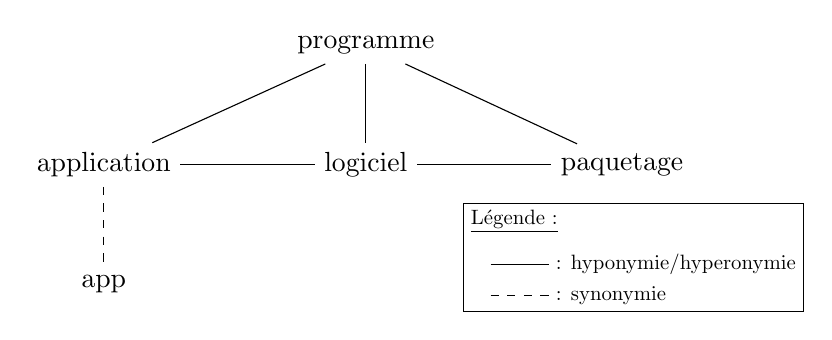
\begin{tikzpicture}
            \node (programme) {programme};
            \node [below=of programme] (logiciel) {logiciel};
            \node [right=of logiciel, xshift=2em] (paquetage) {paquetage};
            \node [left=of logiciel, xshift=-2em] (application) {application};
            \node [below=of application] (app) {app};

            \draw (programme) -- (logiciel);
            \draw (programme) -- (application);
            \draw (programme) -- (paquetage);
            \draw (application) -- (logiciel);
            \draw (logiciel) -- (paquetage);
            \draw [dashed] (application) -- (app);

            % legend
            \node [scale=.75, right=of app, xshift=12em, yshift=3em] (legend_title) {\underline{Légende~:}};
            \node [scale=.75, below=of legend_title, xshift=-1.5em, yshift=3em] (begin_hyponym) {};
            \node [scale=.75, right=of begin_hyponym, xshift=-1em] (end_hyponym) {: hyponymie/hyperonymie};
            \node [scale=.75, below=of begin_hyponym, yshift=3em] (begin_synonym) {};
            \node [scale=.75, right=of begin_synonym, xshift=-1em] (end_synonym) {: synonymie};

            \draw (legend_title.north  -| end_hyponym.east) rectangle (end_synonym.south -| legend_title.west);

            \draw (begin_hyponym) -- (end_hyponym);
            \draw [dashed] (begin_synonym) -- (end_synonym);
          \end{tikzpicture}
          \caption{Exemple de chaîne lexicale~\cite{ercan2007lexicalchains}
                   \label{fig:lexical_chain}}
        \end{figure}

        ~\\Tirant aussi profit d'arbres de décision, \newcite{lopez2010humb}
        sont les vainqueurs de la campagne d'évaluation
        SemEval-2010~\cite{kim2010semeval}. Ils extraient les termes-clés\index{terme-cle@Terme-clé} en
        deux étapes. Tout d'abord, ils ordonnent les termes-clés\index{terme-cle@Terme-clé} candidats avec
        les arbres de décision, puis ils les ré-ordonnent à la manière de
        \newcite{turney2003keacoherence}~: les candidats bien classés
        initialement sont d'autant mieux classés qu'ils ont un fort lien
        sémantique avec d'autres candidats bien classés initialement.

      \subsubsection{Séparateurs à vastes marges}
      \label{subsubsec:main-state_of_the_art-automatic_keyphrase_extraction-supervised_keyphrase_extraction-svms}
        Les séparateurs à vastes marges (\textsc{Svm}) projettent les exemples\index{exemple@Exemple}
        et les contre-exemples\index{exemple@Exemple} du corpus d'entraînement sur un plan (ou
        hyperplan) selon la
        valeur de leurs traits, puis cons\-truisent la droite (l'hyperplan) qui les sépare.
        Pour classer les termes-clés\index{terme-cle@Terme-clé} candidats d'un document\index{document@Document}, il suffit ensuite
        de les projeter sur ce même plan et d'utiliser l'hyperplan appris.

        ~\\\newcite{zhang2006svm} utilisent un \textsc{Svm} pour extraire les
        termes-clés\index{terme-cle@Terme-clé} à partir de ce qu'ils appellent le contexte global et le
        contexte local des termes-clés\index{terme-cle@Terme-clé} candidats. Ils représentent le contexte
        global d'un candidats par son \textsc{Tf-Idf\index{tf-idf@TF-IDF}}, sa première position et
        ses occurrences dans différentes parties du document\index{document@Document}, tandis qu'ils
        représentent son contexte local par sa catégorie grammaticale et trois
        traits encore jamais utilisés auparavant. Les deux premiers traits sont
        déterminés à partir des dépendances entre les mots\index{mot@Mot}.
        L'un dénote le nombre\index{nombre@Nombre} de fois que le candidat modifie un mot\index{mot@Mot}
        et l'autre dénote le nombre\index{nombre@Nombre} de fois qu'un mot\index{mot@Mot} modifie le candidat. Le
        dernier trait s'appelle le \textsc{Tf-Idf\index{tf-idf@TF-IDF}} contextuel, il s'agit de la
        somme du \textsc{Tf-Idf\index{tf-idf@TF-IDF}} de tous les mots\index{mot@Mot} qui cooccurrent avec le
        candidat. Ce dernier trait est intéressant, il indique si un candidat occurre dans un
        contexte important vis-à-vis du document\index{document@Document}.

        ~\\\newcite{jiang2009rankingsvm} extraient les termes-clés\index{terme-cle@Terme-clé} à partir d'un
        type particulier de \textsc{Svm}, baptisé
        \textsc{Svm}$^\textnormal{rank}$. \textsc{Svm}$^\textnormal{rank}$
        construit plusieurs hyperplans qui permettent d'ordonner les termes-clés\index{terme-cle@Terme-clé}
        candidats. Utilisant le score\index{score@Score} \textsc{Tf-Idf\index{tf-idf@TF-IDF}} des candidats, leur taille
        (en nombre\index{nombre@Nombre} de mots\index{mot@Mot}), leur première position, leur entropie et d'autres
        traits, le travail de \newcite{jiang2009rankingsvm} montre que le
        classifieur\index{classifieur@Classifieur} \textsc{Svm}$^\textnormal{rank}$ est plus performant qu'un
        \textsc{Svm} ou qu'un classifieur\index{classifieur@Classifieur} naïf bayesien utilisant les mêmes
        traits.

        ~\\\newcite{eichler2010keywe} extraient eux aussi les termes-clés\index{terme-cle@Terme-clé} à
        partir d'un \textsc{Svm}$^\textnormal{rank}$. Ils apprennent le
        \textsc{Svm}$^\textnormal{rank}$ avec trois valeurs pour le rang. La
        valeur maximale est attribuée aux exemples\index{exemple@Exemple} d'un document\index{document@Document}
        d'apprentissage, la valeur minimale aux contre-exemples\index{exemple@Exemple} du document\index{document@Document} et
        une valeur intermédiaire à ses contre-exemples\index{exemple@Exemple} qui sont des exemples\index{exemple@Exemple}
        d'autres documents\index{document@Document} d'apprentissage. Cette approche peut être assimilé à
        celle de \newcite{frank1999keafrequency}, qui estime qu'un terme-clé\index{terme-cle@Terme-clé}
        candidat fréquemment utilisé comme terme-clé\index{terme-cle@Terme-clé} dans le corpus
        d'apprentissage est plus vraisemblablement un terme-clé\index{terme-cle@Terme-clé}. Quant aux
        traits utilisés pour entraîner le \textsc{Svm}$^\text{rank}$, le plus
        notable se réfère à Wikipedia. L'intuition des auteurs est que si un
        terme-clé\index{terme-cle@Terme-clé} candidat fait l'objet d'un article Wikipedia, alors il est
        plus vraisemblablement un terme-clé\index{terme-cle@Terme-clé}.

      \subsubsection{Perceptrons multicouches}
      \label{subsubsec:main-state_of_the_art-automatic_keyphrase_extraction-supervised_keyphrase_extraction-neural_network}
        Les perceptrons multicouches sont des classifieurs qui émulent la
        biologie de l'apprentissage humain. Ce sont des réseaux de neurones
        répartis sur au moins trois couches. Les neurones de la première couche
        représentent les traits d'un candidat (un neurone par trait), ceux des
        couches intermédiaires (couches cachées) propagent des scores\index{score@Score} obtenus
        selon la valeur des traits et ceux de la dernière couche donnent un
        score\index{score@Score} final pour chaque classe \og{}terme-clé\index{terme-cle@Terme-clé}\fg{} et \og{}non
        terme-clé\index{terme-cle@Terme-clé}\fg{} (un neurone par classe). La classe ayant le plus haut
        score\index{score@Score} est celle du terme-clé\index{terme-cle@Terme-clé} candidat pour lequel correspond la valeur
        des traits. Optionnellement, les scores\index{score@Score} calculés pour chaque classe
        peuvent être utilisés pour déterminer le degré de confiance du
        perceptron pour la classe qu'il a
        attribué~\cite{denker1991neuralnetprobability}.
        
        ~\\\newcite{sarkar2010neuralnetwork} utilisent un perceptron
        multicouche. Les traits qu'ils emploient concer\-nent la fréquence du
        candidat, sa position et sa taille (en nombre\index{nombre@Nombre} de mots\index{mot@Mot}) ainsi que celle
        de ses mots\index{mot@Mot} (en nombre\index{nombre@Nombre} de caractères). Cette dernière est rarement
        utilisée comme trait pour l'extraction supervisée de termes-clés\index{terme-cle@Terme-clé}.
        L'hypothèse de \newcite{sarkar2010neuralnetwork} se fonde sur la loi de
        \newcite{zipf1935zipflaw}~: les mots\index{mot@Mot} courts étant plus fréquents que les
        mots\index{mot@Mot} longs, alors la taille d'un mot\index{mot@Mot} est une indication de sa rareté,
        donc de sa spécificité vis-à-vis du document\index{document@Document}.
        
        À la manière des méthodes\index{methode@Méthode} utilisant un classifieur\index{classifieur@Classifieur} probabiliste,
        \newcite{sarkar2010neuralnetwork} ordonnent les termes-clés\index{terme-cle@Terme-clé} candidats
        afin d'extraire un nombre\index{nombre@Nombre} donné de termes-clés\index{terme-cle@Terme-clé} lorsque nécessaire. Pour
        cela, ils utilisent le degré de confiance attribué à la
        classification~\cite{denker1991neuralnetprobability}. En premier sont
        placés les candidats classés \og{}terme-clé\index{terme-cle@Terme-clé}\fg{}, dans l'ordre
        décroissant du score\index{score@Score} de confiance~; en dernier sont placés les candidats
        classés \og{}non terme-clé\index{terme-cle@Terme-clé}\fg{}, dans l'ordre croissant du score\index{score@Score}
        de confiance. Ainsi, s'il y a plus de \og{}terme-clé\index{terme-cle@Terme-clé}\fg{} que requis,
        alors ceux ayant la plus haute confiance sont extrait. Inversement, s'il
        n'y a pas suffisamment de \og{}terme-clé\index{terme-cle@Terme-clé}\fg{}, alors des candidats
        classés \og{}non terme-clé\index{terme-cle@Terme-clé}\fg{} avec une confiance faible sont ajoutés.

      \subsubsection{Algorithmes génétiques}
      \label{subsubsec:main-state_of_the_art-automatic_keyphrase_extraction-supervised_keyphrase_extraction-genex}
        Les algorithmes génétiques sont des algorithmes qui donnent une solution
        approchée à un problème d'optimisation. Ce type d'algorithme
        n'effectue pas de classification et n'est pas nécessairement supervisé.

        ~\\\newcite{turney1999learningalgorithms} propose une méthode\index{methode@Méthode}
        supervisée, GenEx, dont les paramètres sont valués par un algorithme
        génétique, appelé \textit{Genitor}. Un algorithme d'extraction de
        termes-clés\index{terme-cle@Terme-clé}, appelé \textit{Extractor}, est appliqué sur le corpus
        d'apprentissage avec des paramètres initiaux, puis le \textit{Genitor}
        fait évoluer la valeur de ses paramètres jusqu'à trouver celle qui
        maximise les performances\index{performance@Performance} de l'extraction. L'extraction des termes-clés\index{terme-cle@Terme-clé}
        d'un document\index{document@Document} se fait ensuite avec l'\textit{Extractor} et ses
        paramètres configurés par le \textit{Genitor}. Les paramètres appris
        sont principalement des seuils limitant la taille des candidats, le
        nombre\index{nombre@Nombre} de mots\index{mot@Mot} importants à considérer pour filtrer les candidats, ou
        encore le nombre\index{nombre@Nombre} de termes-clés\index{terme-cle@Terme-clé} à extraire. Ce sont aussi des facteurs
        multiplicateurs utilisés notamment pour le calcul de l'importance\index{importance@Importance} des
        mots\index{mot@Mot} et des candidats.

      \subsubsection{Bilan des méthodes\index{methode@Méthode} supervisées}
      \label{subsubsec:main-state_of_the_art-automatic_keyphrase_extraction-supervised_keyphrase_extraction-conclusion}
        Les méthodes\index{methode@Méthode} supervisées reformulent la tâche d'extraction de
        termes-clés\index{terme-cle@Terme-clé} en une tâche de classification des termes-clés\index{terme-cle@Terme-clé} candidats en
        tant que \og{}terme-clé\index{terme-cle@Terme-clé}\fg{} ou \og{}non terme-clé\index{terme-cle@Terme-clé}\fg{}. Pour cela,
        elles utilisent des classifieurs et proposent divers traits pour
        discriminer les candidats. C'est par les traits qu'elles proposent que
        les méthodes\index{methode@Méthode} supervisées rivalisent. Certains traits sont génériques et
        communs à la majorité des méthodes\index{methode@Méthode}. C'est le cas de la position de la
        première occurrence du candidat et de son score\index{score@Score} \textsc{Tf-Idf\index{tf-idf@TF-IDF}}.
        D'autres traits sont spécifiques à certains types de documents\index{document@Document}. Par
        exemple\index{exemple@Exemple}, la section dans laquelle occurre un terme-clé\index{terme-cle@Terme-clé} est un trait
        discriminant pour l'extraction de termes-clés\index{terme-cle@Terme-clé} à partir d'articles
        journalistiques.

        Pour fonctionner, les méthodes\index{methode@Méthode} supervisées requièrent une collection de
        documents\index{document@Document} dits \og{}d'apprentissage\fg{}, ou \og{}d'entraînement\fg{}.
        Les documents\index{document@Document} de cette collection doivent être en nombre\index{nombre@Nombre} suffisant et
        être proches (par exemple\index{exemple@Exemple}, en terme de genre) des documents\index{document@Document} qui doivent
        être traités par la suite.

  \section{Assignement automatique\index{assignement automatique@Assignement automatique} de termes-clés\index{terme-cle@Terme-clé}}
  \label{sec:main-state_of_the_art-automatic_keyphrase_assignment}
    L'assignement automatique\index{assignement automatique@Assignement automatique} de termes-clés\index{terme-cle@Terme-clé} fait l'objet de moins de travaux
    que l'extraction. Il s'agit aussi d'une tâche plus difficile, car elle doit
    assigner des entrées d'un vocabulaire\index{vocabulaire@Vocabulaire} contrôlé en tant que termes-clés\index{terme-cle@Terme-clé} d'un
    document\index{document@Document} indépendamment de leur présence dans celui-ci.

    ~\\\newcite{medelyan2006kea++} sont les premiers à proposer une
    méthode\index{methode@Méthode} capable de faire de l'assignement de termes-clés\index{terme-cle@Terme-clé}. Celle-ci,
    \textsc{Kea}++, améliore la méthode\index{methode@Méthode} d'extraction \textsc{Kea}. Pour cela,
    elle utilise un thésaurus\footnote{Thésaurus~: liste de termes regroupés
    selon les concepts d'un domaine\index{domaine@Domaine} de connaissance qu'ils représentent.} du
    domaine\index{domaine@Domaine} de spécialité\index{specialite@Spécialité} à traiter. Il est mis à profit de deux manières~:
    d'abord pour sélectionner les termes-clés\index{terme-cle@Terme-clé} candidats, ensuite pour améliorer
    la classification.

    \newcite{medelyan2006kea++} décident de réaliser l'assignement en se
    limitant aux termes-clés\index{terme-cle@Terme-clé} qui occurrent dans le document\index{document@Document}. Ils sélectionnent
    donc toutes les unités textuelles\index{unite textuelle@Unité textuelle} qui correspondent à une entrée du
    thésaurus. À l'instar des candidats de \textsc{Kea}, ceux de \textsc{Kea++}
    sont ensuite classés en tant que \og{}terme-clé\index{terme-cle@Terme-clé}\fg{} ou \og{}non
    terme-clé\index{terme-cle@Terme-clé}\fg{} par un classifieur\index{classifieur@Classifieur} naïf bayesien. Ce classifieur\index{classifieur@Classifieur} est le même
    que celui de \textsc{Kea}, à l'exception d'un trait supplémentaire~: le
    nombre\index{nombre@Nombre} de relations sémantiques qu'entretient le candidat avec les autres
    dans le thésaurus. De cette manière, ils déterminent l'importance\index{importance@Importance} du
    candidats dans le domaine\index{domaine@Domaine}.

    Évaluée avec des documents\index{document@Document} du domaine\index{domaine@Domaine} agroalimentaire et le thésaurus
    Agrovoc\footnote{\url{http://aims.fao.org/standards/agrovoc}},
    la méthode\index{methode@Méthode} \textsc{Kea}++ double les performances\index{performance@Performance} de \textsc{Kea}. Le travail de
    \newcite{medelyan2006kea++} montre donc l'efficacité d'une méthode\index{methode@Méthode}
    d'assignement de termes-clés\index{terme-cle@Terme-clé}, même limitée.

    ~\\Au cours de la campagne d'évaluation
    Bio\textsc{Asq}~\cite{partalas2013bioasq}, nous assistons à une
    reformulation du problème d'assignement de termes-clés\index{terme-cle@Terme-clé} en un problème de
    classification multi-étiquette multi-classe. Les systèmes proposés lors de
    cette campagne attribuent des étiquettes au document\index{document@Document} en choisissant leur
    valeur parmi les entrées du vocabulaire\index{vocabulaire@Vocabulaire} contrôlé, soit les classes que peut
    prendre le document\index{document@Document}.

    Le problème de classification multi-étiquette multi-classe est généralement
    considéré comme de multiples problèmes de classification binaire. Soit un
    classifieur\index{classifieur@Classifieur} est appris pour chaque classe~; Soit un classifieur\index{classifieur@Classifieur} est appris
    pour chaque paire de classes et les classes retenues sont celles proposées
    par le plus de classifieurs. Ce type de classification, comparée à celle de
    \textsc{Kea}++, est donc plus coûteux, mais il présente l'avantage de
    permettre un assignement sans se limiter aux entrées du vocabulaire\index{vocabulaire@Vocabulaire} contrôlé
    présentes dans le document\index{document@Document}.

    ~\\\newcite{liu2011vocabularygap} proposent une méthode\index{methode@Méthode} que nous assimilons
    à de l'assignement de termes-clés\index{terme-cle@Terme-clé}. Ils font l'hypothèse qu'un document\index{document@Document} et
    ses termes-clés\index{terme-cle@Terme-clé} expriment le même contenu, mais dans deux langues
    différentes~: l'une expressive et l'autre synthétique. Ils reformulent donc
    la tâche d'indexation par termes-clés\index{terme-cle@Terme-clé} en une tâche de traduction du langage
    naturel vers celui des termes-clés\index{terme-cle@Terme-clé}.
    
    \newcite{liu2011vocabularygap} apprennent un modèle de traduction
    \textit{\textsc{Ibm} Model-1}~\cite{brown1993ibmmodel1} à l'aide de paires
    de mots\index{mot@Mot}~: un mot\index{mot@Mot} du langage naturel, l'autre du langage synthétique des
    termes-clés\index{terme-cle@Terme-clé}. Les mots\index{mot@Mot} du langage naturel sont extraits du document\index{document@Document} et les
    mots\index{mot@Mot} du langage synthétique sont extrait soit de son titre, soit de son
    résumé. Le modèle de traduction peut ensuite être appliqué aux termes-clés\index{terme-cle@Terme-clé}
    candidats, pour réaliser de l'extraction de termes-clés\index{terme-cle@Terme-clé} à la manière des
    classifieurs probabilistes présentés dans la
    section~\ref{subsubsec:main-state_of_the_art-automatic_keyphrase_extraction-supervised_keyphrase_extraction-probabilistic_models}
    (page~\pageref{subsubsec:main-state_of_the_art-automatic_keyphrase_extraction-supervised_keyphrase_extraction-probabilistic_models}),
    ou être utilisé pour générer une traduction, c'est-à-dire des termes-clés\index{terme-cle@Terme-clé}.

    Parce qu'elle est capable de générer des termes-clés\index{terme-cle@Terme-clé}, cette méthode\index{methode@Méthode} est
    intéressante. Cependant, il ne s'agit là que d'un premier pas vers
    l'assignement de termes-clés\index{terme-cle@Terme-clé}, car aucun vocabulaire\index{vocabulaire@Vocabulaire} n'est utilisé pour
    contrôler la génération.

    ~\\Alors que l'assignement attribue des termes-clés\index{terme-cle@Terme-clé} d'une qualité certifiée
    grâce au vocabulaire\index{vocabulaire@Vocabulaire} contrôlé, cette tâche n'est encore que très peu
    étudiée. Seulement deux travaux originaux s'en rapprochent. L'un se fonde
    sur un vocabulaire\index{vocabulaire@Vocabulaire} contrôlé (un thésaurus), mais ne va pas au-delà du
    contenu du document\index{document@Document}~; l'autre génère des termes-clés\index{terme-cle@Terme-clé} qui n'occurrent pas
    nécessairement dans le document\index{document@Document}, mais ne se fonde pas sur un vocabulaire\index{vocabulaire@Vocabulaire}
    contrôlé.

  %-----------------------------------------------------------------------------

  \section{Évaluation automatique de l'indexation par termes-clés\index{terme-cle@Terme-clé}}
  \label{sec:main-state_of_the_art-automatic_evaluation_of_keyphrase_annotation}
    Pour montrer l'apport des nouvelles méthodes\index{methode@Méthode} d'indexation par termes-clés\index{terme-cle@Terme-clé},
    celles-ci sont comparées automatiquement aux méthodes\index{methode@Méthode} existantes dans un
    processus d'évaluation \og{}à la Cranfield\fg{}
    \citep{voorhees2002philosophy}. Chaque méthode\index{methode@Méthode} est appliquée à un ensemble\index{ensemble@Ensemble}
    de documents\index{document@Document} de test (collection de test), les termes-clés\index{terme-cle@Terme-clé} qu'elle fournit
    pour chaque document\index{document@Document} sont mis en correspondance \og{}exacte\fg{} avec les
    termes-clés\index{terme-cle@Terme-clé} attribués manuellement aux documents\index{document@Document} (jugements de
    référence\index{reference@Référence})\footnote{Les termes-clés\index{terme-cle@Terme-clé} de référence\index{reference@Référence} sont soit les termes-clés\index{terme-cle@Terme-clé}
    des auteurs, soit les termes-clés\index{terme-cle@Terme-clé} de lecteurs (personnes lambda ou
    professionnelles), soit la combinaison des deux.}, puis évalués selon
    différents critères. Pour chaque critère, c'est la méthode\index{methode@Méthode} qui obtient les
    meilleurs\index{meilleur@Meilleur} résultats\index{resultat@Résultat} en moyenne qui est jugée la plus efficace.
  
    La mise en correspondance des termes-clés\index{terme-cle@Terme-clé} extraits/assignés aux termes-clés\index{terme-cle@Terme-clé}
    de référence\index{reference@Référence} sert à distinguer ceux qui sont corrects de ceux qui ne le sont
    pas. Nous parlons, respectivement, de vrais positifs et de faux positifs
    (voir le
    tableau\index{tableau@Tableau}~\ref{tab:confusion_matrix}). De la même manière, toute autre unité
    textuelle non extraite/assignée par la méthode\index{methode@Méthode} automatique est appelée faux
    négatif si elle correspond à un terme-clé\index{terme-cle@Terme-clé} de référence\index{reference@Référence}, et vrai négatif dans
    le cas contraire.
    
    D'après le paradigme d'évaluation \og{}à la Cranfield\fg{}, un
    vrai positif ne peut être considéré comme tel que s'il est strictement
    identique à un terme-clé\index{terme-cle@Terme-clé} de référence\index{reference@Référence}. Cette correspondance \og{}exacte\fg{}
    induit une évaluation pessimiste des méthodes\index{methode@Méthode} d'indexation automatique\index{indexation automatique@Indexation automatique} par
    termes-clés\index{terme-cle@Terme-clé}, car les variantes des termes-clés\index{terme-cle@Terme-clé} de référence\index{reference@Référence} sont jugées
    incorrectes sans distinction avec les autres faux positifs. Pour minimiser
    ce problème, toutes les évaluations réalisées dans la littérature tiennent
    compte uniquement du radical des mots\index{mot@Mot} des termes-clés\index{terme-cle@Terme-clé}, c'est-à-dire leur
    forme privée de tout suffixe (par exemple\index{exemple@Exemple}, \og{}empir\fg{} est le radical de
    \og{}empirique\fg{}). Les différences d'accords en genre et en
    nombre\index{nombre@Nombre} sont donc autorisées, ainsi que toute autre dérivation suffixale.
    Cette approche n'est pas parfaite, car elle fait parfois correspondre des
    mots\index{mot@Mot} porteurs de sens différents (par exemple\index{exemple@Exemple}, \og{}empire\fg{} et
    \og{}empirique\fg{} possèdent la même racine \og{}empir\fg{}). Une approche
    plus rigoureuse serait d'utiliser les lemmes des mots\index{mot@Mot}, c'est-à-dire leur
    forme conventionnelle (celle que nous retrouvons dans  un dictionnaire).
    Contrairement à la racinisation, qui applique seulement des règles de
    désuffixage (par exemple\index{exemple@Exemple}, \textit{-es $\rightarrow$ -} afin d'enlever l'accord du
    féminin pluriel), la lemmatisation requiert un lexique et doit être
    appliquée selon le context du mot\index{mot@Mot} à analyser (par exemple\index{exemple@Exemple}, le lemme de
    \og{}couvant\fg{} est soit \og{}couvant\fg{}, soit \og{}couver\fg{} selon
    son contexte). Pour des raisons pratiques, la lemmatisation n'est donc jamais
    utilisée pour l'évaluation automatique de termes-clés\index{terme-cle@Terme-clé}.
    \begin{table}
      \begin{center}
        \begin{tabular}{cc|cc}
          \toprule
          \multicolumn{2}{c|}{} & \multicolumn{2}{c}{\textbf{Jugement de référence}}\\
          \multicolumn{2}{c|}{} & \og{}terme-clé\fg{} & \og{}non terme-clé\fg{}\\
          \hline
          \multirow{2}{*}{\textbf{Résultat}} & \og{}terme-clé\fg{} & vrai positif ($\textsc{Vp}$) & faux positif ($\textsc{Fp}$)\\
          & \og{}non terme-clé\fg{} & faux negatif ($\textsc{Fn}$) & vrai negatif ($\textsc{Vn}$)\\
          \bottomrule
        \end{tabular}
        \caption{Matrice de confusion pour l'évaluation des méthodes
                 d'indexation automatique par termes-clés
                \label{tab:confusion_matrix}}
      \end{center}
    \end{table}

    Les critères d'évaluation utilisés pour évaluer et comparer les méthodes\index{methode@Méthode}
    d'indexation par termes-clés\index{terme-cle@Terme-clé} sont la précision, le rappel et la f1-mesure.
    La précision capture la capacité d'une méthode\index{methode@Méthode} à minimiser les erreurs (voir
    l'équation~\ref{math:precision}). Inversement, le rappel mesure la capacité de
    la méthode\index{methode@Méthode} à fournir le plus possible de termes-clés\index{terme-cle@Terme-clé} corrects (voir l'équation~\ref{math:recall}). Quant à la f1-mesure, elle évalue le compromis
    entre précision et rappel, c'est-à-dire la capacité de la méthode\index{methode@Méthode} à extraire
    un maximum de termes-clés\index{terme-cle@Terme-clé} corrects tout en faisant un minimum d'erreurs
    (voir l'équation~\ref{math:f1_measure}).
    \begin{align}
      \text{précision} &= \frac{\#\textsc{Vp}}{\#\textsc{Vp} + \#\textsc{Fp}} \label{math:precision}\\
      \text{rappel} &= \frac{\#\textsc{Vp}}{\#\textsc{Vp} + \#\textsc{Fn}} \label{math:recall}\\
      \text{f-mesure} &= (1 + \beta^2) \times \frac{\text{précision} \times \text{rappel}}{(\beta^2 \times \text{précision}) + \text{rappel}} \label{math:f_measure}\\
      \text{f1-mesure} &= 2 \times \frac{\text{précision} \times \text{rappel}}{\text{précision} + \text{rappel}} \label{math:f1_measure}
    \end{align}
      
%    En \textsc{Ri}, il est courant d'évaluer les méthodes\index{methode@Méthode} selon la qualité de
%    leur ordonnancement. Prenons l'exemple\index{exemple@Exemple} des moteurs de recherche, si deux
%    moteurs de recherche doivent fournir dix documents\index{document@Document} répondant à une requête
%    et que les deux systèmes n'ont que deux propositions pertinentes, alors ils
%    ont tous les deux la même précision (20~\%) et le même rappel (20~\%).
%    Toutefois, si le premier système classe ces documents\index{document@Document} en premier et que le
%    second système les classe aux positions neuf et dix, alors le premier
%    système est le meilleur\index{meilleur@Meilleur}. Lorsque les méthodes\index{methode@Méthode} d'indexation par termes-clés\index{terme-cle@Terme-clé}
%    le permettent, il est intéressant de mesurer leur capacité à classer en
%    premier les vrais positifs. Dans la littérature, quatre mesures, dont
%    certaines empruntées à la \textsc{Ri}, sont utilisées~: la \textsc{Map}
%    (\textit{Mean Average Precision}), la Bpref (\textit{Binary Preference
%    Measure}), la R-précision et la \textsc{Mrr} (\textit{Mean Reciprocal
%    Rank}). La \textsc{Map} mesure pour chaque document\index{document@Document} la moyenne de la
%    précision à chaque rang ($\textnormal{précision}@\textnormal{rang}$) d'un
%    vrai positif (voir l'équation~\ref{math:average_precision}). Avec la Bpref, la
%    \textsc{Map} est la seule mesure qui tient compte de tous les vrais
%    positifs. La Bpref est une mesure similaire à la \textsc{Map} qui,
%    contrairement à cette dernière, s'abstrait de la connaissance de tous les
%    termes-clés\index{terme-cle@Terme-clé} de référence\index{reference@Référence} (voir l'équation~\ref{math:bpref}). Elle peut donc,
%    par exemple\index{exemple@Exemple}, s'appliquer dans le cadre d'évaluations manuelles\index{evaluation manuelle@Évaluation manuelle} où chaque
%    terme-clé\index{terme-cle@Terme-clé} fourni par la méthode\index{methode@Méthode} est jugé correct ou non par un évaluateur
%    humain et où tous les termes-clés\index{terme-cle@Terme-clé} du document\index{document@Document} ne sont pas connus. La
%    R-précision est une variante de la précision. Elle mesure cette dernière
%    dans le cas optimal (tous les termes-clés\index{terme-cle@Terme-clé} sont fournis et il n'y a aucune
%    erreur), soit au rang $R$, où $R$ est égal au nombre\index{nombre@Nombre} de termes-clés\index{terme-cle@Terme-clé} de
%    référence\index{reference@Référence} du document\index{document@Document} (voir l'équation~\ref{math:r_precision}). Quant à la
%    \textsc{Mrr}, celle-ci est la moins précise, elle ne s'intéresse qu'au
%    meilleur\index{meilleur@Meilleur} rang obtenu pour un vrai positif (voir l'équation~\ref{math:reciprocal_rank}).
%    \begin{align}
%      \textsc{Map} &= \frac{\mathlarger{\sum}_{\text{\textit{terme-clé\index{terme-cle@Terme-clé}}} = \textsc{Vp}}\text{précision}@\text{rang}(\text{\textit{terme-clé\index{terme-cle@Terme-clé}}})}{\#\textsc{Vp} + \#\textsc{Fn}} \label{math:average_precision}\\
%      \notag \\
%      \text{Bpref} &= \sum_{\text{\textit{terme-clé\index{terme-cle@Terme-clé}}} = \textsc{Vp}}{1 - \frac{|\text{\textit{terme-clé\index{terme-cle@Terme-clé}}'}\ \text{de meilleur\index{meilleur@Meilleur} rang que}\ \text{\textit{terme-clé\index{terme-cle@Terme-clé}}}|}{\#\textsc{Vp} + \#\textsc{Fp}}} \label{math:bpref}\\
%      \notag \\
%      \text{R-précision} &= \text{précision}@(\#\textsc{Vp} + \#\textsc{Fn}) \label{math:r_precision}\\
%      \notag \\
%      \textsc{Mrr} &= \frac{1}{\text{argmin}(\forall \text{\textit{terme-clé\index{terme-cle@Terme-clé}}} = \textsc{Vp}, \text{rang}(\text{\textit{terme-clé\index{terme-cle@Terme-clé}}}))} \label{math:reciprocal_rank}
%    \end{align}

%    Toutes les mesures présentées précédemment respectent le paradigme de
%    l'évaluation \og{}à la Cranfield\fg{}. Cependant, associer des termes-clés\index{terme-cle@Terme-clé} à
%    un document\index{document@Document} est une tâche subjective~\cite{hasan2014state_of_the_art}, il
%    n'existe donc pas une solution unique. Des travaux proposent d'apporter plus
%    de souplesse à la comparaison entre termes-clés\index{terme-cle@Terme-clé} résultant d'une méthode\index{methode@Méthode} et
%    termes-clés\index{terme-cle@Terme-clé} de référence\index{reference@Référence} en tenant compte de leur
%    chevauchement~\cite{zesch2009rprecision,kim2010rprecision}. Ces travaux
%    ne sont toutefois pas utilisés travaux récents.

  %-----------------------------------------------------------------------------

  \section{Conclusion}
  \label{sec:main-state_of_the_art-automatic_evaluation_of_keyphrase_annotation-conclusion}
    Nous avons présenté la tâche d'indexation par termes-clés\index{terme-cle@Terme-clé}, de la sélection\index{selection@Sélection}
    des termes-clés\index{terme-cle@Terme-clé} candidats aux différentes méthodes\index{methode@Méthode} d'extraction et
    d'assignement de termes-clés\index{terme-cle@Terme-clé}, en passant par le processus d'évaluation
    automatique de ces dernières.

    La sélection\index{selection@Sélection} des termes-clés\index{terme-cle@Terme-clé} candidats est une étape quasi-systématique de
    l'extraction automatique\index{extraction automatique@Extraction automatique} de termes-clés\index{terme-cle@Terme-clé}. Ne s'agissant cependant pas du
    c\oe{}ur de la tâche, la définition de nouvelle méthodes\index{methode@Méthode} de sélection\index{selection@Sélection} est
    négligée au profit de méthodes\index{methode@Méthode} de sélection\index{selection@Sélection} simples (sélection\index{selection@Sélection} de n-grammes\index{n-gramme@N-gramme},
    \textit{chunks} nominaux ou séquences de noms\index{nom@Nom} et d'adjectifs\index{adjectif@Adjectif}). Toutefois,
    l'idée que l'indexation par termes-clés\index{terme-cle@Terme-clé} gagnerait en performances\index{performance@Performance} si les
    candidats sélectionnés étaient moins nombreux, c'est-à-dire contiendraient
    moins d'erreurs, semble faire consensus auprès des chercheurs qui s'y
    intéressent~\cite{huang2006semanticnetworkstructureanalysis,wang2014keyphraseextractionpreprocessing}. La méthode\index{methode@Méthode} qui
    consiste à définir des patrons grammaticaux, tels que celui pour
    sélectionner les plus longues séquences de noms\index{nom@Nom} et d'adjectifs\index{adjectif@Adjectif}, pourrait
    être utilisée pour sélectionner des candidats en s'intéressant plus en
    profondeur aux classes grammaticales employées dans les termes-clés\index{terme-cle@Terme-clé}, ainsi
    qu'à d'autres propriétés linguistiques de leurs composants.

    Le c\oe{}ur de la tâche d'indexation automatique\index{indexation automatique@Indexation automatique} par termes-clés\index{terme-cle@Terme-clé} est
    réalisé de deux manières différentes~: soit les termes-clés\index{terme-cle@Terme-clé} sont extraits
    depuis le contenu du document\index{document@Document}, soit ils sont assignés en puisant dans un
    vocabulaire\index{vocabulaire@Vocabulaire} contrôlé. Dans la littérature, l'extraction fait l'objet de plus
    de travaux que l'assignement. Elle est plus simple à mettre en \oe{}uvre,
    car elle analyse les unités textuelles\index{unite textuelle@Unité textuelle} présentent dans le document\index{document@Document}, tandis
    que l'assignement doit pouvoir déterminer si une entrée du vocabulaire\index{vocabulaire@Vocabulaire}
    contrôlé (n'occurrant pas nécessairement dans le document\index{document@Document}) est importante
    vis-à-vis de celui-ci. Par ailleurs, la seule méthode\index{methode@Méthode} réalisant actuellement
    l'assignement se limite aux entrées présentent dans le document\index{document@Document}, tant il
    peut parfois être difficile d'établir le lien entre celles qui n'y sont pas
    et le contenu du document\index{document@Document}.

    L'évaluation des méthodes\index{methode@Méthode} d'indexation par termes-clés\index{terme-cle@Terme-clé} est généralement
    effectuée de manière automatique. Comparé à un jugement de référence\index{reference@Référence} unique,
    le résultat\index{resultat@Résultat} d'une méthode\index{methode@Méthode} d'indexation par termes-clés\index{terme-cle@Terme-clé} est évalué en termes
    de précision, qui est d'autant plus élevée s'il y a le moins d'erreurs, de
    rappel, qui est d'autant plus élevée s'il y a beaucoup de termes-clés\index{terme-cle@Terme-clé}
    positifs, et de f1-mesure, qui est le compromis entre précision et rappel.
    Ce modèle d'évaluation présente l'avantage d'être utilisable dès lors que
    des données de test sont disponibles. La comparaison à un jugement de
    référence\index{reference@Référence} unique rend cependant l'évaluation pessimiste. Lorsque les
    conditions le permettent, une évaluation manuelle\index{evaluation manuelle@Évaluation manuelle} reste indispensable pour
    mieux mesurer les forces et les faiblesses d'une méthode\index{methode@Méthode} d'indexation par
    termes-clés\index{terme-cle@Terme-clé}.


  \chapter{Ressources}
\label{chap:main-data_description}
  \chaptercite{
    [...] pour comprendre précisément les forces et les faiblesses d'un
    système d'extraction de termes-clés\index{terme-cle@Terme-clé}, il est essentiel de l'évaluer avec
    différentes collections de données.
%    [...] to fully understand the strengths and weaknesses of a keyphrase
%    extractor, it is essential to evaluate it on multiple datasets.
  }{
    \newcite{hassan2010conundrums}
  }{.75\linewidth}{\justify}

  \section{Introduction}
  \label{sec:main-data_description-introduction}
    En indexation automatique\index{indexation automatique@Indexation automatique} par termes-clés\index{terme-cle@Terme-clé}, des
    collections de données sont nécessaires à l'évaluation et à la comparaison
    des nouveaux travaux aux précédents. Elles sont généralement réparties en
    deux ensembles\index{ensemble@Ensemble}~: un ensemble\index{ensemble@Ensemble} de documents\index{document@Document} d'entraînement (ou
    d'apprentissage), dont les termes-clés\index{terme-cle@Terme-clé} de référence\index{reference@Référence} servent à paramétrer ou
    à entraîner une méthode\index{methode@Méthode}, et un ensemble\index{ensemble@Ensemble} de documents\index{document@Document} de test, dont les
    termes-clés\index{terme-cle@Terme-clé} de référence\index{reference@Référence} servent à évaluer les performances\index{performance@Performance} d'une méthode\index{methode@Méthode}.
    De nombreuses collections sont accessibles publiquement\footnote{Un grand
    nombre\index{nombre@Nombre} de collections de données est accessible depuis le dépôt GitHub de Su
    Nam Kim (\textit{snkim})~:
    \url{https://github.com/snkim/AutomaticKeyphraseExtraction}.}, elles
    couvrent plusieurs langues (français, anglais, etc.), domaines\index{domaine@Domaine}
    (météorologie, sciences humaines et sociales, informatique, etc.) et genres
    de documents\index{document@Document} (résumés, articles scientifiques, articles journalistiques,
    etc.). Cette diversité est essentielle à la compréhension des points forts
    et des points faibles d'une méthode\index{methode@Méthode} d'indexation par termes-clés\index{terme-cle@Terme-clé}, car des
    facteurs différents peuvent influencer ses performances\index{performance@Performance}.
    \newcite{hasan2014state_of_the_art} en énoncent quatre~:
    \begin{itemize}
      \item{si un document\index{document@Document} est long, alors le nombre\index{nombre@Nombre} de termes-clés\index{terme-cle@Terme-clé} candidats
            pour celui-ci est élevé et l'indexation par termes-clés\index{terme-cle@Terme-clé} est plus
            difficile que pour un document\index{document@Document} court~;}
      \item{si le contenu d'un document\index{document@Document} est structuré (par exemple\index{exemple@Exemple} un article
            scientifique réparti en sections), alors une méthode\index{methode@Méthode} tenant compte
            de cette structure est avantagée~;}
      \item{si des changements thématiques surviennent dans un document\index{document@Document}, une
            méthode\index{methode@Méthode} qui utilise la position de la première occurrence des
            candidats peut être désavantagée~;}
      \item{si des sujets\index{sujet@Sujet} sans relation sont abordés dans un même document\index{document@Document},
            alors une méthode\index{methode@Méthode} qui tisse des liens sémantiques entre les
            termes-clés\index{terme-cle@Terme-clé} candidats est pénalisée.}
    \end{itemize}
    Des variations de performance\index{performance@Performance} dues à la mauvaise qualité de certains
    documents\index{document@Document} sont aussi constatées. Dans le cas d'articles scientifiques, par
    exemple\index{exemple@Exemple}, les documents\index{document@Document} sont fréquemment issus d'un \textsc{Pdf}
    (\textit{Portable Document\index{document@Document} Format}), puis convertis en texte depuis ses flux
    de données ou avec des outils d'\textsc{Ocr} (\textit{Optical Character
    Recognition}). Ces procédés ne sont pas parfaits, ils ajoutent parfois des
    fautes d'orthographe (mauvais caractères et problèmes d'accents) et ils ne
    traitent pas toujours correctement certains environnements graphiques et
    textuels tels que les notes de pieds de page, les tableaux\index{tableau@Tableau}, les figures et
    les équations. Nous identifions deux autres facteurs que
    \newcite{hasan2014state_of_the_art} n'évoquent pas. Selon les collections de
    données, la proportion de termes-clés\index{terme-cle@Terme-clé} de référence\index{reference@Référence} n'apparaissant pas dans
    les documents\index{document@Document} varie d'un extrême à l'autre. Dans le cas où la majorité des
    termes-clés\index{terme-cle@Terme-clé} n'apparaissent pas dans les documents\index{document@Document}, les méthodes\index{methode@Méthode} d'extraction
    de termes-clés\index{terme-cle@Terme-clé} sont désavantagées. La qualification des annotateurs des
    termes-clés\index{terme-cle@Terme-clé} de référence\index{reference@Référence} est le second facteur. Nous observons trois
    annotateurs différents~: les auteurs des articles, des indexeurs
    professionnels et des lecteurs. Les auteurs cherchent à attirer le lecteur~;
    les indexeurs professionnels (ou ingénieurs documentalistes) aspirent à une
    indexation homogène, et conforme au langage du domaine\index{domaine@Domaine}, de tous les
    documents\index{document@Document} d'un même domaine\index{domaine@Domaine} grâce à un vocabulaire\index{vocabulaire@Vocabulaire} contrôlé~; les lecteurs
    sont plus libres que les auteurs et les indexeurs professionnels, ils ne
    sont influencés ni par les termes-clés\index{terme-cle@Terme-clé} \og{}à la mode\fg{}, ni par un
    vocabulaire\index{vocabulaire@Vocabulaire} contrôlé.

    Dans nos travaux de recherche, nous utilisons cinq collections de données~:
    Termith, \textsc{De}ft, Wikinews, SemEval et \textsc{Duc}. En accord avec le
    point de vue de \newcite{hassan2010conundrums}, celles-ci couvrent deux
    langues (français et anglais), un large éventail de domaines\index{domaine@Domaine} (sciences
    humaines et sociales, informatique, météorologie, catastrophes naturelles,
    etc.) et trois gen\-res de documents\index{document@Document} (résumés, articles scientifiques et
    articles journalistiques). De plus, les annotateurs de chaque collection ont
    des qualifications différentes.

  %-----------------------------------------------------------------------------

  \section{Termith}
  \label{sec:main-data_description-termith_data}
    Le projet Termith et l'Inist mettent à notre disposition quatre collections
    de notices bibliographiques en domaines\index{domaine@Domaine} de spécialité\index{specialite@Spécialité}. Une notice
    bibliographique est une entrée d'un catalogue bibliographique. Elle décrit
    un document\index{document@Document} avec différentes métadonnées~: des informations factuelles
    (titre, auteurs, affiliation des auteurs, éditeur, résumé, termes-clés\index{terme-cle@Terme-clé} des
    auteurs, etc.) et des informations produites par un indexeur professionnel
    (résumé --- si nécessaire, termes-clés\index{terme-cle@Terme-clé}, etc.). Pour produire les
    termes-clés\index{terme-cle@Terme-clé}, l'indexeur professionnel a recours à des ressources et des
    pratiques documentaire~\cite{guinchat1996techniquesdocumentaires} qui
    assurent une indexation par termes-clés\index{terme-cle@Terme-clé} de qualité~: homogène, conforme au
    langage du domaine\index{domaine@Domaine} du document\index{document@Document}, spécifique au document\index{document@Document}, général du point de
    vue de son domaine\index{domaine@Domaine}, exhaustive et impartiale.
    
    \begin{table}
      \centering
      \resizebox{\linewidth}{!}{
        \begin{tabular}{l|c|c}
          \toprule
          Revue & Quantité de documents & Période de publication\\
          \hline
          A. sp. Anglais de spécialité & ~~99 & 2001 -- 2012\\
          Bulletin d'études orientales & ~~~~8 & 2008 -- 2010\\
          Cahiers de grammaire & ~~~~4 & ~~~~~~~~~~~~2000\\
          Cahiers de praxématique~: (Montpellier) & ~~44 & 2006 -- 2009\\
          Langue française~: (Paris. 1969) & ~~39 & 2011 -- 2012\\
          Les Cahiers de l'ILCEA & ~~20 & 2004 -- 2007\\
          Lidil~: (Grenoble) & ~~76 & 2005 -- 2011\\
          Linx & 146 & 2001 -- 2008\\
          Mots~: (Paris. 1980) & 112 & 2002 -- 2012\\
          Recherches linguistiques de Vincennes & ~~37 & 2001 -- 2010\\
          Travaux de linguistique~: (Gent) & 130 & 2001 -- 2005\\
          \bottomrule
        \end{tabular}
      }

      \caption{Détail des revues du corpus de linguistique (Termith)
               \label{tab:linguistics_journals}}
    \end{table}
    \begin{table}
      \centering
      \resizebox{\linewidth}{!}{
        \begin{tabular}{l|c|c}
          \toprule
          Revue & Quantité de documents & Période de publication\\
          \hline
          Communication~: (Montréal) & ~~~~2 & ~~~~~~~~~~~~2005\\
          Document numérique & 176 & 2001 -- 2012\\
          Documentaliste~: (Paris) & 385 & 2007 -- 2012\\
          Questions de communication~: (Nancy) & 135 & 2007 -- 2012\\
          Études de communication & ~~~~8 & ~~~~~~~~~~~~2009\\
          \bottomrule
        \end{tabular}
      }

      \caption{Détail des revues du corpus de sciences de l'information
               (Termith)
               \label{tab:information_sciences_journals}}
    \end{table}
    \begin{table}
      \centering
      \resizebox{\linewidth}{!}{
        \begin{tabular}{l|c|c}
          \toprule
          Revue & Quantité de documents & Période de publication\\
          \hline
          Annales de Bretagne et des pays de l'Ouest & ~~~~3 & 2001 -- 2008\\
          Archéosciences & ~~24 & 2007 -- 2011\\
          Arts asiatiques~: (Paris) & ~~36 & 2001 -- 2006\\
          Bulletin de correspondance hellénique & ~~~~9 & 2001 -- 2003\\
          Bulletin de l'Ecole française d'Extrême-Orient & ~~~~4 & ~~~~~~~~~~~~2001\\
          Bulletin de la Société préhistorique française & 163 & 2007 -- 2012\\
          Documents d'archéologie méridionale & ~~51 & 2001 -- 2006\\
          Gallia & ~~22 & 2001 -- 2007\\
          Gallia. Préhistoire & ~~26 & 2001 -- 2007\\
          Journal de la Société des océanistes & ~~~~2 & ~~~~~~~~~~~~2001\\
          Paléo~: (Les Eyzies de Tayac-Sireuil) & 137 & 2001 -- 2009\\
          Paléorient & ~~43 & 2001 -- 2007\\
          Préhistoire anthropologie méditerranéennes & ~~30 & 2003 -- 2005\\
          Revue archéologique de Picardie & ~~10 & 2001 -- 2007\\
          Revue archéologique de l'Est & ~~35 & 2005 -- 2011\\
          Revue archéologique de l'Ouest & ~~39 & 2006 -- 2011\\
          Revue archéologique du centre de la France & ~~13 & 2001 -- 2004\\
          Revue des études grecques~: (Paris) & ~~11 & 2002 -- 2012\\
          Revue numismatique~: (Paris) & ~~17 & 2001 -- 2005\\
          Syria & ~~~~7 & ~~~~~~~~~~~~2001\\
          Syria~: (Paris) & ~~18 & 2004 -- 2005\\
          Techniques \& culture~: (Paris) & ~~16 & 2003 -- 2010\\
          \bottomrule
        \end{tabular}
      }

      \caption{Détail des revues du corpus d'archéologie (Termith)
               \label{tab:archeology_journals}}
    \end{table}
    \begin{table}
      \centering
      \resizebox{\linewidth}{!}{
        \begin{tabular}{p{.533\linewidth}|c|c}
          \toprule
          Revue & Quantité de documents & Période de publication\\
          \hline
          Canadian Journal of Chemistry & 125 & 1983 -- 1991\\
          Comptes rendus de l'Académie des sciences. Série 2, Mécanique,
          physique, chimie, sciences de l'univers, sciences de la terre & 265 & 1985 -- 1990\\
          Comptes rendus de l'Académie des sciences. Série II, Mécanique,
          physique, chimie, astronomie & ~~70 & 1994 -- 1997\\
          Comptes rendus de l'académie des sciences. Série IIc, chimie & 124 & 1998 -- 2001\\
          Comptes rendus. Chimie & 200 & 2002 -- 2012\\
          \bottomrule
        \end{tabular}
      }

      \caption{Détail des revues du corpus de chimie (Termith)
               \label{tab:chemestry_journals}}
    \end{table}
    Les tableaux\index{tableau@Tableau}~\ref{tab:linguistics_journals}~à~\ref{tab:chemestry_journals}
    représentent la répartition, revue par revue, de chacune des collections. Le
    projet Termith s'intéresse principalement aux sciences humaines et sociales
    (\textsc{Shs}). De ce fait, trois de ses collections de notices représentent
    un domaine\index{domaine@Domaine} de \textsc{Shs}~: linguistique, sciences de l'information
    (sciences de l'info.) et archéologie. La quatrième collection représente la
    chimie. Le corpus de linguistique est constitué de 715 notices d'articles
    français paru entre 2000 et 2012 dans 11 revues~; le corpus des sciences de
    l'information contient 706 notices d'articles français publiés entre 2001 et
    2012 dans cinq revues~; le corpus d'archéologie est composé de 716 notices
    représentant des articles français paru entre 2001 et 2012 dans 22 revues~;
    le corpus de chimie est composé de 784 notices d'articles français publiés
    entre 1983 et 2012 dans cinq revues.

    Le tableau\index{tableau@Tableau}~\ref{tab:termith} présente les caractéristiques du corpus
    Termith. Chaque domaine\index{domaine@Domaine} est divisé en deux sous-ensembles\index{ensemble@Ensemble}\footnote{Les
    revues sont réparties équitablement entre chaque ensemble\index{ensemble@Ensemble}.}~: un ensemble\index{ensemble@Ensemble}
    d'apprentissage (appr.) composé de 506 à 582 notices selon le domaine\index{domaine@Domaine} et un
    ensemble\index{ensemble@Ensemble} de test contenant 200 notices. S'agissant de résumés, les documents\index{document@Document}
    sont courts (voir la figure~\ref{fig:example_inist}), ils ont en moyenne 123,9
    mots\index{mot@Mot}. Quant aux termes-clés\index{terme-cle@Terme-clé}, nous utilisons ceux produits par les indexeurs
    professionnels. Ils sont concis (un à deux mots\index{mot@Mot} principalement) et, du fait
    de la méthodologie d'indexation, ils ne sont majoritairement pas présents
    dans les résumés (ils sont \og{}à assigner\fg{}).
    \begin{table}[!h]
      \centering
      \resizebox{\linewidth}{!}{
        \begin{tabular}{l|c@{~~}c@{~~}c@{~~}c|c@{~~}c@{~~}c@{~~}c}
          \toprule
          \multirow{2}{*}{\textbf{Corpus}} & \multicolumn{4}{c|}{\textbf{Documents}} & \multicolumn{4}{c}{\textbf{Termes-clés}}\\
          \cline{2-9}
          & Langue & Genre & Quantité & Mots moy. & Annotateur & Quantité moy. & \og{}À assigner\fg{} & Mots moy.\\
          \hline
          Linguistique & & & & & & &\\
          \hfill{}Appr. & Français & Scientifique (résumé) & 515 & 160,5 & Professionnel & $~~$8,6 & 60,6~\% & 1,7\\
           \hfill{}Test & \ditto & \ditto & 200 & 147,0 & \ditto & $~~$8,9 & 62,8~\% & 1,8\\
          \hline
          Sciences de l'info. & & & & & & &\\
          \hfill{}Appr. & Français & Scientifique (résumé) & 506 & 105,0 & Professionnel & $~~$7,8 & 67,9~\% & 1,8\\
          \hfill{}Test & \ditto & \ditto & 200 & 157,0 & \ditto & 10,2 & 66,9~\% & 1,7\\
          \hline
          Archéologie & & & & & & &\\
          \hfill{}Appr. & Français & Scientifique (résumé) & 518 & 221,1 & Professionnel & 16,9 & 37,0~\% & 1,3\\
          \hfill{}Test & \ditto & \ditto & 200 & 213,9 & \ditto & 15,6 & 37,4~\% & 1,3\\
          \hline
          Chimie & & & & & & &\\
          \hfill{}Appr. & Français & Scientifique (résumé) & 582 & 105,7 &  Professionnel & 12,2 & 75,2~\% & 2,2\\
          \hfill{}Test & \ditto & \ditto & 200 & 103,9 & \ditto & 14,6 & 78,8~\% & 2,4\\
          \bottomrule
        \end{tabular}
      }

      \caption{Corpus Termith
               \label{tab:termith}}
    \end{table}

    \begin{figure}
      \framebox[\linewidth]{ % linguistique_11-0080464
        \parbox{.99\linewidth}{\footnotesize
          \textbf{La cause linguistique}
          \hfill\underline{\textit{Linguistique}}\\

          L'objectif est de fournir une définition de base du concept
          linguistique de la cause en observant son expression. Dans un premier
          temps, l'A. se demande si un tel concept existe en langue. Puis il
          part des formes de son expression principale et directe (les verbes et
          les conjonctions de cause) pour caractériser linguistiquement ce qui
          fonde une telle notion.\\

          \textbf{Termes-clés~:} français~; interprétation sémantique~;
          \underline{conjonction}~; expression linguistique~; \underline{concept
          linguistique}~; relation syntaxique~; \underline{cause}. 
        }
      }
      ~\\~\\
      \framebox[\linewidth]{ % sciencesInfo_08-0149317
        \parbox{.99\linewidth}{\footnotesize
          \textbf{Congrès de l'ABF~: les publics des bibliothèques}
          \hfill\underline{\textit{Sciences de l'info.}}\\

          Le cinquante-troisième congrès annuel de l'Association des
          bibliothécaires de France (ABF) s'est déroulé à Nantes du 8 au 10 juin
          2007. Centré sur le thème des publics, il a notamment permis de
          méditer les résultats de diverses enquêtes auprès des usagers,
          d'examiner de nouvelles formes de partenariats et d'innovations
          technologiques permettant aux bibliothèques de conquérir de nouveaux
          publics, et montré des exemples convaincants d'ouverture et
          d'"hybridation", conditions du développement et de la fidélisation de
          ces publics.\\

          \textbf{Termes-clés~:} rôle professionnel~; évolution~;
          \underline{bibliothèque}~; politique bibliothèque~; étude
          utilisateur~; besoin de l'utilisateur~; \underline{partenariat}~; web
          2.0~; centre culturel. 
        }
      }
      ~\\~\\
      \framebox[\linewidth]{ % archeologie_525-02-11060
        \parbox{.99\linewidth}{\footnotesize
          \textbf{Étude préliminaire de la céramique non tournée micacée du bas
          Langue-}
          ~\hfill\underline{\textit{Archéologie}}\\
          \textbf{doc occidental : typologie, chronologie et aire de diffusion}\\

          L'étude présente une variété de céramique non tournée dont la
          typologie et l'analyse des décors permettent de l'identifier
          facilement. La nature de l'argile enrichie de mica donne un aspect
          pailleté à la pâte sur laquelle le décor effectué selon la méthode du
          brunissoir apparaît en traits brillant sur fond mat. Cette première
          approche se fonde sur deux séries issues de fouilles anciennes menées
          sur les oppidums du Cayla à Mailhac (Aude) et de Mourrel-Ferrat à
          Olonzac (Hérault). La carte de répartition fait état d'échanges ou de
          commerce à l'échelon macrorégional rarement mis en évidence pour de la
          céramique non tournée. S'il est difficile de statuer sur l'origine des
          décors, il semble que la production s'insère dans une ambiance
          celtisante. La chronologie de cette production se situe dans le
          deuxième âge du Fer. La fourchette proposée entre la fin du
          IV$^\text{e}$ et la fin du II$^\text{e}$ s. av. J.-C. reste encore à
          préciser.\\

          \textbf{Termes-clés~:} distribution~; \underline{mourrel-ferrat}~;
          \underline{olonzac}~; le cayla~; \underline{mailhac}~; micassé~;
          céramique non-tournée~; celtes~; \underline{production}~; echange~;
          \underline{commerce}~; cartographie~; habitat~; \underline{oppidum}~;
          site fortifié~; \underline{fouille ancienne}~; identification~;
          \underline{décor}~; \underline{analyse}~; \underline{répartition}~;
          \underline{diffusion}~; \underline{chronologie}~;
          \underline{typologie}~; \underline{céramique}~; étude du matériel~;
          \underline{hérault}~; \underline{aude}~; france~; europe~; la tène~;
          age du fer.
        }
      }
%      \framebox[\linewidth]{ % archeologie_09-0054907
%        \parbox{.99\linewidth}{\small
%          \textbf{Variabilité du Gravettien de Kostienki (bassin moyen du Don)
%          et des ter-}
%          ~\hfill\underline{\textit{Archéologie}}\\
%          \textbf{ritoires associés}\\
%
%          Dans la région de Kostienki-Borschevo, on observe l'expression, à ce
%          jour, la plus orientale du modèle européen de l'évolution du
%          Paléolithique supérieur. Elle est différente à la fois du modèle
%          Sibérien et du modèle de l'Asie centrale. Comme ailleurs en Europe, le
%          Gravettien apparaît à Kostienki vers 28 ka (Kostienki 8 /II/). Par la
%          suite, entre 24-20 ka, les techno-complexes gravettiens sont
%          représentés au moins par quatre faciès dont deux, ceux de Kostienki
%          21/III/ et Kostienki 4/II/, ressemblent au Gravettien occidental et
%          deux autres, Kostienki-Avdeevo et Kostienki 11/II/, sont des faciès
%          propres à l'Europe de l'Est, sans analogie à l'Ouest.\\
%
%          \textbf{Termes-clés~:} \underline{Europe}, Kostienko,
%          \underline{Borschevo}, variation, typologie, industrie osseuse,
%          industrie lithique, Europe centrale, Avdeevo, \underline{Paléolithique
%          supérieur}, \underline{Gravettien}.
%        }
%      }
      ~\\~\\
      \framebox[\linewidth]{ % chimie_84-0048710
        \parbox{.99\linewidth}{\footnotesize
          \textbf{Réaction entre solvant et espèces intermédiaires apparues lors
          de l'électroré-}
          \hfill\underline{\textit{Chimie}}\\
          \textbf{duction-acylation de la fluorénone et de la fluorénone-anil
          dans l'acétonitrile}\\

          Étude du comportement des différents acylates de fluorénols-9
          vis-à-vis des anions CH$_2$CN (électrogénérés par réduction de
          l'azobenzène en son dianion dans l'acétonitrile). Réduction de la
          fluorénone dans l'acétonitrile en présence de chlorures d'acides ou
          d'anhydrides\\

          \textbf{Termes-clés~:} réduction chimique~; acylation~; réaction
          électrochimique~; \underline{acétonitrile}~; composé aromatique~;
          composé tricyclique~; cétone~; cétimine~; effet solvant~; effet
          milieu~; radical libre organique anionique~; mécanisme réaction~;
          nitrile~; hydroxynitrile~; composé saturé~; composé aliphatique~;
          anhydride organique~; \underline{fluorénone}~;
          fluorénone,phénylimine~; fluorénol-9,acylate~;
          fluorènepropiononitrile-9(hydroxy-9)~; bifluorényle-9,9pdiol-9,9p~;
          fluorène$\delta$9:$\alpha$-acétonitrile~; butyrique acide(chloro-4)
          chlorure.
        }
      }
      \caption[Exemple de notices Termith]{
        Exemple de notices Termith. Les termes-clés soulignés peuvent être
        extraits depuis le contenu des documents.
        \label{fig:example_inist}
      }
    \end{figure}

  %-----------------------------------------------------------------------------

  \section[\textsc{De}ft]{\textsc{De}ft~\textnormal{\large\cite{paroubek2012deft}}}
  \label{sec:main-data_description-deft_data}
    \textsc{De}ft est une campagne d'évaluation francophone qui s'intéresse
    chaque année à un domaine\index{domaine@Domaine} particulier du \textsc{Tal}. Le corpus éponyme que
    nous utilisons dans nos travaux est la collection de documents\index{document@Document} construite
    dans le cadre de l'édition 2012 de \textsc{De}ft, édition portée sur
    l'extraction de termes-clés\index{terme-cle@Terme-clé}, d'une part, et sur l'assignement de
    termes-clés\index{terme-cle@Terme-clé}, d'une autre part. Le corpus \textsc{De}ft est composé de 234
    articles français publiés entre 2003 et 2008 dans quatre revues des Sciences
    Humaines et Sociales~: \textit{Anthropologie et Sociétés},
    \textit{\textsc{Ttr}~: traduction, terminologie, rédaction},
    \textit{\textsc{Meta}: Research in Hermeneutics, Phenomenology, and
    Practical Philosophy} et \textit{Revue des Sciences de l'Éducation}. Il
    s'agit du corpus utilisé pour la tâche d'extraction de termes-clés\index{terme-cle@Terme-clé} de
    \textsc{De}ft-2012.
    
    Le tableau\index{tableau@Tableau}~\ref{tab:deft} présente les différentes caractéristiques du
    corpus \textsc{De}ft. Celui-ci est divisé en deux
    sous-ensembles\index{ensemble@Ensemble}\footnote{Les revues sont réparties équitablement entre chaque
    ensemble\index{ensemble@Ensemble}.}~: un ensemble\index{ensemble@Ensemble} d'apprentissage composé de 141 articles et un
    ensemble\index{ensemble@Ensemble} de test contenant 93 articles. Les documents\index{document@Document} de \textsc{De}ft étant
    des articles scientifiques, ils contiennent beaucoup d'informations. Ils ont
    en moyenne 7~102,9 mots\index{mot@Mot}. Les termes-clés\index{terme-cle@Terme-clé} de référence\index{reference@Référence} fournis avec les
    documents\index{document@Document} de \textsc{De}ft sont ceux donnés par les auteurs. Ces derniers en
    attribuent en moyenne 5,3 par documents\index{document@Document}. Les termes-clés\index{terme-cle@Terme-clé} ne contiennent en
    moyenne pas plus de 1,7 mots\index{mot@Mot} et sont majoritairement présent dans le contenu
    des documents\index{document@Document}.
    \begin{table}[!h]
      \centering
      \resizebox{\linewidth}{!}{
        \begin{tabular}{l|c@{~~}c@{~~}c@{~~}c|c@{~~}c@{~~}c@{~~}c}
          \toprule
          \multirow{2}{*}{\textbf{Corpus}} & \multicolumn{4}{c|}{\textbf{Documents}} & \multicolumn{4}{c}{\textbf{Termes-clés}}\\
          \cline{2-9}
          & Langue & Genre & Quantité & Mots moy. & Annotateur & Quantité moy. & \og{}À assigner\fg{} & Mots moy.\\
          \hline
          \hfill{}Appr. & Français & Scientifique & 141 & 7~276,7 & Auteur & 5,4 & 18,2~\% & 1,7\\
          \hfill{}Test & \ditto & \ditto & ~~93 & 6~839,4 & \ditto & 5,2 & 21,1~\% & 1,6\\
          \bottomrule
        \end{tabular}
      }
      \caption{Corpus \textsc{De}ft
               \label{tab:deft}}
    \end{table}

    Le corpus \textsc{De}ft est aussi un corpus au contenu bruité, imparfait.
    Du fait de la conversion en texte, les caractères spéciaux ne sont pas
    toujours reconnus et la segmentation en paragraphes a parfois lieu en milieu
    de phrases. Les
    figures~\ref{fig:example_deft_ko}~et~\ref{fig:example_deft_ok} montrent deux
    exemples\index{exemple@Exemple} d'un document\index{document@Document} où la segmentation est correcte et d'un document\index{document@Document} où
    la segmentation est incorrecte, respectivement.
    \begin{figure}[!h]
      \framebox[\linewidth]{ % meta_2005_019828ar
        \parbox{.99\linewidth}{\small

          Considérée comme une \og{}problem solving activity\fg{} (Guilford
          1975), la créativité, démystifiée, fait partie du quotidien du
          traducteur. Victimes d'idées préconçues et erronées sur la notion de
          \og{}fidélité\fg{}, beaucoup de traducteurs sont insécurisés face à
          leur créativité. Ils peuvent alors, comme en témoigne un de nos
          exemples, manquer de courage et jouer la carte de la stratégie du
          \og{}playing it safe\fg{}, ou bien, lorsque, comme dans un autre cas,
          leur statut social et professionnel leur donne une certaine assurance,
          garder leurs solutions créatives et revendiquer leur
          \og{}trahison\fg{}, toutefois sans pour autant essayer de trouver des
          légitimations à leurs solutions. Légitimations qui restent la plupart
          du temps au stade de \og{}mécanismes de justification\fg{} ponctuels.
          Une analyse des besoins nous permet de montrer comment ces
          justifications hétéroclites et éparses peuvent venir s'intégrer dans
          un édifice théorique cohérent, s'appuyant notamment sur des fondements
          cognitivistes, susceptible de donner au traducteur le courage de sa
          créativité.

          ~~~~Pour pouvoir déterminer l.utilité d.un quelconque apport théorique
          à la pratique du traducteur, il

          ~~~~faut commencer par examiner s.il existe un besoin en la matière et
          quelle en est la nature. Nous le

          ~~~~ferons à l.aide de deux corpus qui se complètent. Le premier est
          la transcription du débat mené par

          ~~~~un groupe de quatre
          \og{}\&amp;\#x00A0;semi-professionnels\&amp;\#x00A0;\fg{} de
          l.Institut de traducteurs et interprètes de
          
          ~~~~[\dots]\\

          \textbf{Termes-clés~:} \underline{créativité}~; didactique de la
          traduction~; \underline{cognitivisme}~; analyse conversationnelle~;
          théorie de la traduction. 
        }
      }
      \caption[Exemple de document de \textsc{De}ft]{
        Exemple de document de \textsc{De}ft. Les termes-clés soulignés sont
        ceux qui peuvent être extraits.
        \label{fig:example_deft_ko}
      }
    \end{figure}

    \begin{figure}[!h]
      \framebox[\linewidth]{ % as_2004_008571ar
        \parbox{.99\linewidth}{\small
          Bien qu'un grand nombre de travaux ethnographiques novateurs aient
          été suscités par l'\og{}espace interculturel\fg{} que se partagent
          Australiens autochtones et non autochtones, notamment dans le domaine
          des arts visuels, les chercheurs ont accordé moins d'attention aux
          représentations rituelles publiques auxquelles les Aborigènes ont
          donné un nouvel essor en tant qu'instruments politiques. On a encore
          moins écrit sur la (re)construction interne de l'identité sociale
          autochtone et sa projection dans la production de rituels publics sur
          la scène néocoloniale australienne contemporaine. Tout en effectuant
          une remise à jour des recherches précédentes sur la question, le
          présent article montre comment, au cours des dix dernières années, les
          leaders rituelles aînées d'une petite localité d'Australie centrale
          ont inauguré une phase entièrement nouvelle de représentations
          rituelles - une phase qui diffère substantiellement des formes
          antérieures d'expérience cérémonielle, qui étaient étroitement liées à
          la négociation et à l'échange des matériaux rituels.

          ~~~~Pour M. Nampijinpa L.

          ~~~~Depuis que l'anthropologie \og{}a découvert\fg{} la religion
          australienne – à partir du milieu du XIXe siècle avec les ouvrages de
          Spencer et Gillen dont les travaux de terrain ont alimenté les
          recherches de Durkheim, ethnologue en chambre, et de ses héritiers -
          on s'est beaucoup intéressé aux manifestations rituelles de la
          cosmologie aborigène connue sous le nom de \og{}Dreaming\fg{},
          c'est-à-dire \og{}Rêve\fg{} ou \og{}Récit du Rêve\fg{}. Et bien que la
          fréquence de ce type de représentations cérémonielles ait diminué chez
          les Aborigènes, cette diminution quantitative n’affecte en rien les
          résultats analytiques issus de l’étude des usages contemporains du
          champ rituel. [\dots]\\

          \textbf{Termes-clés~:} \underline{dussart}~; \underline{aborigènes}~;
          \underline{femmes}~; \underline{identité}~; \underline{rituel}~;
          \underline{warlpiri}~; \underline{australie}.
        }
      }
      \caption[Autre exemple de document de \textsc{De}ft]{
        Autre exemple de document de \textsc{De}ft. Les termes-clés soulignés
        sont ceux qui peuvent être extraits.
        \label{fig:example_deft_ok}
      }
    \end{figure}

    \newcite{paroubek2012deft} établissent des performances\index{performance@Performance} de référence\index{reference@Référence} en
    demandant à des étudiants de master en ingénierie multilingue d'indexer par
    termes-clés\index{terme-cle@Terme-clé} les documents\index{document@Document} de \textsc{De}ft. Le
    tableau\index{tableau@Tableau}~\ref{tab:deft_human_tests} montre les résultats\index{resultat@Résultat} de l'indexation par
    termes-clés\index{terme-cle@Terme-clé} obtenus pour chacun de ces étudiants. Ceux-ci ont jugé la tâche
    difficile, comme en témoigne les faibles résultats\index{resultat@Résultat} obtenus (f1-mesure moyenne
    de 21,6~\%). L'indexation par termes-clés\index{terme-cle@Terme-clé} est subjective et ils éprouvent des
    difficultés dans le cas ou une expression dans le texte est reformulée. Ils
    donnent l'exemple\index{exemple@Exemple} de \og{}traduction française et allemande\fg{} qui est
    représentée par le terme-clé\index{terme-cle@Terme-clé} \og{}traduction allemande et traduction
    française\fg{}. Ils notent aussi la présence de termes-clés\index{terme-cle@Terme-clé} d'un même champ
    sémantique, tels que \og{}interprète\fg{} et \og{}interprétation\fg{}, et
    soulignent la contre-intuitivité de ce type de redondance. Les conclusions ne
    sont pas encourageantes pour l'indexation automatique\index{indexation automatique@Indexation automatique} par termes-clés\index{terme-cle@Terme-clé}. Il
    est possible que les problèmes rencontrés lors des tests humains soient dus
    à la nature des indexations manuelles. La redondance qui semble contre-intuitive en
    est un exemple\index{exemple@Exemple}. Nous pouvons en effet supposer qu'un auteur à recours à ce
    genre de procédé pour être certain d'attirer tout lecteur potentiel, par
    exemple\index{exemple@Exemple} l'un effectuant une recherche par mot\index{mot@Mot}-clé avec \og{}interprète\fg{}
    et l'autre avec \og{}interprétation\fg{}.
    \begin{table}[!h]
      \centering
      \begin{tabular}{l|ccccccc}
        \toprule
          \textbf{Mesure} & \textbf{P1} & \textbf{P2} & \textbf{P3} & \textbf{P4} & \textbf{P5} & \textbf{P6} & \textbf{P7}\\
        \hline
        Précision~\hfill(\%) & 25,0 & 20,0 & 16,7 & 11,8 & 29,2 & 29,2 & 20,8\\
        Rappel~\hfill(\%) & 25,0 & 20,8 & 16,7 & ~~8,3 & 29,2 & 29,2 & 20,8\\
        F1-mesure~\hfill(\%) & 25,0 & 20,4 & 16,7 & ~~9,8 & 29,2 & 29,2 & 20,8\\
        \bottomrule
      \end{tabular}
      \caption[Résultats de tests humains sur le corpus \textsc{De}ft]{
        Résultats de tests humains (sept personnes --- P1$..$P7) sur le corpus
        \textsc{De}ft
        \label{tab:deft_human_tests}
      }
    \end{table}

  %-----------------------------------------------------------------------------

  \section[Wikinews]{Wikinews~\textnormal{\large\cite{bougouin2013topicrank}}}
  \label{sec:main-data_description-wikinews_data}
    Wikinews est une collection de 100 articles journalistiques en français
    que nous avons collecté sur le site web d'information collabotatif
    WikiNews\footnote{\url{http://fr.wikinews.org/}} entre les mois de mai et
    décembre 2012\footnote{Les documents\index{document@Document}, et leur indexation par termes-clés\index{terme-cle@Terme-clé}, du corpus Wikinews
    sont disponibles sur le dépôt GitHub suivant~:
    \url{https://github.com/adrien-bougouin/WikinewsKeyphraseCorpus}}.
    
    Le tableau\index{tableau@Tableau}~\ref{tab:wikinews} donne les détails de ce corpus. Il est
    constitué de 100 documents\index{document@Document} de test. S'agissant d'articles journalistiques,
    ce sont des documents\index{document@Document} de petite taille (voir la
    figure~\ref{fig:example_wikinews}). Les termes-clés\index{terme-cle@Terme-clé} de référence\index{reference@Référence} sont des
    termes-clés\index{terme-cle@Terme-clé} de lecteurs. Ces derniers ont attribué 9,6 termes-clés\index{terme-cle@Terme-clé} par
    document\index{document@Document} en moyenne. Parmi ces termes-clés\index{terme-cle@Terme-clé}, seuls 7,6~\% d'entre eux ne
    peuvent pas être extraits depuis le contenu des articles.

    \begin{table}[!h]
      \centering
      \resizebox{\linewidth}{!}{
        \begin{tabular}{l|c@{~~}c@{~~}c@{~~}c|c@{~~}c@{~~}c@{~~}c}
          \toprule
          \multirow{2}{*}{\textbf{Corpus}} & \multicolumn{4}{c|}{\textbf{Documents}} & \multicolumn{4}{c}{\textbf{Termes-clés}}\\
          \cline{2-9}
          & Langue & Genre & Quantité & Mots moy. & Annotateur & Quantité moy. & \og{}À assigner\fg{} & Mots moy.\\
          \hline
          \hfill{}Test & Français & Journalistique & 100 & 308,5 & Lecteur & 9,6 & 7,6~\% & 1,7\\
          \bottomrule
        \end{tabular}
      }

      \caption{Corpus Wikinews
               \label{tab:wikinews}}
    \end{table}

    \begin{figure}[!h]
      \framebox[\linewidth]{ % 44960
        \parbox{.99\linewidth}{\small
          \textbf{Météo du 19 août 2012~: alerte à la canicule sur la Belgique
          et le Luxembourg}\\

          A l'exception de la province de Luxembourg, en alerte jaune,
          l'ensemble de la Belgique est en vigilance orange à la canicule. Le
          Luxembourg n'est pas épargné par la vague du chaleur : le nord du pays
          est en alerte orange, tandis que le sud a était placé en alerte rouge.

          ~~~~En Belgique, la température n'est pas descendue en dessous des
          23°C cette nuit, ce qui constitue la deuxième nuit la plus chaude
          jamais enregistrée dans le royaume. Il se pourrait que ce dimanche
          soit la journée la plus chaude de l'année. Les températures seront
          comprises entre 33 et 38°C. Une légère brise de côte pourra faiblement
          rafraichir l'atmosphère. Des orages de chaleur sont a prévoir dans la
          soirée et en début de nuit.

          ~~~~Au Luxembourg, le mercure devrait atteindre 32°C ce dimanche sur
          l'Oesling et jusqu'à 36°C sur le sud du pays, et 31 à 32°C lundi. Une
          baisse devrait intervenir pour le reste de la semaine. Néanmoins, le
          record d'août 2003 (37,9°C) ne devrait pas être atteint.\\

          \textbf{Termes-clés~:} \underline{luxembourg}~; \underline{alerte}~;
          \underline{météo}~; \underline{belgique}~; \underline{août 2012}~;
          \underline{chaleur}~; \underline{température}~; \underline{chaude}~;
          \underline{canicule}~; \underline{orange}~; \underline{la plus
          chaude}.
        }
      }
      \caption[Exemple de document de Wikinews]{
        Exemple de document de Wikinews. Les termes-clés soulignés sont ceux qui
        peuvent être extraits.
        \label{fig:example_wikinews}
      }
    \end{figure}

    Le tableau\index{tableau@Tableau}~\ref{tab:wikinews_kappa} montre l'accord inter-annotateur
    $\kappa$~\cite{fleiss1971kappa} pour l'indexation manuelle des termes-clés\index{terme-cle@Terme-clé}
    de Wikinews. Les termes-clés\index{terme-cle@Terme-clé} sont attribués librement, c'est-à-dire sans
    règles ou méthodologie définie, par au moins trois étudiants de master en
    \textsc{Tal}. L'accord entre les annotateurs est très faible. Il confirme la
    subjectivité de la tâche d'indexation par termes-clés\index{terme-cle@Terme-clé} et le besoin de
    définir une méthodologie et des règles précises pour associer des
    termes-clés\index{terme-cle@Terme-clé} à un document\index{document@Document}.

    \begin{table}[!h]
      \centering
      \begin{tabular}{r|c}
        \toprule
        \textbf{Corpus} & $\boldsymbol{\kappa}$\\
        \hline
        Test & -0,1\\
        \bottomrule
      \end{tabular}

      \caption{Accord inter-annotateur $\kappa$~\cite{fleiss1971kappa} sur le
               corpus Wikinews
               \label{tab:wikinews_kappa}}
    \end{table}

  %-----------------------------------------------------------------------------

  \section[SemEval]{SemEval~\textnormal{\large\cite{kim2010semeval}}}
  \label{sec:main-data_description-semeval_data}
    À l'instar de \textsc{De}ft pour le français, SemEval est une campagne
    d'évaluation pour l'anglais. Le corpus éponyme dont nous disposons est la
    collection de documents\index{document@Document} construite pour la tâche 5 de l'édition 2010 de
    SemEval, tâche consacrée à l'extraction de termes-clés\index{terme-cle@Terme-clé} à partir d'articles
    scientifiques. Le corpus SemEval est constitué de 244 articles scientifiques
    en anglais issus de la bibliothèque numérique de l'\textsc{Acm}
    (\textit{Association for Computing Machinery}). Cette bibliothèque regroupe
    les articles de plusieurs domaines\index{domaine@Domaine}, qu'elle répartie dans différentes
    catégories. Les documents\index{document@Document} du corpus SemEval concernent les catégories C2.4
    (\textit{Distributed Systems} --- Systèmes distribués), H3.3
    (\textit{Information Search and Retrieval} --- Recherche d'information),
    I2.11 (\textit{Distributed Artificial Intelligence -- Multiagent Systems}
    --- Intelligence artificielle distribuée -- Systèmes multi-agents) et J4
    (\textit{Social and Behavioral Sciences -- Economics} --- Sciences sociales
    et comportementales -- Économie) de la classification \textsc{Acm} de 1998.
    
    Le tableau\index{tableau@Tableau}~\ref{tab:semeval} présente les caractéristiques de SemEval. La
    collection est répartie en deux sous-ensembles\index{ensemble@Ensemble}\footnote{Les quatres
    catégories \textsc{Acm} sont réparties équitablement entre chaque
    ensemble\index{ensemble@Ensemble}.}~: un ensemble\index{ensemble@Ensemble} de 144 documents\index{document@Document} d'apprentissage et un ensemble\index{ensemble@Ensemble} de
    100 documents\index{document@Document} de test. À l'instar des documents\index{document@Document} de \textsc{De}ft, ceux de
    SemEval sont des articles scientifiques (voir la
    figure~\ref{fig:example_semeval}) de taille importante (en moyenne 5~152,3
    mots\index{mot@Mot}). Trois jeux d'indexation par termes-clés\index{terme-cle@Terme-clé} sont fournis avec SemEval~: les termes-clés\index{terme-cle@Terme-clé}
    des auteurs, les termes-clés\index{terme-cle@Terme-clé} de lecteurs et l'union des deux jeux
    précédents. Dans nos travaux, nous utilisons la combinaison des termes-clés\index{terme-cle@Terme-clé}
    des auteurs et des lecteurs. Du fait de cette combinaison, le nombre\index{nombre@Nombre} de
    termes-clés\index{terme-cle@Terme-clé} par document\index{document@Document} est plus élevé que celui des autres corpus dont
    nous disposons. Ils contiennent en moyenne 2,1 mots\index{mot@Mot} et sont majoritairement
    extractibles depuis le contenu des articles.

    \begin{table}[!h]
      \centering
      \resizebox{\linewidth}{!}{
        \begin{tabular}{l|c@{~~}c@{~~}c@{~~}c|c@{~~}c@{~~}c@{~~}c}
          \toprule
          \multirow{2}{*}{\textbf{Corpus}} & \multicolumn{4}{c|}{\textbf{Documents}} & \multicolumn{4}{c}{\textbf{Termes-clés}}\\
          \cline{2-9}
          & Langue & Genre & Quantité & Mots moy. & Annotateur & Quantité moy. & \og{}À assigner\fg{} & Mots moy.\\
          \hline
          \hfill{}Appr. & Anglais & Scientifique & 144 & 5~134,6 & Auteur~/~Lecteur & 15,4 & 13,5~\% & 2,1\\
          \hfill{}Test & \ditto & \ditto & 100 & 5~177,7 & \ditto & 14,7 & 22,1~\% & 2,1\\
          \bottomrule
        \end{tabular}
      }

      \caption{Corpus SemEval
               \label{tab:semeval}}
    \end{table}

    \begin{figure}[!h]
      \framebox[\linewidth]{ % C-17
        \parbox{.99\linewidth}{\small
          \textbf{Deployment Issues of a VoIP Conferencing System in a Virtual
          Conferencing Environment}\\

          \textbf{ABSTRACT}\\

          Real-time services have been supported by and large on
          circuitswitched networks. Recent trends favour services ported on
          packet-switched networks. For audio conferencing, we need to consider
          many issues - scalability, quality of the conference application,
          floor control and load on the clients/servers - to name a few. In this
          paper, we describe an audio service framework designed to provide a
          Virtual Conferencing Environment (VCE). The system is designed to
          accommodate a large number of end users speaking at the same time and
          spread across the Internet. The framework is based on Conference
          Servers [14], which facilitate the audio handling, while we exploit
          the SIP capabilities for signaling purposes. Client selection is based
          on a recent quantifier called "Loudness Number" that helps mimic a
          physical face-to-face conference. We deal with deployment issues of
          the proposed solution both in terms of scalability and interactivity,
          while explaining the techniques we use to reduce the traffic. We have
          implemented a Conference Server (CS) application on a campus-wide
          network at our Institute.\\

          \textbf{1. INTRODUCTION}\\

          Today's Internet uses the IP protocol suite that was primarily
          designed for the transport of data and provides best effort data
          delivery. Delay-constraints and characteristics separate traditional
          data on the one hand from voice \& video applications on the other.
          Hence, as progressively time-sensitive voice and video applications
          are deployed on the Internet, the inadequacy of the Internet is
          exposed. Further, we seek to port telephone services on the Internet.
          [\dots]\\

          \textbf{Termes-clés~:} \underline{voip conferencing system}~;
          \underline{packet-switched network}~; \underline{audio service
          framework}~; \underline{virtual conferencing environment}~;
          \underline{conference server}~; \underline{loudness number}~;
          \underline{partial mixing}~; \underline{voice activity detectection}~;
          three simultaneous speakers sufficiency~; \underline{vad technique}~;
          \underline{vce}~; \underline{voip}~; real-time audio~;
          \underline{simultaneous speakers}~; \underline{sip}.
        }
      }
      \caption[Exemple de document de SemEval]{
        Exemple de document de SemEval. Les termes-clés soulignés sont ceux qui
        peuvent être extraits.
        \label{fig:example_semeval}
      }
    \end{figure}

    Le tableau\index{tableau@Tableau}~\ref{tab:semeval_annotators} montre la quantité de termes-clés\index{terme-cle@Terme-clé}
    attribués par les auteurs, des lecteurs ou la réunion des deux. Ces chiffres
    montrent la différence de stratégie\index{strategie@Stratégie} entre les auteurs et des lecteurs.
    \newcite{kim2010semeval} expliquent que les auteurs donnent peu de
    termes-clés\index{terme-cle@Terme-clé} comparés aux lecteurs et ils ajoutent que l'intersection des
    deux indexations de l'ensemble\index{ensemble@Ensemble} de test ne couvre qu'un tiers des termes-clés\index{terme-cle@Terme-clé}
    des auteurs, soulignant ainsi la différence entre les deux.

    \begin{table}[!h]
      \centering
      \begin{tabular}{l|ccc}
        \toprule
        \multirow{2}{*}{\textbf{Corpus}} & \multicolumn{3}{c}{\textbf{Annotateur}}\\
        \cline{2-4}
        & Auteur & Lecteur & Combinaison\\
        \hline
        \hfill{}Appr. & 559 & 1824 & 2223\\
        \hfill{}Test & 387 & 1217 & 1482\\
        \bottomrule
      \end{tabular}

      \caption{Nombre de termes-clés attribués dans SemEval, en fonction des
               annotateurs
               \label{tab:semeval_annotators}}
    \end{table}

  %-----------------------------------------------------------------------------

  \section[\textsc{Duc}]{\textsc{Duc}~\textnormal{\large\cite{wan2008expandrank}}}
  \label{sec:main-data_description-duc_data}
    \textsc{Duc} est une campagne d'évaluation internationale portée sur le
    résumé automatique. Notre collection de documents\index{document@Document} \textsc{Duc} est issue du
    corpus construit dans le cadre de l'édition 2001 de la
    campagne~\cite{over2001duc}. Dans leurs travaux en extraction automatique\index{extraction automatique@Extraction automatique} de
    termes-clés\index{terme-cle@Terme-clé}, \newcite{wan2008expandrank} utilisent les 308 documents\index{document@Document} de test
    du corpus de la campagne et demandent à deux étudiants de les indexer par
    termes-clés\index{terme-cle@Terme-clé}. Il s'agit de 308 articles journalistiques  anglais publiés par
    six média d'information différents~: \textit{Associated Press Newswire},
    \textit{Foreign Broadcast Information Service}, \textit{Financial Times},
    \textit{Los Angeles Times}, \textit{San Jose Mercury News} et \textit{Wall
    Street Journal}. Ceux-ci couvrent 30 sujets\index{sujet@Sujet} d'actualités (tornades, contrôle
    des armes à feu, etc.), indiqués explicitement pour chaque documents\index{document@Document}.
    
    Le tableau\index{tableau@Tableau}~\ref{tab:duc} donne les détails du corpus \textsc{Duc}. Les
    documents\index{document@Document} sont des articles journalistiques (voir la
    figure~\ref{fig:example_duc}). Comme ceux de Wikinews, ces documents\index{document@Document} sont
    courts. Ils sont cependant plus élaborés et sont constitués de 900,7 mots\index{mot@Mot} en
    moyenne. Cette différence mise à part, \textsc{Duc} et Wikinews sont très
    similaires. Leur proportion de termes-clés\index{terme-cle@Terme-clé} à assigner est très faible. Ils
    laissent penser que l'extraction de termes-clés\index{terme-cle@Terme-clé} est plus aisée sur les
    articles journalistiques.

    \begin{table}[!h]
      \centering
      \resizebox{\linewidth}{!}{
        \begin{tabular}{l|c@{~~}c@{~~}c@{~~}c|c@{~~}c@{~~}c@{~~}c}
          \toprule
          \multirow{2}{*}{\textbf{Corpus}} & \multicolumn{4}{c|}{\textbf{Documents}} & \multicolumn{4}{c}{\textbf{Termes-clés}}\\
          \cline{2-9}
          & Langue & Genre & Quantité & Mots moy. & Annotateur & Quantité moy. & \og{}À assigner\fg{} & Mots moy.\\
          \hline
          \hfill{}Test & Anlgais & Journalistique & 308 & 900,7 & Lecteur & 8,1 & 3,5~\% & 2,1\\
          \bottomrule
        \end{tabular}
      }

      \caption{Corpus \textsc{Duc}
               \label{tab:duc}}
    \end{table}

    \begin{figure}[!h]
      \framebox[\linewidth]{ % FT941-1547
        \parbox{.99\linewidth}{\small
          \textbf{Commodities and Agriculture: Germany sets scientist to work on
                  BSE threat}\\

          The German government yesterday announced the launch of a new
          research project to examine whether the cattle disease bovine
          spongiform encephalopathy (BSE) can be transmitted to human beings.

          ~~~~The initiative comes as the country is pushing for a European
          Union ban on British beef imports, arguing that there is still no
          conclusive evidence that the disease cannot affect humans.

          ~~~~Seven German universities and research institutes will be
          sponsored by the country's research and technology ministry to examine
          possible connections between the origins of BSE and two other
          diseases, Creutzfeldt Jakob disease and Gerstmann Straussler syndrome,
          which very rarely affect humans. Several German scientists have
          expressed concern that BSE --- popularly known as 'mad cow disease'
          because of the way it debilitates the brains of cattle --- may be
          transmissible to humans who eat contaminated beef or take medicines
          made with ingredients from contaminated animals.

          ~~~~``The danger that BSE can be transmitted to humans is minimal or
          non-existent,'' said Professor Hans Kretzschmar from Gottingen
          University. ``However, we do not know that it is non-existent. I
          personally think (British beef) should not be imported.''
          
          ~~~~Contaminated British beef will be discussed at a meeting of EU
          health ministers on March 30, but a German official said that any
          decisions about a ban would be made by the union's agriculture
          ministers, who were likely to argue that existing safeguards were
          sufficient.

          ~~~~In 1992, the last year for which figures are available, Germany
          imported 2,092 tonnes of British beef --- 2 per cent of all its beef
          imports from other EU countries --- and 13 tonnes of veal.

          ~~~~The research ministry said that more than 100,000 cattle had died
          as a result of catching BSE in Britain. A further 50 cases of the
          disease had been recorded in Switzerland and there were two known
          cases in Germany, one of which affected a cow imported from Britain.\\

          \textbf{Termes-clés~:} \underline{cattle disease}~; \underline{bovine
          spongiform encephalopathy}~; \underline{bse}~; \underline{mad cow
          disease}~; \underline{British beef imports}~; \underline{possible
          connections}.
        }
      }
      \caption[Exemple de document de \textsc{Duc}]{
        Exemple de document de \textsc{Duc}. Les termes-clés soulignés sont ceux
        qui peuvent être extraits.
        \label{fig:example_duc}
      }
    \end{figure}
%    \begin{figure}[!h]
%      \framebox[\linewidth]{ % AP890708-0135
%        \parbox{.99\linewidth}{\small
%          \textbf{Forests, brush, grass burn in the hot, dry west}\\
%
%          ~~~~Thousands more acres of brush and timber went up in smoke Saturday
%          in seven states in the West, threatening homes in some places, and
%          firefighters contended with wind and high temperatures.\\
%
%          ~~~~``As the day heats up, you'll get these reburns going out and the
%          trees dry out and they'll torch,'' said Forest Service spokesman Ed
%          Christian in Wyoming. ``We hope Mother Nature cooperates with us,''
%          said Mary Plumb of the federal Bureau of Land Management in Utah.
%          Record highs included 97 at Cheyenne, Wyo., and 100 at Denver, while
%          Casper, Wyo., tied its record of 100. That was Denver's fifth
%          consecutive day at 100 degrees or higher
%          
%          ~~~~[\dots]\\
%
%          \textbf{Termes-clés~:} \underline{forest fires},
%          \underline{firefighters}, \underline{fire crews}, \underline{fire
%          lines}, \underline{fire season}, \underline{federal firefighting
%          efforts}.
%        }
%      }
%      \caption[Exemple de document de \textsc{Duc}]{
%        Exemple de document de \textsc{Duc}. Les termes-clés soulignés sont ceux
%        qui peuvent être extraits. \TODO{exemple EMNLP}
%        \label{fig:example_duc}
%      }
%    \end{figure}

  %-----------------------------------------------------------------------------

  \section{Prétraitement des données}
  \label{sec:main-data_description-preprocessing}
    Afin de les utiliser en entrées des systèmes d'indexation par termes-clés\index{terme-cle@Terme-clé},
    les documents\index{document@Document} des collections présentées précédemment subissent des
    traitements\index{traitement@Traitement} destinés à faciliter leur analyse. Ces traitements\index{traitement@Traitement} permettent de
    délimiter les phrases dans les documents\index{document@Document}, de délimiter les mots\index{mot@Mot} dans les
    phrases et d'identifier la catégorie grammaticale de ces derniers.

    En français, nous utilisons un segmenteur à base d'expressions rationnelles
    pour détecter les phrases. Il s'agit du segmenteur
    \texttt{PunktSentenceTokenizer} intégré dans le module python \textsc{Nltk}
    (\textit{Natural Language ToolKit})~\cite{bird2009nltk}. Les phrases ainsi
    détectées sont ensuite segmentées en mots\index{mot@Mot} à l'aide de l'outil Bonsai, du
    \textit{Bonsai \textsc{Pcfg-La}
    parser}\footnote{\url{http://alpage.inria.fr/statgram/frdep/fr_stat_dep_parsing.html}},
    dont se sert l'étiqueteur grammatical, \textsc{Me}lt~\cite{denis2009melt},
    que nous utilisons.

    En anglais, nous utilisons aussi le segmenteur
    \texttt{PunktSentenceTokenizer} pour détecter les phrases des documents\index{document@Document}.
    Celles-ci sont ensuite segmentées en mots\index{mot@Mot} par le
    \texttt{Tree\-BankWordTokenizer} intégré dans \textsc{Nltk}. Enfin, les mots\index{mot@Mot}
    sont étiquetés grammaticalement à l'aide du \textit{Stanford \textsc{Pos}
    tagger}~\cite{toutanova2003stanfordpostagger}.

  %-----------------------------------------------------------------------------

  \section{Conclusion}
  \label{sec:main-data_description-conclusion}
    Nous avons présenté les ressources que nous utilisons dans nos
    travaux de recherche. Pour analyser nos travaux, les évaluer et les comparer
    aux autres, nous disposons de cinq collections de données différentes~:
    Termith, \textsc{De}ft, Wikinews, SemEval et \textsc{Duc}. Elles sont
    monolingues et uniformes en genre. Nous rappelons leurs propriétés dans
    le tableau\index{tableau@Tableau}~\ref{tab:corpora_recap}.

    \begin{table}[!t]
      \centering
      \resizebox{\linewidth}{!}{
        \begin{tabular}{r@{~}l|c@{~~}c@{~~}c@{~~}c|c@{~~}c@{~~}c@{~~}c}
          \toprule
          \multicolumn{2}{l|}{\multirow{2}{*}{\textbf{Corpus}}} & \multicolumn{4}{c|}{\textbf{Documents}} & \multicolumn{4}{c}{\textbf{Termes-clés}}\\
          \cline{3-10}
          & & Langue & Genre & Quantité & Mots moy. & Annotateur & Quantité moy. & \og{}À assigner\fg{} & Mots moy.\\
          \hline
          \multicolumn{2}{l|}{Termith} & & & & & & & &\\
          $\drsh$ & Linguistique & Français & Scientifique (résumé) & 715 & $~~~$156.7 & Professionnel & $~~$8,7 & 61,2~\% & 1,7\\
          $\drsh$ & Sciences de l'info. & \ditto & \ditto & 706 & $~~~$119,7 & \ditto  & $~~$8,5 & 67,6~\% & 1,7\\
          $\drsh$ & Archéologie & \ditto & \ditto & 718 & $~~~$219,1 & \ditto & 16,5 & 37,1~\% & 1,3\\
          $\drsh$ & Chimie & \ditto & \ditto & 782 & $~~~$105,2 & \ditto & 12,8 & 76,1~\% & 2,2\\
          \multicolumn{2}{l|}{\textsc{De}ft} & \ditto & Scientifique & 234 & 7~102,9 & Auteur & $~~$5,3 & 19,4~\% & 1,7\\
          \multicolumn{2}{l|}{Wikinews} & \ditto & Journalistique & 100 & $~~~$308,5 & Lecteur & $~~$9,6 & $~~$7,6~\% & 1,7\\
          \multicolumn{2}{l|}{Semeval} & Anglais & Scientifique & 244 & 5~152,3 & Auteur~/~Lecteur & 15,1 & 17,0~\% & 2,1\\
          \multicolumn{2}{l|}{DUC} & \ditto & Journalistique & 308 & $~~~$900,7 & Lecteur & $~~$8,1 & $~~$3,5~\% & 2,1\\
          \bottomrule
        \end{tabular}
      }

      \caption{Bilan des corpus
               \label{tab:corpora_recap}}
    \end{table}


  \chapter{Extraction de termes-clés\index{terme-cle@Terme-clé}}
\label{chap:main-domain_independent_keyphrase_extraction}
  \chaptercite{
    [...] il reste encore des progrès à faire sur la tâche.
%    [\dots] there is still room for improvement over the task.
  }{
    \newcite{kim2010semeval}
  }{.75\linewidth}{\hfill}

  %-----------------------------------------------------------------------------

  \section{Introduction}
  \label{sec:main:domain_independent_keyphrase_extraction-introduction}
    Dans ce chapitre, nous nous intéressons à la tâche d'extraction automatique\index{extraction automatique@Extraction automatique}
    de termes-clés\index{terme-cle@Terme-clé}. Cette tâche consiste à identifier dans un document\index{document@Document} ses mots\index{mot@Mot}
    et expressions qui permettent d'en caractériser le contenu. Elle peut être
    réalisée de manière non supervisée ou supervisée, grâce à la mise en
    \oe{}uvre d'algorithmes d'ordonnancement par importance\index{importance@Importance} des mots\index{mot@Mot} du document\index{document@Document}
    ou grâce à l'entraînement de classificateurs capables de déterminer si une
    unité textuelle\index{unite textuelle@Unité textuelle} est un terme-clé\index{terme-cle@Terme-clé} ou non.

    Nous proposons deux contributions à l'extraction automatique\index{extraction automatique@Extraction automatique} de termes-clés\index{terme-cle@Terme-clé}.
    Tout d'abord, nous nous intéressons à l'étape préliminaire de sélection\index{selection@Sélection} des
    termes-clés\index{terme-cle@Terme-clé} candidats, puis nous nous intéressons à leur ordonnancement par
    importance\index{importance@Importance}. Les méthodes\index{methode@Méthode} proposées sont non supervisées.

  %-----------------------------------------------------------------------------

  \section{Sélection\index{selection@Sélection} des termes-clés\index{terme-cle@Terme-clé} candidats}
  \label{sec:main:domain_independent_keyphrase_extraction-keyphrase_candidate_selection}
    La sélection\index{selection@Sélection} des termes-clés\index{terme-cle@Terme-clé} candidats établit la liste des termes-clés\index{terme-cle@Terme-clé}
    possibles pour un document\index{document@Document} donné. Bien qu'étudiée en surface, ou de manière
    ad-hoc à une méthode\index{methode@Méthode} particulière d'extraction de termes-clés\index{terme-cle@Terme-clé}, cette étape
    est critique. Si un nombre\index{nombre@Nombre} insuffisant de candidats est sélectionné, alors
    la performance\index{performance@Performance} maximale pouvant être atteinte pour l'extraction de
    termes-clés\index{terme-cle@Terme-clé} est faible. Inversement, si un nombre\index{nombre@Nombre} trop important de
    candidats est sélectionné, alors cela augmente la difficulté de l'extraction~\cite{hasan2014state_of_the_art}.
    De nombreux travaux ont montré que les groupes nominaux\index{groupe nominal@Groupe nominal}, souvent
    approximés par les séquences de noms\index{nom@Nom} et d'adjectifs\index{adjectif@Adjectif} (\texttt{/(N|A)+/}),
    forment de bons termes-clés\index{terme-cle@Terme-clé} candidats et sont très proches des termes-clés\index{terme-cle@Terme-clé}
    de
    référence\index{reference@Référence}~\cite{barker2000nounphrasehead,hulth2003keywordextraction,wan2008expandrank}.

    Dans notre travail, nous remettons en question la sélection\index{selection@Sélection} systématique
    d'un adjectif\index{adjectif@Adjectif} apposé à un groupe nominal\index{groupe nominal@Groupe nominal}. En nous appuyant sur une analyse
    linguistique des termes-clés\index{terme-cle@Terme-clé} de trois collections de données en français et
    en anglais, nous proposons une méthode\index{methode@Méthode} qui juge si un adjectif\index{adjectif@Adjectif} est utile,
    c'est-a-dire s'il apporte du sens bénéfique à la caractérisation du contenu
    du document\index{document@Document}. S'il est utile, alors il est sélectionné avec le groupe nominal\index{groupe nominal@Groupe nominal}
    qu'il modifie. Sinon, nous estimons qu'il est superflu et le groupe nominal\index{groupe nominal@Groupe nominal}
    seul est sélectionné comme terme-clé\index{terme-cle@Terme-clé} candidat.
    Deux évaluations montrent le bien fondé de cette méthode\index{methode@Méthode}~: l'une
    intrinsèque, l'autre extrinsèque. L'évaluation intrinsèque compare la
    qualité de l'ensemble\index{ensemble@Ensemble} de termes-clés\index{terme-cle@Terme-clé} candidats sélectionnés par notre
    méthode\index{methode@Méthode} à ceux sélectionnés par les méthodes\index{methode@Méthode} couramment utilisées~;
    l'évaluation extrinsèque compare l'impact de ces méthodes\index{methode@Méthode} de sélection\index{selection@Sélection} sur
    deux méthodes\index{methode@Méthode} d'extraction de termes-clés\index{terme-cle@Terme-clé}.

    \subsection{Analyse des propriétés linguistiques des termes-clés\index{terme-cle@Terme-clé}}
    \label{subsec:main:domain_independent_keyphrase_extraction-keyphrase_candidate_selection-analysis_of_keyphrase_properties}
      Afin de sélectionner plus finement les termes-clés\index{terme-cle@Terme-clé} candidats, nous
      extrayons et analysons des statistiques concernant les termes-clés\index{terme-cle@Terme-clé}~: leur
      taille (en nombre\index{nombre@Nombre} de mots\index{mot@Mot}) et la catégorie grammaticale des mots\index{mot@Mot} qui les
      composent. Cela nous permet de confirmer les observations faites dans les
      travaux précédents et d'en inférer de nouvelles, axées sur la catégorie
      grammaticale des mots\index{mot@Mot} des termes-clés\index{terme-cle@Terme-clé}.

      Notre analyse couvre les deux langues de nos ressources~: français et
      anglais. Elle se porte sur les collections \textsc{De}ft (français),
      \textsc{Duc} (anglais) et SemEval (anglais). Pour ne pas influencer
      l'évaluation de notre travail, cette analyse est effectuée sur un
      sous-ensemble\index{ensemble@Ensemble} des collections. L'évaluation est réalisée sur les ensembles\index{ensemble@Ensemble}
      de test, donc l'analyse est réalisée sur les ensembles\index{ensemble@Ensemble} normalement
      destinés à l'apprentissage. \textsc{Duc} n'étant pas réparti en plusieurs
      sous-ensembles\index{ensemble@Ensemble}, nous utilisons 100 documents\index{document@Document} pour l'évaluation et les 208
      restant pour l'analyse.

      \subsubsection{Analyse surfacique}
      \label{subsubsec:main:domain_independent_keyphrase_extraction-keyphrase_candidate_selection-analysis_of_keyphrase_properties-shalow_analysis}
      Le tableau\index{tableau@Tableau}~\ref{tab:candidate_selection-train_stats} montre la
      proportion de termes-clés\index{terme-cle@Terme-clé} uni-grammes, bi-grammes et tri-gram\-mes, ainsi
      que la proportion de termes-clés\index{terme-cle@Terme-clé} multi-mots\index{mot@Mot} contenant au moins un mot\index{mot@Mot}
      appartenant à l'une des sept catégories grammaticales que nous observons
      en leur sein\footnote{ Nous nous focalisons sur les expressions
      (termes-clés\index{terme-cle@Terme-clé} multi-mots\index{mot@Mot}), car nous avons observé que la quasi totalité des
      termes-clés\index{terme-cle@Terme-clé} composés d'un unique mot\index{mot@Mot} sont des noms\index{nom@Nom}. }~: nom\index{nom@Nom} commun, nom\index{nom@Nom}
      propre, adjectif\index{adjectif@Adjectif}, verbe, adverbe, préposition et déterminant. Pour obtenir
      ces informations, les termes-clés\index{terme-cle@Terme-clé} ont été automatiquement segmentés en
      mots\index{mot@Mot} et étiquetés grammaticalement à l'aide des outils utilisés pour
      prétraiter les collections de données (voir la
      section~\ref{sec:main-data_description-preprocessing},
      page~\pageref{sec:main-data_description-preprocessing}), puis manuellement
      corrigés.
      \begin{table}[!h]
        \centering
        \begin{tabular}{ll|ccc}
          \toprule
          & & \textbf{\textsc{De}ft} \textit{(fr)} & \textbf{SemEval} \textit{(en)} & \textbf{\textsc{Duc}} \textit{(en)}\\
          \hline
          \multicolumn{2}{l|}{\textbf{Taux (en \%) de termes-clés~:}}\\
          & Uni-grammes & 60,2 & 20,2 & 17,1\\
          & Bi-grammes & 24,5 & 53,4 & 60,8\\
          & Tri-grammes & 8,8 & 21,3 & 17,8\\
          \hline
          \multicolumn{2}{l|}{\textbf{Taux (en \%) de termes-clés}} & & &\\
          \multicolumn{2}{l|}{\textbf{contenant au moins un(e)~:}} & & &\\
          & Nom commun & 93,1 & 98,7 & 94,5\\
          & Nom propre & $~~$6,9 & $~~$4,3 & 17,1\\
          & Adjectif & 65,5 & 50,2 & 50,0\\
          & Verbe & $~~$1,0 & $~~$4,0 & $~~$1,0\\
          & Adverbe & $~~$1,3 & $~~$0,7 & $~~$1,6\\
          & Préposition & 31,2 & $~~$1,5 & $~~$0,3\\
          & Déterminant & 20,4 & $~~$0,0 & $~~$0,0\\
          \bottomrule
        \end{tabular}
        \caption{Statistiques des termes-clés de référence des
                 collections \textsc{De}ft, SemEval et \textsc{Duc}
                 \label{tab:candidate_selection-train_stats}}
      \end{table}

      Concernant la taille des termes-clés\index{terme-cle@Terme-clé} de référence\index{reference@Référence}, les uni-grammes,
      bi-grammes et tri-grammes couvrent plus de 90~\% des termes-clés\index{terme-cle@Terme-clé} de
      références\index{reference@Référence}. En français, ce sont les uni-grammes qui sont les plus
      utilisés, suivis par les bi-grammes, tandis qu'en anglais, ce sont les
      bi-grammes qui sont les plus employés, avec des proportions équivalentes
      d'uni-grammes et de tri-grammes. Ces premières observations font écho à
      celles que nous trouvons dans la littérature. Nous en concluons qu'il
      s'agit de propriétés stables des termes-clés\index{terme-cle@Terme-clé}. Une approche raisonnable peut
      donc se restreindre aux $\{1..3\}$-grammes, à l'instar de celle de
      \newcite{witten1999kea}.

      Concernant les catégories des mots\index{mot@Mot} que contiennent les termes-clés\index{terme-cle@Terme-clé} de
      référence\index{reference@Référence}, nous observons que la quasi-totalité des termes-clés\index{terme-cle@Terme-clé}
      contiennent un nom\index{nom@Nom} (ce sont majoritairement des groupes nominaux\index{groupe nominal@Groupe nominal}) et
      que la moitié d'entre eux est modifiée par un adjectif\index{adjectif@Adjectif}. Les autres
      catégories de mots\index{mot@Mot}, comme le verbe et l'adverbe sont très peu utilisées.
      L'usage de ces dernières au sein de termes-clés\index{terme-cle@Terme-clé} semble être exceptionnel.
      Les déterminants et prépositions ont un usage presque exclusivement
      français. En anglais, les modifications nominales (par exemple\index{exemple@Exemple},
      \textit{\og{}nature conservation\fg{}} -- \og{}conservation de la
      nature\fg{}) sont préférées aux formes syntagmatiques (par exemple\index{exemple@Exemple},
      \textit{\og{}conservation of nature\fg{}} -- \og{}conservation de la
      nature\fg{}).

      \subsubsection{Analyse des adjectifs\index{adjectif@Adjectif}}
      \label{subsubsec:main:domain_independent_keyphrase_extraction-keyphrase_candidate_selection-analysis_of_keyphrase_properties-adjective_analysis}
      Après le nom\index{nom@Nom} et le nom\index{nom@Nom} propre, c'est l'adjectif\index{adjectif@Adjectif} qui est le plus utilisé.
      Nous analysons plus finement sa nature et examinons les trois catégories
      d'adjectifs\index{adjectif@Adjectif} suivantes~: relationnel\index{relationnel@Relationnel}, composé complexe et qualificatif.
      
      Un adjectif\index{adjectif@Adjectif} relationnel\index{relationnel@Relationnel} est un adjectif\index{adjectif@Adjectif}
      dénominal~\cite{bally1944linguistiquegeneraleetlinguistiquefrancaise}. Il
      est dérivé d'un nom\index{nom@Nom} (par exemple\index{exemple@Exemple}, l'adjectif\index{adjectif@Adjectif} relationnel\index{relationnel@Relationnel}
      \og{}culturel\fg{} est dérivé du nom\index{nom@Nom} \og{}culture\fg{}) pour lequel il
      établit une relation équivalente à celle exprimée par le complément du nom\index{nom@Nom}
      (par exemple\index{exemple@Exemple}, \og{}héritage culturel\fg{} équivaut à \og{}héritage de la
      culture\fg{}). Caractéristique du discours du
      spécialiste~\cite{maniez2009denominaladjectives}, l'adjectif\index{adjectif@Adjectif} relationnel\index{relationnel@Relationnel}
      sert de modificateur dans les titres de catégories, telles que celles de
      Wikipedia (par exemple\index{exemple@Exemple} \og{}héritage
      culturel\fg{}\footnote{\url{http://en.wikipedia.org/wiki/Category:Cultural_heritage}}),
      qui constituent de bons termes-clés\index{terme-cle@Terme-clé}
      candidats~\cite{medelyan2008smalltrainingset,eichler2010keywe}. Par
      transitivité, l'adjectif\index{adjectif@Adjectif} relationnel\index{relationnel@Relationnel} semble donc être un modificateur qui
      apporte du sens bénéfique à la caractérisation  de tout ou partie du
      contenu d'un document\index{document@Document}.
      
      Un adjectif\index{adjectif@Adjectif} composé complexe est un adjectif\index{adjectif@Adjectif} constitué de plusieurs mots\index{mot@Mot},
      souvent délimités graphiquement par un trait d'union (par exemple\index{exemple@Exemple},
      \og{}socio-éducatif\fg{}). Il complexe contribue avec
      précision et concision à la caractérisation du nom\index{nom@Nom} qu'il modifie (par
      exemple\index{exemple@Exemple}, \og{}activité socio-éducative\fg{} hyponyme de
      \og{}activité\fg{}). Pour cette raison, nous pensons qu'il est utile pour
      caractériser tout ou partie du contenu d'un document\index{document@Document}. De plus, la
      composition adjectivale est l'un des processus privilégiés pour la
      formation de néologismes\footnote{Néologisme~: mot\index{mot@Mot} nouveau, emprunt récent
      à une autre langue ou nouvelle emploi d'un mot\index{mot@Mot} déjà existant (nouvelle
      acception).}~\cite{boughedaoui1997adjectifscomposes}.

      Un adjectif\index{adjectif@Adjectif} qualificatif est un adjectif\index{adjectif@Adjectif} qui donne une qualification à un
      nom\index{nom@Nom}. Il désigne la qualité ou la manière d'être (par exemple\index{exemple@Exemple},
      \og{}grand\fg{}). Cette catégorie d'adjectifs\index{adjectif@Adjectif} est la plus
      courante. Nous faisons donc l'hypothèse qu'un adjectif\index{adjectif@Adjectif} appartenant à
      cette catégorie n'est pas toujours utile à la caractérisation du contenu
      d'un document\index{document@Document}.
      
      ~\\Pour détecter les adjectifs\index{adjectif@Adjectif} relationnels\index{relationnel@Relationnel}, nous utilisons une technique
      simple, adaptée (ou adaptable) à plusieurs langues et ne requérant pas
      nécessairement de ressources linguistiques finies.

      Dans un premier temps, les adjectifs\index{adjectif@Adjectif} relationnels\index{relationnel@Relationnel} sont détectés avec une
      base de données lexicales. Pour le français, nous utilisons la base
      WoNeF~\cite{pradet2013wonef}. Pour l'anglais, nous
      utilisons la base  WordNet~\cite{miller1995wordnet}. WoNeF est issue de
      WordNet, ses entrées ont été obtenues par traduction de WordNet. Pour
      savoir si un adjectif\index{adjectif@Adjectif} est relationnel\index{relationnel@Relationnel}, nous utilisons la propriété
      \texttt{[PERTAINYM]} de WordNet et son équivalent \texttt{[DERIVED]} dans
      WoNeF.

      Dans un second temps, les adjectifs\index{adjectif@Adjectif} relationnels\index{relationnel@Relationnel} qui ne sont pas présents
      dans la base de données lexicales sont détectés à l'aide de leur
      suffixe~\cite{dubois1999derivation}. Une liste des suffixes les plus
      productifs pour les adjectifs\index{adjectif@Adjectif} relationnels\index{relationnel@Relationnel} est utilisée pour identifier
      les adjectifs\index{adjectif@Adjectif} relationnels\index{relationnel@Relationnel} potentiels. En français, les suffixes les plus
      productifs sont \textit{-ain}, \textit{-aire}, \textit{-al}, \textit{-el},
      \textit{-esque}, \textit{-estre}, \textit{-eux}, \textit{-ien},
      \textit{-ier}, \textit{-if}, \textit{-il}, \textit{-in}, \textit{-ique},
      \textit{-ois}, et
      \textit{-é}~\cite{harastani2013relationaladjectivetranslation}~; en
      anglais, les suffixes utilisés sont \textit{-al}, \textit{-ant},
      \textit{-ary}, \textit{-ic}, \textit{-ous} et
      \textit{-ive}~\cite{grabar2006terminologystructuring}.

      La détection des adjectifs\index{adjectif@Adjectif} relationnels\index{relationnel@Relationnel}, telle que nous la réalisons,
      n'est pas exacte. En effet, les adjectifs\index{adjectif@Adjectif} qualificatifs et/ou dénominaux
      se terminant par un suffixe d'adjectif\index{adjectif@Adjectif} relationnel\index{relationnel@Relationnel} sont détectés comme
      relationnels\index{relationnel@Relationnel} (par exemple\index{exemple@Exemple}, \og{}principal\fg{}, \og{}descriptif\fg{}, et
      \og{}contemporain\fg{}), et les adjectifs\index{adjectif@Adjectif} à usage tantôt qualificatif,
      tantôt relationnel\index{relationnel@Relationnel} selon le contexte~\cite{maniez2009denominaladjectives}
      sont toujours détectés comme relationnels\index{relationnel@Relationnel} (par exemple\index{exemple@Exemple},
      \og{}sulfureux\fg{} \og{}civil\fg{} et \og{}populaire\fg{}). Dans la
      littérature, les approches pour identifier les adjectifs\index{adjectif@Adjectif} relationnels\index{relationnel@Relationnel}
      (dans le cadre de l'extraction terminologique) reposent sur une analyse en
      corpus~\cite{daille2000relationaladjectives,maniez2005automaticrelationaladjectiveidentification,harastani2013relationaladjectivetranslation},
      où il s'agit notamment de trouver des paraphrases avec un complément de
      nom\index{nom@Nom}. Dans le contexte de l'extraction de termes-clés\index{terme-cle@Terme-clé}, où de larges corpus
      ne sont pas toujours disponibles, les paraphrases ne sont pas toutes
      présentes et de telles approches ne sont pas applicables. De plus,
      \newcite{harastani2013relationaladjectivetranslation} montrent qu'une
      approche comme la notre reste une alternative viable.

      ~\\Pour déterminer si un adjectif\index{adjectif@Adjectif} est composé, nous regardons s'il possède
      un trait d'union. Le trait d'union est l'unique marque explicite de
      composition en français et en anglais, et son usage est le procédé le plus
      productif. Néanmoins, il existe deux autres procédés que nous ne traitons
      pas~: la séparation avec un espace (par exemple\index{exemple@Exemple}, \og{}vert clair\fg{}) et
      la concaténation sans marque explicite (par exemple\index{exemple@Exemple},
      \og{}ethnolinguistique\fg{}).

      ~\\Le tableau\index{tableau@Tableau}~\ref{tab:candidate_selection-adjective_categories} donne le
      taux d'adjectifs\index{adjectif@Adjectif}, par catégorie, dans les termes-clés\index{terme-cle@Terme-clé} de référence\index{reference@Référence}. Nous
      observons que la majorité de ces adjectifs\index{adjectif@Adjectif} sont relationnels\index{relationnel@Relationnel}, ce qui
      conforte notre hypothèse que les adjectifs\index{adjectif@Adjectif} relationnels\index{relationnel@Relationnel} sont des
      modificateurs utiles pour les termes-clés\index{terme-cle@Terme-clé}. Ceci est confirmé par le
      tableau\index{tableau@Tableau}~\ref{tab:candidate_selection-best_patterns} qui montre que l'un
      des patrons grammaticaux les plus productifs de termes-clés\index{terme-cle@Terme-clé} représente un
      nom\index{nom@Nom} modifié par un adjectif\index{adjectif@Adjectif} relationnel\index{relationnel@Relationnel}. Le cas des adjectifs\index{adjectif@Adjectif} composés
      complexes est moins marqué. Ils sont peu employés par rapport aux
      adjectifs\index{adjectif@Adjectif} relationnels\index{relationnel@Relationnel} et aux adjectifs\index{adjectif@Adjectif} qualificatifs. Ces derniers, quant
      à eux, ont un emploi non négligeable, en particulier en anglais~: le
      troisième patron grammatical de termes-clés\index{terme-cle@Terme-clé} implique l'emploi d'un
      adjectif\index{adjectif@Adjectif} qualificatif
      (voir le tableau\index{tableau@Tableau}~\ref{tab:candidate_selection-best_patterns}).
      \begin{table}[!ht]
        \centering
          \begin{tabular}{l|ccc}
            \toprule
             & \textbf{\textsc{De}ft} \textit{(fr)} & \textbf{SemEval} \textit{(en)} & \textbf{\textsc{Duc}} \textit{(en)}\\
            \hline
            Adjectifs relationnels \hfill(\%) & 87,1 & 43,6 & 53,1\\
            Adjectifs composés complexes \hfill(\%) & $~~$3,3 & 16,4 & 10,6\\
            Adjectifs qualificatifs \hfill(\%) & $~~$9,6 & 40,0 & 36,3\\
            \bottomrule
        \end{tabular}
        \caption{Taux d'adjectifs, par catégorie (relationnel, composé complexe
                 ou qualificatif), au sein des termes-clés de référence}
                 \label{tab:candidate_selection-adjective_categories}
      \end{table}

      Le tableau\index{tableau@Tableau}~\ref{tab:candidate_selection-adjective_categories_in_documents}
      montre le taux d'adjectifs\index{adjectif@Adjectif}, par catégorie, dans les documents\index{document@Document}. En
      comparant les taux présentés dans le
      tableau\index{tableau@Tableau}~\ref{tab:candidate_selection-adjective_categories} à ceux du
      tableau\index{tableau@Tableau}~\ref{tab:candidate_selection-adjective_categories_in_documents}
      nous pouvons déduire le degré d'ambiguïté d'un adjectif\index{adjectif@Adjectif} en tant que
      modificateur utile dans un terme-clé\index{terme-cle@Terme-clé}. Ainsi, ce tableau\index{tableau@Tableau} montre qu'il y a
      moins d'ambiguïtés quant à l'appartenance d'un adjectif\index{adjectif@Adjectif} relationnel\index{relationnel@Relationnel} ou
      composé à un terme-clé\index{terme-cle@Terme-clé}, car ces deux catégories d'adjectifs\index{adjectif@Adjectif} sont nettement
      moins utilisées dans les documents\index{document@Document} que dans les termes-clés\index{terme-cle@Terme-clé} de référence\index{reference@Référence}.
      À l'inverse, les adjectifs\index{adjectif@Adjectif} qualificatifs ont un très fort usage dans les
      documents\index{document@Document} et il y a donc plus d'ambiguïté quant à leur nécessité en tant
      que modificateur dans un terme-clé\index{terme-cle@Terme-clé}.
      \begin{table}[!h]
        \centering
          \begin{tabular}{l|ccc}
            \toprule
            & \textbf{\textsc{De}ft} \textit{(fr)} & \textbf{SemEval} \textit{(en)} & \textbf{\textsc{Duc}} \textit{(en)}\\
            \hline
            Adjectifs relationnels \hfill(\%) & 61,9 & 30,7 & 29,9\\
            Adjectifs composés complexes \hfill(\%) & $~~$0,4 & $~~$7,9 & $~~$8,8\\
            Adjectifs qualificatifs \hfill(\%) & 37,7 & 61,4 & 61,3\\
            \bottomrule
        \end{tabular}
        \caption{Taux d'adjectifs, par catégorie (relationnel, composé complexe
                 ou qualificatif), au sein des documents}
                 \label{tab:candidate_selection-adjective_categories_in_documents}
      \end{table}

      \begin{table}[!h]
        \centering
        \resizebox{\linewidth}{!}{
          \begin{tabular}{r@{~}|@{~}l@{~}l@{~}l@{~}l|l|c}
            \toprule
            \multicolumn{1}{r@{~}|@{~}}{} & \multicolumn{4}{@{}c|}{\textbf{Patron}} & \textbf{Exemple} & \textbf{\%}\\
            \hline
            \multirow{5}{*}{\begin{sideways}\textbf{Français}\end{sideways}}
            & \texttt{Nc} & \texttt{Ar} & & & \og{}concept linguistique\fg{} & 46,4\\
            & \texttt{Nc} & \texttt{Sp} & \texttt{D} & \texttt{Nc} & \og{}besoin de l'utilisateur\fg{} & 12,5\\
            & \texttt{Nc} & \texttt{Sp} & \texttt{Nc} & & \og{}analyse de discours\fg{} & $~~$8,2\\
            & \texttt{Nc} & \texttt{A} & & & \og{}modèle prédictif\fg{} & $~~$4,3\\
            & \texttt{Np} & \texttt{Np} & & & \og{}languedoc roussillon\fg{} & $~~$3,0\\
            \hline
            \multirow{5}{*}{\begin{sideways}\textbf{Anglais}\end{sideways}}
            & \texttt{Nc} & \texttt{Nc} & & & \textit{\og{}hurricane expert\fg{}}~(\og{}expert en ouragans\fg{}) & 32,5\\
            & \texttt{Ar} & \texttt{Nc} & & & \textit{\og{}chinese earthquake\fg{}}~(\og{}tremblement de terre chinois\fg{}) & 15,1\\
            & \texttt{A} & \texttt{Nc} & & & \textit{\og{}dominant strategy\fg{}} (\og{}stratégie dominante\fg{}) & $~~$9,5\\
            & \texttt{Nc} & \texttt{Nc} & \texttt{Nc} & & \textit{\og{}voice activity detection\fg{}} (\og{}détection d'activité vocale\fg{}) & $~~$5,3\\
            & \texttt{Ac} & \texttt{Nc} & & &\textit{\og{}packet-switched network\fg{}} (\og{}réseau à commutation de paquets\fg{}) & $~~$4,9\\
            \bottomrule
          \end{tabular}
        }
        \caption[
          Patrons grammaticaux les plus fréquents parmi les termes-clés
          français et anglais
        ]{
          Patrons grammaticaux les plus fréquents parmi les termes-clés
          français et anglais. Les classes grammaticales sont exprimées au
          format Multext~\cite{ide1994multext}, sauf \texttt{Ar} et \texttt{Ac}
          qui représentent, respectivement, un adjectif relationnel et un
          adjectif composé.
          \label{tab:candidate_selection-best_patterns}
        }
      \end{table}

    \subsection{Sélection\index{selection@Sélection} fine des termes-clés\index{terme-cle@Terme-clé} candidats}
    \label{subsec:main:domain_independent_keyphrase_extraction-keyphrase_candidate_selection-modifiers_filtering}
      Pour sélectionner les termes-clés\index{terme-cle@Terme-clé} candidats, nous proposons une méthode\index{methode@Méthode}
      exploitant les propriétés des termes-clés\index{terme-cle@Terme-clé} que nous avons observé. Cette
      méthode\index{methode@Méthode} commence par présélectionner les termes-clés\index{terme-cle@Terme-clé} candidats à l'aide
      d'un patron grammatical, puis elle filtre les adjectifs\index{adjectif@Adjectif} qualificatifs
      jugés inutiles au sein des candidats.

      \subsubsection{Présélection des termes-clés\index{terme-cle@Terme-clé} candidats}
      \label{subsubsec:main:domain_independent_keyphrase_extraction-keyphrase_candidate_selection-modifiers_filtering-candidate_pre_selection}
        L'étape de présélection des candidats utilise un patron grammatical
        défini sous la forme d'une expression rationnelle. Ce patron est
        appliqué aux catégories grammaticales des séquences de mots\index{mot@Mot} adjacents
        dans le document\index{document@Document} et sélectionne celles qui le respectent. Il est dit
        \og{}gourmand\fg{}, c'est-à-dire qu'il capture les plus longues
        séquences possibles sans produire de candidats qui se recouvrent dans le
        texte (comme c'est le cas avec les n-grammes\index{n-gramme@N-gramme}). Il permet ainsi de
        diminuer le risque d'extraire des termes-clés\index{terme-cle@Terme-clé}
        redondants\index{redondant@Redondant}~\cite{hasan2014state_of_the_art}.

        D'après nos observations, seuls les noms\index{nom@Nom}, les adjectifs\index{adjectif@Adjectif}, les
        prépositions et les déterminants sont utiles pour sélectionner les
        termes-clés\index{terme-cle@Terme-clé} candidats en permettant une performance\index{performance@Performance} maximale
        quasi-optimale. Dans le cas de l'anglais, les prépositions et les
        déterminants sont en proportions très faibles et peuvent donc ne pas
        être considérés lors de la définition du patron grammatical. Dans le cas
        du français, les prépositions et les déterminants apparaissent au sein
        de plus de 30~\% des termes-clés\index{terme-cle@Terme-clé} de référence\index{reference@Référence}. Notre étude se portant
        sur les adjectifs\index{adjectif@Adjectif} uniquement, nous faisons le choix de ne pas considérer
        ces deux classes grammaticales lors de la définition du patron de
        présélection des termes-clés\index{terme-cle@Terme-clé} candidats. Pour l'adjectif\index{adjectif@Adjectif}, nous nous
        appuyons sur les patrons grammaticaux les plus productifs de termes-clés\index{terme-cle@Terme-clé}
        du tableau\index{tableau@Tableau}~\ref{tab:candidate_selection-best_patterns} et décidons de
        limiter le nombre\index{nombre@Nombre} d'adjectifs\index{adjectif@Adjectif} à un pour le français et
        l'anglais\footnote{En français et en anglais, 3,3~\% et 5,3~\% des
        termes-clés\index{terme-cle@Terme-clé} contiennent plus d'un adjectif\index{adjectif@Adjectif}, respectivement.}.
        
        Pour le français, nous définissons le patron \texttt{/N+ A?/}, qui
        accepte une séquence de noms\index{nom@Nom} (ou noms\index{nom@Nom} propres) se terminant
        optionnellement par un adjectif\index{adjectif@Adjectif}. En français, l'adjectif\index{adjectif@Adjectif} peut être soit
        antéposé, soit postposé. Le patron que nous avons défini n'accepte que
        les adjectifs\index{adjectif@Adjectif} postposés pour deux raisons. La première raison est que
        les adjectifs\index{adjectif@Adjectif} relationnels\index{relationnel@Relationnel}, que nous jugeons les
        plus utiles au sein des termes-clés\index{terme-cle@Terme-clé}, sont toujours postposés. La seconde
        raison est que l'adjectif\index{adjectif@Adjectif} antéposé ne fait pas partie des patrons les
        plus productifs de termes-clés\index{terme-cle@Terme-clé}\footnote{En français, seulement 0,7~\%
        des termes-clés\index{terme-cle@Terme-clé} commencent par un adjectif\index{adjectif@Adjectif}.} (voir le
        tableau\index{tableau@Tableau}~\ref{tab:candidate_selection-best_patterns}).
        
        Pour l'anglais, nous définissons le parton \texttt{/A? N+/}, qui accepte
        une séquence de noms\index{nom@Nom} (ou noms\index{nom@Nom} propres) modifiée optionnellement par un
        adjectif\index{adjectif@Adjectif} antéposé. En anglais, tous les adjectifs\index{adjectif@Adjectif} sont antéposés. Ce
        patron ne filtre donc aucun adjectif\index{adjectif@Adjectif} à cette étape de présélection.

      \subsubsection{Filtrage des adjectifs\index{adjectif@Adjectif} superflus}
      \label{subsubsec:main:domain_independent_keyphrase_extraction-keyphrase_candidate_selection-modifiers_filtering-adjective_filtering}
        Cette étapte juge, pour chaque terme-clés\index{terme-cle@Terme-clé} candidat contenant un
        adjectif\index{adjectif@Adjectif}, si l'adjectif\index{adjectif@Adjectif} est utile au sein du termes-clés\index{terme-cle@Terme-clé} candidat et le
        retire s'il ne l'est pas. Sur la base de notre analyse, les adjectifs\index{adjectif@Adjectif}
        relationnels\index{relationnel@Relationnel} et composés complexes sont systématiquement jugés utiles.
        Seuls les adjectifs\index{adjectif@Adjectif} qualificatifs font l'objet d'une prise de décision.

        Pour décider si un adjectif\index{adjectif@Adjectif} qualificatif apporte du sens utile au groupe
        nominal qu'il modifie dans le terme-clé\index{terme-cle@Terme-clé} candidat, nous comparons les
        usages respectifs du candidat avec et sans l'adjectif\index{adjectif@Adjectif}. Notre intuition
        est qu'un adjectif\index{adjectif@Adjectif} est superflu (inutile) s'il modifie un groupe nominal\index{groupe nominal@Groupe nominal}
        qui est utilisé de manière autonome (sans l'adjectif\index{adjectif@Adjectif}) un nombre\index{nombre@Nombre}
        significatif de fois. Concrètement, si le groupe nominal\index{groupe nominal@Groupe nominal} occurre plus
        souvent sans l'adjectif\index{adjectif@Adjectif} qu'avec l'adjectif\index{adjectif@Adjectif}, alors ce dernier est jugé
        inutile et est retiré du terme-clé\index{terme-cle@Terme-clé} candidat.

        L'algorithme~\ref{algo:candidate_pruning} résume le fonctionnement de
        notre méthode\index{methode@Méthode} de sélection\index{selection@Sélection} des termes-clés\index{terme-cle@Terme-clé} candidats. Les lignes
        \ref{algo:line:start_preselection} à \ref{algo:line:end_preselection}
        concernent la présélection des candidats et les lignes
        \ref{algo:line:start_filtering} à \ref{algo:line:end_filtering}
        l'identification et le filtrage des adjectifs\index{adjectif@Adjectif} qualificatifs superflus.
        \begin{algorithm}[t]
          \SetKwInOut{kwInput}{Entrée}
          \SetKwInOut{kwOutput}{Sortie}
          \SetKwFor{For}{Pour chaque}{faire}{}
          \SetKwIF{If}{ElseIf}{Else}{Si}{alors}{Sinon si}{Sinon}{}
          \SetKw{KwRet}{Retourner}
          \DontPrintSemicolon{}

          \kwInput{document}
          \kwOutput{candidats}
          \BlankLine

          patron $\leftarrow$ Nil\;\label{algo:line:start_preselection}
          \If{\textnormal{document.langue = "francais"}}{
            patron $\leftarrow$ \texttt{/N+ A?/}\;
          }\Else{
            \If{\textnormal{document.langue = "anglais"}}{
              patron $\leftarrow$ \texttt{/A? N+/}\;
            }
          }

          candidats $\leftarrow$ \{\}\;
          candidats\_preliminaires $\leftarrow$ preselection(document, patron)\;\label{algo:line:end_preselection}

          \For{\textnormal{cdt} $\in$ \textnormal{candidats\_preliminaires}}{\label{algo:line:start_filtering}
            \If{$\exists{}\textnormal{mot} \in$ \textnormal{cdt},
            \textnormal{estAdjectif(mot)} $\wedge$ $\overline{\textnormal{estRelationnel(mot)}}$ $\wedge$ $\overline{\textnormal{estCompose(mot)}}$}{
              tete\_cdt $\leftarrow$ cdt$_{\setminus\{\textnormal{mot}\}}$\;
              freq\_cdt $\leftarrow$ \textnormal{document.conter(cdt)}\;
              freq\_tete\_cdt $\leftarrow$ \textnormal{document.conter(tete\_cdt)} $-$ freq\_cdt\;
              \If{\textnormal{freq\_cdt} $>$ \textnormal{freq\_tete\_cdt}}{
                candidats $\leftarrow$ candidats $\cup$ \{cdt\}\;
              }\Else{
                candidats $\leftarrow$ candidats $\cup$ \{tete\_cdt\}\;
              }
            }\Else{
              candidats $\leftarrow$ candidats $\cup$ \{cdt\}\;
            }
          }\label{algo:line:end_filtering}

          \caption{Sélection fine des termes-clés candidats
                   \label{algo:candidate_pruning}}
        \end{algorithm}

    \subsection{Évaluation}
    \label{subsec:main:domain_independent_keyphrase_extraction-keyphrase_candidate_selection-evaluation}
      Afin de montrer la validité de notre méthode\index{methode@Méthode} de sélection\index{selection@Sélection} de candidats,
      nous réalisons deux expériences~: l'une intrinsèque, où les ensembles\index{ensemble@Ensemble} de
      termes-clés\index{terme-cle@Terme-clé} candidats de différentes méthodes\index{methode@Méthode} de sélections sont comparés
      qualitativement, l'autre extrinsèque, où les différentes méthodes\index{methode@Méthode} de
      sélection\index{selection@Sélection} sont comparées d'après les performances\index{performance@Performance} de deux méthodes\index{methode@Méthode}
      d'extraction de termes-clés\index{terme-cle@Terme-clé}.

      \subsubsection{Méthodes\index{methode@Méthode} de référence\index{reference@Référence}}
      \label{subsubsec:main:domain_independent_keyphrase_extraction-keyphrase_candidate_selection-evaluation-baselines}
        Nous comparons notre méthode\index{methode@Méthode} de sélection\index{selection@Sélection} de termes-clés\index{terme-cle@Terme-clé} candidats a
        trois autres méthodes\index{methode@Méthode} utilisées dans les travaux précédents en
        extraction automatique\index{extraction automatique@Extraction automatique} de termes-clés\index{terme-cle@Terme-clé}~:
        \begin{itemize}
          \item{sélection\index{selection@Sélection} des n-grammes\index{n-gramme@N-gramme} ($1 \leq n \leq 3$)~;}
          \item{sélection\index{selection@Sélection} des plus longues séquences de noms\index{nom@Nom} et d'adjectifs\index{adjectif@Adjectif}~:
                \texttt{/(N|A)+/}~;}
          \item{sélection\index{selection@Sélection} des \textit{NP-chunks}~:}
          \begin{itemize}
            \item{\texttt{/Np+|(A? Nc A+)|(A Nc)|Nc+/} en français~;}
            \item{\texttt{/Np+|(A+ Nc)|Nc+/} en anglais.}
          \end{itemize}
        \end{itemize}

        Pour l'évaluation extrinsèque, nous utilisons deux méthodes\index{methode@Méthode} d'extraction
        automatique de termes-clés\index{terme-cle@Terme-clé} très utilisées~: la méthode\index{methode@Méthode} non supervisée
        \textsc{Tf-Idf\index{tf-idf@TF-IDF}} et la méthode\index{methode@Méthode} supervisée \textsc{Kea}. Bien que des
        méthodes\index{methode@Méthode} plus récentes donnent de meilleures\index{meilleur@Meilleur} performances\index{performance@Performance} que
        \textsc{Tf-Idf\index{tf-idf@TF-IDF}} et \textsc{Kea}~\cite{kim2010semeval}, ces dernières
        présentent l'avantage d'être reproductibles, ce qui nous permet de les
        utiliser avec la même chaîne de prétraitements et avec les termes-clés\index{terme-cle@Terme-clé}
        candidats que nous souhaitons.

      \subsubsection{Collections de données}
      \label{subsubsec:main:domain_independent_keyphrase_extraction-keyphrase_candidate_selection-evaluation-evaluation_data}
        Pour évaluer ce travail, nous utilisons les ensembles\index{ensemble@Ensemble} de test de toutes
        nos collections de données, sauf Wikinews. Cette dernière collection ne
        possède pas d'ensemble\index{ensemble@Ensemble} d'entraînement et ne peut donc pas être utilisée
        pour la méthode\index{methode@Méthode} de référence\index{reference@Référence} \textsc{Kea}.
      
      \subsubsection{Mesures d'évaluation}
      \label{subsubsec:main:domain_independent_keyphrase_extraction-keyphrase_candidate_selection-evaluation-evaluation_measures}
        Pour évaluer la qualité des ensembles\index{ensemble@Ensemble} de termes-clés\index{terme-cle@Terme-clé} candidats
        sélectionnés par les différentes méthodes\index{methode@Méthode} de sélection\index{selection@Sélection}, nous comparons
        leur nombre\index{nombre@Nombre} moyen de candidats sélectionnés au rappel maximal
        (R$_\textnormal{max}$) qu'ils permettent d'atteindre. Nous estimons que
        plus un ensemble\index{ensemble@Ensemble} de termes-clés\index{terme-cle@Terme-clé} candidats permet d'atteindre une
        performance\index{performance@Performance} maximale élevée (R$_\textnormal{max}$) avec un nombre\index{nombre@Nombre} de
        candidats réduit, alors plus il est de bonne qualité. Pour cela, nous
        déterminons la qualité $Q$ d'un ensemble\index{ensemble@Ensemble} de termes-clés\index{terme-cle@Terme-clé} candidats en
        faisant le rapport entre le rappel maximal et le nombre\index{nombre@Nombre} de candidats~:
        \begin{align}
          Q &= \frac{\textnormal{R}_{\textnormal{max}}}{\textnormal{Candidats}}
        \end{align}
        Plus $Q$ est élevée, meilleure\index{meilleur@Meilleur} est la qualité de l'ensemble\index{ensemble@Ensemble} des
        termes-clés\index{terme-cle@Terme-clé} candidats sélectionnés.

        Les performances\index{performance@Performance} des méthodes\index{methode@Méthode} d'extraction de termes-clés\index{terme-cle@Terme-clé} sont exprimées
        en termes de précision (P), rappel (R) et f1-mesure (F). En
        accord avec l'évaluation menée dans les travaux
        précédents~\cite{kim2010semeval}, les opérations de comparaison entre
        les termes-clés\index{terme-cle@Terme-clé} de référence\index{reference@Référence} et les termes-clés\index{terme-cle@Terme-clé} extraits sont effectuées
        à partir de la racine des mots\index{mot@Mot} qui les composent. Pour cela, nous
        utilisons la méthode\index{methode@Méthode} de
        \newcite{porter1980suffixstripping}\footnote{Initialement proposée pour
        l'anglais, la méthode\index{methode@Méthode} de \newcite{porter1980suffixstripping} a été
        adaptée à d'autres langues (dont le français) dans le cadre du projet
        Snowball.}.

      \subsubsection{Évaluation intrinsèque}
      \label{subsubsec:main:domain_independent_keyphrase_extraction-keyphrase_candidate_selection-evaluation-intrinsic_evaluation}
        L'évaluation intrinsèque a pour objectif d'évaluer la qualité de
        l'ensemble\index{ensemble@Ensemble} des termes-clés\index{terme-cle@Terme-clé} candidats sélectionnés par les méthodes\index{methode@Méthode} de
        référence\index{reference@Référence} et de la comparer à celle de l'ensemble\index{ensemble@Ensemble} de termes-clés\index{terme-cle@Terme-clé}
        sélectionné par notre méthode\index{methode@Méthode} (\textsc{Lr-Np}, pour
        \textit{Linguistically-Refined Noun Phrases}).

        Les tableaux\index{tableau@Tableau}~\ref{tab:candidate_extraction_statistics_termith}
        et~\ref{tab:candidate_extraction_statistics_deft_semeval_duc} présentent
        les résultats\index{resultat@Résultat} de l'évaluation intrinsèque. Nous y reportons le nombre\index{nombre@Nombre} de candidats
        sélectionnés par chaque méthode\index{methode@Méthode}, le rappel maximal pouvant être atteint
        avec ceux-ci et leur qualité $Q$.
        \begin{table}[t]
          \centering
%          \resizebox{\linewidth}{!}{
%            \begin{tabular}{r|cc|c|cc|c|cc|c|cc|c}
%              \toprule
%              \multirow{2}{*}[-2pt]{\textbf{Méthode}} & \multicolumn{3}{c|}{\textbf{Linguistique}} & \multicolumn{3}{c|}{\textbf{Sciences de l'information}} & \multicolumn{3}{c|}{\textbf{Archéologie}} & \multicolumn{3}{c}{\textbf{Chimie}}\\
%              \cline{2-13}
%              & Candidats & R$_{\text{max}}$ & $Q$ & Candidats & R$_{\text{max}}$ & $Q$ & Candidats & R$_{\text{max}}$ & $Q$ & Candidats & R$_{\text{max}}$ & $Q$\\
%              \hline
%              n-grammes & & \textbf{35,9} & & & \textbf{32,4} & & & \textbf{58,5} & & & \textbf{20.5} &\\
%              \texttt{/(N|A)+/} & & 25,1 & & & 24,2 & & & 43,9 & & & 16,8 &\\
%              \textit{NP-chunks} & & 24,0 & & & 24,5 & & & 44.0 & & & 16,5 &\\
%              \textsc{Lr-Np} & & 23,9 & & & 24,2 & & & 43,7 & & & 16,7 &\\
%              \bottomrule
%            \end{tabular}
%          }
          \resizebox{\linewidth}{!}{
            \begin{tabular}{l|cc|c|cc|c|cc|c|cc|c}
              \toprule
              \multirow{2}{*}[-2pt]{\textbf{Méthode}} & \multicolumn{3}{c|}{\textbf{Linguistique} \textit{(fr)}} & \multicolumn{3}{c|}{\textbf{Sciences de l'information} \textit{(fr)}} & \multicolumn{3}{c|}{\textbf{Archéologie} \textit{(fr)}} & \multicolumn{3}{c}{\textbf{Chimie} \textit{(fr)}}\\
              \cline{2-13}
              & Candidats & R$_{\text{max}}$ & $Q$ & Candidats & R$_{\text{max}}$ & $Q$ & Candidats & R$_{\text{max}}$ & $Q$ & Candidats & R$_{\text{max}}$ & $Q$\\
              \hline
              n-grammes & 88,2 & \textbf{35,9} & 0,41 & 94,4 & \textbf{32,4} & 0,43 & 135,0 & \textbf{58,0} & 0,43 & 63,5 & \textbf{20.1} & 0,32\\
              \texttt{/(N|A)+/} & 31,5 & 25,1 & 0,80 & 34,5 & 24,2 & 0,70 & $~~$48,0 & 43,5 & 0,91 & 22,4 & 16,5 & 0,74\\
              \textit{NP-chunks} & 29,3 & 24,0 & 0,82 & 32,7 & 24,5 & 0,75 & $~~$45,6 & 43,7 & 0.96 & 21,7 & 16,3 & 0.75\\
              \textsc{Lr-Np} & \textbf{28,5} & 23,9 & \textbf{0,84} & \textbf{31,8} & 24,2 & \textbf{0,76} &\textbf{ $~~$44,2} & 43,5 & \textbf{0,98} & 20,7 & 16,4 & \textbf{0,79}\\
              \bottomrule
            \end{tabular}
          }
          \caption{Résultats de l'évaluation intrinsèque des méthodes de
                   sélection de termes-clés candidats appliquées aux données
                   Termith
                   \label{tab:candidate_extraction_statistics_termith}}
        \end{table}
        \begin{table}[t]
          \centering
%          \resizebox{\linewidth}{!}{
%            \begin{tabular}{r|cc|c|cc|c|cc|c}
%              \toprule
%              \multirow{2}{*}[-2pt]{\textbf{Méthode}} & \multicolumn{3}{c|}{\textbf{\textsc{Duc}}} & \multicolumn{3}{c|}{\textbf{SemEval}} & \multicolumn{3}{c}{\textbf{\textsc{De}ft}}\\
%              \cline{2-10}
%              & Candidats & R$_{\text{max}}$ & $Q$ & Candidats & R$_{\text{max}}$ & $Q$ & Candidats & R$_{\text{max}}$ & $Q$\\
%              \hline
%              n-grammes & $~~~$596.2 & \textbf{90.8} & 0.15 & 2580.5 & \textbf{72.2} & 0.03 & 4070.2 & \textbf{74.1} & 0.02\\
%              \texttt{/(N|A)+/} & $~~~$155.6 & 88.7 & 0.57 & $~~~$646.5 & 62.4 & 0.10 & $~~~$914.5 & 61.1 & 0.07\\
%              \textit{NP-chunks} & $~~~$149.9 & 76.0 & 0.51 & $~~~$598.4 & 56.6 & 0.10 & $~~~$812.3 & 63.0 & \textbf{0.08}\\
%              LR-NP & \textbf{$~~~$143.8} & 85.3 & \textbf{0.59} & \textbf{$~~~$538.2} & 59.4 & \textbf{0.11} & \textbf{$~~~$738.2} & 60.1 & \textbf{0.08}\\
%              \bottomrule
%            \end{tabular}
%          }
          \resizebox{\linewidth}{!}{
            \begin{tabular}{l|cc|c|cc|c|cc|c}
              \toprule
              \multirow{2}{*}[-2pt]{\textbf{Méthode}} & \multicolumn{3}{c|}{\textbf{\textsc{De}ft} \textit{(fr)}} & \multicolumn{3}{c|}{\textbf{SemEval} \textit{(en)}} & \multicolumn{3}{c}{\textbf{\textsc{Duc}} \textit{(en)}}\\
              \cline{2-10}
              & Candidats & R$_{\text{max}}$ & $Q$ & Candidats & R$_{\text{max}}$ & $Q$ & Candidats & R$_{\text{max}}$ & $Q$\\
              \hline
              n-grammes & 2610,4 & \textbf{74,1} & 0,03 & 1652,3 & \textbf{71,7} & 0,04 & $~~~$478,9 & \textbf{90,4} & 0,19\\
              \texttt{/(N|A)+/} & $~~~$810,3 & 61,1 & 0,08 & $~~~$518,5 & 62,0 & 0,12 & $~~~$147,4 & 88,3 & 0,60\\
              \textit{NP-chunks} & $~~~$736,5 & 63,0 & \textbf{0,09} & $~~~$478,1 & 56,3 & 0,12 & $~~~$141,4 & 75,6 & 0,54\\
              LR-NP & \textbf{$~~~$658,2} & 60,1 & \textbf{0,09} & \textbf{$~~~$423,8} & 59,0 & \textbf{0,14} & \textbf{$~~~$135,3} & 84,8 & \textbf{0,63}\\
              \bottomrule
            \end{tabular}
          }
          \caption{Résultats de l'évaluation intrinsèque des méthodes de
                   sélection de termes-clés candidats appliquées aux collections
                   \textsc{De}ft, SemEval et \textsc{Duc}
                   \label{tab:candidate_extraction_statistics_deft_semeval_duc}}
        \end{table}
        
        Globalement, notre méthode\index{methode@Méthode} sélectionne le moins de
        candidats sans nécessairement induire le plus faible rappel maximal.
        C'est, sans surprise, la sélection\index{selection@Sélection} des n-grammes\index{n-gramme@N-gramme} qui induit le meilleur\index{meilleur@Meilleur}
        rappel maximal. Celui-ci est très proche du rappel maximal
        optimal\footnote{En extraction automatique\index{extraction automatique@Extraction automatique} de termes-clés\index{terme-cle@Terme-clé}, le rappel
        maximal optimal correspond au pourcentage de termes-clés\index{terme-cle@Terme-clé} qui occurrent
        dans les documents\index{document@Document}.}, mais
        au prix d'un nombre\index{nombre@Nombre} de candidats 4 à 5 fois supérieur à celui des autres
        méthodes\index{methode@Méthode}. Par ailleurs, ces derniers se recouvrent mutuellement, donc le
        risque d'extraire des termes-clés\index{terme-cle@Terme-clé} redondants\index{redondant@Redondant} est plus grand et la
        difficulté de la tâche d'extraction est donc plus
        élevée~\cite{hasan2014state_of_the_art}. Comme le montre la valeur de
        $Q$, notre méthode\index{methode@Méthode} est de meilleure\index{meilleur@Meilleur} qualité que les autres~:
        \textsc{Lr-Np} $>$ \texttt{/(N|A)+/} $>$ \textit{NP-chunks} $>$
        n-grammes\index{n-gramme@N-gramme}.

      \subsubsection{Évaluation extrinsèque}
      \label{subsubsec:main:domain_independent_keyphrase_extraction-keyphrase_candidate_selection-evaluation-extrinsic_evaluation}
        L'évaluation extrinsèque a pour objectif d'évaluer l'efficacité de notre
        méthode\index{methode@Méthode} de sélection\index{selection@Sélection} de termes-clés\index{terme-cle@Terme-clé} en situation réelle d'extraction de
        termes-clés\index{terme-cle@Terme-clé} et de la comparer à celle des méthodes\index{methode@Méthode} de référence\index{reference@Référence}.
        Il s'agit aussi de valider notre hypothèse qu'une sélection\index{selection@Sélection} de candidats
        de meilleure\index{meilleur@Meilleur} qualité induit de meilleures\index{meilleur@Meilleur} performances\index{performance@Performance} lors de
        l'extraction.

        Les
        tableaux\index{tableau@Tableau}~\ref{tab:keyphrase_extraction_results_with_filtering_termith}
        et~\ref{tab:keyphrase_extraction_results_with_filtering_deft_semeval_duc}
        présentent les résultats\index{resultat@Résultat} de l'évaluation extrinsèque. Nous y reportons
        la performance\index{performance@Performance} des méthodes\index{methode@Méthode} \textsc{Tf-Idf\index{tf-idf@TF-IDF}} et \textsc{Kea}, en termes
        de précision, rappel et f1-mesure.
        Globalement, la performance\index{performance@Performance} des méthodes\index{methode@Méthode} d'extraction de termes-clés\index{terme-cle@Terme-clé} est
        corrélée à la qualité de l'ensemble\index{ensemble@Ensemble} des termes-clés\index{terme-cle@Terme-clé} candidats
        sélectionnés. Les candidats sélectionnés avec notre méthode\index{methode@Méthode} induisent
        les meilleures\index{meilleur@Meilleur} performances\index{performance@Performance} dans la quasi-totalité des cas de figure
        étudiés.
        \begin{table}[t]
          \centering
%          \resizebox{\linewidth}{!}{
%            \begin{tabular}{r@{~}|c@{~~}c@{~~}c@{~}|@{~}c@{~~}c@{~~}c@{~}|@{~}c@{~~}c@{~~}c@{~}|@{~}c@{~~}c@{~~}c@{~}|@{~}c@{~~}c@{~~}c@{~}|@{~}c@{~~}c@{~~}c@{~}|@{~}c@{~~}c@{~~}c@{~}|@{~}c@{~~}c@{~~}c@{~}}
%              \toprule
%              \multirow{2}{*}[-2pt]{\textbf{Method}} & \multicolumn{6}{c@{~}|@{~}}{\textbf{Linguistique}} & \multicolumn{6}{c@{~}|@{~}}{\textbf{Sciences de l'information}} & \multicolumn{6}{c@{~}|@{~}}{\textbf{archéologie}} & \multicolumn{6}{c}{\textbf{Chimie}}\\
%              \cline{2-25}
%              & \multicolumn{3}{c@{~}|@{~}}{\textsc{Tf-Idf}} & \multicolumn{3}{c@{~}|@{~}}{KEA} & \multicolumn{3}{c@{~}|@{~}}{\textsc{Tf-Idf}} & \multicolumn{3}{c@{~}|@{~}}{KEA} & \multicolumn{3}{c@{~}|@{~}}{\textsc{Tf-Idf}} & \multicolumn{3}{c@{~}|@{~}}{KEA} & \multicolumn{3}{c@{~}|@{~}}{\textsc{Tf-Idf}} & \multicolumn{3}{c}{KEA}\\
%              \cline{2-25}
%              & P & R & F & P & R & F & P & R & F & P & R & F & P & R & F & P & R & F & P & R & F & P & R & F\\
%              \hline
%              n-grammes & 11,9 & 14,3 & 12,8 & 12,4 & 14,8 & 13,3 & 11,1 & 11,6 & 10,9 & 11,6 & 12,4 & 11,6 & 22,3 & 15,4 & 17,8 & 21,7 & 15,1 & 17,4 & 10,4 & $~~$8,3 & $~~$8,8 & $~~$9,8 & $~~$8,2 & $~~$8,5\\
%              \texttt{/(N|A)+/} & 12,9 & 15,2 & 13,8 & 13,5 & 15,9 & 14,4 & 13,3 & 13,8 & 13,1 & 12,6 & 13,0 & 12,4 & 27,6 & 18,8 & 21,8 & 29,3 & 20,2 & 23,4 & 14,2 & 11,0 & 11,9 & 14,7 & 11,9 & 12,6\\
%              \textit{NP-chunks} & 13,1 & 15,6 & 14,0 & \textbf{13,6} & \textbf{16,0} & \textbf{14,5} & \textbf{13,6} & \textbf{14,2} & \textbf{13,5} & \textbf{13,0} & \textbf{13,6} & \textbf{12,9} & \textbf{28,1} & \textbf{19,1} & \textbf{22,2} & 29,3 & 20,3 & 23,4 & 14,8 & 11,6 & 12,5 & 14,6 & 11,8 & 12,5\\
%              \textsc{Lr-Np} & \textbf{13,3} & \textbf{15,8} & \textbf{14,2} & \textbf{13,6} & \textbf{16,0} & \textbf{14,5} & 13,4 & 14,1 & 13,3 & 12,6 & 13,2 & 12,5 & \textbf{28,1} & \textbf{19,1} & \textbf{22,2} & \textbf{29,9} & \textbf{20,5} & \textbf{23,8} & \textbf{15,0} & \textbf{11,8} & \textbf{12,6} & \textbf{14,9} & \textbf{12,0} & \textbf{12,7}\\
%              \bottomrule
%            \end{tabular}
%          }
          \resizebox{\linewidth}{!}{
            \begin{tabular}{l@{~}|c@{~~}c@{~~}c@{~}|@{~}c@{~~}c@{~~}c@{~}|@{~}c@{~~}c@{~~}c@{~}|@{~}c@{~~}c@{~~}c@{~}|@{~}c@{~~}c@{~~}c@{~}|@{~}c@{~~}c@{~~}c@{~}|@{~}c@{~~}c@{~~}c@{~}|@{~}c@{~~}c@{~~}c@{~}}
              \toprule
              \multirow{2}{*}[-2pt]{\textbf{Méthode}} & \multicolumn{6}{c@{~}|@{~}}{\textbf{Linguistique} \textit{(fr)}} & \multicolumn{6}{c@{~}|@{~}}{\textbf{Sciences de l'information} \textit{(fr)}} & \multicolumn{6}{c@{~}|@{~}}{\textbf{archéologie} \textit{(fr)}} & \multicolumn{6}{c}{\textbf{Chimie} \textit{(fr)}}\\
              \cline{2-25}
              & \multicolumn{3}{c@{~}|@{~}}{\textsc{Tf-Idf}} & \multicolumn{3}{c@{~}|@{~}}{KEA} & \multicolumn{3}{c@{~}|@{~}}{\textsc{Tf-Idf}} & \multicolumn{3}{c@{~}|@{~}}{KEA} & \multicolumn{3}{c@{~}|@{~}}{\textsc{Tf-Idf}} & \multicolumn{3}{c@{~}|@{~}}{KEA} & \multicolumn{3}{c@{~}|@{~}}{\textsc{Tf-Idf}} & \multicolumn{3}{c}{KEA}\\
              \cline{2-25}
              & P & R & F & P & R & F & P & R & F & P & R & F & P & R & F & P & R & F & P & R & F & P & R & F\\
              \hline
              n-grammes & 12,2 & 14,7 & 13,1 & 13,5 & 16,1 & 14,4 & 11,6 & 12,2 & 11,5 & 12,4 & 13,1 & 12,3 & 23,3 & 16,2 & 18,6 & 23,2 & 16,1 & 18,6 & 11,0 & $~~$8,9 & $~~$9,4 & 11,4 & $~~$9,4 & $~~$9,9\\
              \texttt{/(N|A)+/} & 13,2 & 15,5 & 14,0 & 13,8 & 16,3 & 14,7 & 13,3 & 13,8 & 13,2 & 12,7 & 13,1 & 12,5 & 27,9 & 19,0 & 22,1 & 29,9 & 20,6 & 23,9 & 15,0 & 11,7 & 12,6 & 15,0 & 12,1 & 12,8\\
              \textit{NP-chunks} & \textbf{13,3} & \textbf{15,8} & \textbf{14,2} & 14,0 & 16,5 & 14,9 & \textbf{13,7} & \textbf{14,3} & \textbf{13,5} & \textbf{13,1} & \textbf{13,7} & \textbf{13,0} & \textbf{28,4} & \textbf{19,4} & \textbf{22,5} & 29,9 & 20,7 & 23,9 & 15,3 & 12,0 & 12,9 & 15,0 & 12,0 & 12,7\\
              \textsc{Lr-Np} & \textbf{13,3} & \textbf{15,8} & \textbf{14,2} & \textbf{14,1} & \textbf{16,6} & \textbf{15,0} & 13,5 & 14,2 & 13,4 & 12,7 & 13,2 & 12,5 & 28,2 & 19,2 & 22,3 & \textbf{30,3} & \textbf{20,8} & \textbf{24,1} & \textbf{15,8} & \textbf{12,3} & \textbf{13,2} & \textbf{15,3} & \textbf{12,1} & \textbf{12,9}\\
              \bottomrule
            \end{tabular}
          }
          \caption[
            Résultats de l'extraction de dix termes-clés avec \textsc{Tf-Idf} et \textsc{Kea} sur les données
            Termith, selon la méthode de sélection des termes-clés candidats
            utilisée
          ]{
            Résultats de l'extraction de dix termes-clés avec \textsc{Tf-Idf} et \textsc{Kea} sur les données
            Termith, selon la méthode de sélection des termes-clés candidats
            utilisée
           \label{tab:keyphrase_extraction_results_with_filtering_termith}}
        \end{table}
        \begin{table}[t]
          \centering
%          \resizebox{\linewidth}{!}{
%            \begin{tabular}{r@{~}|c@{~~}c@{~~}c@{~}|@{~}c@{~~}c@{~~}c@{~}|@{~}c@{~~}c@{~~}c@{~}|@{~}c@{~~}c@{~~}c@{~}|@{~}c@{~~}c@{~~}c@{~}|@{~}c@{~~}c@{~~}c}
%              \toprule
%              \multirow{2}{*}[-2pt]{\textbf{Method}} & \multicolumn{6}{c@{~}|@{~}}{\textbf{DUC}} & \multicolumn{6}{c@{~}|@{~}}{\textbf{SemEval}} & \multicolumn{6}{c}{\textbf{DEFT}}\\
%              \cline{2-19}
%              & \multicolumn{3}{c@{~}|@{~}}{\textsc{Tf-Idf}} & \multicolumn{3}{c@{~}|@{~}}{KEA} & \multicolumn{3}{c@{~}|@{~}}{\textsc{Tf-Idf}} & \multicolumn{3}{c@{~}|@{~}}{KEA} & \multicolumn{3}{c@{~}|@{~}}{\textsc{Tf-Idf}} & \multicolumn{3}{c}{KEA}\\
%              \cline{2-19}
%              & P & R & F & P & R & F & P & R & F & P & R & F & P & R & F & P & R & F\\
%              \hline
%              n-grammes & 14.3 & 19.0 & 16.1$~~$ & 12.0 & 16.6 & 13.7$~~$ & $~~$9.0 & $~~$6.6 & $~~$7.2$~~$ & 19.4 & 13.7 & 15.9 & $~~$6.7 & 12.5 & $~~$8.6 & 13.4 & 25.3 & 17.3\\
%              \texttt{/(N|A)+/} & 24.2 & 31.7 & 27.0$~~$ & \textbf{14.5} & 19.9 & 16.5$~~$ & 11.7 & $~~$7.9 & $~~$9.3$~~$ & 19.6 & 13.7 & 16.0 & $~~$9.5 & 17.6 & 12.1 & 14.1 & 26.3  &18.1\\
%              \textit{NP-chunks} & 21.1 & 28.1 & 23.8$~~$ & 13.5 & 18.6 & 15.4$~~$ & 11.9 & $~~$8.0 & $~~$9.5$~~$ & 19.5 & 13.7 & 16.0 & $~~$9.6 & 17.9 & 12.3 & 14.3 & 26.8 & 18.4\\
%              LR-NP & \textbf{24.3} & \textbf{32.0} & \textbf{27.2$^\dagger$} & \textbf{14.5} & \textbf{20.0} & \textbf{16.6$^\ddagger$} & \textbf{12.4} & \textbf{$~~$8.4} & \textbf{$~~$9.9$^\ddagger$} & \textbf{20.4} & \textbf{14.4} & \textbf{16.7}& \textbf{10.1} & \textbf{18.5} & \textbf{12.9} & \textbf{14.4} & \textbf{27.0} & \textbf{18.6}\\
%              \bottomrule
%            \end{tabular}
%          }
          \resizebox{\linewidth}{!}{
            \begin{tabular}{l@{~}|c@{~~}c@{~~}c@{~}|@{~}c@{~~}c@{~~}c@{~}|@{~}c@{~~}c@{~~}c@{~}|@{~}c@{~~}c@{~~}c@{~}|@{~}c@{~~}c@{~~}c@{~}|@{~}c@{~~}c@{~~}c}
              \toprule
              \multirow{2}{*}[-2pt]{\textbf{Méthode}} & \multicolumn{6}{c@{~}|@{~}}{\textbf{\textsc{De}ft} \textit{(fr)}} & \multicolumn{6}{c@{~}|@{~}}{\textbf{SemEval} \textit{(en)}} & \multicolumn{6}{c}{\textbf{\textsc{Duc}} \textit{(en)}}\\
              \cline{2-19}
              & \multicolumn{3}{c@{~}|@{~}}{\textsc{Tf-Idf}} & \multicolumn{3}{c@{~}|@{~}}{KEA} & \multicolumn{3}{c@{~}|@{~}}{\textsc{Tf-Idf}} & \multicolumn{3}{c@{~}|@{~}}{KEA} & \multicolumn{3}{c@{~}|@{~}}{\textsc{Tf-Idf}} & \multicolumn{3}{c}{KEA}\\
              \cline{2-19}
              & P & R & F & P & R & F & P & R & F & P & R & F & P & R & F & P & R & F\\
              \hline
              n-grammes & $~~$6,9 & 12,9 & $~~$8,9 & \textbf{15,5} & \textbf{29,1} & \textbf{20,0} & $~~$9,7 & $~~$6,5 & $~~$7,7$~~$ & 19,7 & 13,9 & 16,2 & 15,7 & 20,9 & 17,7 & 12,5 & 17,3 & 14,3\\
              \texttt{/(N|A)+/} & 10,3 & 19,1 & 13,2 & 14,3 & 26,7 & 18,4 & 13,2 & $~~$8,9 & 10,5 & 20,9 & 14,6 & 17,1 & \textbf{24,5} & 32,1 & 27,3 & \textbf{14,7} & 20,2 & 16,8\\
              \textit{NP-chunks} & 10,0 & 18,6 & 12,8 & 14,5 & 27,2 & 18,7 & 13,3 & $~~$9,0 & 10,6 & 20,6 & 14,5 & 16,9 & 21,4 & 28,5 & 24,1 & 13,0 & 19,0 & 15,7\\
              LR-NP & \textbf{10,4} & \textbf{19,1} & \textbf{13,3} & 14,8 & 28,0 & 19,2 & \textbf{13,6} & \textbf{$~~$9,3} & \textbf{10,9} & \textbf{21,6} & \textbf{15,2} & \textbf{17,7} & \textbf{24,5} & \textbf{32,3} & \textbf{27,4} & \textbf{14,7} & \textbf{20,4} & \textbf{16,9}\\
              \bottomrule
            \end{tabular}
          }
          \caption[
            Résultats de l'extraction de dix termes-clés avec \textsc{Tf-Idf} et \textsc{Kea} sur \textsc{De}ft,
            SemEval et \textsc{Duc}, selon la méthode de sélection des
            termes-clés candidats utilisée
          ]{
            Résultats de l'extraction de dix termes-clés avec \textsc{Tf-Idf} et \textsc{Kea} sur \textsc{De}ft,
            SemEval et \textsc{Duc}, selon la méthode de sélection des
            termes-clés candidats utilisée
           \label{tab:keyphrase_extraction_results_with_filtering_deft_semeval_duc}}
        \end{table}

    \subsection{Bilan}
    \label{subsec:main:domain_independent_keyphrase_extraction-keyphrase_candidate_selection-conclusion}
      Nous avons proposé une méthode\index{methode@Méthode} de sélection\index{selection@Sélection} des termes-clés\index{terme-cle@Terme-clé} candidats d'un
      document\index{document@Document}. Développée à l'issue d'une analyse des propriétés linguistiques
      des termes-clés\index{terme-cle@Terme-clé} de référence\index{reference@Référence} de trois collections de données, cette 
      méthode\index{methode@Méthode} présélectionne des termes-clés\index{terme-cle@Terme-clé} candidats composés uniquement de
      noms\index{nom@Nom} et d'au plus un adjectif\index{adjectif@Adjectif}, puis détermine si chaque adjectif\index{adjectif@Adjectif}
      apporte du sens selon sa catégorie (relationnel\index{relationnel@Relationnel}, composé complexe ou
      qualificatif) et son usage dans le document\index{document@Document}. Vis-à-vis des méthodes\index{methode@Méthode} de
      sélection\index{selection@Sélection} de termes-clés\index{terme-cle@Terme-clé} candidats les plus utilisées, celle que nous
      proposons présente l'avantage de sélectionner moins de candidats sans
      réduire significativement le nombre\index{nombre@Nombre} de termes-clés\index{terme-cle@Terme-clé} corrects qui s'y
      trouvent. Les méthodes\index{methode@Méthode} d'extraction de termes-clés\index{terme-cle@Terme-clé} sont aussi plus
      performantes avec les candidats qu'elle sélectionne. La qualité de
      l'ensemble\index{ensemble@Ensemble} de candidats proposés est donc meilleure\index{meilleur@Meilleur}.

      Nous nous sommes principalement intéressés aux adjectifs\index{adjectif@Adjectif} relationnels\index{relationnel@Relationnel}, qui
      constituent une sous-partie des adjectifs\index{adjectif@Adjectif} dénominaux. À l'avenir, il
      serait intéressant d'élargir notre étude à tous les adjectifs\index{adjectif@Adjectif} dérivés~:
      dénominaux et déverbaux. De même, nous devrions élargir notre étude aux
      prépositions et déterminants pour le français.

  %-----------------------------------------------------------------------------

  \section{Extraction non supervisée de termes-clés\index{terme-cle@Terme-clé}}
  \label{sec:main:domain_independent_keyphrase_extraction-unsupervised_automatic_keyphrase_extraction}
    L'extraction non supervisée de termes-clés\index{terme-cle@Terme-clé} consiste, le plus souvent, à
    ordonner les termes-clés\index{terme-cle@Terme-clé} candidats, ou leurs mots\index{mot@Mot}, selon leur importance\index{importance@Importance} au
    sein du document\index{document@Document}. Actuellement, l'approche la plus étudiée pour cela est
    l'approche à base de graphe\index{graphe@Graphe}. Celle-ci représente le document\index{document@Document} avec un graphe\index{graphe@Graphe}
    de cooccurrences de mots\index{mot@Mot} et les ordonne par importance\index{importance@Importance} avec un algorithme
    qui simule le concept de recommandation (ou de vote). Les termes-clés\index{terme-cle@Terme-clé} sont
    ensuite générés à partir des séquences de mots\index{mot@Mot} les plus importants
    (mots\index{mot@Mot}-clés), ou extraits à partir des termes-clés\index{terme-cle@Terme-clé} candidats ordonnés selon
    la somme du score\index{score@Score} d'importance\index{importance@Importance} de leurs mots\index{mot@Mot}.

    Dans notre travail, nous remettons en question l'ordonnancement des mots\index{mot@Mot},
    plutôt que des termes-clés\index{terme-cle@Terme-clé} candidats. Nous émettons
    aussi l'hypothèse que ce n'est pas l'importance\index{importance@Importance} des candidats qui doit être
    déterminée, mais celle de ce qu'ils représentent. Nous parlons de sujets\index{sujet@Sujet}.
    Par ailleurs, certains candidats peuvent représenter le même sujet\index{sujet@Sujet}. Nous
    proposons une nouvelle méthode\index{methode@Méthode} à base de graphe\index{graphe@Graphe}, TopicRank\index{topicrank@TopicRank}, qui se fonde sur
    cette hypothèse.

    \subsection{TopicRank\index{topicrank@TopicRank}}
    \label{subsec:main:domain_independent_keyphrase_extraction-unsupervised_automatic_keyphrase_extraction-topicrank}
      TopicRank\index{topicrank@TopicRank} est une méthode\index{methode@Méthode} à base de graphe\index{graphe@Graphe} pour extraire des termes-clés\index{terme-cle@Terme-clé}
      représentant chacun un sujet\index{sujet@Sujet} important dans le document\index{document@Document}.
      % Quel en est le fonctionnement général ?
      Elle repose sur quatre étapes~: identification des sujets\index{sujet@Sujet}, construction
      d'un graphe\index{graphe@Graphe} de sujets\index{sujet@Sujet}, ordonnancement des sujets\index{sujet@Sujet} et sélection\index{selection@Sélection} du terme-clé\index{terme-cle@Terme-clé}
      candidat le plus représentatif de chaque sujet\index{sujet@Sujet}.

      \subsubsection{Identification des sujets\index{sujet@Sujet}}
      \label{subsubsec:main:domain_independent_keyphrase_extraction-unsupervised_automatic_keyphrase_extraction-topicrank-topic_identification}
        Un sujet\index{sujet@Sujet} représente un concept (ou une idée), véhiculé par une ou plusieurs
        unités textuelles\index{unite textuelle@Unité textuelle} du document\index{document@Document}. Dans TopicRank\index{topicrank@TopicRank}, les unités textuelles\index{unite textuelle@Unité textuelle} qui véhiculent
        les sujets\index{sujet@Sujet} sont les termes-clés\index{terme-cle@Terme-clé} candidats.
%
%        % Que nous faut-il pour identifier les sujets\index{sujet@Sujet} ?
%        La première étape de l'identification des sujets\index{sujet@Sujet} consiste à sélectionner
%        les termes-clés\index{terme-cle@Terme-clé} candidats.
%        % Quels candidats composent les sujets\index{sujet@Sujet} ?
%        Pour ce travail, nous suivons \newcite{wan2008expandrank} et
%        sélectionnons les plus longues séquences de noms\index{nom@Nom}, de noms\index{nom@Nom} propres et
%        d'adjectifs\index{adjectif@Adjectif} à partir du patron grammatical suivant~:\texttt{/(N|A)+}.
%        Celui-ci présente l'avantage d'être simple et adapté à plusieurs
%        langues, telles que les langues latines (anglais, français, etc.),
%        lorsque les outils d'étiquetage grammatical sont disponibles pour la
%        langue concernée. De plus, ce patron est gourmand, c'est-à-dire qu'il
%        capture les séquences les plus longues qui le respectent, et il est donc
%        adapté pour le groupement que nous effectuons ensuite.
%
        % Comment détectons nous deux candidats appartenant au même sujet\index{sujet@Sujet} ?
        L'identification des sujets\index{sujet@Sujet} consiste donc à les grouper lorsqu'ils sont
        supposés appartenir au même sujet\index{sujet@Sujet}.
        Afin de proposer une méthode\index{methode@Méthode} générique n'utilisant pas de données
        supplémentaires, nous appliquons un groupement \og{}naïf\fg{} des
        candidats, fondé sur les mots\index{mot@Mot} qu'ils partagent~: leur similarité
        lexicale.

        Deux candidats $c_1$ et $c_2$ sont considérés comme des ensembles\index{ensemble@Ensemble} de
        mots\index{mot@Mot} (sacs de mots\index{mot@Mot}) et leur degré de similarité est calculé à l'aide de
        la mesure de Jaccard (voir l'équation~\ref{equa:jaccard}), de sorte qu'ils
        soient très similaires s'ils partagent un grand nombre\index{nombre@Nombre} de mots\index{mot@Mot}.
        À l'instar des systèmes d'évaluation automatique, nous ajoutons plus de
        souplesse à la mesure de similarité en tronquant les mots\index{mot@Mot} avec la
        méthode\index{methode@Méthode} de racinisation de~\newcite{porter1980suffixstripping}.
        \begin{align}
          \text{sim}(c_1, c_2) &= \frac{|\textnormal{Porter}(c_1)\ \cap\ \textnormal{Porter}(c_2)|}{|\textnormal{Porter}(c_1)\ \cup\ \textnormal{Porter}(c_2)|} \label{equa:jaccard}
        \end{align}
        Cette mesure est \og{}naïve\fg{}, car l'ordre des mots\index{mot@Mot}, leur ambiguïté
        et leur synonymie ne sont pas pris en compte. À cela s'ajoute aussi des
        erreurs introduites par l'usage de la méthode\index{methode@Méthode} de
        \newcite{porter1980suffixstripping} (par exemple\index{exemple@Exemple} les mots\index{mot@Mot}
        \og{}empire\fg{} et \og{}empirique\fg{} partagent le même radical
        \og{}empir\fg{}).

        % Comment groupons nous les candidats d'un même sujet\index{sujet@Sujet} ?
        Le groupement des termes-clés\index{terme-cle@Terme-clé} candidats en sujets\index{sujet@Sujet} est effectué avec
        l'algorithme de groupement hiérarchique agglomératif
        (\textit{Hierarchical Agglomerative Clustering -- \textsc{Hac}}).
        L'algorithme~\ref{algo:hac} décrit le fonctionnement classique du
        groupement \textsc{Hac}. Initialement, chaque candidat représente un
        groupe et, jusqu'à l'obtention d'un nombre\index{nombre@Nombre} prédéfini de groupes
        (nb\_groupes), ceux qui ont la plus forte similarité ($\text{groupe\_sim}$) sont
        unis pour ne plus former qu'un seul groupe. Afin de ne pas fixer le
        nombre\index{nombre@Nombre} de sujets\index{sujet@Sujet} (groupes) à identifier comme condition d'arrêt de
        l'algorithme, nous définissons un seuil de similarité $\zeta$ devant
        être dépassé ou égalé afin de pouvoir unifier deux groupes. La
        similarité $\text{groupe\_sim}$ entre deux groupes est déterminée à partir de la similarité
        de Jaccard calculée entre tous les candidats de chaque groupe. Il existe
        trois stratégies\index{strategie@Stratégie} pour la calculer~:
        \begin{align}
          \textnormal{groupe\_sim}_{\textnormal{simple}}(g_1, g_2) &= \max_{c_1 \in g_1, c_2 \in g_2} \textnormal{sim}(c_1, c_2)\\
          \textnormal{groupe\_sim}_{\textnormal{complète}}(g_1, g_2) &= \min_{c_1 \in g_1, c_2 \in g_2} \textnormal{sim}(c_1, c_2)\\
            \textnormal{groupe\_sim}_{\textnormal{moyenne}}(g_1, g_2) &= \frac{\sum_{c_1 \in g_1}\sum_{c_2 \in g_2} \textnormal{sim}(c_1, c_2)}{|g_1| \times |g_2|}
        \end{align}
        La stratégie\index{strategie@Stratégie} simple favorise le rappel~: les groupes contiennent
        théoriquement le plus grand nombre\index{nombre@Nombre} de candidats véhiculant effectivement
        le même sujet\index{sujet@Sujet}, mais aussi un nombre\index{nombre@Nombre} potentiellement élevé d'intrus. À
        l'inverse, la stratégie\index{strategie@Stratégie} complète favorise la précision~: les groupes
        contiennent théoriquement moins d'intrus que la stratégie\index{strategie@Stratégie} simple, mais
        ils ne sont pas exhaustifs. La stratégie\index{strategie@Stratégie} moyenne est le compromis entre
        les deux première~: les groupes contiennent potentiellement moins
        d'intrus que ceux obtenus avec les stratégie\index{strategie@Stratégie} simple et sont
        théoriquement plus exhaustifs que ceux obtenus avec la stratégie\index{strategie@Stratégie}
        complète.
        \begin{algorithm}
          \SetKwInOut{kwInput}{Entrée}
          \SetKwInOut{kwOutput}{Sortie}
          \SetKwFor{For}{Pour chaque}{faire}{}
          \SetKwFor{While}{Tant que}{faire}{}
          \SetKwIF{If}{ElseIf}{Else}{Si}{alors}{Sinon si}{Sinon}{}
          \SetKw{KwRet}{Retourner}
          \DontPrintSemicolon{}

          \kwInput{candidats $= \{c_1, \dots, c_n\}$}
          \kwInput{nb\_groupes}
          \kwOutput{groupes}
          \BlankLine

          groupes $\leftarrow \left\{\{c_1\}, \dots, \{c_n\}\right\}$\;
          \While{|\textnormal{groupes}| > \textnormal{nb\_groupes}}{
            $\langle{}g_i, g_j\rangle{} \leftarrow \arg\max_{g_i, g_j \in \textnormal{groupes}, g_i \neq g_j}\textnormal{groupe\_sim}(g_i, g_j)$\;
            groupes $\leftarrow \textnormal{groupes}_{\setminus\{g_i, g_j\}} \cup \{g_i \cup g_j\}$
          }

          \caption{\textsc{Hac}
                   \label{algo:hac}}
        \end{algorithm}

      \subsubsection{Construction du graphe\index{graphe@Graphe}}
      \label{subsubsec:main:domain_independent_keyphrase_extraction-unsupervised_automatic_keyphrase_extraction-topicrank-graph_construction}
        %Afin d'identifier les sujets\index{sujet@Sujet} les plus importants du documents\index{document@Document}, nous
        %utilisons un graphe\index{graphe@Graphe}.
        % Comment le graphe\index{graphe@Graphe} est-il construit ?
        Soit le graphe\index{graphe@Graphe} complet et non orienté $G = (N, A)$, composé d'un
        ensemble\index{ensemble@Ensemble} de n\oe{}uds $N$ et d'arêtes\footnote{$A = \{(n_1, n_2)\ |\
        \forall{n_1, n_2 \in N}, n_1 \neq n_2\}$, car $G$ est un graphe\index{graphe@Graphe}
        complet.} $A$. Les n\oe{}uds du graphe\index{graphe@Graphe} représentent les sujets\index{sujet@Sujet} du
        document\index{document@Document} et les arêtes qui les connectent représentent la force de leur
        lien sémantique dans le document\index{document@Document}. Contrairement aux travaux précédent,
        nous ne souhaitons pas utiliser de fenêtre de cooccurrences et
        n'exprimons donc pas la force du lien sémantique entre deux sujets\index{sujet@Sujet} par
        le nombre\index{nombre@Nombre} de cooccurrences entre leurs candidats respectifs. Pour
        préserver l'intuition derrière l'usage du nombre\index{nombre@Nombre} de cooccurrences, nous
        interconnectons tous les n\oe{}uds et exprimons la force de leur
        lien sémantique en fonction de la distance (en nombre\index{nombre@Nombre} de mots\index{mot@Mot}) qui les
        sépare dans le document\index{document@Document}~:
        \begin{align}
          \text{poids}(n_i, n_j) &= \sum_{c_i \in n_i}\ \sum_{c_j \in n_j} \text{dist}(c_i, c_j) \label{math:ponderation}\\
          \text{dist}(c_i, c_j) &= \sum_{p_i \in \text{pos}(c_i)}\ \sum_{p_j \in \text{pos}(c_j)} \frac{1}{|p_i - p_j|} \label{math:distance}
        \end{align}
        où $\text{poids}(n_i, n_j)$ est le poids de l'arête entre les sujets\index{sujet@Sujet}
        $n_i$ et $n_j$, et où $\text{dist}(c_i, c_j)$ représente la force
        sémantique entre les candidats $c_i$ et $c_j$, calculée à partir de
        toutes leurs positions respectives, $\text{pos}(c_i)$ et
        $\text{pos}(c_j)$, dans le document\index{document@Document}.

      \subsubsection{Ordonnancement des sujets\index{sujet@Sujet}}
      \label{subsubsec:main:domain_independent_keyphrase_extraction-unsupervised_automatic_keyphrase_extraction-topicrank-topic_ranking}
        % Quel est le but de l'ordonnancement ?
        % Comment est-il effectué ?
        L'ordonnancement des sujets\index{sujet@Sujet} doit établir un ordre d'importance\index{importance@Importance} des
        sujets\index{sujet@Sujet} dans le document\index{document@Document}.
        % Comment le graphe\index{graphe@Graphe} est-il utilisé pour ordonner les sujets\index{sujet@Sujet} ?
        % Quelle est l'intuition de PageRank/TextRank ?
        Pour cela, nous appliquons l'algorithme d'ordonnancement de
        SingleRank~\cite{wan2008expandrank} à notre graphe\index{graphe@Graphe}
        de sujets\index{sujet@Sujet}. Cet algorithme se fonde sur le principe de recommandation
        (ou du vote). Un sujet\index{sujet@Sujet} est d'autant plus important s'il est
        fortement connecté avec un grand nombre\index{nombre@Nombre} de sujets\index{sujet@Sujet} et si les sujets\index{sujet@Sujet} avec
        lesquels il est fortement connecté sont importants~:
        \begin{align}
          S(n_i) &= (1 - \lambda) + \lambda \times \sum_{n_j \in A(n_i)} \frac{\text{poids}(n_j, n_i) \times S(n_j)}{\mathlarger{\sum}_{n_k \in A(n_j)} \text{poids}(n_i, n_j)}
        \end{align}
        où $A(n_i)$ est l'ensemble\index{ensemble@Ensemble} des sujets\index{sujet@Sujet}\footnote{$A(n_i) = \{n_j\ |\
        \forall{n_j \in N}, n_j \neq n_i\}$, car $G$ est un graphe\index{graphe@Graphe} complet.}
        connectés au sujet\index{sujet@Sujet} $n_i$ et où $\lambda$ est un facteur d'atténuation.
        Défini entre 0 et 1, ce dernier peut être considéré comme la probabilité
        pour que le sujet\index{sujet@Sujet} $n_i$ soit utilisé par recommandation. Nous suivons
        \newcite{brin1998pagerank} et fixons $\lambda$ à 0,85.

      \subsubsection{Sélection\index{selection@Sélection} des termes-clés\index{terme-cle@Terme-clé}}
      \label{subsubsec:main:domain_independent_keyphrase_extraction-unsupervised_automatic_keyphrase_extraction-topicrank-keyphrase_selection}
        % De quoi s'agit-il ?
        La sélection\index{selection@Sélection} des termes-clés\index{terme-cle@Terme-clé} est la dernière étape de TopicRank\index{topicrank@TopicRank}. Elle
        consiste à chercher les termes-clés\index{terme-cle@Terme-clé} candidats qui représentent le mieux
        les sujets\index{sujet@Sujet} importants. Dans le but de ne pas extraire de termes-clés\index{terme-cle@Terme-clé}
        redondants\index{redondant@Redondant}, un seul candidat est sélectionné par sujet\index{sujet@Sujet}.
        % Quel en est le but ?
        Ainsi, pour $k$ sujets\index{sujet@Sujet}, $k$ termes-clés\index{terme-cle@Terme-clé} non redondants\index{redondant@Redondant} couvrant
        théoriquement $k$ sujets\index{sujet@Sujet} sont extraits.

        % Quelles sont les différentes stratégies\index{strategie@Stratégie} envisageable ?
        La difficulté de cette étape réside dans la capacité à trouver parmi
        plusieurs termes-clés\index{terme-cle@Terme-clé} candidats d'un même sujet\index{sujet@Sujet} celui qui le représente
        le mieux. Nous proposons trois stratégies\index{strategie@Stratégie} de sélection\index{selection@Sélection} pouvant répondre
        à ce problème~:
        \begin{itemize}
          \item{position~: en supposant qu'un sujet\index{sujet@Sujet} est tout d'abord
                introduit par sa forme la plus appropriée, le terme-clé\index{terme-cle@Terme-clé}
                candidat sélectionné pour un sujet\index{sujet@Sujet} est celui qui apparaît en
                premier dans le document\index{document@Document}~;}
          \item{fréquence~: en supposant que la forme la plus représentative
                d'un sujet\index{sujet@Sujet} est sa forme la plus fréquente, le terme-clé\index{terme-cle@Terme-clé} candidat
                sélectionné pour un sujet\index{sujet@Sujet} est celui qui est le plus fréquent
                dans le document\index{document@Document}~;}
          \item{centroïde~: le terme-clé\index{terme-cle@Terme-clé} candidat sélectionné pour un sujet\index{sujet@Sujet}
                est celui qui est le plus similaire aux autres candidats du
                sujet\index{sujet@Sujet}.}
        \end{itemize}

        La stratégie\index{strategie@Stratégie} position est liée au trait \og{}première position\fg{}
        utilisé en extraction supervisée de termes-clés\index{terme-cle@Terme-clé}. Ce trait ayant montré
        son efficacité et sa
        fiabilité~\cite{lim2012examiningthevalueofattributescores}, la stratégie\index{strategie@Stratégie}
        position est un très bon candidat à la sélection\index{selection@Sélection} du terme-clé\index{terme-cle@Terme-clé} de
        chaque sujet\index{sujet@Sujet}. Dans le chapitre~\ref{chap:main-data_description}
        (page~\pageref{chap:main-data_description}), nous évoquons le fait que
        les documents\index{document@Document} dans lesquels il y a des changements thématiques
        invalident l'usage de la première position. Cela n'est pas vrai dans
        notre situation, car la stratégie\index{strategie@Stratégie} position est appliquée à des groupes
        représentant un seul sujet\index{sujet@Sujet}.

        La stratégie\index{strategie@Stratégie} fréquence est aussi un bon candidat à la sélection\index{selection@Sélection} du
        terme-clé\index{terme-cle@Terme-clé} de chaque sujet\index{sujet@Sujet}. Intuitivement, l'unité textuelle\index{unite textuelle@Unité textuelle} la plus
        utilisée d'un sujet\index{sujet@Sujet} est plus probablement sa forme préférée. Cependant,
        nous pensons que cette stratégie\index{strategie@Stratégie} est moins généralisable à tout type de
        document\index{document@Document} et style discursif que la stratégie\index{strategie@Stratégie} position. Certains
        auteurs, par exemple\index{exemple@Exemple}, préfèrent utiliser des unités textuelles\index{unite textuelle@Unité textuelle} concises
        et moins précise que la forme préférée qui rend la lecture moins
        agréable lorsqu'elle est répétée. Dans l'exemple\index{exemple@Exemple} de notice de
        linguistique Termith présentée dans la figure~\ref{fig:example_inist}
        (page~\pageref{fig:example_inist}), nous pouvons citer le termes-clés\index{terme-cle@Terme-clé}
        \og{}concept linguistique\fg{}, qui est simplifié par \og{}concept\fg{}.

        La stratégie\index{strategie@Stratégie} centroïde, contrairement aux deux autres, n'est pas fondée
        sur l'usage des termes-clés\index{terme-cle@Terme-clé} candidats dans le document\index{document@Document}. Elle se
        concentre uniquement sur les mots\index{mot@Mot} qu'ils partagent pour déterminer le
        candidat qui est le c\oe{}ur de tous les autres. Les termes-clés\index{terme-cle@Terme-clé} qu'elle
        sélectionne sont donc ni trop spécifiques, ni trop généraux. Certains
        termes-clés\index{terme-cle@Terme-clé} pouvant être très spécifiques (par exemple\index{exemple@Exemple}, \og{}concept
        linguistique\fg{} au lieu de \og{}concept\fg{} pour le document\index{document@Document} de
        linguistique de la figure~\ref{fig:example_inist},
        page~\pageref{fig:example_inist}) et d'autres plus généraux (par
        exemple\index{exemple@Exemple}, \og{}cause\fg{} au lieu de \og{}cause linguistique\fg{} pour le
        document\index{document@Document} de linguistique de la figure~\ref{fig:example_inist},
        page~\pageref{fig:example_inist}), cette stratégie\index{strategie@Stratégie} semble être la moins
        adaptée des trois.

      \subsubsection{Exemple\index{exemple@Exemple}}
      \label{subsubsec:main:domain_independent_keyphrase_extraction-unsupervised_automatic_keyphrase_extraction-topicrank-example}
        La figure~\ref{fig:exemple_topicrank}
        (page~\pageref{fig:exemple_topicrank}) donne un exemple\index{exemple@Exemple} d'extraction de
        termes-clés\index{terme-cle@Terme-clé} avec TopicRank\index{topicrank@TopicRank} à partir de l'articles journalistiques
        de la collection \textsc{Duc} présenté dans la figure~\ref{fig:example_duc}
        (page~\pageref{fig:example_duc}). Dans cet exemple\index{exemple@Exemple},
        nous observons un groupement correct de toutes les variantes de
        \og{}aler\-tes\fg{}, mais aussi un groupement erroné de \og{}août 2003\fg{} avec
        \og{}août 2012\fg{}. Dans ce dernier cas, TopicRank\index{topicrank@TopicRank} est tout de même
        capable d'extraire \og{}août 2012\fg{} grâce à la sélection\index{selection@Sélection} du candidat
        apparaissant en premier. Globalement, l'extraction des termes-clés\index{terme-cle@Terme-clé} est
        correcte et huit des dix termes-clés\index{terme-cle@Terme-clé} extraits sont corrects. Comparée à
        \textsc{Tf-Idf\index{tf-idf@TF-IDF}}, TextRank et SingleRank, TopicRank\index{topicrank@TopicRank} est la méthode\index{methode@Méthode} la
        plus performante pour ce document\index{document@Document}.
        \begin{figure} % 44960
  \centering
  \framebox[\linewidth]{
    \parbox{.99\linewidth}{\footnotesize
      \textbf{Météo du 19 août 2012~: alerte à la canicule sur la Belgique et le
      Luxembourg}\\

      A l'exception de la province de Luxembourg, en alerte jaune,
      l'ensemble de la Belgique est en vigilance orange à la canicule. Le
      Luxembourg n'est pas épargné par la vague du chaleur : le nord du pays
      est en alerte orange, tandis que le sud a était placé en alerte rouge.

      ~~~~En Belgique, la température n'est pas descendue en dessous des 23°C
      cette nuit, ce qui constitue la deuxième nuit la plus chaude jamais
      enregistrée dans le royaume. Il se pourrait que ce dimanche soit la
      journée la plus chaude de l'année. Les températures seront comprises
      entre 33 et 38°C. Une légère brise de côte pourra faiblement
      rafraichir l'atmosphère. Des orages de chaleur sont a prévoir dans la
      soirée et en début de nuit.

      ~~~~Au Luxembourg, le mercure devrait atteindre 32°C ce dimanche sur
      l'Oesling et jusqu'à 36°C sur le sud du pays, et 31 à 32°C lundi. Une
      baisse devrait intervenir pour le reste de la semaine. Néanmoins, le
      record d'août 2003 (37,9°C) ne devrait pas être atteint.

      ~\\\textbf{Termes-clés de référence~:} luxembourg~; alerte~; météo~;
      belgique~; août 2012~; chaleur~; température~; chaude~; canicule~;
      orange~; la plus chaude.

    }
  }~\\

  \vspace{1.5em}

  \begin{overpic}[width=.7\linewidth]{include/44960_topicrank_empty.eps}
    \put(38,100.5){\small[soirée]}
    \put(22,96){\small[oesling]}
    \put(55,100){\small[nord]}
    \put(69,95){\small[belgique]}
    \put(0,86){\small[août 2003~; août 2012]}
    \put(83,83.5){\small[36\degre{}c]}
    \put(0,73){\small[37,9\degre{}c]}
    \put(89,70.5){\small[royaume]}
    \put(-5,57.5){\small[année]}
    \put(92.5,53.5){\small[dimanche]}
    \put(-11,41){\small[vigilance orange]}
    \put(88.5,38){\small[luxembourg]}
    \put(1.5,25){\small[début]}
    \put(77,23){\small[nuit~; deuxième nuit]}
    \put(11,13.5){\small[exception]}
    \put(72,10.5){\small[canicule]}
    \put(25,5){\small[journée]}
    \put(60,4.5){\small[côte]}
    \put(17,1){\small[alerte rouge~; alerte jaune~; alerte orange~; alerte]}
    \put(40,84){\small[ensemble]}
    \put(24,80){\small[légère brise]}
    \put(58,82.5){\small[record]}
    \put(15.5,68.5){\small[météo]}
    \put(69.5,72){\small[orages]}
    \put(11,53){\small[chaude]}
    \put(79,58){\small[baisse]}
    \put(10,37){\small[température]}
    \put(72,42){\small[atmosphère]}
    \put(26,26){\small[23\degre{}c]}
    \put(71,27){\small[sud]}
    \put(39,17){\small[lundi]}
    \put(55.5,20.5){\small[38\degre{}c]}
    \put(31,63){\small[chaleur]}
    \put(49.5,68){\small[reste]}
    \put(27,46){\small[province]}
    \put(62,56){\small[vague]}
    \put(41,34.5){\small[pays]}
    \put(56,39){\small[mercure]}
    \put(43,51){\small[semaine]}
  \end{overpic}~\\

  \vspace{1em}

  \framebox[\linewidth]{
    \parbox{.99\linewidth}{\footnotesize
      \textbf{Sortie de TopicRank~:} \underline{luxembourg}~;
      \underline{alerte}~; nuit~; \underline{belgique}~; \underline{août 2012}~;
      \underline{chaleur}~; \underline{température}~; \underline{chaude}~;
      \underline{canicule}~; dimanche.
    }
  }~\\

  \vspace{1em}

  \framebox[\linewidth]{
    \parbox{.99\linewidth}{\footnotesize
      \textbf{Sortie de \textsc{Tf-Idf}~:} \underline{luxembourg}~;
      \underline{belgique}~; \underline{alerte}~; \underline{canicule}~;
      \underline{chaude}~; nuit~; \underline{chaleur}~; sud~; dimanche~;
      deuxième nuit.

      \textbf{Sortie de TextRank~:} \underline{août 2012}~; août 2003~; alerte
      orange~; vigilance orange~; deuxième nuit~; légère brise.

      \textbf{Sortie de SingleRank~:} alerte orange~; alerte jaune~; alerte
      rouge~; \underline{alerte}~; deuxième nuit~; \underline{août 2012}~; août
      2003~; vigilance orange~; légère brise~; \underline{luxembourg}.
    }
  }

  \caption[
    Exemple d'extraction de termes-clés avec TopicRank, comparé à
    \textsc{Tf-Idf}, TextRank et SingleRank, sur un article
    journalistique de Wikinews
  ]{
    Exemple d'extraction de termes-clés avec TopicRank, comparé à
    \textsc{Tf-Idf}, TextRank et SingleRank, sur un article
    journalistique de Wikinews. Les termes-clés soulignés sont les
    termes-clés correctement extraits.
    \label{fig:exemple_topicrank}
  }
\end{figure}



    \subsection{Évaluation}
    \label{subsec:main:domain_independent_keyphrase_extraction-unsupervised_automatic_keyphrase_extraction-evaluation}
      Pour valider notre approche, nous réalisons deux série d'expériences. Une
      première série pour déterminer les paramètres de TopicRank\index{topicrank@TopicRank} et
      une seconde série pour le comparer aux travaux précédents et analyser
      l'impact de chacune de nos contributions.
      
      \subsubsection{Méthodes\index{methode@Méthode} de référence\index{reference@Référence}}
      \label{subsubsec:main:domain_independent_keyphrase_extraction-unsupervised_automatic_keyphrase_extraction-evaluation-baselines}
        Dans nos expériences, nous comparons TopicRank\index{topicrank@TopicRank} à trois autres
        méthodes\index{methode@Méthode} non supervisées d'extraction automatique\index{extraction automatique@Extraction automatique} de termes-clés\index{terme-cle@Terme-clé}. Nous
        choisissons la méthode\index{methode@Méthode} \textsc{Tf-Idf\index{tf-idf@TF-IDF}} et les deux méthodes\index{methode@Méthode} à base de
        graphe\index{graphe@Graphe} TextRank et SingleRank\footnote{Toutes les méthodes\index{methode@Méthode} sont
        implémentées par nos soins et intégrées à la même chaîne de
        traitement\index{traitement@Traitement}.}.
        
        Dans le but de comparer TopicRank\index{topicrank@TopicRank} à SingleRank avec ses performances\index{performance@Performance}
        observées dans la littérature~\cite{hassan2010conundrums}, nos
        expériences sont d'abord réalisées lorsque les termes-clés\index{terme-cle@Terme-clé} candidats
        sont sélectionnés avec le patron grammatical \texttt{/(N|A)+/}. Après
        cette comparaison nous étudions le comportement de TopicRank\index{topicrank@TopicRank} selon la
        méthode\index{methode@Méthode} de sélection\index{selection@Sélection} des candidats utilisée, comme nous l'avons fait
        dans la
        section~\ref{sec:main:domain_independent_keyphrase_extraction-keyphrase_candidate_selection}
        (page~\pageref{sec:main:domain_independent_keyphrase_extraction-keyphrase_candidate_selection}).

      \subsubsection{Mesures d'évaluation}
      \label{subsubsec:main:domain_independent_keyphrase_extraction-unsupervised_automatic_keyphrase_extraction-evaluation-evaluation_measures}
        Les performances\index{performance@Performance} des méthodes\index{methode@Méthode} d'extraction de termes-clés\index{terme-cle@Terme-clé} sont exprimées
        en termes de précision (P), rappel (R) et f1-mesure (F). En
        accord avec l'évaluation menée dans les \mbox{travaux} précédents, nous
        considérons correcte l'extraction d'une variante flexionnelle d'un
        terme-clé\index{terme-cle@Terme-clé} de référence\index{reference@Référence}~\cite{kim2010semeval}, les opérations de
        comparaison entre les termes-clés\index{terme-cle@Terme-clé} de référence\index{reference@Référence} et les termes-clés\index{terme-cle@Terme-clé}
        extraits sont donc effectuées à partir de la racine des mots\index{mot@Mot} qui les
        composent. Nous utilisons la méthode\index{methode@Méthode} de
        \newcite{porter1980suffixstripping}.

      \subsubsection{Analyse empirique de TopicRank\index{topicrank@TopicRank}}
      \label{subsubsec:main:domain_independent_keyphrase_extraction-unsupervised_automatic_keyphrase_extraction-evaluation-empirical_analysis_of_topicrank}
        Dans cette section, nous effectuons une première série d'expériences
        afin de déterminer la configuration la plus générique de
        TopicRank\index{topicrank@TopicRank}. En utilisant les ensembles\index{ensemble@Ensemble} d'entraînement des collections
        Termith, de \textsc{De}ft, de SemEval et de \textsc{Duc}, nous réalisons
        deux expériences dans lesquelles nous faisons varier le seuil de
        similarité ($\zeta$) avec la stratégie\index{strategie@Stratégie} de groupement (simple, complète
        et moyenne), puis la stratégie\index{strategie@Stratégie} de sélection\index{selection@Sélection} du terme-clé\index{terme-cle@Terme-clé} candidat le
        plus représentatif de chaque sujet\index{sujet@Sujet}.
        \begin{figure}
          \centering
          \subfigure[Linguistique \textit{(fr)}]{
            \begin{tikzpicture}
              \pgfkeys{/pgf/number format/.cd, use comma, fixed}
              \begin{axis}[x=0.37\linewidth,
                           xtick={0.0, 0.25, ..., 1.0},
                           xmin=0.0,
                           xmax=1.0,
                           xlabel=$\zeta$,
                           x label style={yshift=.34em},
                           y=0.04\textheight,
                           ytick={0, 2, ..., 100},
                           ymin=12,
                           ymax=18,
                           ylabel=F,
                           y label style={yshift=-1.1em, rotate=270}]
                % simple
                \addplot[green!66, mark=x] coordinates{
                  (0.05, 13.3)
                  (0.10, 13.3)
                  (0.15, 13.3)
                  (0.20, 13.3)
                  (0.25, 13.3)
                  (0.30, 13.3)
                  (0.35, 13.6)
                  (0.40, 13.6)
                  (0.45, 13.6)
                  (0.50, 13.6)
                  (0.55, 14.4)
                  (0.60, 14.4)
                  (0.65, 14.4)
                  (0.70, 14.4)
                  (0.75, 14.4)
                  (0.80, 14.4)
                  (0.85, 14.4)
                  (0.90, 14.4)
                  (0.95, 14.4)
                  (1.00, 14.4)
                };
                % complet
                \addplot[red!66, mark=+] coordinates{
                  (0.05, 13.8)
                  (0.10, 13.8)
                  (0.15, 13.8)
                  (0.20, 13.8)
                  (0.25, 13.8)
                  (0.30, 13.9)
                  (0.35, 14.2)
                  (0.40, 14.2)
                  (0.45, 14.2)
                  (0.50, 14.2)
                  (0.55, 14.4)
                  (0.60, 14.4)
                  (0.65, 14.4)
                  (0.70, 14.4)
                  (0.75, 14.4)
                  (0.80, 14.4)
                  (0.85, 14.4)
                  (0.90, 14.4)
                  (0.95, 14.4)
                  (1.00, 14.4)
                };
                % moyen
                \addplot[cyan!66, mark=o] coordinates{
                  (0.05, 13.3)
                  (0.10, 13.4)
                  (0.15, 13.5)
                  (0.20, 13.8)
                  (0.25, 13.8)
                  (0.30, 13.9)
                  (0.35, 13.9)
                  (0.40, 14.0)
                  (0.45, 14.2)
                  (0.50, 14.2)
                  (0.55, 14.4)
                  (0.60, 14.4)
                  (0.65, 14.4)
                  (0.70, 14.4)
                  (0.75, 14.4)
                  (0.80, 14.4)
                  (0.85, 14.4)
                  (0.90, 14.4)
                  (0.95, 14.4)
                  (1.00, 14.4)
                };
%                \draw[thick] ({axis cs:0.55,0}|-{rel axis cs:0,1}) -- ({axis cs:0.55,0}|-{rel axis cs:0,0}) [color=red!66];
%                \draw[densely dashed] ({axis cs:0.25,0}|-{rel axis cs:0,1}) -- ({axis cs:0.25,0}|-{rel axis cs:0,0}) [color=black!66];
%                \node at (axis cs:0.55,17.5) [color=red!66, anchor=west] {\tiny{0,55}};
%                \node at (axis cs:0.25,17.5) [color=black!66, anchor=west] {\tiny{0,25}};
              \end{axis}
            \end{tikzpicture}
          }
          \subfigure[Sciences de l'info. \textit{(fr)}]{
            \begin{tikzpicture}
              \pgfkeys{/pgf/number format/.cd, use comma, fixed}
              \begin{axis}[x=0.37\linewidth,
                           xtick={0.0, 0.25, ..., 1.0},
                           xmin=0.0,
                           xmax=1.0,
                           xlabel=$\zeta$,
                           x label style={yshift=.34em},
                           y=0.04\textheight,
                           ytick={0, 2, ..., 100},
                           ymin=12,
                           ymax=18,
                           ylabel=F,
                           y label style={yshift=-1.1em, rotate=270}]
                % simple
                \addplot[green!66, mark=x] coordinates{
                  (0.05, 12.3)
                  (0.10, 12.3)
                  (0.15, 12.3)
                  (0.20, 12.3)
                  (0.25, 12.3)
                  (0.30, 12.3)
                  (0.35, 12.6)
                  (0.40, 12.6)
                  (0.45, 12.6)
                  (0.50, 12.6)
                  (0.55, 13.3)
                  (0.60, 13.3)
                  (0.65, 13.3)
                  (0.70, 13.4)
                  (0.75, 13.4)
                  (0.80, 13.4)
                  (0.85, 13.4)
                  (0.90, 13.4)
                  (0.95, 13.4)
                  (1.00, 13.4)
                };
                % complet
                \addplot[red!66, mark=+] coordinates{
                  (0.05, 12.8)
                  (0.10, 12.8)
                  (0.15, 12.8)
                  (0.20, 12.8)
                  (0.25, 12.8)
                  (0.30, 12.8)
                  (0.35, 12.9)
                  (0.40, 12.9)
                  (0.45, 12.9)
                  (0.50, 12.9)
                  (0.55, 13.4)
                  (0.60, 13.4)
                  (0.65, 13.4)
                  (0.70, 13.4)
                  (0.75, 13.4)
                  (0.80, 13.4)
                  (0.85, 13.4)
                  (0.90, 13.4)
                  (0.95, 13.4)
                  (1.00, 13.4)
                };
                % moyen
                \addplot[cyan!66, mark=o] coordinates{
                  (0.05, 12.3)
                  (0.10, 12.4)
                  (0.15, 12.5)
                  (0.20, 12.6)
                  (0.25, 12.6)
                  (0.30, 12.7)
                  (0.35, 12.8)
                  (0.40, 12.7)
                  (0.45, 12.8)
                  (0.50, 12.9)
                  (0.55, 13.3)
                  (0.60, 13.4)
                  (0.65, 13.4)
                  (0.70, 13.4)
                  (0.75, 13.4)
                  (0.80, 13.4)
                  (0.85, 13.4)
                  (0.90, 13.4)
                  (0.95, 13.4)
                  (1.00, 13.4)
                };
%                \draw[thick] ({axis cs:0.55,0}|-{rel axis cs:0,1}) -- ({axis cs:0.55,0}|-{rel axis cs:0,0}) [color=red!66];
%                \draw[densely dashed] ({axis cs:0.25,0}|-{rel axis cs:0,1}) -- ({axis cs:0.25,0}|-{rel axis cs:0,0}) [color=black!66];
%                \node at (axis cs:0.55,17.5) [color=red!66, anchor=west] {\tiny{0,55}};
%                \node at (axis cs:0.25,17.5) [color=black!66, anchor=west] {\tiny{0,25}};
                \legend{Simple, Complète, Moyenne}
              \end{axis}
            \end{tikzpicture}
          }
          \subfigure[Archéologie \textit{(fr)}]{
            \begin{tikzpicture}
              \pgfkeys{/pgf/number format/.cd, use comma, fixed}
              \begin{axis}[x=0.37\linewidth,
                           xtick={0.0, 0.25, ..., 1.0},
                           xmin=0.0,
                           xmax=1.0,
                           xlabel=$\zeta$,
                           x label style={yshift=.34em},
                           y=0.04\textheight,
                           ytick={0, 2, ..., 100},
                           ymin=18,
                           ymax=24,
                           ylabel=F,
                           y label style={yshift=-1.1em, rotate=270}]
                % simple
                \addplot[green!66, mark=x] coordinates{
                  (0.05, 20.0)
                  (0.10, 20.0)
                  (0.15, 20.0)
                  (0.20, 20.0)
                  (0.25, 20.1)
                  (0.30, 20.9)
                  (0.35, 20.9)
                  (0.40, 20.9)
                  (0.45, 20.9)
                  (0.50, 22.5)
                  (0.55, 22.5)
                  (0.60, 22.5)
                  (0.65, 22.6)
                  (0.70, 22.6)
                  (0.75, 22.6)
                  (0.80, 22.6)
                  (0.85, 22.6)
                  (0.90, 22.6)
                  (0.95, 22.6)
                  (1.00, 22.6)
                };
                % complet
                \addplot[red!66, mark=+] coordinates{
                  (0.05, 20.1)
                  (0.10, 20.1)
                  (0.15, 20.1)
                  (0.20, 20.2)
                  (0.25, 20.2)
                  (0.30, 20.5)
                  (0.35, 21.3)
                  (0.40, 21.3)
                  (0.45, 21.3)
                  (0.50, 21.3)
                  (0.55, 22.5)
                  (0.60, 22.5)
                  (0.65, 22.5)
                  (0.70, 22.6)
                  (0.75, 22.6)
                  (0.80, 22.6)
                  (0.85, 22.6)
                  (0.90, 22.6)
                  (0.95, 22.6)
                  (1.00, 22.6)
                };
                % moyen
                \addplot[cyan!66, mark=o] coordinates{
                  (0.05, 20.0)
                  (0.10, 20.1)
                  (0.15, 20.1)
                  (0.20, 20.1)
                  (0.25, 20.1)
                  (0.30, 20.4)
                  (0.35, 21.0)
                  (0.40, 21.0)
                  (0.45, 21.3)
                  (0.50, 21.3)
                  (0.55, 22.5)
                  (0.60, 22.5)
                  (0.65, 22.5)
                  (0.70, 22.6)
                  (0.75, 22.6)
                  (0.80, 22.6)
                  (0.85, 22.6)
                  (0.90, 22.6)
                  (0.95, 22.6)
                  (1.00, 22.6)
                };
%                \draw[thick] ({axis cs:0.65,0}|-{rel axis cs:0,1}) -- ({axis cs:0.65,0}|-{rel axis cs:0,0}) [color=red!66];
%                \draw[densely dashed] ({axis cs:0.25,0}|-{rel axis cs:0,1}) -- ({axis cs:0.25,0}|-{rel axis cs:0,0}) [color=black!66];
%                \node at (axis cs:0.65,27.5) [color=red!66, anchor=west] {\tiny{0,65}};
%                \node at (axis cs:0.25,27.5) [color=black!66, anchor=west] {\tiny{0,25}};
              \end{axis}
            \end{tikzpicture}
          }
          \subfigure[Chimie \textit{(fr)}]{
            \begin{tikzpicture}
              \pgfkeys{/pgf/number format/.cd, use comma, fixed}
              \begin{axis}[x=0.37\linewidth,
                           xtick={0.0, 0.25, ..., 1.0},
                           xmin=0.0,
                           xmax=1.0,
                           xlabel=$\zeta$,
                           x label style={yshift=.34em},
                           y=0.04\textheight,
                           ytick={0, 2, ..., 100},
                           ymin=8,
                           ymax=14,
                           ylabel=F,
                           y label style={yshift=-1.1em, rotate=270}]
                % simple
                \addplot[green!66, mark=x] coordinates{
                  (0.05, 10.7)
                  (0.10, 10.7)
                  (0.15, 10.7)
                  (0.20, 10.7)
                  (0.25, 10.7)
                  (0.30, 10.7)
                  (0.35, 10.9)
                  (0.40, 10.9)
                  (0.45, 10.9)
                  (0.50, 10.9)
                  (0.55, 11.3)
                  (0.60, 11.3)
                  (0.65, 11.3)
                  (0.70, 11.2)
                  (0.75, 11.2)
                  (0.80, 11.2)
                  (0.85, 11.2)
                  (0.90, 11.2)
                  (0.95, 11.2)
                  (1.00, 11.2)
                };
                % complet
                \addplot[red!66, mark=+] coordinates{
                  (0.05, 10.9)
                  (0.10, 10.9)
                  (0.15, 10.9)
                  (0.20, 10.9)
                  (0.25, 10.9)
                  (0.30, 10.9)
                  (0.35, 10.9)
                  (0.40, 10.9)
                  (0.45, 10.9)
                  (0.50, 10.9)
                  (0.55, 11.3)
                  (0.60, 11.3)
                  (0.65, 11.3)
                  (0.70, 11.2)
                  (0.75, 11.2)
                  (0.80, 11.2)
                  (0.85, 11.2)
                  (0.90, 11.2)
                  (0.95, 11.2)
                  (1.00, 11.2)
                };
                % moyen
                \addplot[cyan!66, mark=o] coordinates{
                  (0.05, 10.7)
                  (0.10, 10.7)
                  (0.15, 10.8)
                  (0.20, 10.9)
                  (0.25, 10.9)
                  (0.30, 10.9)
                  (0.35, 10.9)
                  (0.40, 11.0)
                  (0.45, 10.9)
                  (0.50, 10.9)
                  (0.55, 11.3)
                  (0.60, 11.3)
                  (0.65, 11.3)
                  (0.70, 11.2)
                  (0.75, 11.2)
                  (0.80, 11.2)
                  (0.85, 11.2)
                  (0.90, 11.2)
                  (0.95, 11.2)
                  (1.00, 11.2)
                };
%                \draw[thick] ({axis cs:0.55,0}|-{rel axis cs:0,1}) -- ({axis cs:0.55,0}|-{rel axis cs:0,0}) [color=red!66];
%                \draw[densely dashed] ({axis cs:0.25,0}|-{rel axis cs:0,1}) -- ({axis cs:0.25,0}|-{rel axis cs:0,0}) [color=black!66];
%                \node at (axis cs:0.55,17.5) [color=red!66, anchor=west] {\tiny{0,55}};
%                \node at (axis cs:0.25,17.5) [color=black!66, anchor=west] {\tiny{0,25}};
              \end{axis}
            \end{tikzpicture}
          }
          \subfigure[\textsc{De}ft \textit{(fr)}]{
            \begin{tikzpicture}
              \pgfkeys{/pgf/number format/.cd, use comma, fixed}
              \begin{axis}[x=0.37\linewidth,
                           xtick={0.0, 0.25, ..., 1.0},
                           xmin=0.0,
                           xmax=1.0,
                           xlabel=$\zeta$,
                           x label style={yshift=.34em},
                           y=0.024\textheight,
                           ytick={0, 2, ..., 100},
                           ymin=8,
                           ymax=18,
                           ylabel=F,
                           y label style={yshift=-1.1em, rotate=270}]
                % simple
                \addplot[green!66, mark=x] coordinates{
                  (0.05, 8.6)
                  (0.10, 8.6)
                  (0.15, 8.6)
                  (0.20, 8.6)
                  (0.25, 8.6)
                  (0.30, 8.9)
                  (0.35, 11.1)
                  (0.40, 11.1)
                  (0.45, 11.2)
                  (0.50, 11.2)
                  (0.55, 15.3)
                  (0.60, 15.3)
                  (0.65, 15.3)
                  (0.70, 15.6)
                  (0.75, 15.6)
                  (0.80, 15.6)
                  (0.85, 15.6)
                  (0.90, 15.6)
                  (0.95, 15.6)
                  (1.00, 15.6)
                };
                % complet
                \addplot[red!66, mark=+] coordinates{
                  (0.05, 15.8)
                  (0.10, 15.8)
                  (0.15, 15.8)
                  (0.20, 15.8)
                  (0.25, 15.9)
                  (0.30, 15.5)
                  (0.35, 16.1)
                  (0.40, 16.1)
                  (0.45, 16.1)
                  (0.50, 16.1)
                  (0.55, 15.6)
                  (0.60, 15.6)
                  (0.65, 15.6)
                  (0.70, 15.6)
                  (0.75, 15.6)
                  (0.80, 15.6)
                  (0.85, 15.6)
                  (0.90, 15.6)
                  (0.95, 15.6)
                  (1.00, 15.6)
                };
                % moyen
                \addplot[cyan!66, mark=o] coordinates{
                  (0.05, 13.8)
                  (0.10, 13.9)
                  (0.15, 14.9)
                  (0.20, 15.4)
                  (0.25, 15.2)
                  (0.30, 15.3)
                  (0.35, 15.3)
                  (0.40, 15.5)
                  (0.45, 15.8)
                  (0.50, 15.9)
                  (0.55, 15.4)
                  (0.60, 15.5)
                  (0.65, 15.6)
                  (0.70, 15.6)
                  (0.75, 15.6)
                  (0.80, 15.6)
                  (0.85, 15.6)
                  (0.90, 15.6)
                  (0.95, 15.6)
                  (1.00, 15.6)
                };
%                \draw[thick] ({axis cs:0.50,0}|-{rel axis cs:0,1}) -- ({axis cs:0.50,0}|-{rel axis cs:0,0}) [color=red!66];
%                \draw[densely dashed] ({axis cs:0.25,0}|-{rel axis cs:0,1}) -- ({axis cs:0.25,0}|-{rel axis cs:0,0}) [color=black!66];
%                \node at (axis cs:0.50,17.5) [color=red!66, anchor=west] {\tiny{0,50}};
%                \node at (axis cs:0.25,17.5) [color=black!66, anchor=west] {\tiny{0,25}};
              \end{axis}
            \end{tikzpicture}
          }
          \subfigure[SemEval \textit{(en)}]{
            \begin{tikzpicture}
              \pgfkeys{/pgf/number format/.cd, use comma, fixed}
              \begin{axis}[x=0.37\linewidth,
                           xtick={0.0, 0.25, ..., 1.0},
                           xmin=0.0,
                           xmax=1.0,
                           xlabel=$\zeta$,
                           x label style={yshift=.34em},
                           y=0.024\textheight,
                           ytick={0, 2, ..., 100},
                           ymin=4,
                           ymax=14,
                           ylabel=F,
                           y label style={yshift=-1.1em, rotate=270}]
                % simple
                \addplot[green!66, mark=x] coordinates{
                  (0.05, 4.2)
                  (0.10, 4.2)
                  (0.15, 4.4)
                  (0.20, 4.7)
                  (0.25, 4.9)
                  (0.30, 5.3)
                  (0.35, 7.4)
                  (0.40, 7.4)
                  (0.45, 7.3)
                  (0.50, 7.3)
                  (0.55, 7.5)
                  (0.60, 7.5)
                  (0.65, 7.5)
                  (0.70, 8.0)
                  (0.75, 8.0)
                  (0.80, 8.0)
                  (0.85, 8.0)
                  (0.90, 8.0)
                  (0.95, 8.0)
                  (1.00, 8.0)
                };
                % complet
                \addplot[red!66, mark=+] coordinates{
                  (0.05, 11.5)
                  (0.10, 11.5)
                  (0.15, 10.9)
                  (0.20, 10.3)
                  (0.25, 9.3)
                  (0.30, 7.8)
                  (0.35, 7.6)
                  (0.40, 7.6)
                  (0.45, 7.5)
                  (0.50, 7.5)
                  (0.55, 7.5)
                  (0.60, 7.5)
                  (0.65, 7.6)
                  (0.70, 8.0)
                  (0.75, 8.0)
                  (0.80, 8.0)
                  (0.85, 8.0)
                  (0.90, 8.0)
                  (0.95, 8.0)
                  (1.00, 8.0)
                };
                % moyen
                \addplot[cyan!66, mark=o] coordinates{
                  (0.05, 12.2)
                  (0.10, 11.7)
                  (0.15, 11.2)
                  (0.20, 11.4)
                  (0.25, 11.1)
                  (0.30, 10.2)
                  (0.35, 8.7)
                  (0.40, 7.7)
                  (0.45, 7.7)
                  (0.50, 7.5)
                  (0.55, 7.6)
                  (0.60, 7.6)
                  (0.65, 7.5)
                  (0.70, 8.0)
                  (0.75, 8.0)
                  (0.80, 8.0)
                  (0.85, 8.0)
                  (0.90, 8.0)
                  (0.95, 8.0)
                  (1.00, 8.0)
                };
                %\draw[thick] ({axis cs:0.05,0}|-{rel axis cs:0,1}) -- ({axis cs:0.05,0}|-{rel axis cs:0,0}) [color=red!66];
%                \draw[densely dashed] ({axis cs:0.25,0}|-{rel axis cs:0,1}) -- ({axis cs:0.25,0}|-{rel axis cs:0,0}) [color=black!66];
%                \node at (axis cs:0.05,17.5) [color=red!66, anchor=west] {\tiny{0,05}};
%                \node at (axis cs:0.25,17.5) [color=black!66, anchor=west] {\tiny{0,25}};
              \end{axis}
            \end{tikzpicture}
          }
          \caption[Résultats de l'extraction de dix termes-clés avec TopicRank,
                   en fonction de la stratégie de regroupement et de la valeur
                   du seuil de similarité $\zeta$]{
            Résultats de l'extraction de dix termes-clés avec TopicRank, en
            fonction de la stratégie de regroupement et de la valeur du seuil
            de similarité $\zeta$
            \label{fig:variation_du_seuil_de_similarite}
          }
        \end{figure}

        % Variation du seuil de similarité et de la stratégie\index{strategie@Stratégie} de groupement
        ~\\La figure~\ref{fig:variation_du_seuil_de_similarite} présente les
        résultats\index{resultat@Résultat} de TopicRank\index{topicrank@TopicRank} lorsque nous faisons varier le seuil~$\zeta$ avec
        un pas de 0,05 pour chaque stratégie\index{strategie@Stratégie} de groupement\footnote{La
        stratégie\index{strategie@Stratégie} de sélection\index{selection@Sélection} du terme-clé\index{terme-cle@Terme-clé} le plus représentatif par sujet\index{sujet@Sujet}
        utilisée dans cette expérience est la stratégie\index{strategie@Stratégie} position.}.
        % Quelle analyse peut-on faire à partir des courbes ?
        Avec les collections Termith, nous observons des comportements et des
        performances\index{performance@Performance} similaires quelque soit la valeur du seuil $\zeta$ et la
        stratégie\index{strategie@Stratégie} de groupement utilisée. La petite taille des documents\index{document@Document} fait
        que très peu de termes-clés\index{terme-cle@Terme-clé} candidats sont groupés et les performances\index{performance@Performance}
        évoluent peu jusqu'à stabilisation lorsque $\zeta$ vaut 0,55. Avec
        \textsc{De}ft et SemEval, nous observons que chaque stratégie\index{strategie@Stratégie} de
        groupement a un comportement qui lui est propre jusqu'à un point de
        convergence lorsque $\zeta$ vaut 0,70. Ce point de convergence
        correspond à la situation où les sujets\index{sujet@Sujet} créés sont les mêmes quelque
        soit la stratégie\index{strategie@Stratégie}. Avec la stratégie\index{strategie@Stratégie} simple, les résultats\index{resultat@Résultat} s'améliorent
        lorsque $\zeta$ augmente. En effet, elle prend en compte la similarité
        maximale entre les candidats de deux groupes, donc elle à tendance à
        trop grouper (à créer des groupes représentant plusieurs sujets\index{sujet@Sujet}) lorsque
        $\zeta$ est faible et à mieux grouper lorsque $\zeta$ augmente. La
        stratégie\index{strategie@Stratégie} complète ayant le fonctionnement contraire, ses résultats\index{resultat@Résultat} se
        dégradent au fur et à mesure que $\zeta$ augmente. Enfin, la stratégie\index{strategie@Stratégie}
        moyenne agit en compromis. Pour \textsc{De}ft, son comportement est le
        même que celui de la stratégie\index{strategie@Stratégie} simple, mais ses résultats\index{resultat@Résultat} sont très
        supérieurs jusqu'au point de convergence. Pour SemEval, son comportement
        est le même que celui de la stratégie\index{strategie@Stratégie} complète, mais ses résultats\index{resultat@Résultat} sont
        supérieurs jusqu'au point de convergence.

        % Quels sont les paramètres utilisés ?
        Dans la suite de nos expériences, nous ne reportons pas les résultats\index{resultat@Résultat}
        avec la meilleure\index{meilleur@Meilleur} configuration pour chaque collection. À la place, nous
        proposons la configuration suivante par défaut~: le terme-clé\index{terme-cle@Terme-clé} de chaque
        sujet\index{sujet@Sujet} est sélectionné avec la stratégie\index{strategie@Stratégie} moyenne et le seuil $\zeta$ est
        fixé à 0,25, c'est-à-dire que deux termes-clés\index{terme-cle@Terme-clé} candidats sont groupés
        s'ils ont au moins $\unitfrac{1}{4}$ des mots\index{mot@Mot} en commun.

        ~\\La figure~\ref{fig:variation_de_la_selection_des_candidats} présente
        les résultats\index{resultat@Résultat} obtenus avec TopicRank\index{topicrank@TopicRank} et les différentes stratégies\index{strategie@Stratégie} de
        sélection\index{selection@Sélection} du terme-clé\index{terme-cle@Terme-clé} de chaque sujet\index{sujet@Sujet}. Dans la majorité des cas, la
        stratégie\index{strategie@Stratégie} fréquence donne les meilleures\index{meilleur@Meilleur} performances\index{performance@Performance}, suivie par la
        stratégie\index{strategie@Stratégie} position, qui donne des résultats\index{resultat@Résultat} compétitifs. Néanmoins, la
        performance\index{performance@Performance} de la stratégie\index{strategie@Stratégie} fréquence obtenue sur SemEval montrent que
        cette dernière n'est pas stable. À l'échelle d'articles de
        plusieurs pages, où anaphores et autres figures
        rhétoriques sont nombreuses, sélectionner le candidat le plus fréquent
        n'est pas pertinent. Les résultats\index{resultat@Résultat} montrent donc que la stratégie\index{strategie@Stratégie} la
        plus fiable pour sélectionner le terme-clé\index{terme-cle@Terme-clé} de chaque sujet\index{sujet@Sujet} est la
        stratégie\index{strategie@Stratégie} position. Par ailleurs, la borne haute obtenue par un oracle
        sélectionnant toujours un candidat positif, lorsque c'est possible, 
        montre que cette stratégie\index{strategie@Stratégie} donne des performances\index{performance@Performance} quasi-optimales.
        \begin{figure}
          \centering
          \begin{tikzpicture}
            \pgfkeys{/pgf/number format/.cd, use comma, fixed}
            \begin{axis}[symbolic x coords={Linguistique, SciencesDeLInfo, Archeologie, Chimie, DEFT, SemEval},
                         xtick=data,
                         xticklabels={Linguistique \textit{(fr)}, Sciences de l'info. \textit{(fr)}, Archéologie \textit{(fr)}, Chimie \textit{(fr)}, \textsc{De}ft \textit{(fr)}, SemEval \textit{(en)}},
                         %enlarge x limits=0.5,
                         x=.15\linewidth,
                         xticklabel style={anchor=east, xshift=2em, yshift=-.1em, rotate=15},
                         nodes near coords,
                         nodes near coords align={vertical},
                         every node near coord/.append style={font=\tiny},
                         y=0.0037\textheight,
                         ytick={0, 10, ..., 60},
                         ymin=0,
                         ymax=60,
                         ybar=3pt,
                         ylabel=F,
                         ylabel style={yshift=-1.1em, rotate=270}]
              % centroïde
              \addplot[green!66,
                       pattern=north east lines,
                       pattern color=green!40] coordinates{
                (Linguistique, 11.9)
                (SciencesDeLInfo, 11.5)
                (Archeologie, 18.9)
                (Chimie, 10.7)
                (DEFT, 4.7)
                (SemEval, 2.6)
              };
              % fréquence
              \addplot[cyan!66,
                       pattern=north west lines,
                       pattern color=cyan!40] coordinates{
                (Linguistique, 14.1)
                (SciencesDeLInfo, 13.0)
                (Archeologie, 22.5)
                (Chimie, 11.2)
                (DEFT, 13.7)
                (SemEval, 7.8)
              };
              % position
              \addplot[black!66,
                       pattern=horizontal lines,
                       pattern color=black!40] coordinates{
                (Linguistique, 13.8)
                (SciencesDeLInfo, 12.6)
                (Archeologie, 20.1)
                (Chimie, 10.9)
                (DEFT, 15.2)
                (SemEval, 11.1)
              };
              % borne haute
              \addplot[red!66,fill=red!40] coordinates{
                (Linguistique, 17.0)
                (SciencesDeLInfo, 15.2)
                (Archeologie, 24.8)
                (Chimie, 12.9)
                (DEFT, 20.0)
                (SemEval, 24.6)
              };

              \legend{Centroïde, Fréquence, Position, Borne haute}
            \end{axis}
          \end{tikzpicture}
          \caption{Résultats de l'extraction de dix termes-clés, avec TopicRank,
                   en fonction des différentes stratégies de sélections d'un
                   terme-clé candidats par sujet
                   \label{fig:variation_de_la_selection_des_candidats}}
        \end{figure}

        Dans la suite de nos expériences, le terme-clé\index{terme-cle@Terme-clé} de chaque sujet\index{sujet@Sujet} est donc
        sélectionné avec la stratégie\index{strategie@Stratégie} position.

      \subsubsection{Paramétrage empirique de SingleRank}
      \label{subsubsec:main:domain_independent_keyphrase_extraction-unsupervised_automatic_keyphrase_extraction-evaluation-empirical_setting_of_singlerank}
        Contrairement aux autres méthodes\index{methode@Méthode} de référence\index{reference@Référence}, SingleRank possède un
        paramètre qui est définit arbitrairement~: la fenêtre de cooccurrences
        fixée à dix par \newcite{wan2008expandrank}. De même que pour TopicRank\index{topicrank@TopicRank},
        nous utilisons les ensembles\index{ensemble@Ensemble} d'entrainement des collections Termith, de
        \textsc{De}ft et de SemEval pour déterminer qu'elle est la valeur
        optimale de la fenêtre de cooccurrences pour SingleRank\footnote{Nous ne
        répétons pas cette expérience pour TextRank, car le critère d'adjacence
        (fenêtre de valeur 2) est un critère fort dans la méthode\index{methode@Méthode} TextRank.}. 

        La figure~\ref{fig:variation_de_la_fenetre} présente les résultats\index{resultat@Résultat} de
        SingleRank lorsque nous faisons varier la fenêtre de cooccurrences de
        deux à vingt mots\index{mot@Mot}, avec un pas de un. Globalement, nous observons une
        stabilité des performances\index{performance@Performance} de SingleRank lorsque la fenêtre dépasse
        cinq mots\index{mot@Mot}. Les résultats\index{resultat@Résultat} montrent que la valeur de la fenêtre fixée à dix par
        \newcite{wan2008expandrank} est effectivement l'une des meilleures\index{meilleur@Meilleur}
        valeurs. Dans les expériences suivantes, nous utilisons donc la valeur
        recommandée par \newcite{wan2008expandrank}.
        \begin{figure}
          \centering
          \begin{tikzpicture}
            \begin{axis}[x=0.025\linewidth,
                         xtick={0, 2, ..., 22},
                         xmin=0,
                         xmax=22,
                         xlabel=Fenêtre,
                         x label style={yshift=.34em},
                         y=0.018\textheight,
                         ytick={0, 2, ..., 100},
                         ymin=2,
                         ymax=22,
                         ylabel=F,
                         y label style={yshift=-1.1em, rotate=270}]
              % linguistique
              \addplot[green!66, mark=x] coordinates{
                (2, 6.6)
                (3, 7.2)
                (4, 8.4)
                (5, 9.0)
                (6, 9.6)
                (7, 9.7)
                (8, 10.0)
                (9, 9.8)
                (10, 9.6)
                (11, 9.7)
                (12, 9.6)
                (13, 9.7)
                (14, 9.9)
                (15, 9.9)
                (16, 9.9)
                (17, 9.7)
                (18, 9.7)
                (19, 9.7)
                (20, 9.8)
              };
              % sciences de l'information
              \addplot[red!66, mark=+] coordinates{
                (2, 9.1)
                (3, 10.1)
                (4, 11.1)
                (5, 11.5)
                (6, 11.9)
                (7, 11.8)
                (8, 12.0)
                (9, 12.1)
                (10, 12.0)
                (11, 11.8)
                (12, 12.0)
                (13, 11.9)
                (14, 11.9)
                (15, 11.8)
                (16, 12.0)
                (17, 11.9)
                (18, 11.9)
                (19, 11.8)
                (20, 11.8)
              };
              % archeologie
              \addplot[cyan!66, mark=o] coordinates{
                (2, 5.3)
                (3, 7.1)
                (4, 8.4)
                (5, 8.9)
                (6, 9.2)
                (7, 9.6)
                (8, 9.9)
                (9, 10.0)
                (10, 9.9)
                (11, 10.2)
                (12, 10.2)
                (13, 10.2)
                (14, 10.0)
                (15, 10.1)
                (16, 10.1)
                (17, 10.1)
                (18, 10.3)
                (19, 10.2)
                (20, 10.4)
              };
              % chimie
              \addplot[orange!66, mark=square] coordinates{
                (2,  8.7)
                (3,  9.0)
                (4,  9.6)
                (5,  9.9)
                (6,  9.8)
                (7,  9.8)
                (8,  9.9)
                (9,  10.0)
                (10, 10.0)
                (11, 10.1)
                (12, 10.1)
                (13, 10.1)
                (14, 10.0)
                (15, 10.0)
                (16, 10.0)
                (17, 10.0)
                (18, 9.9)
                (19, 9.8)
                (20, 9.8)
              };
              % deft
              \addplot[black!66, mark=triangle] coordinates{
                (2, 3.5)
                (3, 6.1)
                (4, 6.3)
                (5, 6.4)
                (6, 6.8)
                (7, 6.7)
                (8, 6.9)
                (9, 6.9)
                (10, 7.1)
                (11, 7.2)
                (12, 7.1)
                (13, 7.0)
                (14, 7.0)
                (15, 7.0)
                (16, 7.0)
                (17, 7.3)
                (18, 7.3)
                (19, 7.3)
                (20, 7.1)
              };
              % semeval
              \addplot[gray!66, mark=diamond] coordinates{
                (2, 5.0)
                (3, 5.2)
                (4, 4.8)
                (5, 5.1)
                (6, 5.0)
                (7, 4.9)
                (8, 4.9)
                (9, 4.9)
                (10, 5.1)
                (11, 5.1)
                (12, 5.2)
                (13, 5.2)
                (14, 5.2)
                (15, 5.2)
                (16, 5.2)
                (17, 5.2)
                (18, 5.1)
                (19, 5.2)
                (20, 5.2)
              };
              %\draw[densely dashed] ({axis cs:12,0}|-{rel axis cs:0,1}) -- ({axis cs:12,0}|-{rel axis cs:0,0}) [color=black!66];
              %\node at (axis cs:12,17.5) [color=black!66, anchor=west] {\tiny{12}};
              \legend{Linguistique \textit{(fr)}, Sciences de l'info. \textit{(fr)}, Archéologie \textit{(fr)}, Chimie \textit{(fr)}, \textsc{De}ft \textit{(fr)}, SemEval \textit{(en)}}
            \end{axis}
          \end{tikzpicture}
          \caption{Résultats de l'extraction de dix termes-clés, avec
                   SingleRank, en fonction de la fenêtre de cooccurrences
                   \label{fig:variation_de_la_fenetre}}
        \end{figure}

      \subsubsection{Comparaison de TopicRank\index{topicrank@TopicRank} avec l'existant}
      \label{subsubsec:main:domain_independent_keyphrase_extraction-unsupervised_automatic_keyphrase_extraction-evaluation-comparison}
        % Que représente le tableau\index{tableau@Tableau} ?
        Les tableaux\index{tableau@Tableau}~\ref{tab:resultats_inist} et~\ref{tab:resultats_globaux}
        montrent les performances\index{performance@Performance} de TopicRank\index{topicrank@TopicRank} comparées à celles des trois
        méthodes\index{methode@Méthode} de référence\index{reference@Référence}. De manière générale, les performances\index{performance@Performance} des
        méthodes\index{methode@Méthode} d'extraction de termes-clés\index{terme-cle@Terme-clé} sont basses. Il est avéré que les
        documents\index{document@Document} de grande taille, tels que ceux de SemEval et de
        \textsc{De}ft, sont plus difficiles à traiter que les autres documents\index{document@Document}.
        \newcite{hasan2014state_of_the_art} explique qu'un grand nombre\index{nombre@Nombre} de
        termes-clés\index{terme-cle@Terme-clé} candidats sont sélectionnés dans ces documents\index{document@Document} (ils sont en
        moyenne 647 pour SemEval et 915 pour \textsc{De}ft), l'espace de
        recherche est plus grand et la difficulté de l'extraction de termes-clés\index{terme-cle@Terme-clé}
        est donc plus élevée. Le cas des données Termith
        est encore plus particulier. En effet, elles sont constituées de
        documents\index{document@Document} courts et les méthodes\index{methode@Méthode} d'extraction de termes-clés\index{terme-cle@Terme-clé} devraient
        donc obtenir de meilleures\index{meilleur@Meilleur} performances\index{performance@Performance}, mais 37 à 76~\% de leurs
        termes-clés\index{terme-cle@Terme-clé} n'occurrent pas dans les documents\index{document@Document} et ne peuvent donc pas
        être extraits.
        % Que peut-on dire globalement ?
        Globalement, TopicRank\index{topicrank@TopicRank} est plus performant que les méthodes\index{methode@Méthode} de référence\index{reference@Référence}
        à base de graphe\index{graphe@Graphe} et confirme donc que le groupement des candidats
        permet de rassembler des informations pour améliorer la précision de
        l'ordonnancement.
        % Que peut-on dire de plus ? (analyse plus approfondie)
        Comparée à la méthode\index{methode@Méthode} \textsc{Tf-Idf\index{tf-idf@TF-IDF}}, TopicRank\index{topicrank@TopicRank} donne aussi de meilleurs\index{meilleur@Meilleur}
        résultats\index{resultat@Résultat}, pour les collections \textsc{De}ft, Wikinews et SemEval.
        Cette supériorité vis-à-vis de \textsc{Tf-Idf\index{tf-idf@TF-IDF}} est importante à noter, car cette
        méthode\index{methode@Méthode} obtient de bons résultats\index{resultat@Résultat} en tirant parti de statistiques
        extraites de documents\index{document@Document} supplémentaires, alors que TopicRank\index{topicrank@TopicRank} utilise le
        document\index{document@Document} seul.
        \begin{table}[t]
          \centering
          \resizebox{\linewidth}{!}{
            \begin{tabular}{l|c@{~~}c@{~~}c@{~}|c@{~~~~~~~}cc@{~}|c@{~~}c@{~~}c@{~}|c@{~~}c@{~~}c@{~}}
              \toprule
              \multirow{2}{*}[-2pt]{\textbf{Méthode}} & \multicolumn{3}{c|}{\textbf{Linguistique} \textit{(fr)}} & \multicolumn{3}{c|}{\textbf{Sciences de l'info.} \textit{(fr)}} & \multicolumn{3}{c|}{\textbf{Archéologie} \textit{(fr)}} & \multicolumn{3}{c}{\textbf{Chimie} \textit{(fr)}}\\
              \cline{2-4}\cline{5-7}\cline{8-10}\cline{11-13}
              & P & R & F & P & R & F & P & R & F & P & R & F\\
              \hline
              \textsc{Tf-Idf} & \textbf{13,0} & \textbf{15,4} & \textbf{13,9} & \textbf{13,4} & \textbf{14,0} & \textbf{13,2} & \textbf{28,1} & \textbf{19,1} & \textbf{22,2} & \textbf{14,1} & \textbf{11,1} & \textbf{11,9}\\
              TextRank & $~~$7,1 & $~~$6,1 & $~~$6,4 & $~~$5,8 & $~~$4,3 & $~~$4,8 & $~~$10,2 & $~~$5,3 & $~~$6,8 & $~~$9,4 & $~~$5,3 & $~~$6,5\\
              SingleRank & $~~$9.0 & 10,6 & $~~$9,6 & $~~$9,5 & 10,0 & $~~$9,4 & 12,7 & $~~$8,9 & 10,2 & 13,0 & 10,4 & 11,0\\
              TopicRank & 11,2 & 13,1 & 11,9 & 12,1 & 12,8 & 12,1 & 27,5 & 18,7 & 21,8 & 13,8 & 11,1 & 11,8\\
              \hline
              \textbf{Borne haute} & \textbf{14,5} & \textbf{17,0} & \textbf{15,4} & \textbf{15,0} & \textbf{15,6} & \textbf{14,9} & \textbf{32,5} & \textbf{22,2} & \textbf{25,8} & \textbf{15,8} & \textbf{12,5} & \textbf{13,3}\\
              \bottomrule
            \end{tabular}
          }
          \caption[Résultats de l'extraction de dix termes-clés avec \textsc{Tf-Idf},
                   TextRank, SingleRank et TopicRank sur les données Termith]{
            Résultats de l'extraction de dix termes-clés avec \textsc{Tf-Idf}, TextRank,
            SingleRank et TopicRank sur les données Termith
            \label{tab:resultats_inist}
          }
        \end{table}
        \begin{table}
          \centering
          \begin{tabular}{l|c@{~~}c@{~~}c@{~}|c@{~~}c@{~~}c@{~}|c@{~~}c@{~~}c@{~}|c@{~~}c@{~~}c@{~}}
            \toprule
            \multirow{2}{*}[-2pt]{\textbf{Méthode}} & \multicolumn{3}{c|}{\textbf{\textsc{De}ft} \textit{(fr)}} & \multicolumn{3}{c|}{\textbf{Wikinews} \textit{(fr)}} & \multicolumn{3}{c|}{\textbf{SemEval} \textit{(en)}} & \multicolumn{3}{c}{\textbf{\textsc{Duc}} \textit{(en)}}\\
            \cline{2-4}\cline{5-7}\cline{8-10}\cline{11-13}
            & P & R & F & P & R & F & P & R & F & P & R & F\\
            \hline
            \textsc{Tf-Idf} & 10,3 & 19,1 & 13,2$^{~}$ & 33,9 & 35,9 & 34,3$^{~}$ & 13,2 & $~~$8,9 & 10,5$^{~}$ & \textbf{23,8} & \textbf{30,7} & \textbf{26,4}$^{~}$\\
            TextRank & $~~$4,9 & $~~$7,1 & $~~$5,7$^{~}$ & $~~$9,3 & $~~$8,3 & $~~$8,6$^{~}$ & $~~$7,9 & $~~$4,5 & $~~$5,6$^{~}$ & $~~$4,9 & $~~$5,4 & $~~$5,0$^{~}$\\
            SingleRank & $~~$4,5 & $~~$9,0 & $~~$5,9$^{~}$ & 19,4 & 20,7 & 19,7$^{~}$ & $~~$4,6 & $~~$3,2 & $~~$3,7$^{~}$ & 22,3 & 28,4 & 24,6$^{~}$\\
            TopicRank & \textbf{11,7} & \textbf{21,7} & \textbf{15,1}$^\dagger$ & \textbf{35,0} & \textbf{37,5} & \textbf{35,6}$^\dagger$ & \textbf{14,9}$^{~}$ & \textbf{10,3} & \textbf{12,1}$^\dagger$ & 18,3 & 23,8 & 20,4\\
            \hline
            \textbf{Borne haute} & \textbf{14,5} & \textbf{27,0} & \textbf{18,7}$^{~}$ & \textbf{41,8} & \textbf{44,1} & \textbf{42,2}$^{~}$ & \textbf{30,0} & \textbf{20,7} & \textbf{24,3}$^{~}$ & \textbf{30,5} & \textbf{38,7} & \textbf{33,7}$^{~}$\\
            \bottomrule
          \end{tabular}
          \caption[Résultats de l'extraction de dix termes-clés avec \textsc{Tf-Idf},
                   TextRank, SingleRank et TopicRank sur les collections
                   \textsc{De}ft, Wikinews, SemEval et \textsc{Duc}]{
            Résultats de l'extraction de dix termes-clés avec \textsc{Tf-Idf}, TextRank,
            SingleRank et TopicRank sur les collections \textsc{De}ft, Wikinews,
            SemEval et \textsc{Duc}. $\dagger$ indique une amélioration
            significative de TopicRank vis-à-vis de TextRank et SingleRank, à
            0,001 pour le t-test de Student.
            \label{tab:resultats_globaux}
          }
        \end{table}

        De nouveau, les performances\index{performance@Performance} de TopicRank\index{topicrank@TopicRank} sur les collections Termith ne
        sont pas en adéquation avec celles obtenues sur les autres collections
        de données. TopicRank\index{topicrank@TopicRank} est bien plus performant que les autres méthodes\index{methode@Méthode} à
        base de graphe\index{graphe@Graphe}, mais il ne fait pas mieux que \textsc{Tf-Idf\index{tf-idf@TF-IDF}}. Notre
        hypothèse est que la nature très spécifique des données Termith
        (domaines\index{domaine@Domaine} de spécialité\index{specialite@Spécialité}) permet à \textsc{Tf-Idf\index{tf-idf@TF-IDF}} de mieux détecter les
        termes-clés\index{terme-cle@Terme-clé} candidats spécifiques au document\index{document@Document} grâce aux statistiques
        recueillies.

        ~\\Dans le but de confirmer la pertinence de tous les apports de
        TopicRank\index{topicrank@TopicRank}, nous réalisons une expérience supplémentaire dans laquelle
        nous appliquons individuellement à SingleRank toutes les modifications
        successives permettant d'obtenir la méthode\index{methode@Méthode} TopicRank\index{topicrank@TopicRank} depuis la méthode\index{methode@Méthode}
        SingleRank~: l'usage d'un graphe\index{graphe@Graphe} complet (+ complet), la projection des
        termes-clés\index{terme-cle@Terme-clé} candidats dans le graphe\index{graphe@Graphe} (+ candidats) et la projection des
        sujets\index{sujet@Sujet} dans le graphe\index{graphe@Graphe} (+ sujets\index{sujet@Sujet}). Les résultats\index{resultat@Résultat} de ces trois variantes
        de SingleRank sont présentés dans les
        tableaux\index{tableau@Tableau}~\ref{tab:evaluation_individuelle_des_ameliorations_inist}
        et~\ref{tab:evaluation_individuelle_des_ameliorations}. Globalement,
        l'usage des termes-clés\index{terme-cle@Terme-clé} candidats et des sujets\index{sujet@Sujet} induit une amélioration
        des performances\index{performance@Performance} de SingleRank, avec une amélioration plus importante en
        utilisant les sujets\index{sujet@Sujet}. Cela confirme la pertinence d'ordonner directement
        les candidats, plutôt que les mots\index{mot@Mot}, ainsi que la pertinence de grouper
        les candidats représentant le même sujet\index{sujet@Sujet} pour mutualiser les relations
        qu'ils entretiennent avec les candidats représentant d'autres sujets\index{sujet@Sujet}.
        Dans le cas des collections Termith, nous observons que le groupement
        des candidats est moins efficace que l'utilisation des candidats seuls.
        Toutefois, la combinaison du groupement avec le graphe\index{graphe@Graphe} complet et la
        nouvelle pondération des arêtes pallie ce défaut. L'usage d'un graphe\index{graphe@Graphe}
        complet, quant à lui, n'améliore pas significativement les résultats\index{resultat@Résultat} de
        SingleRank. Ceux-ci sont équivalents à ceux obtenus en construisant un
        graphe\index{graphe@Graphe} de cooccurrences, mais nous pensons que l'usage du graphe\index{graphe@Graphe} complet
        est à privilégier afin d'éviter d'avoir à fixer le paramètre de la
        fenêtre de cooccurrences.
        \begin{table}[t]
          \centering
          \resizebox{\linewidth}{!}{
            \begin{tabular}{l|c@{~~}c@{~~}c@{~}|c@{~~~~~~~}cc@{~}|c@{~~}c@{~~}c@{~}|c@{~~}c@{~~}c@{~}}
              \toprule
              \multirow{2}{*}[-2pt]{\textbf{Méthode}} & \multicolumn{3}{c|}{\textbf{Linguistique} \textit{(fr)}} & \multicolumn{3}{c|}{\textbf{Sciences de l'info.} \textit{(fr)}} & \multicolumn{3}{c|}{\textbf{Archéologie} \textit{(fr)}} & \multicolumn{3}{c}{\textbf{Chimie} \textit{(fr)}}\\
              \cline{2-4}\cline{5-7}\cline{8-10}\cline{11-13}
              & P & R & F & P & R & F & P & R & F & P & R & F\\
              \hline
              SingleRank & $~~$9.0 & 10,6 & $~~$9,6 & $~~$9,5 & 10,0 & $~~$9,4 & 12,7 & $~~$8,9 & 10,2 & 13,0 & 10,4 & 11,0\\
              + complet & 10,0 & 11,9 & 10,7 & $~~$9,9 & 10,2 & $~~$9,8 & 13,5 & $~~$9,5 & 11,0 & 13,0 & 10,7 & 11,2\\
              + candidats & 10,8 & 12,7 & 11,5 & 11,1 & 11,6 & 11,0 & 25,7 & 17,4 & 20,3 & \textbf{14,2} & \textbf{11,1} & \textbf{11,9}\\
              + sujets & 10,6 & 12,5 & 11,3 & 10,9 & 11,5 & 10,8 & 26,5 & 18,0 & 20,9 & 13,5 & 10,7 & 11,5\\
              TopicRank & \textbf{11,2} & \textbf{13,1} & \textbf{11,9} & \textbf{12,1} & \textbf{12,8} & \textbf{12,1} & \textbf{27,5} & \textbf{18,7} & \textbf{21,8} & 13,8 & 11,1 & 11,8\\
              \bottomrule
            \end{tabular}
          }
          \caption[Résultats de l'extraction de dix termes-clés avec chacune des
                   contributions de TopicRank, appliquées séparément à
                   SingleRank sur les données Termith]{
            Résultats de l'extraction de dix termes-clés avec chacune des
            contributions de TopicRank, appliquées séparément à SingleRank sur
            les données Termith
            \label{tab:evaluation_individuelle_des_ameliorations_inist}
          }
        \end{table}
        \begin{table}
          \centering
          \begin{tabular}{l|c@{~~}c@{~~}c@{~}|c@{~~}c@{~~}c@{~}|c@{~~}c@{~~}c@{~}|c@{~~}c@{~~}c@{~}}
            \toprule
            \multirow{2}{*}[-2pt]{\textbf{Méthode}} & \multicolumn{3}{c|}{\textbf{\textsc{De}ft} \textit{(fr)}} & \multicolumn{3}{c|}{\textbf{Wikinews} \textit{(fr)}} & \multicolumn{3}{c|}{\textbf{SemEval} \textit{(en)}} & \multicolumn{3}{c}{\textbf{\textsc{Duc}} \textit{(en)}}\\
            \cline{2-4}\cline{5-7}\cline{8-10}\cline{11-13}
            & P & R & F & P & R & F & P & R & F & P & R & F\\
            \hline
            SingleRank & $~~$4,5 & $~~$9,0 & $~~$5,9$^{~}$ & 19,4 & 20,7 & 19,7$^{~}$ & $~~$4,6 & $~~$3,2 & $~~$3,7$^{~}$ & \textbf{22,3} & \textbf{28,4} & \textbf{24,6}$^{~}$\\
            + complet & $~~$4,4 & $~~$9,0 & $~~$5,8$^{~}$ & 20,0 & 21,4 & 20,3${~}$ & $~~$5,5 & $~~$3,8 & $~~$4,4$^{~}$ & 22,2 & 28,1 & 24,5$^{~}$\\
            + candidats & 10,3 & 19,2 & 13,2$^\dagger$ & 28,5 & 30,0 & 28,8$^\dagger$ & $~~$9,4 & $~~$6,8 & $~~$7,8$^\dagger$ & 10,4 & 13,5 & 11,6$^{~}$\\
            + sujets & 11,1 & 20,4 & 14,2$^\dagger$ & 30,7 & 32,6 & 31,1$^\dagger$ & 14,2 & $~~$9,9 & 11,6$^\dagger$ & 18,9 & 24,2 & 21,0$^{~}$\\
            TopicRank & \textbf{11,7} & \textbf{21,7} & \textbf{15,1}$^\dagger$ & \textbf{35,0} & \textbf{37,5} & \textbf{35,6}$^\dagger$ & \textbf{14,9}$^{~}$ & \textbf{10,3} & \textbf{12,1}$^\dagger$ & 18,3 & 23,8 & 20,4\\
            \bottomrule
          \end{tabular}
          \caption[Résultats de l'extraction de dix termes-clés avec chacune des
                   contributions de TopicRank, appliquées séparément à
                   SingleRank sur les collections \textsc{De}ft, Wikinews,
                   SemEval et \textsc{Duc}]{
            Résultats de l'extraction de dix termes-clés avec chacune des
            contributions de TopicRank, appliquées séparément à SingleRank sur
            les collections \textsc{De}ft, Wikinews, SemEval et \textsc{Duc}.
            $\dagger$ indique une amélioration significative vis-à-vis de
            SingleRank, à 0,001 pour le t-test de Student.
            \label{tab:evaluation_individuelle_des_ameliorations}
          }
        \end{table}

      \subsubsection{Sélection\index{selection@Sélection} des candidats pour TopicRank\index{topicrank@TopicRank}}
      \label{subsubsec:main:domain_independent_keyphrase_extraction-unsupervised_automatic_keyphrase_extraction-evaluation-candidate_selection}
        Nous reprenons ici les expériences réalisées dans la
        section~\ref{sec:main:domain_independent_keyphrase_extraction-keyphrase_candidate_selection}
        (page~\pageref{sec:main:domain_independent_keyphrase_extraction-keyphrase_candidate_selection})
        à propos de la sélection\index{selection@Sélection} des termes-clés\index{terme-cle@Terme-clé} candidats. Les
        tableaux\index{tableau@Tableau}~\ref{tab:topicrank_candidate_selection_inist}
        et~\ref{tab:topicrank_candidate_selection} montrent les performances\index{performance@Performance}
        obtenues par TopicRank\index{topicrank@TopicRank} utilisé avec les quatre méthodes\index{methode@Méthode} de sélection\index{selection@Sélection} de
        termes-clés\index{terme-cle@Terme-clé} candidats~: n-grammes\index{n-gramme@N-gramme}, \texttt{/(N|A)+/}, \textit{NP-chunks}
        et \textsc{Lr-Np}. Globalement, la méthode\index{methode@Méthode} \textsc{Lr-Np} est, ici
        aussi, la méthode\index{methode@Méthode} qui induit les meilleures\index{meilleur@Meilleur} performances\index{performance@Performance}. Son apport
        comparé à la méthode\index{methode@Méthode} \texttt{/(N|A)+/} est tout de même plus modéré que
        sur \textsc{Tf-Idf\index{tf-idf@TF-IDF}} et \textsc{Kea}. Cela montre que des méthodes\index{methode@Méthode} au
        mode de fonctionnement différent ne réagissent pas de la même façon
        selon les candidats. TopicRank\index{topicrank@TopicRank} est peu sensible aux légères variations dans la
        qualité des candidats~: les méthodes\index{methode@Méthode} \textsc{Lr-Np} et \texttt{/(N|A)+/}
        dont la qualité est très proche (voir les
        tableaux\index{tableau@Tableau}~\ref{tab:candidate_extraction_statistics_termith}
        et~\ref{tab:candidate_extraction_statistics_deft_semeval_duc},
        page~\pageref{tab:candidate_extraction_statistics_termith}) peuvent donc
        être appliquées sans distinction à TopicRank\index{topicrank@TopicRank}.
        \begin{table}[t]
          \centering
          \resizebox{\linewidth}{!}{
            \begin{tabular}{l|c@{~~}c@{~~}c@{~}|c@{~~~~~~~}cc@{~}|c@{~~}c@{~~}c@{~}|c@{~~}c@{~~}c@{~}}
              \toprule
              \multirow{2}{*}[-2pt]{\textbf{Méthode}} & \multicolumn{3}{c|}{\textbf{Linguistique} \textit{(fr)}} & \multicolumn{3}{c|}{\textbf{Sciences de l'info.} \textit{(fr)}} & \multicolumn{3}{c|}{\textbf{Archéologie} \textit{(fr)}} & \multicolumn{3}{c}{\textbf{Chimie} \textit{(fr)}}\\
              \cline{2-4}\cline{5-7}\cline{8-10}\cline{11-13}
              & P & R & F & P & R & F & P & R & F & P & R & F\\
              \hline
              n-grammes & $~~$7,4 & $~~$8,5 & $~~$7,8 & $~~$7,8 & $~~$8,4 & $~~$7,8 & 12,0 & $~~$8,2 & $~~$9,5 & $~~$7,1 & $~~$6,0 & $~~$6,1\\
              \texttt{/(N|A)+/} & 11,2 & 13,1 & 11,9 & 12,1 & 12,8 & 12,1 & 27,5 & 18,7 & 21,8 & 13,8 & 11,1 & 11,8\\
              \textit{NP-chunks} & 11,4 & 13,3 & 12,1 & \textbf{12,5} & \textbf{13,2} & \textbf{12,5} & 28,5 & 19,3 & 22,5 & 14,1 & 11,3 &  12,0\\
              \textsc{Lr-Np} & \textbf{11,8} & \textbf{13,8} & \textbf{12,5} & 12,2 & 12,8 & 12,2 & \textbf{29,9} & \textbf{20,3} & \textbf{23,7} & \textbf{14,6} & \textbf{11,5} & \textbf{12,3}\\
              \bottomrule
            \end{tabular}
          }
          \caption{
            Résultat de TopicRank sur les données Termith, selon la méthode de
            sélection des termes-clés candidats utilisée
            \label{tab:topicrank_candidate_selection_inist}
          }
        \end{table}
        \begin{table}
          \centering
          \begin{tabular}{l|c@{~~}c@{~~}c@{~}|c@{~~}c@{~~}c@{~}|c@{~~}c@{~~}c@{~}|c@{~~}c@{~~}c@{~}}
            \toprule
            \multirow{2}{*}[-2pt]{\textbf{Méthode}} & \multicolumn{3}{c|}{\textbf{\textsc{De}ft} \textit{(fr)}} & \multicolumn{3}{c|}{\textbf{Wikinews} \textit{(fr)}} & \multicolumn{3}{c|}{\textbf{SemEval} \textit{(en)}} & \multicolumn{3}{c}{\textbf{\textsc{Duc}} \textit{(en)}}\\
            \cline{2-4}\cline{5-7}\cline{8-10}\cline{11-13}
            & P & R & F & P & R & F & P & R & F & P & R & F\\
            \hline
            n-grammes & 8,2 & 15,0 & 10,5 & 22,7 & 24,8 & 23,3 & 13,2 & $~~$9,2 & 10,7 & $~~$9,5 & 13,3 & 10,9\\
            \texttt{/(N|A)+/} & \textbf{11,7} & \textbf{21,7} & \textbf{15,1} & \textbf{35,0} & \textbf{37,5} & \textbf{35,6} & 14,9 & 10,3 & 12,1 & \textbf{18,4} & \textbf{23,8} & \textbf{20,4}\\
            \textit{NP-chunks} & 11,6 & 21,6 & 14,9 & 33,7 & 35,9 & 34,2 & 15,7 & 10,6 & 12,7 & 16,1 & 21,1 & 18,0\\
            \textsc{Lr-Np} & 11,6 & 21,5 & 14,9 & 33,9 & 36,0 & 34,3 & \textbf{16,6} & \textbf{11,5} & \textbf{13,5} & 17,9 & 23,7 & 20,1\\
            \bottomrule
          \end{tabular}
          \caption{
            Résultat de TopicRank sur \textsc{De}ft, SemEval et \textsc{Duc},
            selon la méthode de sélection des termes-clés candidats utilisée
            \label{tab:topicrank_candidate_selection}
          }
        \end{table}

      \subsection{Analyse d'erreurs}
      \label{subsec:main:domain_independent_keyphrase_extraction-unsupervised_automatic_keyphrase_extraction-error_analysis}
        Dans cette section, nous analysons les erreurs de TopicRank\index{topicrank@TopicRank}. La première
        source d'erreurs est le mauvais groupement de certains candidats en
        sujets\index{sujet@Sujet}. La seconde source d'erreurs concerne la spécialisation des
        termes-clés\index{terme-cle@Terme-clé} extraits.

        Les erreurs liées au groupement en sujets\index{sujet@Sujet} sont dues à la présence, dans
        le même groupe, de candidats ne véhiculant pas le même sujet\index{sujet@Sujet}, auquel cas
        la stratégie\index{strategie@Stratégie} de sélection\index{selection@Sélection} du terme-clé\index{terme-cle@Terme-clé} du sujet\index{sujet@Sujet} peu échouer. La
        principale cause de cela est la simplicité de notre mesure de
        similarité. En effet, elle ne tient compte ni du sens des candidats
        selon leur contexte, ni de leur sémantique latente. Par ailleurs, elle
        n'est pas adaptée à toutes les tailles de candidats. Par exemple\index{exemple@Exemple}, si
        deux candidats sont constitués de deux mots\index{mot@Mot} dont un en commun, alors ils
        sont groupés. Concrètement, nous observons le groupement de
        \og{}représentation structurale\fg{} avec \og{}représentation
        culturelle\fg{}, parce qu'ils partagent le même nom\index{nom@Nom}, ou encore le
        groupement de \og{}force économique\fg{} avec \og{}délabrement
        économique\fg{}, parce qu'ils partagent le même adjectif\index{adjectif@Adjectif}.

        Les erreurs liées à la spécialisation des termes-clés\index{terme-cle@Terme-clé} extraits concerne
        à la fois les problèmes de sous- et sur-spécialisation. Le problème de
        sous-spécialisation survient lorsque le terme-clé\index{terme-cle@Terme-clé} extrait est moins
        précis que le terme-clé\index{terme-cle@Terme-clé} de référence\index{reference@Référence}. Nous pouvons citer, par exemple\index{exemple@Exemple},
        \og{}papillons\fg{} qui est extrait à la place de \og{}papillons
        mutants\fg{} dans l'article Wikinews \textit{Fukushima fait muter les
        papillons}\footnote{\url{http://fr.wikinews.org/w/index.php?oldid=432477}}.
        Le problème de sur-spécialisation survient lorsque le terme-clé\index{terme-cle@Terme-clé} extrait
        est plus précis que le terme-clé\index{terme-cle@Terme-clé} de référence\index{reference@Référence}. Nous pouvons citer, par
        exemple\index{exemple@Exemple}, \og{}député Antoni Pastor\fg{} qui est extrait à la place de
        \og{}Antoni Pastor\fg{} dans l'article Wikinews \textit{Îles Baléares :
        le Parti populaire exclut le député Antoni Pastor pour avoir défendu la
        langue
        catalane}\footnote{\url{http://fr.wikinews.org/w/index.php?oldid=479948}}.
        La présence simultanée de ces deux problèmes les rend difficiles à
        résoudre. Pour beaucoup, il s'agit là d'un problème
        d'évaluation~\cite{zesch2009rprecision}.
%        \subsubsection{Analyse des sujets\index{sujet@Sujet} détectés}
%        \label{subsubsec:main:domain_independent_keyphrase_extraction-unsupervised_automatic_keyphrase_extraction-error_analysis-detected_topics}
%          Dans cette section, nous analysons les groupements en sujets\index{sujet@Sujet} effectués
%          par Topic\-Rank afin de déterminer quelles sont les principales causes
%          d'erreurs.
%
%          \TODO{peut-être revoir les exemples\index{exemple@Exemple} qui suivent}
%
%          Nous observons des erreurs liées à la sélection\index{selection@Sélection} des termes-clés\index{terme-cle@Terme-clé}
%          candidats. Lors de cette étape, certaines unités textuelles\index{unite textuelle@Unité textuelle} sont
%          sélectionnées comme candidats à cause d'erreurs commises lors de
%          l'étiquetage grammatical. Ces erreurs concernent principalement la
%          détection des participes. Par exemple\index{exemple@Exemple}, dans la phrase \og{}[\dots]
%          elles ne cessent de se développer à travers le monde et
%          particulièrement dans les pays dits ``du
%          sud''~[\dots]\fg{}\footnote{Exemple\index{exemple@Exemple} issu de l'article d'anthropologie
%          \textit{Le marché parallèle du médicament en milieu rural au Sénégal}
%          (\url{http://id.erudit.org/iderudit/014935ar}) de la collection
%          \textsc{De}ft.}, \og{}dits\fg{} est un adjectif\index{adjectif@Adjectif} selon l'outils MElt, ce qui
%          entraîne la sélection\index{selection@Sélection} erronée du terme-clé\index{terme-cle@Terme-clé} candidat \og{}pays
%          dits\fg{}.
%
%          Nous observons également de nombreuses erreurs lorsque les groupements
%          sont déclenchés par un adjectif\index{adjectif@Adjectif}. Ce sont particulièrement les
%          expansions nominales s'effectuant à gauche qui en sont la cause (par
%          exemple\index{exemple@Exemple} \og{}même langue\fg{} groupé avec \og{}même
%          représentation\fg{}). Parmi les expansions nominales s'effectuant à
%          droite, les adjectifs\index{adjectif@Adjectif} relationnels\index{relationnel@Relationnel} sont moins sujets\index{sujet@Sujet} aux erreurs que
%          les autres adjectifs\index{adjectif@Adjectif}. Notons tout de même que lorsque ces adjectifs\index{adjectif@Adjectif}
%          sont liés au contexte général du document\index{document@Document}, ils sont très fréquemment
%          utilisés et beaucoup de candidats les contenant sont groupés par
%          erreur (par exemple\index{exemple@Exemple} \og{}forces économiques\fg{} peut être groupé
%          avec \og{}délabrement économique\fg{} dans un document\index{document@Document} d'économie).
%          Outres ces groupements erronés, nous observons aussi de mauvais
%          groupements lorsque les candidats ne contiennent que très peu de mots\index{mot@Mot}.
%          Pour les candidats de deux mots\index{mot@Mot}, il ne suffit que d'un seul mot\index{mot@Mot} en
%          commun pour les grouper. Ces candidats étant très fréquents, ils sont
%          la cause de nombreuses erreurs.
%
%        \subsubsection{Analyse des faux négatifs}
%        \label{subsubsec:main:domain_independent_keyphrase_extraction-unsupervised_automatic_keyphrase_extraction-error_analysis-false_negatives}
%          Dans cette section, nous analysons les termes-clés\index{terme-cle@Terme-clé} de référence\index{reference@Référence} qui
%          n'ont pas été extraits par TopicRank\index{topicrank@TopicRank}. Plus particulièrement, nous nous
%          intéressons à ceux qui sont présents dans les dix sujets\index{sujet@Sujet} jugés les
%          plus importants de chaque document\index{document@Document}, mais qui n'ont pas été
%          sélectionnés pour les représenter. Nous observons deux sources
%          d'erreurs.
%
%          La première source d'erreurs est le groupement en sujets\index{sujet@Sujet}. Lorsqu'un
%          sujet\index{sujet@Sujet} détecté contient en réalité des termes-clés\index{terme-cle@Terme-clé} candidats
%          représentant des sujets\index{sujet@Sujet} différents, la stratégie\index{strategie@Stratégie} de sélection\index{selection@Sélection} du
%          meilleur\index{meilleur@Meilleur} terme-clé\index{terme-cle@Terme-clé} dans le sujet\index{sujet@Sujet} parvient à sélectionner le terme-clé\index{terme-cle@Terme-clé}
%          correct dans certains cas, mais elle échoue parfois.
%
%          \TODO{peut-être revoir les exemples\index{exemple@Exemple} qui suivent}
%
%          La seconde source d'erreurs est la spécialisation des termes-clés\index{terme-cle@Terme-clé} de
%          référence\index{reference@Référence}. Nous observons deux problèmes de sous et sur-spécialisation
%          de certains termes-clés\index{terme-cle@Terme-clé} extraits vis-à-vis des termes-clés\index{terme-cle@Terme-clé} de
%          référence\index{reference@Référence}. Dans le cas de la sous-spécialisation, nous pouvons citer,
%          par exemple\index{exemple@Exemple}, \og{}papillons\fg{} qui est extrait à la place de
%          \og{}papillons mutants\fg{}\footnote{Exemple\index{exemple@Exemple} issue de l'article
%          journalistique \textit{Fukushima fait muter les papillons}
%          (\url{http://fr.wikinews.org/w/index.php?oldid=432477}) de la
%          collection Wikinews.}. Bien que ce problème de sous-spécialisation
%          soit identifié, l'existance du problème inverse le rend plus difficile
%          à résoudre. Dans le cas de la sur-spécialisation, nous pouvons citer,
%          par exemple\index{exemple@Exemple}, \og{}député Antoni Pastor\fg{} qui est extrait à la place
%          de \og{}Antoni Pastor\fg{}\footnote{Exemple\index{exemple@Exemple} issu de l'article
%          journalistique \textit{Îles Baléares : le Parti populaire exclut le
%          député Antoni Pastor pour avoir défendu la langue catalane}
%          (\url{http://fr.wikinews.org/w/index.php?oldid=479948}) de la
%          collection Wikinews.}. La raison principale de ce problème est
%          l'aspect libre et ambigu de l'annotation manuelle des termes-clés\index{terme-cle@Terme-clé}.

      \subsection{Bilan}
      \label{subsec:main:domain_independent_keyphrase_extraction-unsupervised_automatic_keyphrase_extraction-bilan}
        Nous avons présenté TopicRank\index{topicrank@TopicRank}, une méthode\index{methode@Méthode} non supervisée qui groupe les
        termes-clés\index{terme-cle@Terme-clé} candidats en sujets\index{sujet@Sujet}, détermine quels sont les sujets\index{sujet@Sujet} les
        plus importants, puis extrait le terme-clé\index{terme-cle@Terme-clé} candidat qui représente le
        mieux chacun d'eux. Cette nouvelle méthode\index{methode@Méthode}
        offre plusieurs avantages vis-à-vis des précédentes méthodes\index{methode@Méthode} à base de
        graphe\index{graphe@Graphe}. Le groupement des termes-clés\index{terme-cle@Terme-clé} potentiels en sujets\index{sujet@Sujet} distincts
        permet de rassembler des informations relatives au même sujet\index{sujet@Sujet} et le
        choix d'un seul terme-clé\index{terme-cle@Terme-clé} pour représenter un sujet\index{sujet@Sujet} important permet
        d'extraire un ensemble\index{ensemble@Ensemble} de termes-clés\index{terme-cle@Terme-clé} non redondants\index{redondant@Redondant} (pour $k$
        termes-clés\index{terme-cle@Terme-clé} extraits, exactement $k$ sujets\index{sujet@Sujet} sont couverts).

        TopicRank\index{topicrank@TopicRank} a quelques limitations. Premièrement, le groupement que nous
        proposons est \og{}naïf\fg{} et il serait intéressant d'expérimenter
        d'autres méthodes\index{methode@Méthode} de groupement en sujets\index{sujet@Sujet}. Lorsque les données
        disponibles le permettent, nous pourrions par exemple\index{exemple@Exemple} suivre
        \newcite{liu2010topicalpagerank,zhang2013wordtopicmultirank} en
        utilisant \textsc{Lda}. Le choix du termes-clés\index{terme-cle@Terme-clé} d'un sujet\index{sujet@Sujet} peut aussi
        être amélioré. Une solution intéressante serait d'utiliser une méthode\index{methode@Méthode}
        de titrage automatique de sujets\index{sujet@Sujet}~\cite{lau2011topiclabeling}. Étant
        donner les candidats d'un sujet\index{sujet@Sujet}, une telle méthode\index{methode@Méthode} peut proposer celui
        qui le représente le mieux, voir une unité textuelle\index{unite textuelle@Unité textuelle} qui n'est pas
        présente dans le document\index{document@Document}.

  %-----------------------------------------------------------------------------

  \section{Conclusion}
  \label{sec:main-domain_independent_keyphrase_extraction-conclusion}
    Nous avons présenté deux contributions à l'extraction automatique\index{extraction automatique@Extraction automatique} de
    termes-clés\index{terme-cle@Terme-clé}. Dans un premier temps, nous avons analysé les propriétés
    linguistiques des termes-clés\index{terme-cle@Terme-clé} de référence\index{reference@Référence} de trois de nos collections de
    données, puis nous avons exploité cette analyse pour sélectionner les
    termes-clés\index{terme-cle@Terme-clé} candidats plus finement, en portant une attention particulière à
    leurs adjectifs\index{adjectif@Adjectif}. Dans un second temps, nous avons proposé une nouvelle
    méthode\index{methode@Méthode} à base de graphe\index{graphe@Graphe} pour l'ordonnancement par importance\index{importance@Importance} des sujets\index{sujet@Sujet}
    d'un document\index{document@Document} et l'extraction d'un terme-clé\index{terme-cle@Terme-clé} représentatif de chacun des
    sujets\index{sujet@Sujet} les plus importants.


  \chapter{Indexation par termes-clés\index{terme-cle@Terme-clé} en domaines\index{domaine@Domaine} de spécialité\index{specialite@Spécialité}}
\label{chap:main-domain_specific_keyphrase_annotation}
  \chaptercite{
    La multiplication des bases de données et l'information devenue
    \og{}marché\fg{} (donc rentable) ont entraîné d'autres corps de métier à
    s'intéresser à la pratique de l'indexation. Mais ce sont les bibliothécaires
    et documentalistes qui en ont défini les méthodes\index{methode@Méthode}, les usages et les outils.
  }{
    \newcite{guinchat1996techniquesdocumentaires}
  }{.75\linewidth}{\justify}

  %-----------------------------------------------------------------------------

  \section{Introduction}
  \label{sec:main:domain_specific_keyphrase_annotation-introduction}
    Dans ce chapitre, nous nous intéressons à l'indexation par
    termes-clés\index{terme-cle@Terme-clé} en domaines\index{domaine@Domaine} de spécialité\index{specialite@Spécialité}. Dans la littérature, l'indexation
    par termes-clés\index{terme-cle@Terme-clé} se divise en deux catégories~: l'extraction de termes-clés\index{terme-cle@Terme-clé},
    qui fournit des termes-clés\index{terme-cle@Terme-clé} apparaissant dans le contenu du document\index{document@Document}, et
    l'assignement de termes-clés\index{terme-cle@Terme-clé}, qui fournit des termes-clés\index{terme-cle@Terme-clé} appartenant à un
    vocabulaire\index{vocabulaire@Vocabulaire} contrôlé et n'apparaissant pas nécessairement dans le document\index{document@Document}.
    Alors que dans la littérature, l'indexation par termes-clés\index{terme-cle@Terme-clé} est
    principalement réalisée au seul moyen de l'extraction de termes-clés\index{terme-cle@Terme-clé}, nous
    montrons que l'assignement de termes-clés\index{terme-cle@Terme-clé} joue un rôle important en domaines\index{domaine@Domaine}
    de spécialité\index{specialite@Spécialité}.

    Nous commençons par décrire le comportement des indexeurs
    professionnels qui maintiennent les bases des données bibliographiques de
    l'Inist (Institut de l'information scientifique et technique), puis nous en
    proposons une automatisation. Les indexeurs professionnels assignent à
    chaque document\index{document@Document} des termes-clés\index{terme-cle@Terme-clé} du domaine\index{domaine@Domaine} (d'un vocabulaire\index{vocabulaire@Vocabulaire} contrôlé), et
    extraient des termes-clés\index{terme-cle@Terme-clé} spécifiques au document\index{document@Document} (hors du vocabulaire\index{vocabulaire@Vocabulaire}
    contrôlé), voir des concepts nouveaux dans le domaine\index{domaine@Domaine}. Pour reproduire ce comportement, nous étendons nos travaux sur
    TopicRank\index{topicrank@TopicRank} en intégrant dans le graphe\index{graphe@Graphe} de sujets\index{sujet@Sujet} les entrées du vocabulaire\index{vocabulaire@Vocabulaire}
    du domaine\index{domaine@Domaine}.

    Enfin, nous présentons les premiers résultats\index{resultat@Résultat} d'une campagne d'évaluation
    manuelle de nos travaux en domaines\index{domaine@Domaine} de spécialité\index{specialite@Spécialité}. Pour cette campagne,
    nous proposons un protocole et des métriques permettant d'évaluer deux
    aspects~: la pertinence des termes-clés\index{terme-cle@Terme-clé} extraits/assignés et la quantité
    d'information importante capturée par les termes-clés\index{terme-cle@Terme-clé}.

  %-----------------------------------------------------------------------------

  \section{Indexation manuelle en domaines\index{domaine@Domaine} de spécialité\index{specialite@Spécialité}}
  \label{sec:main-domain_specific_keyphrase_annotation-manual_keyphrase_annotation}
    En nous fondant sur les  propos recueillis auprès des indexeurs
    professionnels de l'Inist, qui maintient une partie des bases de données
    bibliographiques de la \textsc{Bsn} (Bibliothèque scientifique numérique),
    nous présentons la méthodologie d'indexation manuelle en domaines\index{domaine@Domaine} de
    spécialité\index{specialite@Spécialité}.

    \subsection{Principes généraux}
    \label{subsec:main-domain_specific_keyphrase_annotation-manual_keyphrase_annotation-principles}
      L'indexation manuelle de l'Inist est régie par cinq principes généraux~:
      \begin{enumerate}
        \item{Conformité~: les termes-clés\index{terme-cle@Terme-clé} doivent être conformes au contenu du
              document\index{document@Document} et au langage documentaire utilisé dans son domaine\index{domaine@Domaine}~;}
        \item{Exhaustivité~: les termes-clés\index{terme-cle@Terme-clé} doivent représenter tous les
              aspects importants du document\index{document@Document}, même lorsque ceux-ci sont
              implicites~;}
        \item{Homogénéité~: les termes-clés\index{terme-cle@Terme-clé} des documents\index{document@Document} d'un même domaine\index{domaine@Domaine}
              doivent être cohérents et identiques lorsqu'ils représentent le
              même concept~;}
        \item{Spécificité~: les termes-clés\index{terme-cle@Terme-clé} doivent décrire le contenu d'un
              document\index{document@Document} au niveau le plus spécifique et peuvent
              parfois être accompagnés de termes-clés\index{terme-cle@Terme-clé} plus génériques afin de
              restituer le contenu du document\index{document@Document} dans son domaine\index{domaine@Domaine}~;}
        \item{Impartialité~: les termes-clés\index{terme-cle@Terme-clé} ne doivent pas être représentatifs
              d'un jugement apporté par l'indexeur.}
      \end{enumerate}

      Ces principes généraux de l'indexation manuelle par termes-clés\index{terme-cle@Terme-clé} remettent
      en cause la séparation entre extraction et assignement de termes-clés\index{terme-cle@Terme-clé} dans
      le contexte de l'indexation automatique\index{indexation automatique@Indexation automatique} en domaines\index{domaine@Domaine} de spécialité\index{specialite@Spécialité}. En
      effet, une indexation par termes-clés\index{terme-cle@Terme-clé} à un niveau professionnel doit
      respecter le langage de spécialité\index{specialite@Spécialité} employé dans le domaine\index{domaine@Domaine} des documents\index{document@Document}
      indexés (tâche d'assignement), mais elle doit aussi être exhaustive et
      donc fournir des termes-clés\index{terme-cle@Terme-clé} très spécifiques, voir de nouveaux concepts
      (tâche d'extraction).

    \subsection{Ressources}
    \label{subsec:main-domain_specific_keyphrase_annotation-manual_keyphrase_annotation-resources}
      L'indexation par termes-clés\index{terme-cle@Terme-clé} réalisée par les indexeurs professionnels de
      l'Inist s'appuie sur plusieurs ressources. Ces dernières sont
      représentatives d'une expertise de terrain dans chaque domaine\index{domaine@Domaine} de
      spécialité\index{specialite@Spécialité} (grille d'indexation), d'une expertise terminologique
      (vocabulaire\index{vocabulaire@Vocabulaire} contrôlé) et d'une expertise documentaire (règles de
      préindexation). Elles assurent des conditions de travail propices
      au respect des cinq principes généraux énoncés précédemment.

      \subsubsection{Grille d'indexation}
      \label{subsubsec:main-domain_specific_keyphrase_annotation-manual_keyphrase_annotation-resources-indexing_guidelines}
        De nos jours, la grille d'indexation est un guide transmis de manière
        informelle aux indexeurs. Elle indique les notions à indexer selon le
        domaine\index{domaine@Domaine} de spécialité\index{specialite@Spécialité} et peut se traduire par un formulaire à compléter
        pour chaque document\index{document@Document} (voir le tableau\index{tableau@Tableau}~\ref{fig:indexing_grid}). C'est un
        canevas donné à titre indicatif aux indexeurs. Ces derniers sont les
        seuls juges pour décider si elle est adaptée ou non pour indexer un
        document\index{document@Document}.
        \begin{table}[h!]
          \centering
          \begin{tabular}{l|l}
            \toprule
            \textbf{Champ} & \textbf{Exemple}\\
            \hline
            Théorie linguistique & concept linguistique\\
            Objet d'étude & français~; conjonction~; expression linguistique~; cause\\
            Niveau de description & interprétation sémantique~; relation syntaxique\\
            \bottomrule
          \end{tabular}
          \caption[
            Exemple de remplissage de la grille d'indexation de linguistique
          ]{
            Exemple de remplissage de la grille d'indexation de linguistique,
            pour la notice de linguistique présentée dans la
            figure~\ref{fig:example_inist} (page~\pageref{fig:example_inist})
            \label{fig:indexing_grid}
          }
        \end{table}

        En définissant les notions à indexer, la grille d'indexation contribue
        fortement à l'homogénéité de l'indexation~: les documents\index{document@Document} d'un même
        domaine\index{domaine@Domaine} sont en partie indexés d'après les mêmes notions. Elle contribue
        aussi à l'exhaustivité~: même les notions implicites doivent faire
        partie de l'indexation.

      \subsubsection{Vocabulaire\index{vocabulaire@Vocabulaire} contrôlé}
      \label{subsubsec:main-domain_specific_keyphrase_annotation-manual_keyphrase_annotation-resources-controlled_vocabulary}
        Le vocabulaire\index{vocabulaire@Vocabulaire} contrôlé est une liste de termes-clés\index{terme-cle@Terme-clé} possibles dans un
        domaine\index{domaine@Domaine} de spécialité\index{specialite@Spécialité} donné. Cette liste est plus ou moins structurée en
        fonction des domaines\index{domaine@Domaine}\footnote{Lorsqu'elles sont structurées, les listes
        respectent la spécification des thésaurus utilisés par la méthode\index{methode@Méthode}
        \textsc{Kea++} (voir la
        section~\ref{sec:main-state_of_the_art-automatic_keyphrase_assignment},
        page~\pageref{sec:main-state_of_the_art-automatic_keyphrase_assignment}).}.
        Les termes-clés\index{terme-cle@Terme-clé} sont mis en relations s'il sont associés à un même
        concept (par exemple\index{exemple@Exemple}, \og{}nom\index{nom@Nom} composé\fg{} et \og{}substantif
        composé\fg{} en linguistique) ou si l'un est l'hyperonyme de l'autre,
        c'est-à-dire plus  générique (par exemple\index{exemple@Exemple}, \og{}allemand\fg{} par
        rapport à \og{}haut-allemand\fg{} et \og{}bas-allemand\fg{}).
        
        En définissant le langage documentaire à utiliser pour indexer les
        documents\index{document@Document} du même domaine\index{domaine@Domaine}, le vocabulaire\index{vocabulaire@Vocabulaire} contrôlé contribue à la
        conformité et à l'homogénéité de l'indexation. Il n'assure cependant pas
        l'exhaustivité et doit être mis à jour régulièrement, soit par une
        veille terminologique, soit au fur et à mesure des indexations
        manuelles, pour intégrer les nouveaux concepts.

      \subsubsection{Règles de préindexation}
      \label{subsubsec:main-domain_specific_keyphrase_annotation-manual_keyphrase_annotation-resources-preindexing_rules}
        Les règles de préindexation sont des règles qui définissent les
        termes-clés\index{terme-cle@Terme-clé} (du vocabulaire\index{vocabulaire@Vocabulaire} contrôlé ou non) à assigner en fonction soit
        (1) d'une unité textuelle\index{unite textuelle@Unité textuelle} qui occurre dans le document\index{document@Document}, soit (2) d'un
        terme-clé\index{terme-cle@Terme-clé} assigné au document\index{document@Document}. À l'instar du vocabulaire\index{vocabulaire@Vocabulaire} contrôlé, les
        règles de préindexation nécessitent un gros effort de maintenance manuelle.
        
        Couplées avec le vocabulaire\index{vocabulaire@Vocabulaire} contrôlé, les règles de préindexation
        permettent d'assurer la conformité et l'homogénéité de l'indexation.
        Elles contribuent aussi à l'exhaustivité, en permettant l'assignement
        d'aspects implicites dans le document\index{document@Document} (1), et à la spécificité, en
        restituant le contenu du document\index{document@Document} dans son domaine\index{domaine@Domaine} grâce à des
        termes-clés\index{terme-cle@Terme-clé} génériques (2).

    \subsection{Méthodologie}
    \label{subsec:main-domain_specific_keyphrase_annotation-manual_keyphrase_annotation-methodology}
      Nous distinguons cinq phases lors de l'indexation manuelle par
      termes-clés\index{terme-cle@Terme-clé}~:
      \begin{enumerate}
        \item{Choix des ressources à utiliser (grille d'indexation, vocabulaire\index{vocabulaire@Vocabulaire}
              contrôlé et règles de préindexation)~;}
        \item{Utilisation d'un système automatisé de proposition de termes-clés\index{terme-cle@Terme-clé}
              à partir des règles de préindexation~;}
        \item{Assignement de termes-clés\index{terme-cle@Terme-clé} respectant le langage documentaire
              (dans le vocabulaire\index{vocabulaire@Vocabulaire} contrôlé)~;}
        \item{Assignement de termes-clés\index{terme-cle@Terme-clé} génériques afin de replacer les
              termes-clés\index{terme-cle@Terme-clé} trop spécifiques dans leur domaine\index{domaine@Domaine}~;}
        \item{Extraction des termes-clés\index{terme-cle@Terme-clé} ne respectant pas le langage
              documentaire mais utiles pour décrire le contenu le plus important
              du document\index{document@Document}.}
      \end{enumerate}

      L'indexation Inist peut être qualifiée de semi-automatique. En effet, la
      deuxième phase est automatisée et systématiquement validée par l'indexeur,
      de sorte à réduire le temps d'indexation et à minimiser d'éventuels
      oublis. Cette phase montre la prise de conscience, dans les organismes
      gestionnaires de bases de données bibliographiques, que l'indexation est
      une tâche difficile et coûteuse à entreprendre manuellement.

    \subsection{Bilan}
    \label{subsec:main-domain_specific_keyphrase_annotation-manual_keyphrase_annotation-conclusion}
      L'indexation manuelle en domaines\index{domaine@Domaine} de spécialité\index{specialite@Spécialité} que nous avons présenté
      suit des principes d'indexation que nous retrouvons soit en extraction,
      soit en assignement. Alors qu'en indexation automatique\index{indexation automatique@Indexation automatique} par termes-clés\index{terme-cle@Terme-clé},
      les méthodes\index{methode@Méthode} d'extraction sont plus étudiées que les méthodes\index{methode@Méthode}
      d'assignement, nous avons vu que l'indexation réalisée par des indexeurs
      professionnels donne la priorité à l'assignement, et que l'extraction doit
      uniquement servir à la compléter. Actuellement, aucune méthode\index{methode@Méthode} n'effectue
      à la fois extraction et assignement de termes-clés\index{terme-cle@Terme-clé}.

  %-----------------------------------------------------------------------------

  \section{Indexation automatique\index{indexation automatique@Indexation automatique} en domaines\index{domaine@Domaine} de spécialité\index{specialite@Spécialité}}
  \label{sec:main-domain_specific_keyphrase_annotation-supervised_automatic_keyphrase_extraction}
    L'indexation automatique\index{indexation automatique@Indexation automatique} par termes-clés\index{terme-cle@Terme-clé} est définie comme la tâche qui
    consiste à extraire des termes-clés\index{terme-cle@Terme-clé} du contenu d'un document\index{document@Document}, ou à en
    assigner à partir d'un vocabulaire\index{vocabulaire@Vocabulaire} contrôlé. Alors que dans la
    littérature, l'indexation automatique\index{indexation automatique@Indexation automatique} par termes-clés\index{terme-cle@Terme-clé} est presque toujours réduite à la
    seule extraction de termes-clés\index{terme-cle@Terme-clé}, nous avons vu en domaines\index{domaine@Domaine} de spécialité\index{specialite@Spécialité}
    que les deux catégories d'indexation (extraction et assignement) jouent
    chacune un rôle qui lui est propre.

    Pour réaliser une indexation automatique\index{indexation automatique@Indexation automatique} par termes-clés\index{terme-cle@Terme-clé}, nous proposons la
    méthode\index{methode@Méthode} TopicCoRank\index{topiccorank@TopicCoRank}. TopicCoRank\index{topiccorank@TopicCoRank} est, à notre connaissance la seule méthode\index{methode@Méthode}
    capable de réaliser conjointement extraction et assignement de termes-clés\index{terme-cle@Terme-clé}.

    \subsection{TopicCoRank\index{topiccorank@TopicCoRank}}
    \label{subsec:main-domain_specific_keyphrase_annotation-supervised_automatic_keyphrase_annotation-topiccorank}
      TopicCoRank\index{topiccorank@TopicCoRank} est une méthode\index{methode@Méthode} supervisée à base de graphe\index{graphe@Graphe} qui réalise
      simultanément extraction et assignement de termes-clés\index{terme-cle@Terme-clé}. Issue de
      TopicRank\index{topicrank@TopicRank}, elle en modifie les étapes suivantes~: construction du graphe\index{graphe@Graphe},
      ordonnancement et sélection\index{selection@Sélection} des termes-clés\index{terme-cle@Terme-clé}. La construction du graphe\index{graphe@Graphe}
      étend le graphe\index{graphe@Graphe} de sujet\index{sujet@Sujet} initial de TopicRank\index{topicrank@TopicRank} en l'unifiant à un graphe\index{graphe@Graphe}
      des termes-clés\index{terme-cle@Terme-clé} de référence\index{reference@Référence} du domaine\index{domaine@Domaine}~; l'ordonnancement est désormais
      conjoint\index{conjoint@Conjoint} pour les sujets\index{sujet@Sujet} du document\index{document@Document} et les termes-clés\index{terme-cle@Terme-clé} du domaine\index{domaine@Domaine}~; la
      sélection\index{selection@Sélection} des termes-clés\index{terme-cle@Terme-clé} ajoute la possibilité de puiser dans le graphe\index{graphe@Graphe}
      du domaine\index{domaine@Domaine} afin de réaliser de l'assignement.

      \subsubsection{Construction du graphe\index{graphe@Graphe}}
      \label{subsubsec:main-domain_specific_keyphrase_annotation-supervised_automatic_keyphrase_extraction-topiccorank-graph_construction}
        Afin de réaliser simultanément extraction et assignement de termes-clés\index{terme-cle@Terme-clé},
        TopicCoRank\index{topiccorank@TopicCoRank} unifie deux graphes\index{graphe@Graphe} représentant le document\index{document@Document} (graphe\index{graphe@Graphe} de
        sujets\index{sujet@Sujet}) et les termes-clés\index{terme-cle@Terme-clé} de référence\index{reference@Référence} de son domaine\index{domaine@Domaine} (graphe\index{graphe@Graphe} du
        domaine\index{domaine@Domaine}). Ce dernier graphe\index{graphe@Graphe} est construit à partir des termes-clés\index{terme-cle@Terme-clé} de
        référence\index{reference@Référence} de documents\index{document@Document} d'entraînement. Comme \newcite{chaimongkol2013technicaltermextraction} l'ont
        fait avant nous pour l'extraction de termes techniques, nous faisons
        l'hypothèse que les termes-clés\index{terme-cle@Terme-clé} de référence\index{reference@Référence} des documents\index{document@Document}
        d'entraînement constituent la terminologie du domaine\index{domaine@Domaine} et nous les
        utilisons comme substituts au vocabulaire\index{vocabulaire@Vocabulaire} contrôlé. Contrairement aux
        termes-clés\index{terme-cle@Terme-clé} candidats sélectionnés dans le document\index{document@Document}, les termes-clés\index{terme-cle@Terme-clé} de
        référence\index{reference@Référence} ne sont pas redondants\index{redondant@Redondant} et ne sont donc pas groupés. Cette
        hypothèse est forte lorsque les données d'entraînement sont
        issues d'une indexation établie dans un contexte professionnel. Elle
        l'est moins pour les autres données (voir l'exemple\index{exemple@Exemple} figure~\ref{fig:exemple_topiccorank}).

        Soit le graphe\index{graphe@Graphe} unifié non orienté $G = (N, A =
        A_{\textnormal{\textit{interne}}} \cup
        A_{\textnormal{\textit{externe}}})$. $N$ dénote indifféremment les
        sujets\index{sujet@Sujet} et les termes-clés\index{terme-cle@Terme-clé} du domaine\index{domaine@Domaine}. $A$ regroupe les arêtes
        $A_{\textnormal{\textit{interne}}}$, qui connectent deux sujets\index{sujet@Sujet} ou deux
        termes-clés\index{terme-cle@Terme-clé} du domaine\index{domaine@Domaine}, et les arêtes
        $A_{\textnormal{\textit{externe}}}$, qui connectent un sujet\index{sujet@Sujet} à un
        terme-clé\index{terme-cle@Terme-clé} de référence\index{reference@Référence} (voir la figure~\ref{fig:topiccorank_graph}). Le
        graphe\index{graphe@Graphe} de sujets\index{sujet@Sujet} et le graphe\index{graphe@Graphe} du domaine\index{domaine@Domaine} sont unifiés grâce aux arêtes
        $A_{\textnormal{\textit{externe}}}$.
        %
        En considérant le domaine\index{domaine@Domaine} comme une carte conceptuelle, l'objectif des
        arêtes $A_{\textnormal{\textit{externe}}}$ est de connecter le document\index{document@Document}
        à son domaine\index{domaine@Domaine} par l'intermédiaire des concepts qu'ils partagent. Une
        arête $A_{\textnormal{\textit{externe}}}$ est donc créée entre un sujet\index{sujet@Sujet}
        et un terme-clé\index{terme-cle@Terme-clé} du domaine\index{domaine@Domaine} si ce dernier appartient au sujet\index{sujet@Sujet},
        c'est-à-dire correspond à l'un de ses termes-clés\index{terme-cle@Terme-clé} candidats.
        %
%        Une arête
%        $A_{\textnormal{\textit{externe}}}$ est ajoutée pour connecter un sujet\index{sujet@Sujet}
%        et un terme-clé\index{terme-cle@Terme-clé} de référence\index{reference@Référence} si, et seulement si, le terme-clé\index{terme-cle@Terme-clé} fait
%        partie des termes-clés\index{terme-cle@Terme-clé} candidats qui composent le sujet\index{sujet@Sujet}
%        (\TODO{exemple\index{exemple@Exemple}}). En d'autres termes, TopicCoRank\index{topiccorank@TopicCoRank} considère le domaine\index{domaine@Domaine}
%        comme une carte conceptuelle et connecte le document\index{document@Document} au domaine\index{domaine@Domaine} par
%        l'intermédiaire des concepts qu'ils partagent.
        \begin{figure}
          \newcommand{\xslant}{0.25}
          \newcommand{\yslant}{0}

          \centering
          \begin{tikzpicture}[transform shape, scale=.75]
            % frame
            \node [draw,
                   rectangle,
                   minimum width=.7\linewidth,
                   minimum height=8em,
                   xslant=\xslant,
                   yslant=\yslant] (domain_graph) {};
            \node [above=of domain_graph,
                   xshift=.36\linewidth,
                   yshift=8em,
                   anchor=south east] (domain_graph_label) {termes-clés du domaine};

            \node [draw,
                   circle,
                   above=of domain_graph,
                   xshift=.3\linewidth,
                 yshift=5em] (domain_node1) {$V_1$};
            \node [draw,
                   circle,
                   above=of domain_graph,
                   xshift=-.3\linewidth,
                   yshift=5em] (domain_node2) {$V_2$};
            \node [draw,
                   circle,
                   above=of domain_graph,
                   yshift=5em] (domain_node3) {$V_3$};
            \node [draw,
                   circle,
                   above=of domain_graph,
                   xshift=.15\linewidth,
                   yshift=.75em] (domain_node4) {$V_4$};
            \node [draw,
                   circle,
                   above=of domain_graph,
                   xshift=-.15\linewidth,
                   yshift=.75em] (domain_node5) {$V_5$};

            \draw (domain_node1) -- (domain_node3);
            \draw (domain_node2) -- (domain_node3);
            \draw (domain_node2) -- (domain_node4);
            \draw (domain_node4) -- (domain_node5);
            \draw (domain_node4) -- (domain_node3);

            % document
            \node [draw,
                   rectangle,
                   minimum width=.7\linewidth,
                   minimum height=8em,
                   xslant=\xslant,
                   yslant=\yslant,
                   above=of domain_graph,
                   xshift=-2em] (document_graph) {};
            \node [below=of document_graph,
                   xshift=-.36\linewidth,
                   yshift=-8em,
                   anchor=north west] (document_graph_label) {sujets du document};

            \node [draw,
                   circle,
                   regular polygon sides=8,
                   below=of document_graph,
                   xshift=.3\linewidth,
                   yshift=-5em] (document_node1) {$V_6$};
            \node [draw,
                   circle,
                   regular polygon sides=8,
                   below=of document_graph,
                   xshift=-.3\linewidth,
                   yshift=-5em] (document_node2) {$V_7$};
            \node [draw,
                   circle,
                   regular polygon sides=8,
                   below=of document_graph,
                 yshift=-5em] (document_node3) {$V_8$};
            \node [draw,
                   circle,
                   regular polygon sides=8,
                   below=of document_graph,
                   xshift=.15\linewidth,
                   yshift=-.75em] (document_node4) {$V_9$};

            \draw (document_node2) -- (document_node3);
            \draw (document_node3) -- (document_node1);
            \draw (document_node1) -- (document_node4);
            \draw (document_node3) -- (document_node4);

            % extra link
            \draw [dashed] (document_node2) -- (domain_node2);
            \draw [dashed] (document_node3) -- (domain_node3);
            \draw [dashed] (document_node4) -- (domain_node1);
            \draw [dashed] (document_node3) -- (domain_node4);

            % legend
            \node [right=of document_graph, xshift=2em, yshift=-9.25em] (legend_title) {\underline{Légende~:}};
            \node [below=of legend_title, xshift=-1em, yshift=2em] (begin_inner) {};
            \node [right=of begin_inner] (end_inner) {: $A_\textnormal{\textit{interne}}$};
            \node [below=of begin_inner, yshift=1.5em] (begin_outer) {};
            \node [right=of begin_outer] (end_outer) {: $A_\textnormal{\textit{externe}}$};

            \draw (legend_title.north  -| end_outer.east) rectangle (end_outer.south -| legend_title.west);

            \draw (begin_inner) -- (end_inner);
            \draw [dashed] (begin_outer) -- (end_outer);
          \end{tikzpicture}
          \caption{Illustration du graphe unifié utilisé par TopicCoRank
                   \label{fig:topiccorank_graph}}
        \end{figure}

        Pour permettre un ordonnancement conjoint\index{conjoint@Conjoint} des sujets\index{sujet@Sujet} et des termes-clés\index{terme-cle@Terme-clé}
        du domaine\index{domaine@Domaine}, le schéma de connexion entre deux sujets\index{sujet@Sujet} et entre deux
        termes-clés\index{terme-cle@Terme-clé} du domaine\index{domaine@Domaine} (arêtes $A_\textnormal{\textit{interne}}$) doit
        être homogène. En effet, si les conditions de connexion et si la
        pondération des arêtes ne sont pas équivalentes et du
        même ordre de grandeur, alors l'impact du domaine\index{domaine@Domaine} sur
        le document\index{document@Document}, et du document\index{document@Document} sur le domaine\index{domaine@Domaine}, sera marginal. Pour
        obtenir un graphe\index{graphe@Graphe} unifié homogène, TopicCoRank\index{topiccorank@TopicCoRank} connecte deux sujets\index{sujet@Sujet} ou
        deux termes-clés\index{terme-cle@Terme-clé} du domaine\index{domaine@Domaine} $n_i$ et $n_j$ lorsqu'ils apparaissent
        dans le même contexte et pondère leur arête par le nombre\index{nombre@Nombre} de fois que
        cela se produit ($\textnormal{poids}(n_i, n_j)$). Lorsqu'il s'agit des sujets\index{sujet@Sujet}, le contexte est
        une phrase du document\index{document@Document}~; lorsqu'il s'agit des
        termes-clés\index{terme-cle@Terme-clé} du domaine\index{domaine@Domaine}, le contexte est l'ensemble\index{ensemble@Ensemble} des termes-clés\index{terme-cle@Terme-clé} de
        référence\index{reference@Référence} d'un document\index{document@Document} d'entraînement. Les contextes
        étant utilisés pour la création du graphe\index{graphe@Graphe}, le graphe\index{graphe@Graphe} de sujets\index{sujet@Sujet} n'est
        plus complet comme celui de TopicRank\index{topicrank@TopicRank}. Ici, nous utilisons la phrase comme
        alternative à la fenêtre de cooccurrence.

      \subsubsection{Ordonnancement conjoint\index{conjoint@Conjoint} des sujets\index{sujet@Sujet} et des termes-clés\index{terme-cle@Terme-clé} du domaine\index{domaine@Domaine}}
      \label{subsubsec:main-domain_specific_keyphrase_annotation-supervised_automatic_keyphrase_extraction-topiccorank-co_ranking}
        L'ordonnancement conjoint\index{conjoint@Conjoint} des sujets\index{sujet@Sujet} et des termes-clés\index{terme-cle@Terme-clé} du domaine\index{domaine@Domaine}
        établit leur ordre d'importance\index{importance@Importance} vis-à-vis du contenu du document\index{document@Document} et du
        domaine\index{domaine@Domaine}. Pour cela, un score\index{score@Score} d'importance\index{importance@Importance} est attribué simultanément aux
        sujets\index{sujet@Sujet} et aux termes-clés\index{terme-cle@Terme-clé} du domaine\index{domaine@Domaine}.
%
        Nous reprenons le principe de la recommandation de TopicRank\index{topicrank@TopicRank} et
        l'adaptons au problème d'ordonnancement conjoint\index{conjoint@Conjoint}. Les premières
        hypothèses de recommandation sont donc les mêmes que celle de
        TopicRank\index{topicrank@TopicRank}~:
        \begin{itemize}
          \item{un sujet\index{sujet@Sujet} est d'autant plus important s'il est fortement connecté
                à un grand nombre\index{nombre@Nombre} de sujets\index{sujet@Sujet} et si les sujets\index{sujet@Sujet} avec lesquels il
                est fortement connecté sont importants~;}
          \item{un terme-clé\index{terme-cle@Terme-clé} du domaine\index{domaine@Domaine} est d'autant plus important s'il est
                fortement connecté à un grand nombre\index{nombre@Nombre} de termes-clés\index{terme-cle@Terme-clé} du domaine\index{domaine@Domaine}
                et si les termes-clés\index{terme-cle@Terme-clé} du domaine\index{domaine@Domaine} avec lesquels il est connecté
                sont importants.}
        \end{itemize}
        Ces hypothèses de recommandation, que nous qualifions d'internes,
        permettent d'établir l'importance\index{importance@Importance} des sujets\index{sujet@Sujet} les uns par rapport aux
        autres et l'importance\index{importance@Importance} des termes-clés\index{terme-cle@Terme-clé} du domaine\index{domaine@Domaine} les uns par rapport
        aux autres. Cependant, elles ne permettent pas de tirer profit des
        relations entre sujets\index{sujet@Sujet} et termes-clés\index{terme-cle@Terme-clé} du domaine\index{domaine@Domaine}. Par ailleurs,
        l'importance\index{importance@Importance} des termes-clés\index{terme-cle@Terme-clé} du domaine\index{domaine@Domaine} ne  dépend pas du document\index{document@Document}. Nous
        ajoutons donc deux nouvelles hypothèses de recommandation, que nous
        qualifions d'externes~:
        \begin{itemize}
          \item{un sujet\index{sujet@Sujet} est d'autant plus important s'il est représenté par
                (connecté à) des termes-clés\index{terme-cle@Terme-clé} du domaine\index{domaine@Domaine} importants~;}
          \item{un terme-clé\index{terme-cle@Terme-clé} du domaine\index{domaine@Domaine} est d'autant plus important vis-à-vis
                du contenu du document\index{document@Document} s'il véhicule (est connecté à) l'un de
                ses sujets\index{sujet@Sujet} importants.}
        \end{itemize}
        Sujets\index{sujet@Sujet} et termes-clés\index{terme-cle@Terme-clé} du domaine\index{domaine@Domaine} sont ainsi évalués d'après leur usage
        dans le document\index{document@Document} et leur importance\index{importance@Importance} dans le domaine\index{domaine@Domaine}. L'ordonnancement
        des uns joue un rôle sur celui des autres et permet ainsi d'effectuer
        conjointement extraction et assignement.

        L'équation~\ref{math:topiccorank} montre le calcul de l'importance\index{importance@Importance} d'un
        sujet\index{sujet@Sujet} ou d'un terme-clé\index{terme-cle@Terme-clé} du domaine\index{domaine@Domaine} à partir de sa recommandation interne
        $R_{\textnormal{\textit{interne}}}$ et de sa recommandation externe
        $R_{\textnormal{\textit{externe}}}$~:
        \begin{align}
          S(n_i) &= (1 - \lambda)\ R_{\textnormal{\textit{externe}}}(n_i) + \lambda\ R_{\textnormal{\textit{interne}}}(n_i)\label{math:topiccorank}\\
          R_{\textnormal{\textit{interne}}}(n_i) &= \sum_{n_j \in A_{\textnormal{\textit{interne}}}(n_i)}{\frac{\textnormal{poids}(n_j, n_i) \times S(n_j)}{\mathlarger\sum_{n_k \in A_{\textnormal{\textit{interne}}}(n_j)}{{\textnormal{poids}(n_j, n_k)}}}}\label{math:rin}\\
          R_{\textnormal{\textit{externe}}}(n_i) &= \sum_{n_j \in A_{\textnormal{\textit{externe}}}(n_i)}{\frac{S(n_j)}{|A_{\textnormal{\textit{externe}}}(n_j)|}}\label{math:rout}
        \end{align}
        où $A_{\textnormal{\textit{interne}}}(n_i)$ représente l'ensemble\index{ensemble@Ensemble} de
        tous les n\oe{}uds connectés au n\oe{}ud $n_i$ par une arête
        $A_\textnormal{\textit{interne}}$, où
        $A_{\textnormal{\textit{externe}}}(n_i)$ représente l'ensemble\index{ensemble@Ensemble} de tous
        les n\oe{}uds connectés au n\oe{}ud $n_i$ par une arête
        $A_\textnormal{\textit{externe}}$ et où le facteur $\lambda$ permet
        désormais de définir la recommandation la plus influente entre
        $R_{\textnormal{\textit{interne}}}$ et
        $R_{\textnormal{\textit{externe}}}$. Par défaut, nous définissons
        $\lambda=0,5$.

      \subsubsection{Sélection\index{selection@Sélection} des termes-clés\index{terme-cle@Terme-clé}}
      \label{subsubsec:main-domain_specific_keyphrase_annotation-supervised_automatic_keyphrase_extraction-topiccorank-keyphrase_selection}
        TopicCoRank\index{topiccorank@TopicCoRank} utilise l'ordre
        d'importance\index{importance@Importance} établit avec le score\index{score@Score} $S$ des sujets\index{sujet@Sujet} et termes-clés\index{terme-cle@Terme-clé} du
        domaine\index{domaine@Domaine} pour déterminer les termes-clés\index{terme-cle@Terme-clé} du document\index{document@Document}. Les $k$ n\oe{}uds
        du graphe\index{graphe@Graphe} unifié ayant obtenu les meilleurs\index{meilleur@Meilleur} scores\index{score@Score} sont retenus, qu'ils
        soient des sujets\index{sujet@Sujet} ou des termes-clés\index{terme-cle@Terme-clé} du domaine\index{domaine@Domaine}.

        Lorsqu'un terme-clé\index{terme-cle@Terme-clé} du domaine\index{domaine@Domaine} doit être assigné, une étape de
        vérification supplémentaire est effectuée pour s'assurer que son
        importance\index{importance@Importance} calculée relève aussi bien du domaine\index{domaine@Domaine} que du document\index{document@Document}. En
        effet, il est possible que le graphe\index{graphe@Graphe} du domaine\index{domaine@Domaine} soit constitué de
        composantes connexes, soit de sous-graphes\index{graphe@Graphe} dont les n\oe{}uds ne sont
        connectés qu'entre eux. Dans ce cas, il se peut qu'un terme-clé\index{terme-cle@Terme-clé} du
        domaine\index{domaine@Domaine} d'un sous-graphe\index{graphe@Graphe} ne soit connecté, ni directement, ni
        indirectement (par l'intermédiaire d'un autre n\oe{}ud), à un sujet\index{sujet@Sujet} du
        document\index{document@Document}. Son importance\index{importance@Importance} est donc déterminée uniquement à partir du
        domaine\index{domaine@Domaine} et il n'est donc pas pertinent de l'assigner au document\index{document@Document}.

        Lorsqu'un n\oe{}ud retenu représente un sujet\index{sujet@Sujet}, c'est la même stratégie\index{strategie@Stratégie}
        que celle de Topic\-Rank qui est appliquée. Pour un sujet\index{sujet@Sujet} donné, le
        terme-clé\index{terme-cle@Terme-clé} extrait est son terme-clé\index{terme-cle@Terme-clé} candidat qui apparaît en premier
        dans le document\index{document@Document}.

      \subsubsection{Exemple\index{exemple@Exemple}}
      \label{subsubsec:main-domain_specific_keyphrase_annotation-supervised_automatic_keyphrase_extraction-topiccorank-exemple}
        La figure~\ref{fig:exemple_topiccorank} donne un exemple\index{exemple@Exemple} d'extraction
        et d'assignement de
        termes-clés\index{terme-cle@Terme-clé} avec TopicCoRank\index{topiccorank@TopicCoRank} à partir de la notice d'archéologie
        présentée dans la figure~\ref{fig:example_inist} (page~\pageref{fig:example_inist}). Dans cet exemple\index{exemple@Exemple},
        nous observons une meilleure\index{meilleur@Meilleur} indexation par termes-clés\index{terme-cle@Terme-clé} qu'avec
        TopicRank\index{topicrank@TopicRank}. Tout d'abord, nous voyons que le graphe\index{graphe@Graphe} du domaine\index{domaine@Domaine} permet
        l'assignement du termes-clés\index{terme-cle@Terme-clé} générique \og{}France\fg{}. Ensuite, nous
        voyons que les relations de \og{}diffusion\fg{}, \og{}analyse\fg{} et
        \og{}répartition\fg{} dans le graphe\index{graphe@Graphe} du domaine\index{domaine@Domaine} permettent de mieux les
        ordonner.
        \begin{figure} % archeologie_525-02-11060
  \centering
  \framebox[\linewidth]{
    \parbox{.99\linewidth}{\footnotesize
      \textbf{Étude préliminaire de la céramique non tournée micacée du bas
      Languedoc occidental : typologie, chronologie et aire de diffusion}\\

      L'étude présente une variété de céramique non tournée dont la
      typologie et l'analyse des décors permettent de l'identifier
      facilement. La nature de l'argile enrichie de mica donne un aspect
      pailleté à la pâte sur laquelle le décor effectué selon la méthode du
      brunissoir apparaît en traits brillant sur fond mat. Cette première
      approche se fonde sur deux séries issues de fouilles anciennes menées
      sur les oppidums du Cayla à Mailhac (Aude) et de Mourrel-Ferrat à
      Olonzac (Hérault). La carte de répartition fait état d'échanges ou de
      commerce à l'échelon macrorégional rarement mis en évidence pour de la
      céramique non tournée. S'il est difficile de statuer sur l'origine des
      décors, il semble que la production s'insère dans une ambiance
      celtisante. La chronologie de cette production se situe dans le
      deuxième âge du Fer. La fourchette proposée entre la fin du
      IV$^\text{e}$ et la fin du II$^\text{e}$ s. av. J.-C. reste encore à
      préciser.\\

      \textbf{Termes-clés de référence~:} distribution~; mourrel-ferrat~;
      olonzac~; le cayla~; mailhac~; micassé~; céramique non-tournée~; celtes~;
      production~; echange~; commerce~; cartographie~; habitat~; oppidum~; site
      fortifié~; fouille ancienne~; identification~; décor~; analyse~;
      répartition~; diffusion~; chronologie~; typologie~; céramique~; etude du
      matériel~; hérault~; aude~; france~; europe~; la tène~; age du fer.
    }
  }~\\

  \vspace{1.5em}

  \newcommand{\xslant}{0.25}
  \newcommand{\yslant}{0}
  \centering
  \begin{tikzpicture}[transform shape, scale=.75]
    % domain %%%%%%%%%%%%%%%%%%%%%%%%%%%%%%%%%%%%%%%%%%%%%%%%%%%%%%%%%%%%%%%%%%%
    \node [draw,
           rectangle,
           minimum width=1.15\linewidth,
           minimum height=.26\textheight,
           xslant=\xslant,
           yslant=\yslant] (domain_graph) {};
    \node [above=of domain_graph,
           xshift=.585\linewidth,
           yshift=.26\textheight,
           anchor=south east] (domain_graph_label) {termes-clés du domaine (sous-partie)};

    % nodes
    \node [above=of domain_graph,%draw,
           xshift=-1.9em,
           yshift=.23\textheight] (france) {france};
    \node [above=of domain_graph,%draw,
           xshift=-7.3em,
           yshift=.18\textheight] (typologie) {typologie};
    \node [above=of domain_graph,%draw,
           xshift=4.3em,
           yshift=.18\textheight] (chronologie) {chronologie};
    \node [above=of domain_graph,%draw,
           xshift=-20em,
           yshift=.14\textheight] (ceramique) {céramique};
    \node [above=of domain_graph,%draw,
           xshift=16.25em,
           yshift=.14\textheight] (production) {production};
    \node [above=of domain_graph,%draw,
           xshift=2.2em,
           yshift=.059\textheight] (analyse) {analyse};
    \node [above=of domain_graph,%draw,
           xshift=-5.2em,
           yshift=.055\textheight] (decor) {décor};
    \node [above=of domain_graph,%draw,
           xshift=-14em,
           yshift=.005\textheight] (repartition) {répartition};
    \node [above=of domain_graph,%draw,
           xshift=10.5em,
           yshift=.009\textheight] (diffusion) {diffusion};

    % france
    \draw (france) -- (typologie);
    \draw (france) -- (chronologie);
    \draw (france) -- (production);
    \draw (france) -- (diffusion);
    \draw (france) -- (decor);
    \draw (france) -- (analyse);
    \draw (france) -- (repartition);
    \draw (france) -- (ceramique);
    % typologie
    \draw (typologie) -- (chronologie);
    \draw (typologie) -- (production);
    \draw (typologie) -- (diffusion);
    \draw (typologie) -- (decor);
    \draw (typologie) -- (analyse);
    \draw (typologie) -- (repartition);
    \draw (typologie) -- (ceramique);
    % chronologie
    \draw (chronologie) -- (production);
    \draw (chronologie) -- (diffusion);
    \draw (chronologie) -- (decor);
    \draw (chronologie) -- (analyse);
    \draw (chronologie) -- (repartition);
    \draw (chronologie) -- (ceramique);
    % production
    \draw (production) -- (diffusion);
    \draw (production) -- (decor);
    \draw (production) -- (analyse);
    \draw (production) -- (ceramique);
    % diffusion
    \draw (diffusion) -- (decor);
    \draw (diffusion) -- (analyse);
    \draw (diffusion) -- (ceramique);
    % decor
    \draw (decor) -- (analyse);
    \draw (decor) -- (ceramique);
    % analyse
    \draw (analyse) -- (ceramique);

    % document %%%%%%%%%%%%%%%%%%%%%%%%%%%%%%%%%%%%%%%%%%%%%%%%%%%%%%%%%%%%%%%%%
    \node [draw,
          rectangle,
          minimum width=1.15\linewidth,
          minimum height=.26\textheight,
          xslant=\xslant,
          yslant=\yslant,
          above=of domain_graph,
          xshift=-3.9em] (document_graph) {};
    \node [below=of document_graph,
           xshift=-.585\linewidth,
           yshift=-.26\textheight,
           anchor=north west] (document_graph_label) {sujets du document (sous-partie)};

    \node [minimum width=2.5em,
           below=of document_graph,%draw,
           xshift=-3.4em,
           yshift=-.025\textheight] (typologie_c) {[typologie]};
    \node [minimum width=2.5em,
           below=of document_graph,%draw,
           xshift=12.5em,
           yshift=-.025\textheight] (chronologie_c) {[chronologie]};
    \node [minimum width=2.5em,
           below=of document_graph,%draw,
           xshift=-16.1em,
           yshift=-.135\textheight] (ceramique_c) {[céramique]};
    \node [minimum width=2.5em,
           below=of document_graph,%draw,
           xshift=20.15em,
           yshift=-.08\textheight] (production_c) {[production]};
    \node [minimum width=2.5em,
           below=of document_graph,%draw,
           xshift=6.1em,
           yshift=-.135\textheight] (analyse_c) {[analyse]};
    \node [minimum width=2.5em,
           below=of document_graph,%draw,
           xshift=2em,
           yshift=-.19\textheight] (decor_c) {[décors~; décor]};
    \node [minimum width=2.5em,
           below=of document_graph,%draw,
           xshift=-10.1em,
           yshift=-.19\textheight] (repartition_c) {[répartition]};
    \node [minimum width=2.5em,
           below=of document_graph,%draw,
           xshift=19em,
           yshift=-.19\textheight] (diffusion_c) {[diffusion]};
    \node [minimum width=2.5em,
           below=of document_graph,%draw,
           xshift=10.3em,
           yshift=-.08\textheight] (etude_preliminaire_c) {[étude préliminaire]};
    \node [minimum width=2.5em,
           below=of document_graph,%draw,
           xshift=20.15em,
           yshift=-.139\textheight] (fer_c) {[fer]};

    % typologie
    \draw (typologie_c) -- (chronologie_c);
    \draw (typologie_c) -- (diffusion_c);
    \draw (typologie_c) -- (decor_c);
    \draw (typologie_c) -- (analyse_c);
    \draw (typologie_c) -- (ceramique_c);
    % chronologie
    \draw (chronologie_c) -- (production_c);
    \draw (chronologie_c) -- (diffusion_c);
    \draw (chronologie_c) -- (ceramique_c);
    % production
    \draw (production_c) -- (decor_c);
    % diffusion
    \draw (diffusion_c) -- (ceramique_c);
    % decor
    \draw (decor_c) -- (analyse_c);
    \draw (decor_c) -- (repartition_c);
    \draw (decor_c) -- (ceramique_c);
    % analyse
    \draw (analyse_c) -- (ceramique_c);
    % répartition
    \draw (repartition_c) -- (ceramique_c);
    % étude préliminaire
    \draw (etude_preliminaire_c) -- (ceramique_c);
    \draw (etude_preliminaire_c) -- (chronologie_c);
    \draw (etude_preliminaire_c) -- (typologie_c);
    \draw (etude_preliminaire_c) -- (diffusion_c);
    % fer
    \draw (fer_c) -- (chronologie_c);
    \draw (fer_c) -- (production_c);

    % extra link %%%%%%%%%%%%%%%%%%%%%%%%%%%%%%%%%%%%%%%%%%%%%%%%%%%%%%%%%%%%%%%
    \draw [dashed] (typologie) -- (typologie_c);
    \draw [dashed] (chronologie) -- (chronologie_c);
    \draw [dashed] (ceramique) -- (ceramique_c);
    \draw [dashed] (production) -- (production_c);
    \draw [dashed] (analyse) -- (analyse_c);
    \draw [dashed] (decor) -- (decor_c);
    \draw [dashed] (repartition) -- (repartition_c);
    \draw [dashed] (diffusion) -- (diffusion_c);
  \end{tikzpicture}~\\

  \vspace{1em}

  \framebox[\linewidth]{
    \parbox{.99\linewidth}{\footnotesize
      \textbf{Sortie de TopicCoRank~:} \underline{céramique}~;
      \underline{décors}~; \underline{typologie}~; \underline{chronologie}~;
      \underline{production}~; étude préliminaire~; \underline{diffusion}~;
      \underline{analyse}~; \underline{france}~; \underline{répartition}.
    }
  }~\\

  \vspace{1em}

  \framebox[\linewidth]{
    \parbox{.99\linewidth}{\footnotesize
      \textbf{Sortie de TopicRank~:} \underline{décors}~;
      \underline{céramique}~; \underline{chronologie}~; \underline{typologie}~;
      \underline{production}~; fin~; étude préliminaire~; fer~; deuxième âge~;
      aire.
    }
  }

  \caption[
    Exemple d'extraction de termes-clés avec TopicCoRank.
  ]{
    Exemple d'extraction de termes-clés avec TopicCoRank sur le résumé de la
    notice d'archéologie présentée dans la figure~\ref{fig:example_inist} de la
    section~\ref{sec:main-data_description-termith_data}
    (page~\ref{fig:example_inist}). Les termes-clés soulignés sont les
    termes-clés correctement extraits.
    \label{fig:exemple_topiccorank}
  }
\end{figure}



    \subsection{Évaluation}
    \label{subsec:main-domain_specific_keyphrase_annotation-supervised_automatic_keyphrase_annotation-evaluation}
      Pour valider notre approche, nous réalisons deux séries d'expériences.
      Dans un premier temps, nous comparons TopicCoRank\index{topiccorank@TopicCoRank} à plusieurs méthodes\index{methode@Méthode} de
      référence\index{reference@Référence} et analysons son comportement en domaines\index{domaine@Domaine} de spécialité\index{specialite@Spécialité}. Dans
      un second temps, nous étudions l'application de TopicCoRank\index{topiccorank@TopicCoRank} dans le cas
      général, afin de vérifier si nos hypothèses fortement liées à l'indexation
      manuelle en domaines\index{domaine@Domaine} de spécialité\index{specialite@Spécialité} peuvent se généraliser.

      \subsubsection{Méthodes\index{methode@Méthode} de référence\index{reference@Référence}}
      \label{subsubsec:main-domain_specific_keyphrase_annotation-supervised_automatic_keyphrase_annotation-evaluation-baselines}
        Dans nos expériences, nous comparons TopicCoRank\index{topiccorank@TopicCoRank} à \textsc{Tf-Idf\index{tf-idf@TF-IDF}},
        TopicRank\index{topicrank@TopicRank} et \textsc{Kea++}. Pour cette dernière, nous utilisons les
        thésaurus décrivant les vocabulaires\index{vocabulaire@Vocabulaire} contrôlés de l'Inist en
        linguistique, sciences de l'information, archéologie et chimie. Pour les
        ressources autres que Termith, nous ne disposons pas de vocabulaires\index{vocabulaire@Vocabulaire}
        contrôlés adéquats et n'appliquons donc pas \textsc{Kea++}.

        Afin de mesurer l'efficacité de l'ordonnancement conjoint\index{conjoint@Conjoint}, nous
        comparons aussi TopicCoRank\index{topiccorank@TopicCoRank} à deux variantes. La première,
        TopicCoRank\index{topiccorank@TopicCoRank}$_\textnormal{\textit{extr.}}$, ne réalise que l'extraction
        de termes-clés\index{terme-cle@Terme-clé}~; la seconde,
        TopicCoRank\index{topiccorank@TopicCoRank}$_\textnormal{\textit{assign.}}$, n'effectue que
        l'assignement.

        Pour toutes les méthodes\index{methode@Méthode} réalisant de l'extraction, les termes-clés\index{terme-cle@Terme-clé} sont
        issus des candidats sélectionnés avec la méthode\index{methode@Méthode} que nous présentons
        dans la
        section~\ref{sec:main:domain_independent_keyphrase_extraction-keyphrase_candidate_selection}
        (page~\pageref{sec:main:domain_independent_keyphrase_extraction-keyphrase_candidate_selection}).

      \subsubsection{Collections de données}
      \label{subsubsec:main-domain_specific_keyphrase_annotation-supervised_automatic_keyphrase_annotation-evaluation-evaluation_data}
        Nous utilisons les collections Termith pour l'évaluation en domaines\index{domaine@Domaine} de
        spécialité\index{specialite@Spécialité} et les collections \textsc{De}ft, SemEval et \textsc{Duc}
        pour l'évaluation dans le cas général\footnote{Constituées de documents\index{document@Document}
        scientifiques, les ressources \textsc{De}ft et SemEval peuvent aussi
        être considérées comme des données en domaines\index{domaine@Domaine} de spécialité\index{specialite@Spécialité}.
        Cependant, elles regroupent des documents\index{document@Document} de sous-disciplines très
        éloignées et leurs termes-clés\index{terme-cle@Terme-clé} n'ont pas été attribués avec la rigueur
        documentaire.}.
        
        Pour \textsc{Duc}, qui n'est pas divisé en deux ensembles\index{ensemble@Ensemble} d'entraînement
        et de test, nous tirons partie des 30 sujets\index{sujet@Sujet} d'actualité répertoriés en
        construisant un graphe\index{graphe@Graphe} \og{}de domaine\index{domaine@Domaine}\fg{} unique pour chaque document\index{document@Document}
        à partir des autres documents\index{document@Document} du même sujet\index{sujet@Sujet} d'actualité.
        
        Pour SemEval, nous construisons quatre graphes\index{graphe@Graphe} de domaine\index{domaine@Domaine} à partir des
        documents\index{document@Document} d'entraînement des quatre catégories \textsc{Acm} (C2.4, H3.3,
        I2.11 et J4) et utilisons l'un ou l'autre de ces graphes\index{graphe@Graphe} selon la
        catégorie du document\index{document@Document} de test. 
      
      \subsubsection{Mesures d'évaluation}
      \label{subsubsec:main-domain_specific_keyphrase_annotation-supervised_automatic_keyphrase_annotation-evaluation-evaluation_measures}
        Les performances\index{performance@Performance} des méthodes\index{methode@Méthode} d'extraction de termes-clés\index{terme-cle@Terme-clé} sont exprimées
        en termes de précision (P), rappel (R) et f1-mesure (F). En
        accord avec l'évaluation menée dans les travaux précédents, les
        opérations de comparaison entre les termes-clés\index{terme-cle@Terme-clé} de référence\index{reference@Référence} et les
        termes-clés\index{terme-cle@Terme-clé} extraits sont effectuées à partir de la racine des mots\index{mot@Mot} qui
        les composent. Pour cela, nous utilisons la méthode\index{methode@Méthode} de
        \newcite{porter1980suffixstripping}.

        Nous représentons aussi les résultats\index{resultat@Résultat} sous la forme de courbes de
        rappel--précision. Celles-ci permettent d'observer si une méthode\index{methode@Méthode} domine
        les autres pour les critères de rappel et de précision. En optimisation
        multi-critères, nous parlons de front de Pareto optimal, c'est à dire de
        la méthode\index{methode@Méthode} pour laquelle aucune autre méthode\index{methode@Méthode} n'obtient de meilleures\index{meilleur@Meilleur}
        performances\index{performance@Performance}. Pour générer ces courbes, nous calculons la précision et
        le rappel lorsque  le nombre\index{nombre@Nombre} de termes-clés\index{terme-cle@Terme-clé} extraits/assignés varie de
        un jusqu'au plus grand nombre\index{nombre@Nombre} commun de termes-clés\index{terme-cle@Terme-clé} pouvant être
        extraits/assignés\footnote{Si, parmi tous les documents\index{document@Document} de test, le
        nombre\index{nombre@Nombre} minimum de termes-clés\index{terme-cle@Terme-clé} extraits/assignés pour un document\index{document@Document} est de
        73, alors la précision et le rappel sont calculés pour un jusqu'à 73
        termes-clés\index{terme-cle@Terme-clé} en moyenne pour tous les documents\index{document@Document}.}.
      
      \subsubsection{Évaluation de TopicCoRank\index{topiccorank@TopicCoRank} en domaines\index{domaine@Domaine} de spécialité\index{specialite@Spécialité}}
      \label{subsubsec:main-domain_specific_keyphrase_annotation-supervised_automatic_keyphrase_annotation-evaluation-topiccorank_specific_domains}
        Nous réalisons ici une série d'expériences destinées à comparer
        TopicCoRank\index{topiccorank@TopicCoRank} à l'existant, puis à observer son comportement selon
        différentes configurations.

        Le tableau\index{tableau@Tableau}~\ref{tab:topiccorank-comparison_results_termith} montre les
        performances\index{performance@Performance} de TopicCoRank\index{topiccorank@TopicCoRank} en domaines\index{domaine@Domaine} de spécialité\index{specialite@Spécialité} (linguistique,
        sciences de l'information, archéologie, chimie) comparées à celles des
        méthodes\index{methode@Méthode} de référence\index{reference@Référence}. De manière générale, les résultats\index{resultat@Résultat} montrent le
        bien fondé de TopicCoRank\index{topiccorank@TopicCoRank}~: la variante
        TopicCoRank\index{topiccorank@TopicCoRank}$_\textnormal{assign.}$ réalise les meilleures\index{meilleur@Meilleur} performances\index{performance@Performance},
        suivie par TopicCoRank\index{topiccorank@TopicCoRank} et TopicCoRank\index{topiccorank@TopicCoRank}$_\textnormal{extr.}$. Les faibles
        performances\index{performance@Performance} de \textsc{Kea++} sont surprenantes, d'autant plus que la
        seule autre méthode\index{methode@Méthode} d'assignement, TopicCoRank\index{topiccorank@TopicCoRank}$_\textnormal{assign.}$,
        est celle qui réalise les meilleures\index{meilleur@Meilleur}. Contrairement à
        TopicCoRank\index{topiccorank@TopicCoRank}$_\textnormal{assign.}$, \textsc{Kea++} se limite aux entrées
        du thésaurus qui occurrent dans le document\index{document@Document}, alors que la majorité des
        termes-clés\index{terme-cle@Terme-clé} des collections Termith n'apparaissent pas dans les
        documents\index{document@Document}. De plus les thésaurus de l'Inist ne sont pas aussi riches que
        ceux utilisés par \newcite{medelyan2006kea++} dans leurs expériences~:
        moins de relations y sont définies entre les concepts. TopicCoRank\index{topiccorank@TopicCoRank} et
        ses variantes sont significativement meilleurs\index{meilleur@Meilleur} que les méthodes\index{methode@Méthode} de
        référence\index{reference@Référence}. Comparées à celles de TopicRank\index{topicrank@TopicRank}, les performances\index{performance@Performance} de
        TopicCoRank\index{topiccorank@TopicCoRank}$_\textnormal{extr.}$ montrent que le domaine\index{domaine@Domaine} apporte des
        informations permettant d'ordonner plus précisément les sujets\index{sujet@Sujet} du
        document\index{document@Document}. Le fait que TopicCoRank\index{topiccorank@TopicCoRank}$_\textnormal{assign.}$ obtienne les
        meilleures\index{meilleur@Meilleur} performances\index{performance@Performance} montre aussi que les termes-clés\index{terme-cle@Terme-clé} du domaine\index{domaine@Domaine} sont
        ordonnés efficacement d'après le contenu du document\index{document@Document} (ses sujets\index{sujet@Sujet}). La
        prédominance de termes-clés\index{terme-cle@Terme-clé} à assigner dans les données Termith est la
        principale raison pour laquelle la variante
        TopicCoRank\index{topiccorank@TopicCoRank}$_\textnormal{assign.}$ est plus performante que TopicCoRank\index{topiccorank@TopicCoRank}.
        \begin{table}
          \centering
          \resizebox{\linewidth}{!}{
            \begin{tabular}{l|ccc|c@{~~~~~~~}cc|ccc|ccc}
              \toprule
              \multirow{2}{*}{\textbf{Méthode}} & \multicolumn{3}{c|}{\textbf{Linguistique} \textit{(fr)}} & \multicolumn{3}{c|}{\textbf{Sciences de l'info.} \textit{(fr)}} & \multicolumn{3}{c|}{\textbf{Archéologie} \textit{(fr)}} & \multicolumn{3}{c}{\textbf{Chimie} \textit{(fr)}}\\
              \cline{2-13}
              & P & R & F & P & R & F & P & R & F & P & R & F\\
              \hline
              \textsc{Tf-Idf} & 13,3 & 15,8 & 14,2 & 13,5 & 14,2 & 13,4$^{~~}$ & 28,2 & 19,2 & 22,3$^{~~}$ & 15,8 & 12,3 & 13,2$^{~~}$\\
              TopicRank & 11,8 & 13,8 & 12,5 & 12,2 & 12,8 & 12,2$^{~~}$ & 29,9 & 20,3 & 23,7$^{~~}$ & 14,6 & 11,5 & 12,3$^{~~}$\\
              KEA++ & 11,6 & 13,0 & 12,1 & $~~$9,5 & 10,2 & $~~$9,6$^{~~}$ & 23,5 & 16,2 & 18,8$^{~~}$ & 11,4 & $~~$8,5 & $~~$9,2$^{~~}$\\
              \hline
              TopicCoRank$_\textnormal{extr.}$ & 14,3 & 16,5 & 15,1 & 15,4 & 15,9 & 15,2$^\ddagger$ & 36,7 & 24,6 & 28,8$^\dagger$ & 15,8 & 12,1 & 13,1$^{~~}$\\
              TopicCoRank$_\textnormal{assign.}$ & \textbf{24,5} & \textbf{28,3} & \textbf{25,8} & \textbf{19,7} & \textbf{19,8} & \textbf{19,2}$^\ddagger$ & \textbf{47,8} & \textbf{32,3} & \textbf{37,7}$^\dagger$ & \textbf{20,0} & \textbf{14,8} & \textbf{16,3}$^\dagger$\\
              \hline
              TopicCoRank & 18,8 & 21,9 & 19,9 & 17,3 & 17,7 & 17,0$^\ddagger$ & 38,3 & 25,7 & 30,1$^\dagger$ & 17,2 & 13,4 & 14,4$^\ddagger$\\
              \bottomrule
            \end{tabular}
          }
        \caption[
          Résultat de l'extraction de dix termes-clés avec \textsc{Tf-Idf},
          TopicRank, \textsc{Kea++}, TopicCoRank$_\textnormal{\textit{extr.}}$,
          TopicCoRank$_\textnormal{\textit{assign.}}$ et TopicCoRank appliqués
          aux collections Termith
        ]{
          Résultat de l'extraction de dix termes-clés avec \textsc{Tf-Idf},
          TopicRank, \textsc{Kea++}, TopicCoRank$_\textnormal{\textit{extr.}}$,
          TopicCoRank$_\textnormal{\textit{assign.}}$ et TopicCoRank appliqués
          aux collections Termith. $\dagger$ et $\ddagger$ indiquent une
          amélioration significative vis-à-vis des méthodes de référence, à
          0,001 et 0,05 pour le t-test de Student, respectivement.
          \label{tab:topiccorank-comparison_results_termith}}
        \end{table}
        
        La figure~\ref{fig:topiccorank-pr_curves_termith} permet de comparer le
        comportement respectif des méthodes\index{methode@Méthode} de référence\index{reference@Référence}, de TopicCoRank\index{topiccorank@TopicCoRank} et de
        ses variantes. Elle montre que TopicCoRank\index{topiccorank@TopicCoRank} et ses variantes dominent les
        méthodes\index{methode@Méthode} de référence\index{reference@Référence} (front de Pareto) selon les critères de précision
        et de rappel. Parmi elles, nous observons aussi que la variante
        TopicCoRank\index{topiccorank@TopicCoRank}$_\textnormal{assign.}$ domine la variante
        TopicCoRank\index{topiccorank@TopicCoRank}$_\textnormal{extr.}$, mais que TopicCoRank\index{topiccorank@TopicCoRank} n'est, ni
        dominante, ni dominé par elles. Bien que l'amélioration significative de
        TopicRank\index{topicrank@TopicRank} par TopicCoRank\index{topiccorank@TopicCoRank} et ses variantes montrent l'apport de
        l'ordonnancement conjoint\index{conjoint@Conjoint} entre sujets\index{sujet@Sujet} du document\index{document@Document} et termes-clés\index{terme-cle@Terme-clé} du
        domaine\index{domaine@Domaine}, la réalisation simultanée de l'extraction et de l'assignement
        reste difficile.
        \begin{figure}
  \centering
  \subfigure[Linguistique \textit{(fr)}]{
    \begin{tikzpicture}[scale=.8]
      \pgfkeys{/pgf/number format/.cd, fixed}
      \begin{axis}[x=0.004275\linewidth,
                   xtick={0, 20, 40, ..., 100},
                   xmin=0,
                   xmax=80,
                   xlabel=rappel (\%),
                   x label style={yshift=.34em},
                   y=0.004275\linewidth,
                   ytick={0, 20, ..., 100},
                   ymin=0,
                   ymax=80,
                   ylabel=précision (\%),
                   y label style={yshift=-1.1em}]
        \addplot [green!66, mark=x] file {input/figure/data/linguistique_tfidf.csv};
        \addplot [red!66, mark=+] file {input/figure/data/linguistique_topicrank.csv};
        \addplot [cyan!66, mark=o] file {input/figure/data/linguistique_kea_pp.csv};
        \addplot [orange!66, mark=square] file {input/figure/data/linguistique_topiccorank_extr.csv};
        \addplot [black!66, mark=triangle] file {input/figure/data/linguistique_topiccorank_assign.csv};
        \addplot [gray!66, mark=diamond] file {input/figure/data/linguistique_topiccorank.csv};
        %%%%%%%%%%%%%%%%%%%%%%%%%%%%%%%%%%%%%%%%%%%%%%%%%%%%%%%%%%%%%%%%%%%%%%%%
        \addplot [dotted, domain=55:100] {(70 * x) / ((2 * x) - 70)};
        \addplot [dotted, domain=45:100] {(60 * x) / ((2 * x) - 60)};
        \addplot [dotted, domain=35:100] {(50 * x) / ((2 * x) - 50)};
        \addplot [dotted, domain=25:100] {(40 * x) / ((2 * x) - 40)};
        \addplot [dotted, domain=15:100] {(30 * x) / ((2 * x) - 30)};
        \addplot [dotted, domain=10:100] {(20 * x) / ((2 * x) - 20)};
        \addplot [dotted, domain=5:100] {(10 * x) / ((2 * x) - 10)};
      \end{axis}
      \node at (4.85,4.0) [anchor=east] {\footnotesize{F=70,0}};
      \node at (4.85,3.1) [anchor=east] {\footnotesize{F=60,0}};
      \node at (4.85,2.4) [anchor=east] {\footnotesize{F=50,0}};
      \node at (4.85,1.8) [anchor=east] {\footnotesize{F=40,0}};
      \node at (4.85,1.3) [anchor=east] {\footnotesize{F=30,0}};
      \node at (4.85,0.85) [anchor=east] {\footnotesize{F=20,0}};
      \node at (4.85,0.5) [anchor=east] {\footnotesize{F=10,0}};
    \end{tikzpicture}
  }
  \subfigure[Sciences de l'info. \textit{(fr)}]{
    \begin{tikzpicture}[scale=.8]
      \pgfkeys{/pgf/number format/.cd, fixed}
      \begin{axis}[x=0.004275\linewidth,
                   xtick={0, 20, 40, ..., 100},
                   xmin=0,
                   xmax=80,
                   xlabel=rappel (\%),
                   x label style={yshift=.34em},
                   y=0.004275\linewidth,
                   ytick={0, 20, ..., 100},
                   ymin=0,
                   ymax=80,
                   ylabel=précision (\%),
                   y label style={yshift=-1.1em}]
        \addplot [green!66, mark=x] file {input/figure/data/sciences_de_l_information_tfidf.csv};
        \addplot [red!66, mark=+] file {input/figure/data/sciences_de_l_information_topicrank.csv};
        \addplot [cyan!66, mark=o] file {input/figure/data/sciences_de_l_information_kea_pp.csv};
        \addplot [orange!66, mark=square] file {input/figure/data/sciences_de_l_information_topiccorank_extr.csv};
        \addplot [black!66, mark=triangle] file {input/figure/data/sciences_de_l_information_topiccorank_assign.csv};
        \addplot [gray!66, mark=diamond] file {input/figure/data/sciences_de_l_information_topiccorank.csv};
        %%%%%%%%%%%%%%%%%%%%%%%%%%%%%%%%%%%%%%%%%%%%%%%%%%%%%%%%%%%%%%%%%%%%%%%%
        %\addplot [dotted, domain=55:100] {(70 * x) / ((2 * x) - 70)};
        %\addplot [dotted, domain=45:100] {(60 * x) / ((2 * x) - 60)};
        %\addplot [dotted, domain=35:100] {(50 * x) / ((2 * x) - 50)};
        %\addplot [dotted, domain=25:100] {(40 * x) / ((2 * x) - 40)};
        \addplot [dotted, domain=15:100] {(30 * x) / ((2 * x) - 30)};
        \addplot [dotted, domain=10:100] {(20 * x) / ((2 * x) - 20)};
        \addplot [dotted, domain=5:100] {(10 * x) / ((2 * x) - 10)};
        %%%%%%%%%%%%%%%%%%%%%%%%%%%%%%%%%%%%%%%%%%%%%%%%%%%%%%%%%%%%%%%%%%%%%%%%
        \legend{\textsc{Tf-Idf}, TopicRank, \textsc{Kea++},
                TopicCoRank$_\textnormal{extr.}$,
                TopicCoRank$_\textnormal{assign.}$, TopicCoRank};
      \end{axis}
      %\node at (4.85,4.0) [anchor=east] {\footnotesize{F=70,0}};
      %\node at (4.85,3.1) [anchor=east] {\footnotesize{F=60,0}};
      %\node at (4.85,2.4) [anchor=east] {\footnotesize{F=50,0}};
      %\node at (4.85,1.8) [anchor=east] {\footnotesize{F=40,0}};
      \node at (4.85,1.3) [anchor=east] {\footnotesize{F=30,0}};
      \node at (4.85,0.85) [anchor=east] {\footnotesize{F=20,0}};
      \node at (4.85,0.5) [anchor=east] {\footnotesize{F=10,0}};
    \end{tikzpicture}
  }
  \subfigure[Archeologie \textit{(fr)}]{
    \begin{tikzpicture}[scale=.8]
      \pgfkeys{/pgf/number format/.cd, fixed}
      \begin{axis}[x=0.004275\linewidth,
                   xtick={0, 20, 40, ..., 100},
                   xmin=0,
                   xmax=80,
                   xlabel=rappel (\%),
                   x label style={yshift=.34em},
                   y=0.004275\linewidth,
                   ytick={0, 20, ..., 100},
                   ymin=0,
                   ymax=80,
                   ylabel=précision (\%),
                   y label style={yshift=-1.1em}]
        \addplot [green!66, mark=x] file {input/figure/data/archeologie_tfidf.csv};
        \addplot [red!66, mark=+] file {input/figure/data/archeologie_topicrank.csv};
        \addplot [cyan!66, mark=o] file {input/figure/data/archeologie_kea_pp.csv};
        \addplot [orange!66, mark=square] file {input/figure/data/archeologie_topiccorank_extr.csv};
        \addplot [black!66, mark=triangle] file {input/figure/data/archeologie_topiccorank_assign.csv};
        \addplot [gray!66, mark=diamond] file {input/figure/data/archeologie_topiccorank.csv};
        %%%%%%%%%%%%%%%%%%%%%%%%%%%%%%%%%%%%%%%%%%%%%%%%%%%%%%%%%%%%%%%%%%%%%%%%
        \addplot [dotted, domain=55:100] {(70 * x) / ((2 * x) - 70)};
        \addplot [dotted, domain=45:100] {(60 * x) / ((2 * x) - 60)};
        \addplot [dotted, domain=35:100] {(50 * x) / ((2 * x) - 50)};
        \addplot [dotted, domain=25:100] {(40 * x) / ((2 * x) - 40)};
        \addplot [dotted, domain=15:100] {(30 * x) / ((2 * x) - 30)};
        \addplot [dotted, domain=10:100] {(20 * x) / ((2 * x) - 20)};
        \addplot [dotted, domain=5:100] {(10 * x) / ((2 * x) - 10)};
      \end{axis}
      \node at (4.85,4.0) [anchor=east] {\footnotesize{F=70,0}};
      \node at (4.85,3.1) [anchor=east] {\footnotesize{F=60,0}};
      \node at (4.85,2.4) [anchor=east] {\footnotesize{F=50,0}};
      \node at (4.85,1.8) [anchor=east] {\footnotesize{F=40,0}};
      \node at (4.85,1.3) [anchor=east] {\footnotesize{F=30,0}};
      \node at (4.85,0.85) [anchor=east] {\footnotesize{F=20,0}};
      \node at (4.85,0.5) [anchor=east] {\footnotesize{F=10,0}};
    \end{tikzpicture}
  }
  \subfigure[Chimie \textit{(fr)}]{
    \begin{tikzpicture}[scale=.8]
      \pgfkeys{/pgf/number format/.cd, fixed}
      \begin{axis}[x=0.00855\linewidth,
                   xtick={0, 20, 40, ..., 100},
                   xmin=0,
                   xmax=40,
                   xlabel=rappel (\%),
                   x label style={yshift=.34em},
                   y=0.00855\linewidth,
                   ytick={0, 20, ..., 100},
                   ymin=0,
                   ymax=40,
                   ylabel=précision (\%),
                   y label style={yshift=-1.1em}]
        \addplot [green!66, mark=x] file {input/figure/data/chimie_tfidf.csv};
        \addplot [red!66, mark=+] file {input/figure/data/chimie_topicrank.csv};
        \addplot [cyan!66, mark=o] file {input/figure/data/chimie_kea_pp.csv};
        \addplot [orange!66, mark=square] file {input/figure/data/chimie_topiccorank_extr.csv};
        \addplot [black!66, mark=triangle] file {input/figure/data/chimie_topiccorank_assign.csv};
        \addplot [gray!66, mark=diamond] file {input/figure/data/chimie_topiccorank.csv};
        %%%%%%%%%%%%%%%%%%%%%%%%%%%%%%%%%%%%%%%%%%%%%%%%%%%%%%%%%%%%%%%%%%%%%%%%
        %\addplot [dotted, domain=30:100] {(40 * x) / ((2 * x) - 40)};
        \addplot [dotted, domain=20:100] {(30 * x) / ((2 * x) - 30)};
        \addplot [dotted, domain=10:100] {(20 * x) / ((2 * x) - 20)};
        \addplot [dotted, domain=5:100] {(10 * x) / ((2 * x) - 10)};
      \end{axis}
      %\node at (4.85,4.5) [anchor=east] {\footnotesize{F=40,0}};
      \node at (4.85,3.1) [anchor=east] {\footnotesize{F=30,0}};
      \node at (4.85,1.8) [anchor=east] {\footnotesize{F=20,0}};
      \node at (4.85,0.9) [anchor=east] {\footnotesize{F=10,0}};
    \end{tikzpicture}
  }
  \caption{Courbes de rappel-précision de \textsc{Tf-Idf}, TopicRank
           \textit{\textsc{Kea}++}, TopicCoRank$_\textnormal{extr.}$,
           TopicCoRank$_\textnormal{assign.}$ et TopicCoRank appliqués aux
           données Termith
           \label{fig:topiccorank-pr_curves_termith}}
\end{figure}



        Afin d'observer la place que prend l'assignement dans TopicCoRank\index{topiccorank@TopicCoRank}, et
        pour comprendre pourquoi sa variante TopicCoRank\index{topiccorank@TopicCoRank}$_\textnormal{assign.}$
        est plus performante, nous nous intéressons maintenant aux taux de
        termes-clés\index{terme-cle@Terme-clé} extraits et assignés par TopicCoRank\index{topiccorank@TopicCoRank}, présentés dans le
        tableau\index{tableau@Tableau}~\ref{tab:assignment_ratio_termith}. Nous observons que
        l'extraction est légèrement prédominante face à \mbox{l'assignement}. Les deux
        catégories d'indexation par termes-clés\index{terme-cle@Terme-clé} sont effectivement réalisées
        conjointement, mais l'ordonnancement donne plus d'importance\index{importance@Importance} aux sujets\index{sujet@Sujet}
        du document\index{document@Document} qu'aux termes-clés\index{terme-cle@Terme-clé} de référence\index{reference@Référence} du domaine\index{domaine@Domaine}. En domaines\index{domaine@Domaine} de
        spécialité\index{specialite@Spécialité} où l'assignement est préféré, cela peut être résolu en
        travaillant sur un affinage des schémas de connexion des n\oe{}uds de
        chaque graphe\index{graphe@Graphe} et d'unification de ceux-ci.
        \begin{table}
          \centering
          \begin{tabular}{l|c|c}
              \toprule
              & Extraction (\%) & Assignement (\%)\\
              \hline
              Linguistique \textit{(fr)} & 61,7 & 38,3\\
              Sciences de l'info. \textit{(fr)} & 66,4 & 33,6\\
              Archéologie \textit{(fr)} & 69,1 & 30,9\\
              Chimie \textit{(fr)} & 68,4 & 31,6\\
              \bottomrule
          \end{tabular}
          \caption{Taux moyens d'extraction et d'assignement réalisés par
                   TopicCoRank sur les données Termith
                   \label{tab:assignment_ratio_termith}}
        \end{table}

        Au delà du fait que TopicCoRank\index{topiccorank@TopicCoRank}$_\textnormal{assign.}$ obtient de
        meilleures\index{meilleur@Meilleur} performances\index{performance@Performance} que TopicCoRank\index{topiccorank@TopicCoRank} et
        TopicCoRank\index{topiccorank@TopicCoRank}$_\textnormal{extr.}$, nous faisons une expérience dans
        laquelle nous forçons le taux d'assignement afin de déterminer si
        l'ordonnancement des termes-clés\index{terme-cle@Terme-clé} du domaine\index{domaine@Domaine} est efficace.
        Un ordonnancement efficace des termes-clés\index{terme-cle@Terme-clé} du domaine\index{domaine@Domaine} doit induire une
        courbe de performance\index{performance@Performance} cumulative quand nous faisons croître le taux
        d'assignement\footnote{Dans cette situation, cela signifie que la
        performance\index{performance@Performance} obtenue avec TopicCoRank\index{topiccorank@TopicCoRank}$_\textnormal{assign.}$ est la
        performance\index{performance@Performance} maximale avec TopicCoRank\index{topiccorank@TopicCoRank}}. La
        figure~\ref{fig:assignment_variations_termith} montre la performance\index{performance@Performance} de
        TopicCoRank\index{topiccorank@TopicCoRank} lorsque le taux d'assignement varie de 0~\% à 100~\% avec un
        pas de 10~\%. À chaque augmentation du taux d'assignement, la
        performance\index{performance@Performance} de TopicCoRank\index{topiccorank@TopicCoRank} augmente. L'ordonnancement des termes-clés\index{terme-cle@Terme-clé} du
        domaine\index{domaine@Domaine} fait donc émerger efficacement ceux les plus
        importants vis-à-vis du document\index{document@Document}.
        \begin{figure}[h!]
  \centering
  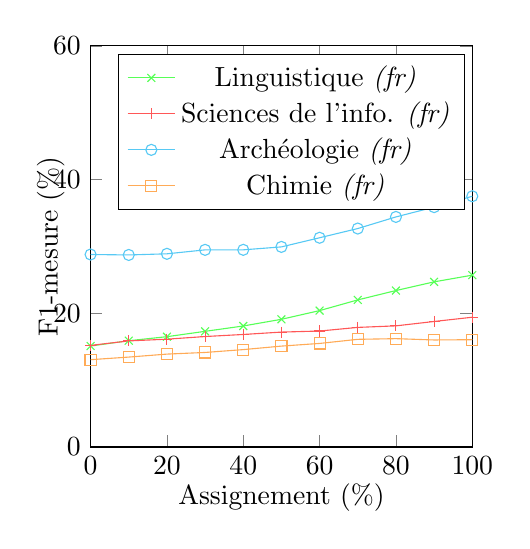
\begin{tikzpicture}
    \pgfkeys{/pgf/number format/.cd, fixed}
    \begin{axis}[x=0.0040\linewidth,
                 xtick={0, 20, ..., 100},
                 xmin=0,
                 xmax=100,
                 xlabel=Assignement (\%),
                 x label style={yshift=.34em},
                 y=0.007\linewidth,
                 ytick={0, 20, ..., 100},
                 ymin=0,
                 ymax=60,
                 ylabel=F1-mesure (\%),
                 y label style={yshift=-1.1em}]
      \addplot[green!66, mark=x] coordinates{
        (0, 15.1)
        (10, 15.9)
        (20, 16.5)
        (30, 17.3)
        (40, 18.1)
        (50, 19.1)
        (60, 20.4)
        (70, 22.0)
        (80, 23.4)
        (90, 24.7)
        (100, 25.7)
      };
      \addplot[red!66, mark=+] coordinates{
        (0, 15.1992)
        (10, 15.8659)
        (20, 16.1269)
        (30, 16.5223)
        (40, 16.8308)
        (50, 17.1875)
        (60, 17.3450)
        (70, 17.8887)
        (80, 18.1184)
        (90, 18.7733)
        (100, 19.4089)
      };
      \addplot[cyan!66, mark=o] coordinates{
        (0, 28.7887)
        (10, 28.7239)
        (20, 28.8927)
        (30, 29.4833)
        (40, 29.4880)
        (50, 29.9271)
        (60, 31.2943)
        (70, 32.6718)
        (80, 34.4101)
        (90, 35.8757)
        (100, 37.5003)
      };
      \addplot[orange!66, mark=square] coordinates{
        (0, 13.0605)
        (10, 13.4498)
        (20, 13.8944)
        (30, 14.1412)
        (40, 14.5673)
        (50, 15.0916)
        (60, 15.4902)
        (70, 16.1045)
        (80, 16.2055)
        (90, 16.0077)
        (100, 16.0506)
      };
      \legend{Linguistique \textit{(fr)}, Sciences de l'info. \textit{(fr)}, Archéologie \textit{(fr)}, Chimie \textit{(fr)}};
    \end{axis}
  \end{tikzpicture}
  \caption{Comportement de TopicCoRank en fonction du taux d'assignement
           \label{fig:assignment_variations}}
\end{figure}



        Enfin, nous réalisons une dernière expérience dans laquelle nous faisons
        varier la valeur du paramètre $\lambda$. Plus sa valeur est élevée, plus
        l'influence de la recommandation interne est forte. La
        figure~\ref{fig:lambda_variations_termith} montre le comportement de
        TopicCoRank\index{topiccorank@TopicCoRank} lorsque nous faisons varier sa valeur de 0 à 1
        avec un pas de 0,1. En accord avec notre hypothèse que sujets\index{sujet@Sujet} et
        termes-clés\index{terme-cle@Terme-clé} du domaine\index{domaine@Domaine} doivent se recommander les uns les autres, les
        résultats\index{resultat@Résultat} montrent que les performances\index{performance@Performance} de TopicCoRank\index{topiccorank@TopicCoRank} se dégradent au
        delà de $\lambda = 0,5$, valeur quasi-optimale.
        \begin{figure}[h!]
  \centering
  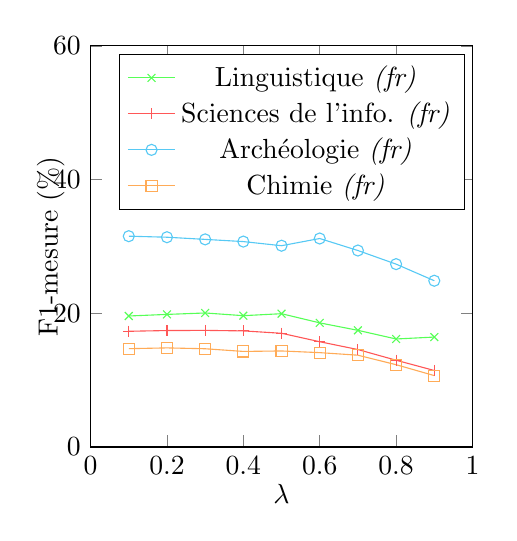
\begin{tikzpicture}
    \pgfkeys{/pgf/number format/.cd, fixed}
    \begin{axis}[x=0.4\linewidth,
                 xtick={0, 0.2, ..., 1.0},
                 xmin=0,
                 xmax=1.0,
                 xlabel=$\lambda$,
                 x label style={yshift=.34em},
                 y=0.007\linewidth,
                 ytick={0, 20, ..., 100},
                 ymin=0,
                 ymax=60,
                 ylabel=F1-mesure (\%),
                 y label style={yshift=-1.1em}]
      \addplot[green!66, mark=x] coordinates{
        (0.1, 19.5942)
        (0.2, 19.8314)
        (0.3, 20.0452)
        (0.4, 19.6420)
        (0.5, 19.9371)
        (0.6, 18.5649)
        (0.7, 17.4499)
        (0.8, 16.1558)
        (0.9, 16.4438)
      };
      \addplot[red!66, mark=+] coordinates{
        (0.1, 17.3100)
        (0.2, 17.4176)
        (0.3, 17.4420)
        (0.4, 17.3653)
        (0.5, 17.0094)
        (0.6, 15.7458)
        (0.7, 14.5758)
        (0.8, 12.9788)
        (0.9, 11.4421)
      };
      \addplot[cyan!66, mark=o] coordinates{
        (0.1, 31.5290)
        (0.2, 31.3748)
        (0.3, 31.0511)
        (0.4, 30.7214)
        (0.5, 30.1052)
        (0.6, 31.1819)
        (0.7, 29.3852)
        (0.8, 27.3498)
        (0.9, 24.8661)
      };
      \addplot[orange!66, mark=square] coordinates{
        (0.1, 14.7061)
        (0.2, 14.8227)
        (0.3, 14.6960)
        (0.4, 14.2947)
        (0.5, 14.3646)
        (0.6, 14.1136)
        (0.7, 13.7321)
        (0.8, 12.3091)
        (0.9, 10.6809)
      };
      \legend{Linguistique \textit{(fr)}, Sciences de l'info. \textit{(fr)}, Archéologie \textit{(fr)}, Chimie \textit{(fr)}};
    \end{axis}
  \end{tikzpicture}
  \caption{Comportement de TopicCoRank en fonction du taux d'assignement
           \label{fig:assignment_variations}}
\end{figure}


      
      \subsubsection{Évaluation de TopicCoRank\index{topiccorank@TopicCoRank} hors domaines\index{domaine@Domaine} de spécialité\index{specialite@Spécialité}}
      \label{subsubsec:main-domain_specific_keyphrase_annotation-supervised_automatic_keyphrase_annotation-evaluation-topiccorank_indepent_domains}
        Nous réalisons ici la même série d'évaluations précédentes, mais hors
        domaines\index{domaine@Domaine} de spécialité\index{specialite@Spécialité}. L'objectif est de déterminer si TopicCoRank\index{topiccorank@TopicCoRank} et
        ses hypothèses, fortement liées à notre étude de l'indexation manuelle
        en domaines\index{domaine@Domaine} de spécialité\index{specialite@Spécialité}, se généralisent à tout type de documents\index{document@Document}.

        Le tableau\index{tableau@Tableau}~\ref{tab:topiccorank-comparison_results_general} montre les
        performances\index{performance@Performance} de TopicCoRank\index{topiccorank@TopicCoRank} hors domaines\index{domaine@Domaine} de spécialité\index{specialite@Spécialité} (\textsc{De}ft,
        SemEval et \textsc{Duc}) comparées à celles des méthodes\index{methode@Méthode} de référence\index{reference@Référence}.
        Les résultats\index{resultat@Résultat} montrent de plus faibles performances\index{performance@Performance} qu'en domaines\index{domaine@Domaine} de
        spécialité\index{specialite@Spécialité}. TopicCoRank\index{topiccorank@TopicCoRank} échoue à améliorer TopicRank\index{topicrank@TopicRank} sur \textsc{De}ft,
        l'améliore légèrement sur SemEval et l'améliore significativement sur
        \textsc{Duc}, pour lequel nous utilisons des graphes\index{graphe@Graphe} de domaine\index{domaine@Domaine} très
        centrés sur le sujet\index{sujet@Sujet} d'actualité de chaque document\index{document@Document} de test.
        Contrairement à ce que nous observons en domaines\index{domaine@Domaine} de spécialité\index{specialite@Spécialité}, c'est
        TopicCoRank\index{topiccorank@TopicCoRank} qui est majoritairement le plus performant et c'est sa
        variante TopicCoRank\index{topiccorank@TopicCoRank}$_\textnormal{assign.}$ qui est la moins
        performante. L'explication tient à la nature des termes-clés\index{terme-cle@Terme-clé} de
        référence\index{reference@Référence} de \textsc{De}ft et SemEval. Ceux-ci n'ont pas été produit à
        l'aide d'un vocabulaire\index{vocabulaire@Vocabulaire} contrôlé et les cinq principes sur lesquels nous
        fondons nos hypothèses ne sont pas respectés. La contrainte de
        conformité n'étant pas respectée, la nécessité de l'assignement n'est
        pas garantie~; la contrainte d'homogénéité n'étant pas respectée non
        plus, le graphe\index{graphe@Graphe} de domaine\index{domaine@Domaine} que nous construisons contient des
        termes-clés\index{terme-cle@Terme-clé} de référence\index{reference@Référence} redondants\index{redondant@Redondant}. La redondance des termes-clés\index{terme-cle@Terme-clé} de
        référence\index{reference@Référence} requiert une étape de normalisation. Celle-ci peut s'effectuer
        à l'aide de notre méthode\index{methode@Méthode} de groupement en sujets\index{sujet@Sujet}.
        \begin{table}
          \centering
          %\resizebox{\linewidth}{!}{
            \begin{tabular}{l|ccc|ccc|ccc}
              \toprule
              \multirow{2}{*}{\textbf{Méthode}} & \multicolumn{3}{c|}{\textbf{\textsc{De}ft} \textit{(fr)}} & \multicolumn{3}{c|}{\textbf{SemEval} \textit{(en)}} & \multicolumn{3}{c}{\textbf{\textsc{Duc}} \textit{(en)}}\\
              \cline{2-10}
              & P & R & F & P & R & F & P & R & F\\
              \hline
              \textsc{Tf-Idf} & 10,4 & 19,1 & 13,3 & 13,6 & $~~$9,3 & 10,9 & 24,9 & 32,1 & 27,7$^{~~}$\\
              TopicRank & \textbf{11,9} & \textbf{21,5} & \textbf{14,9} & 16,6 & 11,5 & 13,5 & 17,9 & 23,7 & 20,1$^{~~}$\\
              KEA++ & & & & & & & & &\\
              \overtabline
              \hline
              TopicCoRank$_\textnormal{extr.}$ & 10,1 & 19,1 & 13,0 & 17,4 & 12,3 & 14,3 & 24,6 & 35,5 & 27,2$^{~~}$\\
              TopicCoRank$_\textnormal{assign.}$ & $~~$6,8 & 12,8 & $~~$8,7 & 11,8 & $~~$8,4 & $~~$9,7 & 25,8 & 33,1 & 28,6$^{~~}$\\
              \hline
              TopicCoRank & $~~$8,7 & 16,2 & 11,2 & \textbf{17,6} & \textbf{12,5} & \textbf{14,5} & \textbf{28,2} & \textbf{36,3} & \textbf{31,3}$^\dagger$\\
              \bottomrule
            \end{tabular}
          %}
        \caption[
          Résultat de l'extraction de dix termes-clés avec \textsc{Tf-Idf},
          TopicRank, \textsc{Kea++}, TopicCoRank$_\textnormal{\textit{extr.}}$,
          TopicCoRank$_\textnormal{\textit{assign.}}$ et TopicCoRank appliqués à
          \textsc{De}ft, SemEval et \textsc{Duc}
        ]{
          Résultat de l'extraction de dix termes-clés avec \textsc{Tf-Idf},
          TopicRank, \textsc{Kea++}, TopicCoRank$_\textnormal{\textit{extr.}}$,
          TopicCoRank$_\textnormal{\textit{assign.}}$ et TopicCoRank appliqués à
          \textsc{De}ft, SemEval et \textsc{Duc}. $\dagger$ indique une
          amélioration significative vis-à-vis des méthodes de référence, à
          0,001 pour le t-test de Student.
          \label{tab:topiccorank-comparison_results_general}}
        \end{table}

        La figure~\ref{fig:topiccorank-pr_curves_general} permet de comparer le
        comportement respectif des méthodes\index{methode@Méthode} de référence\index{reference@Référence}, de TopicCoRank\index{topiccorank@TopicCoRank} et de
        ses variantes. Contrairement aux domaines\index{domaine@Domaine} de spécialité\index{specialite@Spécialité}, où TopicCoRank\index{topiccorank@TopicCoRank}
        et ses variantes dominent les méthodes\index{methode@Méthode} de référence\index{reference@Référence}, nous observons ici
        qu'aucune méthode\index{methode@Méthode} dominante ne se dégage et, sauf sur \textsc{Duc}, il
        est difficile de statuer sur l'apport de TopicCoRank\index{topiccorank@TopicCoRank} à TopicRank\index{topicrank@TopicRank}. Par
        ailleurs, le rappel maximal atteint par TopicCoRank\index{topiccorank@TopicCoRank} n'excède, dans la
        plupart des cas, pas celui de \textsc{Tf-Idf\index{tf-idf@TF-IDF}}. TopicCoRank\index{topiccorank@TopicCoRank} étant capable
        d'assigner des termes-clés\index{terme-cle@Terme-clé} qui n'occurrent pas dans le document\index{document@Document}, son
        rappel maximal devrait être plus grand. Il existe deux raisons à ce
        problème. La première est aussi valable pour TopicRank\index{topicrank@TopicRank}. Comme les
        termes-clés\index{terme-cle@Terme-clé} candidats sont groupés en sujets\index{sujet@Sujet} et qu'un seul d'entre eux
        est extrait par sujet\index{sujet@Sujet}, si un terme-clé\index{terme-cle@Terme-clé} erroné est extrait d'un sujet\index{sujet@Sujet}
        contenant un terme-clé\index{terme-cle@Terme-clé} correct, alors le rappel maximal observable est
        plus faible que celui de \textsc{Tf-Idf\index{tf-idf@TF-IDF}}, qui peut extraire tous les
        candidats lorsque nous le lui demandons. La seconde raison nous
        intéresse particulièrement, car elle n'est pas observable en domaines\index{domaine@Domaine} de
        spécialité\index{specialite@Spécialité}. En effet, le problème est aussi due à l'inconsistance des
        données d'entraînement pour représenter un \og{}domaine\index{domaine@Domaine}\fg{} de manière
        homogène et conforme à son vocabulaire\index{vocabulaire@Vocabulaire}. Les termes-clés\index{terme-cle@Terme-clé} employés dans
        les documents\index{document@Document} d'entraînement ne sont pas les mêmes que ceux employés
        pour les documents\index{document@Document} de test et l'assignement ne fonctionne donc pas.
        \begin{figure}[h!]
  \subfigure[\textsc{De}ft \textit{(fr)}]{
    \begin{tikzpicture}
      \pgfkeys{/pgf/number format/.cd, fixed}
      \begin{axis}[x=0.0057\linewidth,
                   xtick={0, 20, 40, ..., 100},
                   xmin=0,
                   xmax=60,
                   xlabel=rappel (\%),
                   x label style={yshift=.34em},
                   y=0.0057\linewidth,
                   ytick={0, 20, ..., 100},
                   ymin=0,
                   ymax=60,
                   ylabel=précision (\%),
                   y label style={yshift=-1.1em}]
        \addplot [green!66, mark=x] file {input/figure/data/deft_tfidf.csv};
        \addplot [red!66, mark=+] file {input/figure/data/deft_topicrank.csv};
        \addplot [orange!66, mark=square] file {input/figure/data/deft_topiccorank_extr.csv};
        \addplot [black!66, mark=triangle] file {input/figure/data/deft_topiccorank_assign.csv};
        \addplot [gray!66, mark=diamond] file {input/figure/data/deft_topiccorank.csv};
        %%%%%%%%%%%%%%%%%%%%%%%%%%%%%%%%%%%%%%%%%%%%%%%%%%%%%%%%%%%%%%%%%%%%%%%%
        \addplot [dotted, domain=35:100] {(50 * x) / ((2 * x) - 50)};
        \addplot [dotted, domain=25:100] {(40 * x) / ((2 * x) - 40)};
        \addplot [dotted, domain=15:100] {(30 * x) / ((2 * x) - 30)};
        \addplot [dotted, domain=10:100] {(20 * x) / ((2 * x) - 20)};
        \addplot [dotted, domain=5:100] {(10 * x) / ((2 * x) - 10)};
      \end{axis}
      \node at (4.85,3.6) [anchor=east] {\footnotesize{F=50,0}};
      \node at (4.85,2.6) [anchor=east] {\footnotesize{F=40,0}};
      \node at (4.85,1.8) [anchor=east] {\footnotesize{F=30,0}};
      \node at (4.85,1.15) [anchor=east] {\footnotesize{F=20,0}};
      \node at (4.85,0.6) [anchor=east] {\footnotesize{F=10,0}};
    \end{tikzpicture}
  }
  \subfigure[Semeval \textit{(en)}]{
    \begin{tikzpicture}
      \pgfkeys{/pgf/number format/.cd, fixed}
      \begin{axis}[x=0.0057\linewidth,
                   xtick={0, 20, 40, ..., 100},
                   xmin=0,
                   xmax=60,
                   xlabel=rappel (\%),
                   x label style={yshift=.34em},
                   y=0.0057\linewidth,
                   ytick={0, 20, ..., 100},
                   ymin=0,
                   ymax=60,
                   ylabel=précision (\%),
                   y label style={yshift=-1.1em}]
        \addplot [green!66, mark=x] file {input/figure/data/semeval_tfidf.csv};
        \addplot [red!66, mark=+] file {input/figure/data/semeval_topicrank.csv};
        \addplot [orange!66, mark=square] file {input/figure/data/semeval_topiccorank_extr.csv};
        \addplot [black!66, mark=triangle] file {input/figure/data/semeval_topiccorank_assign.csv};
        \addplot [gray!66, mark=diamond] file {input/figure/data/semeval_topiccorank.csv};
        %%%%%%%%%%%%%%%%%%%%%%%%%%%%%%%%%%%%%%%%%%%%%%%%%%%%%%%%%%%%%%%%%%%%%%%%
        %\addplot [dotted, domain=35:100] {(50 * x) / ((2 * x) - 50)};
        %\addplot [dotted, domain=25:100] {(40 * x) / ((2 * x) - 40)};
        \addplot [dotted, domain=15:100] {(30 * x) / ((2 * x) - 30)};
        \addplot [dotted, domain=10:100] {(20 * x) / ((2 * x) - 20)};
        \addplot [dotted, domain=5:100] {(10 * x) / ((2 * x) - 10)};
        %%%%%%%%%%%%%%%%%%%%%%%%%%%%%%%%%%%%%%%%%%%%%%%%%%%%%%%%%%%%%%%%%%%%%%%%
        \legend{\textsc{Tf-Idf}, TopicRank, TopicCoRank$_\textnormal{extr.}$,
                TopicCoRank$_\textnormal{assign.}$, TopicCoRank};        
      \end{axis}
      %\node at (4.85,3.6) [anchor=east] {\footnotesize{F=50,0}};
      %\node at (4.85,2.6) [anchor=east] {\footnotesize{F=40,0}};
      \node at (4.85,1.8) [anchor=east] {\footnotesize{F=30,0}};
      \node at (4.85,1.15) [anchor=east] {\footnotesize{F=20,0}};
      \node at (4.85,0.6) [anchor=east] {\footnotesize{F=10,0}};
    \end{tikzpicture}
  }
  \subfigure[\textsc{Duc} \textit{(en)}]{
    \begin{tikzpicture}
      \pgfkeys{/pgf/number format/.cd, fixed}
      \begin{axis}[x=0.0057\linewidth,
                   xtick={0, 20, 40, ..., 100},
                   xmin=0,
                   xmax=60,
                   xlabel=rappel (\%),
                   x label style={yshift=.34em},
                   y=0.0057\linewidth,
                   ytick={0, 20, ..., 100},
                   ymin=0,
                   ymax=60,
                   ylabel=précision (\%),
                   y label style={yshift=-1.1em}]
        \addplot [green!66, mark=x] file {input/figure/data/duc_tfidf.csv};
        \addplot [red!66, mark=+] file {input/figure/data/duc_topicrank.csv};
        \addplot [orange!66, mark=square] file {input/figure/data/duc_topiccorank_extr.csv};
        \addplot [black!66, mark=triangle] file {input/figure/data/duc_topiccorank_assign.csv};
        \addplot [gray!66, mark=diamond] file {input/figure/data/duc_topiccorank.csv};
        %%%%%%%%%%%%%%%%%%%%%%%%%%%%%%%%%%%%%%%%%%%%%%%%%%%%%%%%%%%%%%%%%%%%%%%%
        \addplot [dotted, domain=35:100] {(50 * x) / ((2 * x) - 50)};
        \addplot [dotted, domain=25:100] {(40 * x) / ((2 * x) - 40)};
        \addplot [dotted, domain=15:100] {(30 * x) / ((2 * x) - 30)};
        \addplot [dotted, domain=10:100] {(20 * x) / ((2 * x) - 20)};
        \addplot [dotted, domain=5:100] {(10 * x) / ((2 * x) - 10)};
      \end{axis}
      \node at (4.85,3.6) [anchor=east] {\footnotesize{F=50,0}};
      \node at (4.85,2.6) [anchor=east] {\footnotesize{F=40,0}};
      \node at (4.85,1.8) [anchor=east] {\footnotesize{F=30,0}};
      \node at (4.85,1.15) [anchor=east] {\footnotesize{F=20,0}};
      \node at (4.85,0.6) [anchor=east] {\footnotesize{F=10,0}};
    \end{tikzpicture}
  }
  \caption{Courbes de rappel-précision de \textsc{Tf-Idf}, TopicRank,
           TopicCoRank$_\textnormal{extr.}$, TopicCoRank$_\textnormal{assign.}$
           et TopicCoRank appliqués à \textsc{De}ft, SemEval et \textsc{Duc}
           \label{fig:topiccorank-pr_curves}}
\end{figure}



        Comme pour l'évaluation en domaines\index{domaine@Domaine} de spécialité\index{specialite@Spécialité}, le
        tableau\index{tableau@Tableau}~\ref{tab:assignment_ratio_general} reporte les taux d'extraction
        et d'assignement réalisés par TopicCoRank\index{topiccorank@TopicCoRank} sur \textsc{De}ft, SemEval et
        \textsc{Duc}. Ceux-ci montrent aussi que les deux catégories
        d'indexation sont réalisées conjointement, cette fois-ci sans
        prédominance de l'une face à l'autre.
        \begin{table}[h]
          \centering
          \begin{tabular}{l|c|c}
              \toprule
              & Extraction (\%) & Assignement (\%)\\
              \hline
              \textsc{De}ft \textit{(fr)} & 48,4 & 51,6\\
              SemEval \textit{(en)} & 61,4 & 38,6\\
              \textsc{Duc} \textit{(en)} & 46,9 & 53,1\\
              \bottomrule
          \end{tabular}
          \caption{Taux moyens d'extraction et d'assignement réalisés par
                   TopicCoRank sur \textsc{De}ft, SemEval et \textsc{Duc}
                   \label{tab:assignment_ratio_general}}
        \end{table}

        La figure~\ref{fig:assignment_variations_general} montrent les
        performances\index{performance@Performance} de TopicCoRank\index{topiccorank@TopicCoRank} lorsque nous forçons le taux d'assignement,
        de 0~\% à 100~\% avec un pas de 10~\%. Contrairement à la courbe de
        performances\index{performance@Performance} en domaines\index{domaine@Domaine} de spécialité\index{specialite@Spécialité}, celle de TopicCoRank\index{topiccorank@TopicCoRank} hors
        domaines\index{domaine@Domaine} de spécialité\index{specialite@Spécialité} est croissante puis décroissante pour \text{Duc}
        et est principalement décroissante pour \textsc{De}ft et SemEval. Cela signifie que
        l'ordonnancement des termes-clés\index{terme-cle@Terme-clé} du domaine\index{domaine@Domaine} est moins efficace hors
        domaines\index{domaine@Domaine} de spécialité\index{specialite@Spécialité}. Il est toutefois intéressant de noter que, sur
        \textsc{Duc}, le taux d'assignement effectué par TopicCoRank\index{topiccorank@TopicCoRank} sans que
        nous ne le forcions est proche de sa valeur optimal.
        \begin{figure}[h!]
  \centering
  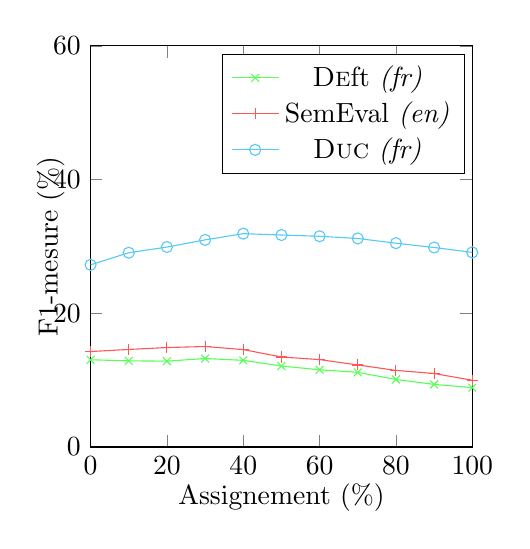
\begin{tikzpicture}
    \pgfkeys{/pgf/number format/.cd, fixed}
    \begin{axis}[x=0.0040\linewidth,
                 xtick={0, 20, ..., 100},
                 xmin=0,
                 xmax=100,
                 xlabel=Assignement (\%),
                 x label style={yshift=.34em},
                 y=0.007\linewidth,
                 ytick={0, 20, ..., 100},
                 ymin=0,
                 ymax=60,
                 ylabel=F1-mesure (\%),
                 y label style={yshift=-1.1em}]
      \addplot[green!66, mark=x] coordinates{
        (0, 13.0470)
        (10, 12.8868)
        (20, 12.8409)
        (30, 13.2342)
        (40, 12.9643)
        (50, 12.1117)
        (60, 11.5492)
        (70, 11.1649)
        (80, 10.1043)
        (90, 9.3643)
        (100, 8.8794)
      };
      \addplot[red!66, mark=+] coordinates{
        (0, 14.2790)
        (10, 14.5905)
        (20, 14.8776)
        (30, 15.0293)
        (40, 14.5713)
        (50, 13.4616)
        (60, 13.0731)
        (70, 12.2721)
        (80, 11.4582)
        (90, 10.9929)
        (100, 9.9841)
      };
      \addplot[cyan!66, mark=o] coordinates{
        (0, 27.2447)
        (10, 29.0553)
        (20, 29.9039)
        (30, 30.9763)
        (40, 31.9071)
        (50, 31.7050)
        (60, 31.5150)
        (70, 31.1887)
        (80, 30.4816)
        (90, 29.8382)
        (100, 29.1068)
      };
      \legend{\textsc{De}ft \textit{(fr)}, SemEval \textit{(en)}, \textsc{Duc} \textit{(fr)}};
    \end{axis}
  \end{tikzpicture}
  \caption{Comportement de TopicCoRank en fonction du taux d'assignement
           \label{fig:assignment_variations}}
\end{figure}



        La figure~\ref{fig:lambda_variations_general} montre le comportement de
        TopicCoRank\index{topiccorank@TopicCoRank} lorsque nous faisons varier la valeur de $\lambda$ de 0 à 1
        avec un pas de 0,1. Sur \textsc{Duc}, comme en domaines\index{domaine@Domaine} des spécialité\index{specialite@Spécialité},
        l'indexation par termes-clés\index{terme-cle@Terme-clé} est meilleure\index{meilleur@Meilleur} lorsque l'ordonnancement est
        fortement influencé par la recommandation externe que lorsqu'il ne l'est
        pas. Sur \textsc{De}ft et SemEval, c'est l'inverse. Comme observé précédemment, les données
        d'entraînement sont telles que le graphe\index{graphe@Graphe} du domaine\index{domaine@Domaine} est moins utile pour
        ces données.
        \begin{figure}[t]
  \centering
  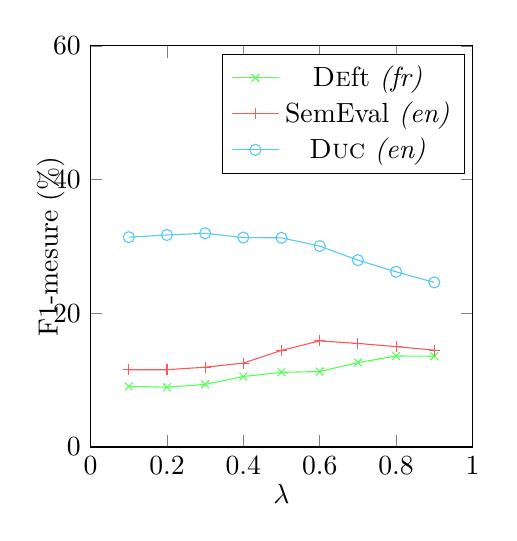
\begin{tikzpicture}
    \pgfkeys{/pgf/number format/.cd, fixed}
    \begin{axis}[x=0.4\linewidth,
                 xtick={0, 0.2, ..., 1.0},
                 xmin=0,
                 xmax=1.0,
                 xlabel=$\lambda$,
                 x label style={yshift=.34em},
                 y=0.007\linewidth,
                 ytick={0, 20, ..., 100},
                 ymin=0,
                 ymax=60,
                 ylabel=F1-mesure (\%),
                 y label style={yshift=-1.1em}]
      \addplot[green!66, mark=x] coordinates{
        (0.1, 9.0736)
        (0.2, 8.9392)
        (0.3, 9.3693)
        (0.4, 10.5436)
        (0.5, 11.1626)
        (0.6, 11.2902)
        (0.7, 12.6269)
        (0.8, 13.6109)
        (0.9, 13.5765)
      };
      \addplot[red!66, mark=+] coordinates{
        (0.1, 11.5509)
        (0.2, 11.5618)
        (0.3, 11.9382)
        (0.4, 12.5558)
        (0.5, 14.4539)
        (0.6, 15.8712)
        (0.7, 15.4920)
        (0.8, 15.0102)
        (0.9, 14.4863)
      };
      \addplot[cyan!66, mark=o] coordinates{
        (0.1, 31.3789)
        (0.2, 31.7112)
        (0.3, 31.9601)
        (0.4, 31.3222)
        (0.5, 31.2842)
        (0.6, 30.0481)
        (0.7, 27.9426)
        (0.8, 26.1973)
        (0.9, 24.6206)
      };
      \legend{\textsc{De}ft \textit{(fr)}, SemEval \textit{(en)}, \textsc{Duc} \textit{(en)}};
    \end{axis}
  \end{tikzpicture}
  \caption{Performance de TopicCoRank, appliqué à \textsc{De}ft, SemEval et
           \textsc{Duc}, lorsque le paramètre $\lambda$ varie
           \label{fig:lambda_variations_general}}
\end{figure}



    \subsection{Analyse des sorties de TopicCoRank\index{topiccorank@TopicCoRank}}
    \label{subsec:main-domain_specific_keyphrase_annotation-supervised_automatic_keyphrase_annotation-error_analysis}
      Dans cette section, nous analysons les termes-clés\index{terme-cle@Terme-clé} corrects (vrais
      positifs) et incorrects (faux positifs) issus du graphe\index{graphe@Graphe} du domaine\index{domaine@Domaine} des
      collections Termith.

      \subsubsection{Analyse des vrais positifs}
      \label{subsec:main-domain_specific_keyphrase_annotation-supervised_automatic_keyphrase_annotation-error_analysis-true_positives}
        Parmi les termes-clés\index{terme-cle@Terme-clé} assignés, ceux qui sont corrects sont en grande
        partie présents dans le contenu du document\index{document@Document}. Ils sont directement
        connectés aux sujets\index{sujet@Sujet} du document\index{document@Document} et leur importance\index{importance@Importance} respective évolue de
        manière similaire. Il est fréquent qu'un terme-clé\index{terme-cle@Terme-clé} candidat d'un sujet\index{sujet@Sujet}
        soit extrait en même temps qu'un terme-clé\index{terme-cle@Terme-clé} de référence\index{reference@Référence} du domaine\index{domaine@Domaine}
        connecté à ce sujet\index{sujet@Sujet}. Dans cette situation, nous distinguons deux cas de
        figure~: un seul terme-clé\index{terme-cle@Terme-clé} est produit, car le terme-clé\index{terme-cle@Terme-clé} extrait et
        celui assigné sont les mêmes~; deux termes-clés\index{terme-cle@Terme-clé} corrects complémentaires
        sont produits, car le terme-clé\index{terme-cle@Terme-clé} extrait et celui assigné ne sont pas les
        mêmes.
        
        Il est plus difficile pour les termes-clés\index{terme-cle@Terme-clé} de référence\index{reference@Référence} du domaine\index{domaine@Domaine}
        connectés indirectement aux sujets\index{sujet@Sujet} du document\index{document@Document} d'émerger. Nous observons
        toutefois l'émergence de quelques termes-clés\index{terme-cle@Terme-clé} absents du documents\index{document@Document}
        (par exemple\index{exemple@Exemple}, \og{}analyse du discours\fg{} en linguistique et
        les noms\index{nom@Nom} de composés \og{}composé aliphatique\fg{}, \og{}composé
        benzénique\fg{}, etc. en chimie), et de termes-clés\index{terme-cle@Terme-clé} génériques (par
        exemple\index{exemple@Exemple} \og{}français\fg{} en linguistique, ou encore \og{}Europe\fg{}
        en archéologie). Nous observons dans les données Termith des cadres
        d'études très récurrents (par exemple\index{exemple@Exemple}, la langue française, en
        linguistique, ou des fouilles de sites européens, en archéologie) et, de
        ce fait, certains termes-clés\index{terme-cle@Terme-clé} génériques sont très fréquemment utilisés
        (\og{}français\fg{} apparaît dans 48,9~\% des documents\index{document@Document} de linguistique
        et \og{}Europe\fg{} apparaît dans 52,5~\% des documents\index{document@Document} d'archéologie).

      \subsubsection{Analyse des faux positifs}
      \label{subsec:main-domain_specific_keyphrase_annotation-supervised_automatic_keyphrase_annotation-error_analysis-false_positives}
        Les termes-clés\index{terme-cle@Terme-clé} génériques évoqués dans l'analyse des vrais positifs
        sont aussi sources d'erreurs. En effet, comme ils sont associés à un
        nombre\index{nombre@Nombre} conséquent de documents\index{document@Document} d'entraînement, ils sont connectés à
        beaucoup d'autres termes-clés\index{terme-cle@Terme-clé} du domaine\index{domaine@Domaine} et gagnent donc de l'importance\index{importance@Importance}
        quelque soit le document\index{document@Document}. Pour l'exemple\index{exemple@Exemple} du terme-clé\index{terme-cle@Terme-clé} \og{}français\fg{}
        en linguistique, nous observons des documents\index{document@Document} qui traitent de l'arabe
        mais, parce que les termes techniques employés sont les mêmes
        (\og{}syntaxe\fg{}, \og{}sémantique\fg{}, etc.), \og{}français\fg{} est
        assigné.

        Enfin, nous observons quelques problèmes liés à la présence de
        termes-clés\index{terme-cle@Terme-clé} de référence\index{reference@Référence} redondants\index{redondant@Redondant}, c'est-à-dire des synonymes. C'est
        le cas, par exemple\index{exemple@Exemple}, du terme-clé\index{terme-cle@Terme-clé} \og{}rite funéraire\fg{}, qui fait
        parti du vocabulaire\index{vocabulaire@Vocabulaire} contrôlé d'archéologie, et qui est parfois remplacé
        par le terme-clé\index{terme-cle@Terme-clé} \og{}pratique funéraire\fg{}, qui ne fait pas partie du
        vocabulaire\index{vocabulaire@Vocabulaire} contrôlé d'archéologie. TopicCoRank\index{topiccorank@TopicCoRank} échoue parfois parce
        qu'il a assigné l'un alors que c'était l'autre qu'il fallait trouver.

    \subsection{Bilan}
    \label{subsec:main-domain_specific_keyphrase_annotation-supervised_automatic_keyphrase_annotation-conclusion}
      Nous avons présenté TopicCoRank\index{topiccorank@TopicCoRank}, une extension de la méthode\index{methode@Méthode} TopicRank\index{topicrank@TopicRank}.
      Proposée dans le but de simuler le comportement d'un indexeur
      professionnel, cette extension apporte à TopicRank\index{topicrank@TopicRank} la capacité à assigner
      des termes-clés\index{terme-cle@Terme-clé}. Pour ce faire, TopicCoRank\index{topiccorank@TopicCoRank} utilise les termes-clés\index{terme-cle@Terme-clé} de
      référence\index{reference@Référence} des documents\index{document@Document} d'entraînement comme vocabulaire\index{vocabulaire@Vocabulaire} contrôlé, crée un
      graphe\index{graphe@Graphe} du domaine\index{domaine@Domaine} à partir de ces termes-clés\index{terme-cle@Terme-clé}, puis unifie ce
      graphe\index{graphe@Graphe} au graphe\index{graphe@Graphe} de sujets\index{sujet@Sujet} de TopicRank\index{topicrank@TopicRank}. Termes-clés\index{terme-cle@Terme-clé} du domaines\index{domaine@Domaine} et sujets\index{sujet@Sujet}
      du document\index{document@Document} sont ensuite ordonnés conjointement pour extraire des
      termes-clés\index{terme-cle@Terme-clé} à partir des sujets\index{sujet@Sujet} et en assigner à partir des termes-clés\index{terme-cle@Terme-clé} du
      domaine\index{domaine@Domaine}.

      Les résultats\index{resultat@Résultat} de l'évaluation de TopicCoRank\index{topiccorank@TopicCoRank} en domaines\index{domaine@Domaine} de spécialité\index{specialite@Spécialité}
      montrent une amélioration significative vis-à-vis de l'état de l'art. Ceux
      hors domaines\index{domaine@Domaine} de spécialité\index{specialite@Spécialité} sont moins probants. Les hypothèses que nous
      faisons en proposant TopicCoRank\index{topiccorank@TopicCoRank} sont fondées sur une étude de
      l'indexation manuelle en domaines\index{domaine@Domaine} de spécialité\index{specialite@Spécialité} qui ne sont pas
      directement généralisables à tout type de documents\index{document@Document}.

  %-----------------------------------------------------------------------------

  \section{Évaluation manuelle\index{evaluation manuelle@Évaluation manuelle} en domaines\index{domaine@Domaine} de spécialité\index{specialite@Spécialité}}
  \label{sec:main-domain_specific_keyphrase_annotation-manual_evaluation}
    L'évaluation manuelle\index{evaluation manuelle@Évaluation manuelle} des méthodes\index{methode@Méthode} d'indexation par termes-clés\index{terme-cle@Terme-clé} consiste à
    faire valider par un ou plusieurs évaluateurs humains les termes-clés\index{terme-cle@Terme-clé}
    proposés par une méthodes\index{methode@Méthode} automatique. Parce qu'elle est coûteuse, cette
    évaluation est quasi-systématiquement remplacée par une évaluation
    automatique, d'après le paradigme de l'évaluation \og{}à la Crandield\fg{},
    comme nous l'avons fait dans nos travaux. Néanmoins, ce paradigme
    d'évaluation n'est pas adapté à la tâche d'indexation par termes-clés\index{terme-cle@Terme-clé}, car
    il ne considère qu'une seule et unique réponse exacte, c'est-à-dire un seul
    et unique ensemble\index{ensemble@Ensemble} correct de termes-clés\index{terme-cle@Terme-clé}, alors que certaines variantes
    d'ensembles\index{ensemble@Ensemble} de termes-clés\index{terme-cle@Terme-clé} sont acceptables (par exemple\index{exemple@Exemple}, un ensemble\index{ensemble@Ensemble} avec
    \og{}rite funéraire\fg{} et une variante avec \og{}pratique funéraire\fg{}).
    Ayant à notre disposition des indexeurs professionnels de l'Inist, nous
    réalisons donc une campagne d'évaluation manuelle\index{evaluation manuelle@Évaluation manuelle}.

    Dans la suite, nous présentons le protocole d'évaluation et les métriques
    que nous avons proposé, puis nous analysons les premiers résultats\index{resultat@Résultat} de la
    campagne d'évaluation manuelle\index{evaluation manuelle@Évaluation manuelle} de TopicRank\index{topicrank@TopicRank}, TopicCoRank\index{topiccorank@TopicCoRank} et de deux méthodes\index{methode@Méthode} de référence\index{reference@Référence} en
    domaine\index{domaine@Domaine} de spécialité\index{specialite@Spécialité} avec la collection de linguistique Termith.

    \subsection{Protocole d'évaluation manuelle\index{evaluation manuelle@Évaluation manuelle}}
    \label{subsec:main-automatic_evaluation_of_keyphrase_annotation-methodology-evaluation_protocol}
      L'évaluation manuelle\index{evaluation manuelle@Évaluation manuelle} concerne dix termes-clés\index{terme-cle@Terme-clé} extraits/assignés par
      chaque méthode\index{methode@Méthode} d'indexation par termes-clés\index{terme-cle@Terme-clé}. Le protocole que nous
      proposons permet d'évaluer deux aspects de l'indexation automatique\index{indexation automatique@Indexation automatique} par
      termes-clés\index{terme-cle@Terme-clé}~:
      \begin{enumerate}
        \item{Pertinence (validité)~: chaque terme-clé\index{terme-cle@Terme-clé} fourni par la méthode\index{methode@Méthode}
              d'indexation automatique\index{indexation automatique@Indexation automatique} par termes-clés\index{terme-cle@Terme-clé} est-il important pour la
              compréhension du contenu principal du document\index{document@Document}~?}
        \item{Silence~: quel est le degré d'importance\index{importance@Importance} des informations perdues
              entre les termes-clés\index{terme-cle@Terme-clé} de référence\index{reference@Référence} et les termes-clés\index{terme-cle@Terme-clé} fournis par
              la méthode\index{methode@Méthode} d'indexation automatique\index{indexation automatique@Indexation automatique} par termes-clés\index{terme-cle@Terme-clé}~?}
      \end{enumerate}
      L'évaluation de la pertinence s'intéresse au même aspect que l'évaluation
      automatique~: le nombre\index{nombre@Nombre} de termes-clés\index{terme-cle@Terme-clé} corrects doit être maximisé et le
      nombre\index{nombre@Nombre} d'erreurs minimisé pour obtenir la meilleure\index{meilleur@Meilleur} performance\index{performance@Performance}.
      L'évaluation du silence s'intéresse à un aspect qui lui est propre. Elle a
      une dimension plus sémantique~: les termes-clés\index{terme-cle@Terme-clé} corrects dont
      l'information est la plus capitale pour la compréhension du contenu
      principal du document\index{document@Document} doivent être priorisés pour obtenir la meilleure\index{meilleur@Meilleur}
      performance\index{performance@Performance}.

      Afin de minimiser les problèmes d'ambiguïté et de subjectivité de certains
      cas de figure, la pertinence et le silence sont évalués sur une échelle à
      trois valeurs~: une valeur représentant le succès, une autre l'échec et
      une dernière le cas intermédiaire.

      \subsubsection{Évaluation de la pertinence}
      \label{subsubsec:main-automatic_evaluation_of_keyphrase_annotation-methodology-evaluation_protocol-relevancy}
        Pour évaluer la pertinence d'un terme-clé\index{terme-cle@Terme-clé} fourni par une méthode\index{methode@Méthode}
        d'indexation par termes-clés\index{terme-cle@Terme-clé}, l'évaluateur doit lui attribuer un score\index{score@Score}
        sur une échelle de 0 à 2. Ce score\index{score@Score} distingue les termes-clés\index{terme-cle@Terme-clé} incorrects
        (0), les termes-clés\index{terme-cle@Terme-clé} corrects (2) et les variantes de ces derniers (1).

        Pour permettre une étude précise de cette évaluation, les indexeurs
        professionnels doi\-vent indiquer la forme préférée des termes-clés\index{terme-cle@Terme-clé}
        auxquels ils donnent un score\index{score@Score} de 1 (variantes). Une variante peut faire
        référence\index{reference@Référence} à deux catégories de formes préférées, qui induisent deux
        raisonnements~:
        \begin{itemize}
          \item{variante d'un terme-clé\index{terme-cle@Terme-clé} déjà fourni (score\index{score@Score} de
                2)~$\Rightarrow$~la méthode\index{methode@Méthode} d'indexation par termes-clés\index{terme-cle@Terme-clé} fourni
                des termes-clés\index{terme-cle@Terme-clé} redondants\index{redondant@Redondant} (voir la figure~\ref{fig:idefix})~;}
          \item{variante d'un terme-clé\index{terme-cle@Terme-clé} non fourni mais présent dans le
                texte~$\Rightarrow$~la méthode\index{methode@Méthode} d'indexation par termes-clés\index{terme-cle@Terme-clé}
                identifie correctement les sujets\index{sujet@Sujet} importants du document\index{document@Document}, mais
                peine à trouver la forme la plus appropriée pour les
                représenter.}
        \end{itemize}

        Lorsque la forme préférée n'est pas présente dans le document\index{document@Document}, nous
        estimons que la méthode\index{methode@Méthode} d'indexation a fourni un terme-clé\index{terme-cle@Terme-clé} correct,
        auquel cas il se voit attribuer le score\index{score@Score} de 2 (voir la
        figure~\ref{fig:idefix}). Les formes variantes résultant d'un accord en
        nombre\index{nombre@Nombre} (pluriel) obtiennent aussi un score\index{score@Score} de 2, lorsque la forme
        normalisée (singulier) ne se trouve pas parmi les termes-clés\index{terme-cle@Terme-clé} fournis.
        \begin{figure}
          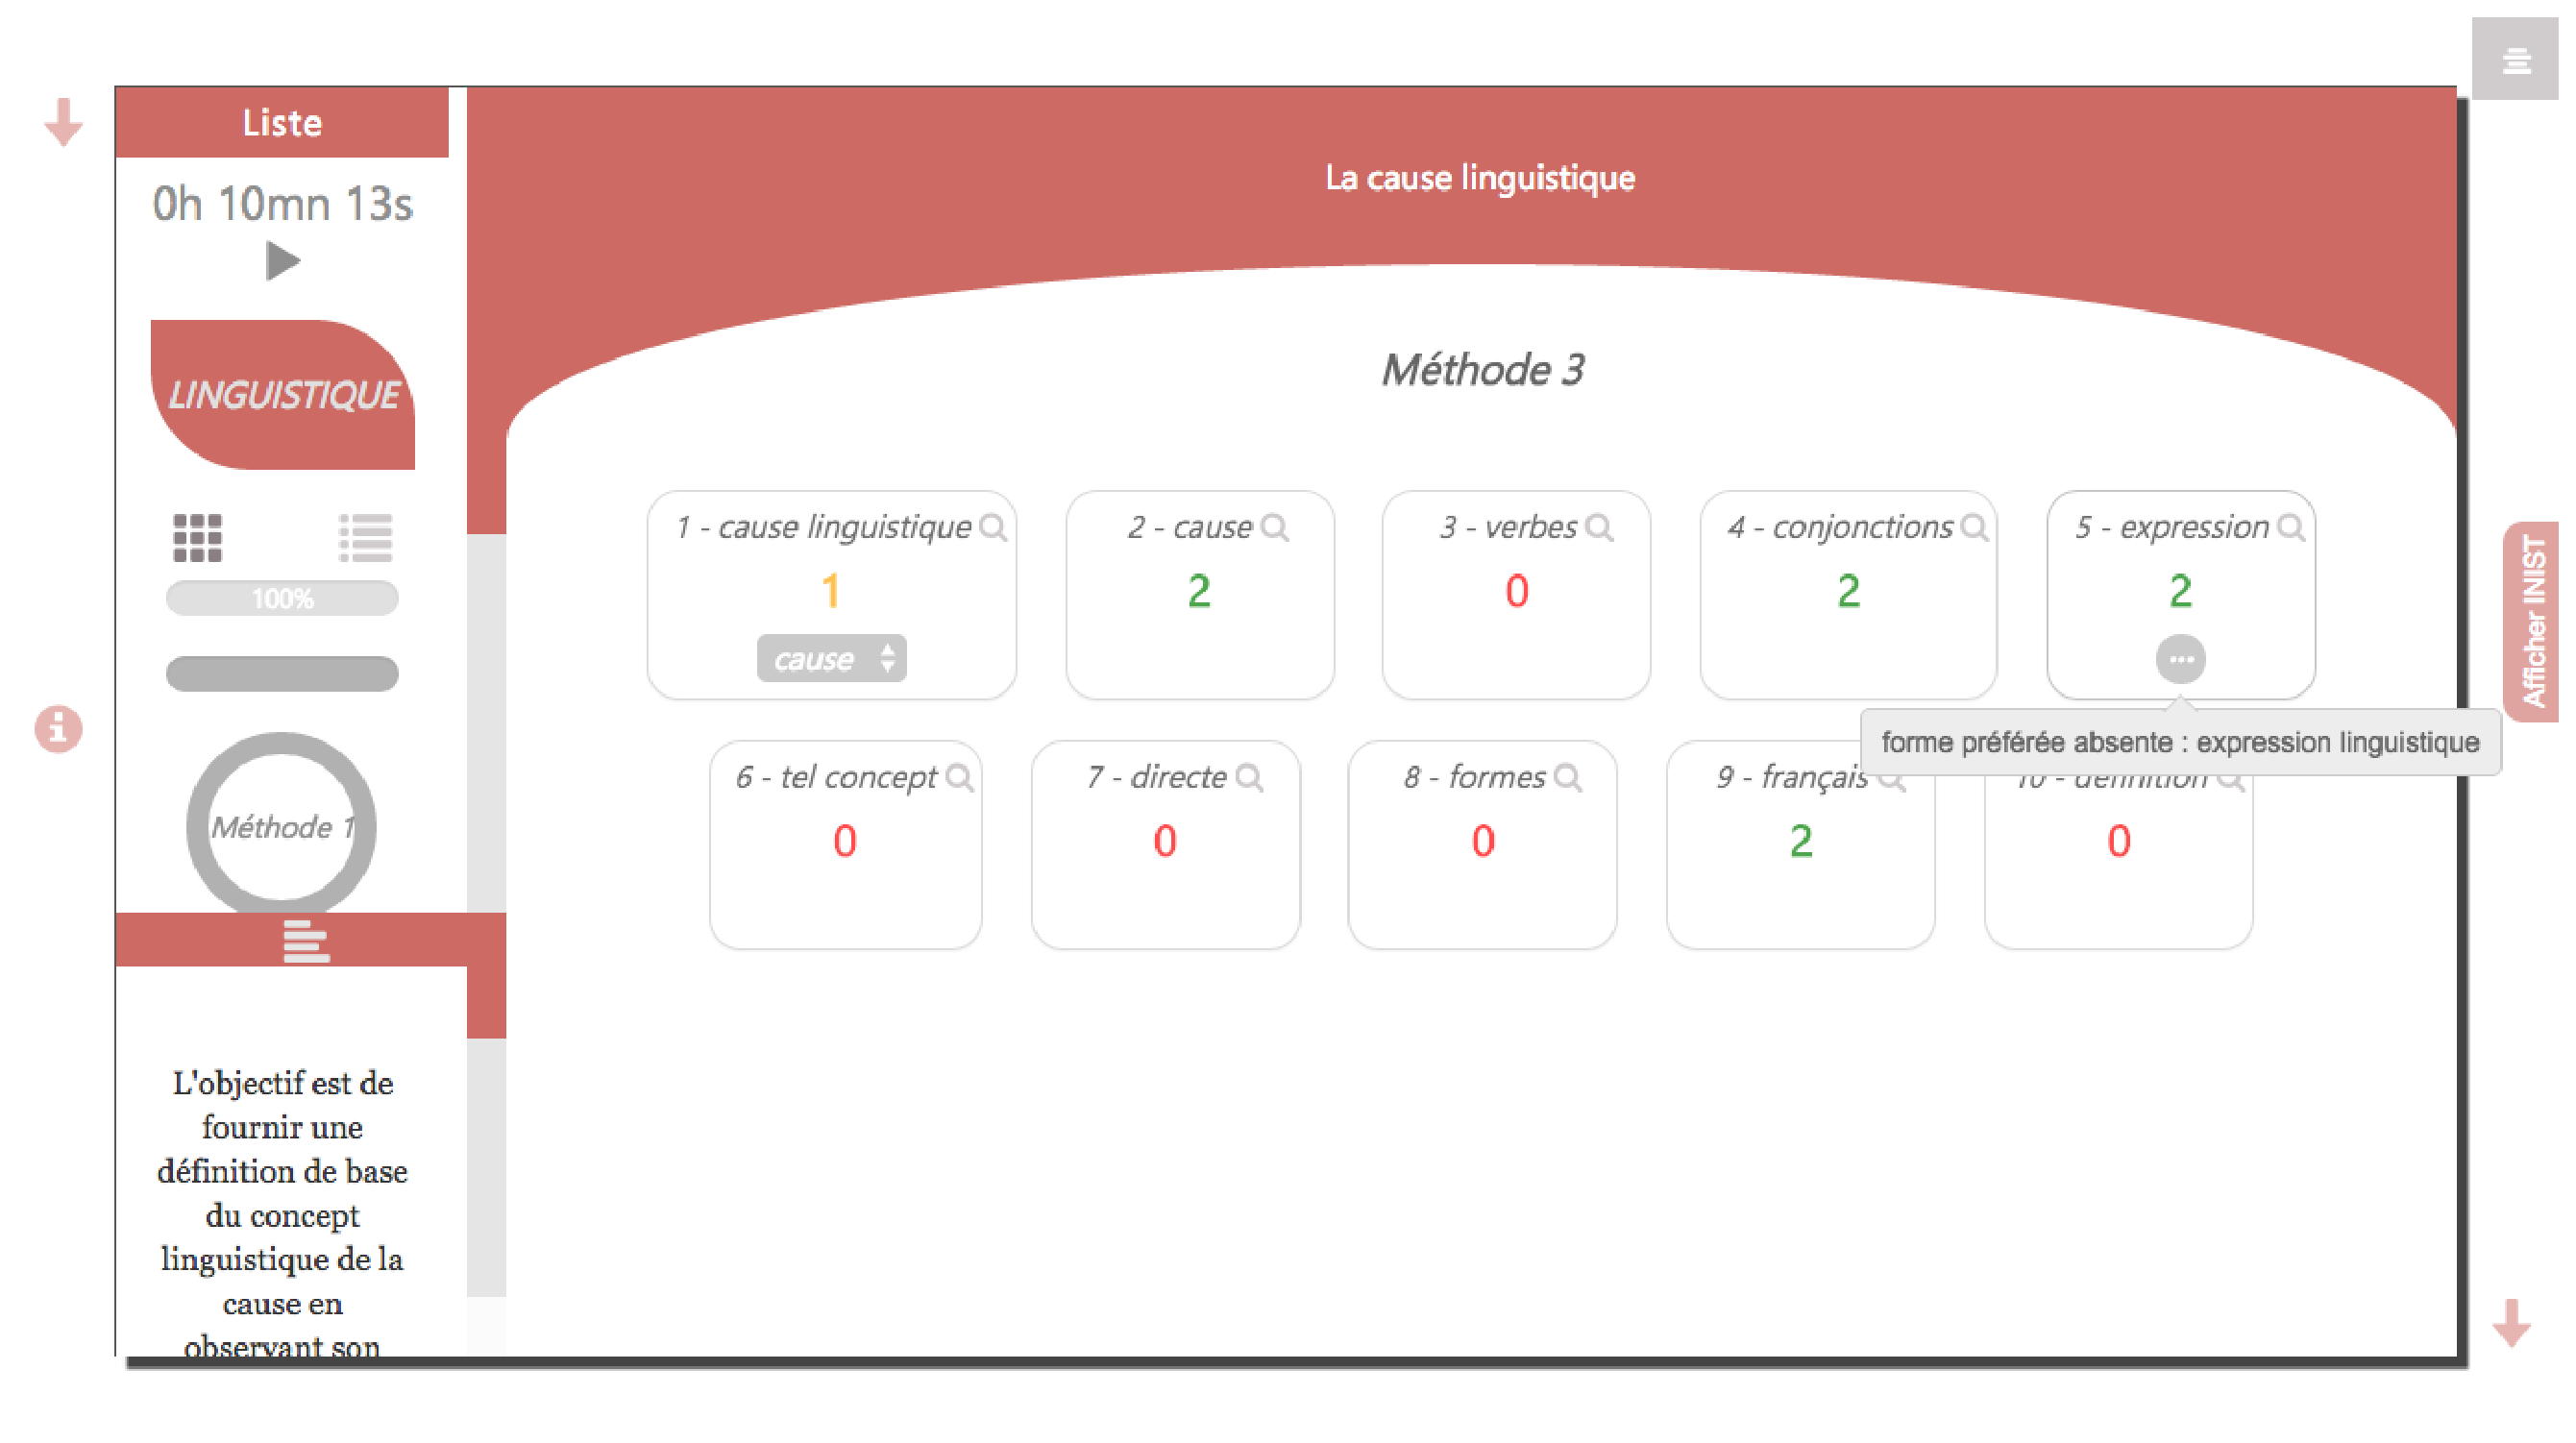
\includegraphics[width=\linewidth]{include/idefix.eps}
          \caption{Interface d'évaluation manuelle\index{evaluation manuelle@Évaluation manuelle} de l'Inist
                   \label{fig:idefix}}
        \end{figure}

      \subsubsection{Évaluation du silence}
      \label{subsubsec:main-automatic_evaluation_of_keyphrase_annotation-methodology-evaluation_protocol-silence}
        Pour évaluer le silence, l'évaluateur doit attribuer à chaque terme-clé\index{terme-cle@Terme-clé}
        de référence\index{reference@Référence} un score\index{score@Score} indiquant le degré d'importance\index{importance@Importance} de l'information
        qu'il véhicule et qui n'est pas capturée par les termes-clés\index{terme-cle@Terme-clé} fournis par
        une méthode\index{methode@Méthode} d'indexation par termes-clés\index{terme-cle@Terme-clé}. Sur une échelle de 0 à 2, ce
        score\index{score@Score} permet d'indiquer s'il n'y pas de perte d'information (0), si
        l'information perdue est capitale (2) ou si elle est secondaire (1).
        Lorsqu'un terme-clé\index{terme-cle@Terme-clé} de référence\index{reference@Référence} obtient un score\index{score@Score} de 0, cela signifie
        soit qu'il fait partie des termes-clés\index{terme-cle@Terme-clé} fournis par la méthode\index{methode@Méthode}
        d'indexation par termes-clés\index{terme-cle@Terme-clé}, soit que l'indexeur juge qu'il ne devrait
        pas être un terme-clé\index{terme-cle@Terme-clé} de référence\index{reference@Référence}, c'est-à-dire une erreur parmi les
        termes-clés\index{terme-cle@Terme-clé} de référence\index{reference@Référence}.

        Une perte d'information est jugée secondaire (score\index{score@Score} de 1) dans deux
        cas de figure~:
        \begin{itemize}
          \item{terme-clé\index{terme-cle@Terme-clé} de référence\index{reference@Référence} secondaire~: le terme-clé\index{terme-cle@Terme-clé} de référence\index{reference@Référence}
                n'apporte pas l'information la plus importante~;}
          \item{terme-clé\index{terme-cle@Terme-clé} de référence\index{reference@Référence} générique~: le terme-clé\index{terme-cle@Terme-clé} de référence\index{reference@Référence}
                n'est pas suffisamment spécifique au contenu du document\index{document@Document}, il a
                un usage classificatoire.}
        \end{itemize}
        Afin de minimiser les pertes d'informations dues à des termes-clés\index{terme-cle@Terme-clé} de
        référence\index{reference@Référence} qui ne sont pas présents dans le document\index{document@Document}, les évaluateurs
        leur attribuent un score\index{score@Score} de 1.

    \subsection{Évaluation manuelle\index{evaluation manuelle@Évaluation manuelle} des méthodes\index{methode@Méthode} proposées}
    \label{subsec:main-domain_specific_keyphrase_annotation-manual_evaluation-analysis}
      Dans cette section, nous analysons l'évaluation manuelle\index{evaluation manuelle@Évaluation manuelle} de TopicRank\index{topicrank@TopicRank},
      TopicCoRank\index{topiccorank@TopicCoRank}, d'une méthode\index{methode@Méthode} de référence\index{reference@Référence} non supervisée, \textsc{Tf-Idf\index{tf-idf@TF-IDF}},
      et d'une méthode\index{methode@Méthode} de référence\index{reference@Référence} supervisée, \textsc{Kea}\footnote{La raison
      pour laquelle les évaluations
      manuelles sont réalisées sur \textsc{Kea} et non pas \textsc{Kea++} est
      temporelle. L'évaluation manuelle\index{evaluation manuelle@Évaluation manuelle} étant coûteuse, nous n'avons pas pu
      la réitérer avec \textsc{Kea++}.}. L'évaluation est
      effectuée par un indexeur professionnel, sur la collection de linguistique
      Termith.

      Dans un premier temps, nous analysons l'évaluation manuelle\index{evaluation manuelle@Évaluation manuelle} de TopicRank\index{topicrank@TopicRank}
      et la comparons à celle de \textsc{Tf-Idf\index{tf-idf@TF-IDF}}, puis, dans un second temps,
      nous analysons l'évaluation manuelle\index{evaluation manuelle@Évaluation manuelle} de TopicCoRank\index{topiccorank@TopicCoRank} et la comparons à
      celle de \textsc{Kea}. Tous les termes-clés\index{terme-cle@Terme-clé} sont obtenus à partir des
      documents\index{document@Document} prétraités, comme nous l'avons présenté dans la
      section~\ref{sec:main-data_description-preprocessing}
      (page~\pageref{sec:main-data_description-preprocessing}). Les candidats
      sont sélectionnés à l'aide du patron grammatical \texttt{/(N|A)+/}.

      \subsubsection{Évaluation de TopicRank\index{topicrank@TopicRank}}
      \label{subsubsec:main-domain_specific_keyphrase_annotation-manual_evaluation-analysis-topicrank}
        Le
        tableau\index{tableau@Tableau}~\ref{tab:main-automatic_evaluation_of_keyphrase_annotation-results-topicrank-pertinence_score_ratio}
        montre les scores\index{score@Score} de pertinence moyens de TopicRank\index{topicrank@TopicRank} et \textsc{Tf-Idf\index{tf-idf@TF-IDF}}. Pour le score\index{score@Score}
        de 1, qui indique qu'un terme-clé\index{terme-cle@Terme-clé} est un forme variante, nous
        distinguons le cas où la variante est redondante\index{redondant@Redondant} du cas où elle ne l'est
        pas. Nous observons que TopicRank\index{topicrank@TopicRank} est meilleur\index{meilleur@Meilleur} que
        \textsc{Tf-Idf\index{tf-idf@TF-IDF}}. TopicRank\index{topicrank@TopicRank} fournit plus de termes-clés\index{terme-cle@Terme-clé} pertinents que
        \textsc{Tf-Idf\index{tf-idf@TF-IDF}}, mais fait aussi plus d'erreurs. Les termes-clés\index{terme-cle@Terme-clé} ayant
        un score\index{score@Score} de 1 donnent un explication intéressante à cette
        contradiction~: \textsc{Tf-Idf\index{tf-idf@TF-IDF}} à une forte tendance à extraire des
        termes-clés\index{terme-cle@Terme-clé} redondants\index{redondant@Redondant}, c'est-à-dire des termes-clés\index{terme-cle@Terme-clé} variantes de
        termes-clés\index{terme-cle@Terme-clé} déjà extraits, alors que TopicRank\index{topicrank@TopicRank} remplit son
        objectif de ne pas extraire de termes-clés\index{terme-cle@Terme-clé} redondants\index{redondant@Redondant}, avec seulement
        0,9~\% de redondance.
        \begin{table}[h!]
          \centering
          \begin{tabular}{l|c|c|c|c}
            \toprule
            \multirow{2}{*}{\textbf{Méthode}} & \multirow{2}{*}{\textbf{0}} & \multicolumn{2}{c|}{\textbf{1}} & \multirow{2}{*}{\textbf{2}}\\
            \cline{3-4}
            & & \multicolumn{1}{p{.175\linewidth}|}{\centering{}redondant} & \multicolumn{1}{p{.175\linewidth}|}{\centering{}non redondant} &\\
            \hline
            \textsc{Tf-Idf} & \textbf{53,8~\%} & 6,8~\% & 4,2~\% & 35,3~\%\\
            TopicRank & 56,3~\% & \textbf{0,9~\%} & \textbf{5,7~\%} & \textbf{37,1~\%}\\
            \bottomrule
          \end{tabular}
          \caption{Taux de termes-clés avec un score de 0, de 1 ou de 2 pour
                   l'évaluation de la pertinence de \textsc{Tf-Idf} et de
                   TopicRank
                   \label{tab:main-automatic_evaluation_of_keyphrase_annotation-results-topicrank-pertinence_score_ratio}}
        \end{table}

        Les résultats\index{resultat@Résultat} présentés dans le
        tableau\index{tableau@Tableau}~\ref{tab:main-automatic_evaluation_of_keyphrase_annotation-results-topicrank-pertinence_score_ratio}
        sont contraires à ceux de l'évaluation automatique, puisque c'est ici
        TopicRank\index{topicrank@TopicRank} qui est meilleur\index{meilleur@Meilleur} que \textsc{Tf-Idf\index{tf-idf@TF-IDF}} sur les documents\index{document@Document} de
        linguistique. Afin de mieux observer la différence entre l'évaluation
        manuelle et l'évaluation automatique, nous calculons la précision (P),
        le rappel (R) et la f1-mesure (F) résultantes de l'évaluation
        manuelle et les comparons aux résultats\index{resultat@Résultat} automatiques que nous avons
        montré dans le tableau\index{tableau@Tableau}~\ref{tab:resultats_inist}
        (page~\pageref{tab:resultats_inist}). Pour calculer ces performances\index{performance@Performance},
        les termes-clés\index{terme-cle@Terme-clé} ayant un score\index{score@Score} de 2 sont considérés corrects, de même
        que ceux ayant un score\index{score@Score} de 1 non redondants\index{redondant@Redondant}. Les résultats\index{resultat@Résultat} de
        l'évaluation manuelle\index{evaluation manuelle@Évaluation manuelle} comparés à ceux de l'évaluation automatique sont
        présentés dans le
        tableau\index{tableau@Tableau}~\ref{tab:main-automatic_evaluation_of_keyphrase_annotation-results-topicrank-prf}.
        
        La difficulté d'évaluer automatiquement la tâche d'indexation par
        termes-clés\index{terme-cle@Terme-clé} se confir\-me. Avec l'évaluation manuelle\index{evaluation manuelle@Évaluation manuelle}, les conclusions ne
        sont pas les mêmes, puisque de manière automatique TopicRank\index{topicrank@TopicRank} est moins
        performant que \textsc{Tf-Idf\index{tf-idf@TF-IDF}} alors qu'il est plus performant selon
        l'évaluation manuelle\index{evaluation manuelle@Évaluation manuelle}. Nous observons aussi un écart conséquent entre
        les performances\index{performance@Performance} évaluées manuellement et celles évaluées
        automatiquement. Le gain d'environ 20 points atteste le pessimisme de
        l'évaluation automatique.
        \begin{table}[h!]
          \centering
          \begin{tabular}{l|c@{~~~~~~}cc|c@{~~~~~~~~}cc}
            \toprule
            \multirow{2}{*}{\textbf{Méthode}} & \multicolumn{3}{c|}{\textbf{Évaluation manuelle}} & \multicolumn{3}{c}{\textbf{Évaluation automatique}}\\
            \cline{2-7}
            & P & R & F & P & R & F\\
            \hline
            \textsc{Tf-Idf} & 39,5 & 29,7 & 33,5 & \textbf{13,0} & \textbf{15,4} & \textbf{13,9}\\
            TopicRank & \textbf{42,8} & \textbf{32,2} & \textbf{36,2} & 11,2 & 13,1 & 11,9\\
            \bottomrule
          \end{tabular}
          \caption[
            Performances de \textsc{Tf-Idf} et de TopicRank en termes de
            précision, de rappel et de f1-mesure
          ]{
            Performances de \textsc{Tf-Idf} et de TopicRank en termes de
            précision (P), de rappel (R) et de f1-mesure (F)
            \label{tab:main-automatic_evaluation_of_keyphrase_annotation-results-topicrank-prf}}
        \end{table}
      
        ~\\Enfin, le
        tableau\index{tableau@Tableau}~\ref{tab:main-automatic_evaluation_of_keyphrase_annotation-results-topicrank-silence_score_ratio}
        montre les scores\index{score@Score} de silence attribués en moyenne par méthode\index{methode@Méthode}. D'après
        la description donnée pour chacun des scores\index{score@Score}, la méthode\index{methode@Méthode} qui capture le
        plus d'information est celle qui maximise le nombre\index{nombre@Nombre} de termes-clés\index{terme-cle@Terme-clé} de
        référence\index{reference@Référence} ayant un score\index{score@Score} de silence 0 et qui minimise ceux ayant un
        score\index{score@Score} de 1 et de 2. Nous observons donc que TopicRank\index{topicrank@TopicRank} couvre mieux le
        contenu principal des documents\index{document@Document} que \textsc{Tf-Idf\index{tf-idf@TF-IDF}}. Parce que TopicRank\index{topicrank@TopicRank}
        groupe les termes-clés\index{terme-cle@Terme-clé} candidats en sujets\index{sujet@Sujet} et n'extrait qu'un seul
        terme-clé\index{terme-cle@Terme-clé} par sujet\index{sujet@Sujet}, il y a moins de redondance parmi les termes-clés\index{terme-cle@Terme-clé}
        qu'il extrait (voir le
        tableau\index{tableau@Tableau}~\ref{tab:main-automatic_evaluation_of_keyphrase_annotation-results-topicrank-pertinence_score_ratio})
        et le nombre\index{nombre@Nombre} de sujets\index{sujet@Sujet} couverts est donc meilleur\index{meilleur@Meilleur}.
        \begin{table}[h!]
          \centering
          \begin{tabular}{l|c|c|c}
            \toprule
            \textbf{Méthode} & \textbf{0} & \textbf{1} & \textbf{2}\\
            \hline
            \textsc{Tf-Idf} & 31,4~\% & 48,5~\% & 20,1~\%\\
            TopicRank & \textbf{35,0~\%} & \textbf{48,3~\%} & \textbf{16,8~\%}\\
            \bottomrule
          \end{tabular}
          \caption{Taux de termes-clés de référence avec un score de 0, de 1 ou
                   de 2 pour l'évaluation du silence de \textsc{Tf-Idf} et de
                   TopicRank
                   \label{tab:main-automatic_evaluation_of_keyphrase_annotation-results-topicrank-silence_score_ratio}}
        \end{table}

      \subsubsection{Évaluation de TopicCoRank\index{topiccorank@TopicCoRank}}
      \label{subsubsec:main-domain_specific_keyphrase_annotation-manual_evaluation-analysis-topiccorank}
        Les résultats\index{resultat@Résultat} que nous montrons dans cette section sont obtenus avec
        seulement 25~\% de l'ensemble\index{ensemble@Ensemble} de test de la collection linguistique
        Termith\footnote{En raison de cette incomplétude de l'évaluation
        manuelle, nous ne comparons pas l'évaluation manuelle\index{evaluation manuelle@Évaluation manuelle} à l'évaluation
        automatique comme nous l'avons fait pour TopicRank\index{topicrank@TopicRank} et \textsc{Tf-Idf\index{tf-idf@TF-IDF}}.}.
        Les différentes revues qui composent la collection sont
        réparties de manière homogène dans ces 25~\%.

        Le
        tableau\index{tableau@Tableau}~\ref{tab:main-domain_specific_keyphrase_annotation-manual_evaluation-analysis-topiccorank-pertinence_score_ratio}
        montre les scores\index{score@Score} de pertinence moyens de TopicCoRank\index{topiccorank@TopicCoRank} et \textsc{Kea}.
        Nous observons que TopicCoRank\index{topiccorank@TopicCoRank} est meilleur\index{meilleur@Meilleur} que
        \textsc{Kea}. TopicCoRank\index{topiccorank@TopicCoRank} fournit plus de termes-clés\index{terme-cle@Terme-clé} pertinents que
        \textsc{Kea}, mais fait aussi plus d'erreurs. À l'instar de TopicRank\index{topicrank@TopicRank},
        TopicCoRank\index{topiccorank@TopicCoRank} est moins redondant\index{redondant@Redondant} que la méthode\index{methode@Méthode} de référence\index{reference@Référence}. Il est tout
        de même plus redondant\index{redondant@Redondant} que TopicRank\index{topicrank@TopicRank}. Cela est du au fait qu'il peut assigner un terme-clé\index{terme-cle@Terme-clé} et
        extraire une variante pouvant être jugée importante, car plus
        spécifique, ou redondante\index{redondant@Redondant}.
        \begin{table}[h!]
          \centering
          \begin{tabular}{l|c|c|c|c}
            \toprule
            \multirow{2}{*}{\textbf{Méthode}} & \multirow{2}{*}{\textbf{0}} & \multicolumn{2}{c|}{\textbf{1}} & \multirow{2}{*}{\textbf{2}}\\
            \cline{3-4}
            & & \multicolumn{1}{p{.175\linewidth}|}{\centering{}redondant} & \multicolumn{1}{p{.175\linewidth}|}{\centering{}non redondant} &\\
            \hline
            \textsc{Kea} & \textbf{45,2~\%} & 10,2~\% & \textbf{8,0~\%} & 36,6~\%\\
            TopicCoRank & 49,8~\% & \textbf{4,4~\%} & 6,2~\% & \textbf{39,6~\%}\\
            \bottomrule
          \end{tabular}
          \caption{Taux de termes-clés avec un score de 0, de 1 ou de 2 pour
                   l'évaluation de la pertinence de \textsc{Kea} et de
                   TopicCoRank
                   \label{tab:main-domain_specific_keyphrase_annotation-manual_evaluation-analysis-topiccorank-pertinence_score_ratio}}
        \end{table}

        Comparé à TopicRank\index{topicrank@TopicRank}, TopicCoRank\index{topiccorank@TopicCoRank} est effectivement plus performant. Il
        trouve plus de termes-clés\index{terme-cle@Terme-clé} corrects et fait moins d'erreurs. Cependant,
        comme nous
        l'avons dit ci-dessus, il est plus redondant\index{redondant@Redondant}. Comparée à
        \textsc{Tf-Idf\index{tf-idf@TF-IDF}} et \textsc{Kea}, cette redondance est tout de même plus
        faible.

%        \TODO{\dots}
%        \begin{table}[h!]
%          \centering
%          \begin{tabular}{l|c@{~~~~~~}cc|c@{~~~~~~~~}cc}
%            \toprule
%            \multirow{2}{*}{\textbf{Méthode\index{methode@Méthode}}} & \multicolumn{3}{c|}{\textbf{Évaluation manuelle\index{evaluation manuelle@Évaluation manuelle}}} & \multicolumn{3}{c}{\textbf{Évaluation automatique}}\\
%            \cline{2-7}
%            & P & R & F & P & R & F\\
%            \hline
%            \textsc{Kea} & 44,6 & 32,5 & 37,1 & 13,8 & 16,3 & 14,7\\
%            TopicCoRank\index{topiccorank@TopicCoRank} & \textbf{45,8} & \textbf{34.1} & \textbf{39.6} & \textbf{19,0} & \textbf{22,0} & \textbf{20,1}\\
%            \bottomrule
%          \end{tabular}
%          \caption[
%            Performances\index{performance@Performance} de \textsc{Kea} et de TopicCoRank\index{topiccorank@TopicCoRank} en termes de
%            précision, de rappel et de f-mesure
%          ]{
%            Performances\index{performance@Performance} de \textsc{Kea} et de TopicCoRank\index{topiccorank@TopicCoRank} en termes de
%            précision (P), de rappel (R) et de f-mesure (F)
%            \label{tab:main-domain_specific_keyphrase_annotation-manual_evaluation-analysis-topiccorank-prf}}
%        \end{table}
      
        ~\\Enfin, le
        tableau\index{tableau@Tableau}~\ref{tab:main-domain_specific_keyphrase_annotation-manual_evaluation-analysis-topiccorank-silence_score_ratio}
        montre les scores\index{score@Score} de silence attribués en moyenne par méthode\index{methode@Méthode}. Les
        conclusions qu'ils induisent ne sont pas en faveur de
        TopicCoRank\index{topiccorank@TopicCoRank}. En effet, même s'il ne capture pas autant de termes-clés\index{terme-cle@Terme-clé}
        que TopicCoRank\index{topiccorank@TopicCoRank}, \textsc{Kea} capture ceux qui sont sémantiquement les
        plus indispensables. Bien que les deux méthodes\index{methode@Méthode} sont supervisées,
        \textsc{Kea} est la seule des deux à apprendre à détecter les
        termes-clés\index{terme-cle@Terme-clé} à partir des traits des termes-clés\index{terme-cle@Terme-clé} du domaine\index{domaine@Domaine}. Si
        l'ordonnancement conjoint\index{conjoint@Conjoint} à base de graphe\index{graphe@Graphe} est plus efficace pour
        identifier les termes-clés\index{terme-cle@Terme-clé}, l'apprentissage permet une meilleure\index{meilleur@Meilleur}
        précision quant à l'identification de ceux les plus indispensables.
        \begin{table}[h!]
          \centering
          \begin{tabular}{l|c|c|c}
            \toprule
            \textbf{Méthode} & \textbf{0} & \textbf{1} & \textbf{2}\\
            \hline
            \textsc{Kea} & \textbf{37,3~\%} & 46,0~\% & \textbf{16,7}~\%\\
            TopicCoRank & 35,9~\% & \textbf{45,3~\%} & 18,8~\%\\
            \bottomrule
          \end{tabular}
          \caption{Taux de termes-clés de référence avec un score de 0, de 1 ou
                   de 2 pour l'évaluation du silence de \textsc{Kea} et de
                   TopicCoRank
                   \label{tab:main-domain_specific_keyphrase_annotation-manual_evaluation-analysis-topiccorank-silence_score_ratio}}
        \end{table}

    \subsection{Bilan}
    \label{subsec:main-domain_specific_keyphrase_annotation-manual_evaluation-conclusion}
      Nous avons réalisé une campagne d'évaluation manuelle\index{evaluation manuelle@Évaluation manuelle} de nos travaux en
      domaine\index{domaine@Domaine} de spécialité\index{specialite@Spécialité}, avec la collection de linguistique Termith. Pour
      cette campagne, nous avons proposé un protocole d'évaluation et des
      métriques permettant de capturer deux aspects de l'indexation par
      termes-clés\index{terme-cle@Terme-clé}~: la pertinence des termes-clés\index{terme-cle@Terme-clé} extraits/assignés et leur
      silence, c'est-à-dire la quantité d'information importante qu'ils ne
      capturent pas. Contrairement au premier aspect, qui est similaire à ce
      qu'évalue un système automatique, le dernier aspect permet d'évaluer les
      termes-clés\index{terme-cle@Terme-clé} d'un point de vu sémantique, jamais considéré auparavant.

      Les résultats\index{resultat@Résultat} montrent que, contrairement à ce que montrait l'évaluation
      automatique, TopicRank\index{topicrank@TopicRank} effectue une indexation par termes-clés\index{terme-cle@Terme-clé} de
      meilleure\index{meilleur@Meilleur} qualité que celle de \textsc{Tf-Idf\index{tf-idf@TF-IDF}}. TopicRank\index{topicrank@TopicRank} extrait peu de
      termes-clés\index{terme-cle@Terme-clé} redondants\index{redondant@Redondant} et couvre mieux le document\index{document@Document}, en partie grâce à son
      groupement des termes-clés\index{terme-cle@Terme-clé} candidats en sujets\index{sujet@Sujet}. Entre TopicCoRank\index{topiccorank@TopicCoRank},
      TopicRank\index{topicrank@TopicRank}, \textsc{Tf-Idf\index{tf-idf@TF-IDF}} et \textsc{Kea}, c'est TopicCoRank\index{topiccorank@TopicCoRank} qui trouve
      le plus de termes-clés\index{terme-cle@Terme-clé} corrects. L'évaluation du silence montre tout de
      même que c'est \textsc{Kea} qui identifie ceux jugés les plus
      indispensables par les indexeurs professionnels. Les deux aspects
      (pertinence et silence) de l'évaluation manuelle\index{evaluation manuelle@Évaluation manuelle} et leurs conclusions
      paradoxales soulèvent une nouvelle perspective pour l'évaluation
      automatique. En effet, il serait intéressant d'ordonner par importance\index{importance@Importance} les
      termes-clés\index{terme-cle@Terme-clé} de référence\index{reference@Référence} et d'en tenir compte pour identifier les méthodes\index{methode@Méthode}
      qui capturent les termes-clés\index{terme-cle@Terme-clé} les plus indispensables.

  %-----------------------------------------------------------------------------

  \section{Conclusion}
  \label{sec:main-domain_specific_keyphrase_annotation-conclusion}
    Nous nous sommes intéressé à l'indexation automatique\index{indexation automatique@Indexation automatique} par termes-clés\index{terme-cle@Terme-clé} en
    domaines\index{domaine@Domaine} de spécialité\index{specialite@Spécialité}. Nous avons tout d'abord présenté l'indexation
    manuelle réalisée par des indexeurs professionnels dans ce contexte, nous
    avons ensuite proposé une nouvelle méthode\index{methode@Méthode} automatique se rapprochant le
    plus possible de cette indexation, puis nous avons présenté les premiers
    résultats\index{resultat@Résultat} d'une campagne d'évaluation manuelle\index{evaluation manuelle@Évaluation manuelle} que nous avons réalisé avec
    des indexeurs professionnels.

    Contrairement aux méthodes\index{methode@Méthode} d'indexation automatique\index{indexation automatique@Indexation automatique}, l'indexation manuelle
    n'est pas divisée entre extraction et assignement. L'indexation manuelle en
    domaines\index{domaine@Domaine} de spécialité\index{specialite@Spécialité} préfère l'assignement, car cela permet une
    indexation homogène des documents\index{document@Document} d'un même domaine\index{domaine@Domaine} et une conformité
    vis-à-vis du vocabulaire\index{vocabulaire@Vocabulaire} spécialisé du domaine\index{domaine@Domaine}. Elle a aussi besoin de
    l'extraction, afin de fournir des termes-clés\index{terme-cle@Terme-clé} très spécifiques au document\index{document@Document},
    ainsi que pour y identifier d'éventuels nouveaux concepts.

    Pour remédier à la fracture entre extraction et assignement en indexation
    automatique par termes-clés\index{terme-cle@Terme-clé}, nous proposons TopicCoRank\index{topiccorank@TopicCoRank}. Conçu sur la base
    de TopicRank\index{topicrank@TopicRank}, TopicCoRank\index{topiccorank@TopicCoRank} utilise les données d'entraînement pour
    représenter le domaine\index{domaine@Domaine} avec un graphe\index{graphe@Graphe} unifié à celui des sujets\index{sujet@Sujet}. Cette
    unification permet d'améliorer l'ordonnancement des sujets\index{sujet@Sujet}, en tenant compte
    de leurs relations avec le domaine\index{domaine@Domaine}, et d'assigner des termes-clés\index{terme-cle@Terme-clé}, en
    puisant dans le domaine\index{domaine@Domaine}. À notre connaissance, TopicCoRank\index{topiccorank@TopicCoRank} est la seule
    méthode\index{methode@Méthode} qui réalise conjointement extraction et assignement.

    Pour valider les deux méthodes\index{methode@Méthode} TopicRank\index{topicrank@TopicRank} et TopicCoRank\index{topiccorank@TopicCoRank}, nous avons réalisé
    une campagne d'évaluation manuelle\index{evaluation manuelle@Évaluation manuelle} en domaine\index{domaine@Domaine} de spécialité\index{specialite@Spécialité}. Le protocole
    d'évaluation que nous avons proposé permet d'évaluer chaque méthode\index{methode@Méthode} selon le
    degré de pertinence des termes-clés\index{terme-cle@Terme-clé} qu'elle propose et selon le degré
    d'information qui lui échappe. Les résultats\index{resultat@Résultat} de l'évaluation manuelle\index{evaluation manuelle@Évaluation manuelle} de
    TopicRank\index{topicrank@TopicRank} son plus encourageant que ceux de l'évaluation automatique. Ils
    montrent que TopicRank\index{topicrank@TopicRank} est en réalité plus performant que \textsc{Tf-Idf\index{tf-idf@TF-IDF}},
    en partie parce qu'il couvre mieux les sujets\index{sujet@Sujet} du document\index{document@Document} grâce à son
    groupement en sujets\index{sujet@Sujet} des termes-clés\index{terme-cle@Terme-clé} candidats.
    Ils montrent aussi que TopicCoRank\index{topiccorank@TopicCoRank} est la méthode\index{methode@Méthode} la plus performante
    comparée à TopicRank\index{topicrank@TopicRank}, \textsc{Tf-Idf\index{tf-idf@TF-IDF}} et \textsc{Kea}. Cependant, c'est
    \textsc{Kea} qui trouve les termes-clés\index{terme-cle@Terme-clé} les plus indispensables.
    Au delà de cela, cette
    campagne a montré les limites de l'évaluation automatique, qui suit un
    paradigme trop strict pour la tâche d'indexation par termes-clés\index{terme-cle@Terme-clé}. Parce que
    l'évaluation manuelle\index{evaluation manuelle@Évaluation manuelle} est trop coûteuse pour être systématiquement mise en
    \oe{}uvre, il est donc important de s'intéresser de plus près aux méthodes\index{methode@Méthode}
    d'évaluation automatique. Les ressources de notre campagne, annotées étape
    par étape, seront donc
    rendues disponibles gratuitement à toute la communauté scientifique. Cette
    disponibilité permettra d'évaluer de nouvelles méthodes\index{methode@Méthode} d'évaluation, en
    vérifiant leur corrélation avec l'évaluation manuelle\index{evaluation manuelle@Évaluation manuelle} des indexeurs
    professionnels.


  \chapter{Conclusion et perspectives}
\label{chap:main-conclusion}
  \chaptercite{
    [...] la tâche est loin d'être résolue [...]
%    [\dots] the task is far from being solved [\dots]
  }{
    \newcite{hasan2014state_of_the_art}
  }{.75\linewidth}{\hfill}

  Dans cette thèse, nous nous sommes intéressé à la tâche d'indexation par
  termes-clés\index{terme-cle@Terme-clé} en domaines\index{domaine@Domaine} de spécialité\index{specialite@Spécialité}. Étant donné un document\index{document@Document} textuel, cette
  tâche consiste à lui attribuer les unités textuelles\index{unite textuelle@Unité textuelle} qui décrivent son
  contenu. Ces unités textuelles\index{unite textuelle@Unité textuelle}, les termes-clés\index{terme-cle@Terme-clé}, permettent de le résumer, de
  le catégoriser et, surtout, de l'indexer pour la recherche d'information. Les
  termes-clés\index{terme-cle@Terme-clé} peuvent être attribués par les auteurs, des lecteurs ou des
  indexeurs professionnels, mais seuls ces derniers réalisent un travail
  impartial, homogène et conforme à une indexation de qualité en domaines\index{domaine@Domaine} de
  spécialité\index{specialite@Spécialité}. Notre objectif est de proposer une alternative automatique aux
  indexeurs professionnels pour une indexation par termes-clés\index{terme-cle@Terme-clé} de documents\index{document@Document}
  numériques en domaines\index{domaine@Domaine} de spécialité\index{specialite@Spécialité}. Tout d'abord, nous avons fait le choix
  de traiter ce problème dans sa généralité, puis nous nous sommes ensuite
  concentré sur les documents\index{document@Document} en domaines\index{domaine@Domaine} de spécialité\index{specialite@Spécialité} et sur leur indexation
  particulière effectuée par des indexeurs professionnels.

  Dans la littérature, de nombreuses méthodes\index{methode@Méthode} sont proposées pour l'indexation
  automatique par termes-clés\index{terme-cle@Terme-clé}. Elles sont réparties en deux catégories~:
  l'extraction et l'assignement de termes-clés\index{terme-cle@Terme-clé}. La première extrait les
  termes-clés\index{terme-cle@Terme-clé} depuis le contenu du document\index{document@Document}. Il s'agit de la catégorie
  d'indexation par termes-clés\index{terme-cle@Terme-clé} la plus étudiée. Elle est plus simple à mettre en
  \oe{}uvre, car elle traite les unités textuelles\index{unite textuelle@Unité textuelle} du document\index{document@Document}. Cependant, ces
  unités textuelles\index{unite textuelle@Unité textuelle} ne sont pas toujours sous une forme appropriée. La seconde
  assigne les termes-clés\index{terme-cle@Terme-clé} depuis un vocabulaire\index{vocabulaire@Vocabulaire} contrôlé représentatif du
  langage documentaire. Elle assure donc une indexation de meilleure\index{meilleur@Meilleur} qualité.
  Cependant, elle est plus difficile à mettre en \oe{}uvre, car les entrées du
  vocabulaire\index{vocabulaire@Vocabulaire} contrôlé ne sont pas nécessairement présentes dans le document\index{document@Document}.
  Par ailleurs, elle n'est pas capable d'identifier des termes-clés\index{terme-cle@Terme-clé} très
  spécifiques au document\index{document@Document} s'ils ne sont pas dans le vocabulaire\index{vocabulaire@Vocabulaire} contrôlé, ni
  même des nouveaux concepts. Pour traiter le problème d'indexation par
  termes-clés\index{terme-cle@Terme-clé} dans sa généralité, nous avons travaillé sur l'extraction de
  termes-clés\index{terme-cle@Terme-clé}. Pour l'indexation en domaines\index{domaine@Domaine} de spécialité\index{specialite@Spécialité}, nous avons proposé
  une extension de ce travail afin d'y intégrer la capacité à réaliser
  l'assignement.

  \section{Contributions}
  \label{sec:main-conclusion-contributions}
    Nos travaux ont fait l'objet de trois contributions~: deux contributions
    pour l'extraction de termes-clés\index{terme-cle@Terme-clé} et une contribution pour l'indexation par
    termes-clés\index{terme-cle@Terme-clé} en domaines\index{domaine@Domaine} de spécialité\index{specialite@Spécialité}. Nous avons aussi proposé un
    protocole d'évaluation pour une campagne d'évaluation manuelle\index{evaluation manuelle@Évaluation manuelle} de nos
    travaux.

    Notre première contribution à l'extraction de termes-clés\index{terme-cle@Terme-clé} concerne l'étape
    préliminaire de sélection\index{selection@Sélection} des termes-clés\index{terme-cle@Terme-clé} candidats. Elle consiste à
    identifier les unités textuelles\index{unite textuelle@Unité textuelle} du document\index{document@Document} susceptibles d'être des
    termes-clés\index{terme-cle@Terme-clé}. Dans la littérature, cette étape est très souvent réalisée à
    l'aide de règles simples qui ont tendance à sélectionner beaucoup de
    candidats. Or, nous émettons l'hypothèse que l'indexation gagne en
    efficacité lorsque la sélection\index{selection@Sélection} des candidats fournie un ensemble\index{ensemble@Ensemble} de petite
    taille contenant le plus possible de termes-clés\index{terme-cle@Terme-clé} corrects.
    %
    En nous fondant sur une analyse des propriétés linguistiques des termes-clés\index{terme-cle@Terme-clé}
    de référence\index{reference@Référence}, nous avons d'abord proposé une méthode\index{methode@Méthode} qui limite le nombre\index{nombre@Nombre} de
    candidats sélectionnés en ciblant les séquences de noms\index{nom@Nom} modifiés, ou non,
    par un adjectif\index{adjectif@Adjectif} utile (non superflu). Un adjectif\index{adjectif@Adjectif} utile se distingue par sa
    catégorie, relationnel\index{relationnel@Relationnel} ou composé complexe, et son usage fréquent dans le
    document\index{document@Document}~; un adjectif\index{adjectif@Adjectif} superflu est un adjectif\index{adjectif@Adjectif} qualificatif qui modifie
    n'importe quel nom\index{nom@Nom}.
    %
    Nous avons ensuite vérifié notre hypothèse en évaluant la qualité de
    l'ensemble\index{ensemble@Ensemble} de candidats sélectionnés par notre méthode\index{methode@Méthode}, ainsi que son impact
    sur deux méthodes\index{methode@Méthode} d'extraction de termes-clés\index{terme-cle@Terme-clé}~:
    \textsc{Tf-Idf\index{tf-idf@TF-IDF}}~\cite{salton1975tfidf} et \textsc{Kea}~\cite{witten1999kea}.
    Les résultats\index{resultat@Résultat} ont montré que notre méthode\index{methode@Méthode} est capable de réduire le nombre\index{nombre@Nombre}
    de candidats sélectionnés sans éliminer un nombre\index{nombre@Nombre} significatif de
    termes-clés\index{terme-cle@Terme-clé} corrects. Ils montrent aussi qu'elle a une meilleure\index{meilleur@Meilleur} influence
    sur la performance\index{performance@Performance} des méthodes\index{methode@Méthode} d'extractions employées.

    Notre seconde contribution à l'extraction de termes-clés\index{terme-cle@Terme-clé} s'intéresse aux
    méthodes\index{methode@Méthode} qui ordonnent les termes-clés\index{terme-cle@Terme-clé} candidats par importance\index{importance@Importance}, puis
    extraient les $k$ plus importants en tant que termes-clés\index{terme-cle@Terme-clé}. Selon nous, ce ne
    sont pas les termes-clés\index{terme-cle@Terme-clé} candidats qui doivent être ordonnés par importance\index{importance@Importance},
    mais ce qu'ils représentent~: leur sujet\index{sujet@Sujet}. De plus, si plusieurs unités
    textuelles représentent le même sujet\index{sujet@Sujet}, alors elles doivent être considérées
    comme une entité unique. Nous avons donc proposé, TopicRank\index{topicrank@TopicRank}, une méthode\index{methode@Méthode} à
    base de graphe\index{graphe@Graphe} qui commence par grouper les termes-clés\index{terme-cle@Terme-clé} candidats en sujets\index{sujet@Sujet},
    représente le document\index{document@Document} avec un graphe\index{graphe@Graphe} des sujets\index{sujet@Sujet}, ordonne ces sujets\index{sujet@Sujet} à
    l'aide d'un algorithme de marche aléatoire dans le graphe\index{graphe@Graphe}, puis extrait un,
    et un seul, terme-clé\index{terme-cle@Terme-clé} candidat pour chacun des $k$ meilleurs\index{meilleur@Meilleur} sujets\index{sujet@Sujet}. Nos
    expériences ont montré une amélioration de l'extraction de termes-clés\index{terme-cle@Terme-clé}
    avec TopicRank\index{topicrank@TopicRank}, comparée à celle réalisée avec les autres méthodes\index{methode@Méthode} à base de
    graphe\index{graphe@Graphe}, TextRank~\cite{mihalcea2004textrank} et
    SingleRank~\cite{wan2008expandrank}. Au
    travers d'évaluations manuelles\index{evaluation manuelle@Évaluation manuelle}, nous avons aussi pu montrer que TopicRank\index{topicrank@TopicRank}
    extrait des termes-clés\index{terme-cle@Terme-clé} non redondants\index{redondant@Redondant}, lui permettant de mieux couvrir les
    sujets\index{sujet@Sujet} du document\index{document@Document} que les autres méthodes\index{methode@Méthode}.

    Notre troisième contribution s'intéresse à l'indexation par termes-clés\index{terme-cle@Terme-clé} en
    domaines\index{domaine@Domaine} de spécialité\index{specialite@Spécialité} telle qu'elle est effectuée par un indexeur
    professionnel. Ces indexeurs mêlent extraction et assignement, avec une
    préférence pour l'assignement. L'assignement permet d'obtenir une indexation
    homogène de tous les documents\index{document@Document} d'un même domaine\index{domaine@Domaine}, une indexation conforme au
    vocabulaire\index{vocabulaire@Vocabulaire} de ce domaine\index{domaine@Domaine} et une généralisation du contenu de chaque
    document\index{document@Document} afin de le situer dans son domaine\index{domaine@Domaine}. L'extraction, quant à elle,
    permet d'améliorer l'exhaustivité de l'indexation en ajoutant des
    termes-clés\index{terme-cle@Terme-clé} très spécifiques au document\index{document@Document}, voir même de nouveaux concepts.
    Nous faisons donc l'hypothèse qu'extraction et assignement doivent être
    réalisés conjointement grâce à une contextualisation du contenu du
    document\index{document@Document} dans son domaine\index{domaine@Domaine}. Cette contextualisation doit (1) permettre de
    déterminer l'importance\index{importance@Importance} des sujets\index{sujet@Sujet} en tenant aussi compte de la place qu'ils
    occupent dans le domaine\index{domaine@Domaine} et (2) permettre l'assignement en déterminant les
    termes-clés\index{terme-cle@Terme-clé} du domaines\index{domaine@Domaine} importants vis-à-vis du document\index{document@Document}.
    %
    Pour cela, nous avons étendu notre seconde contribution en ajoutant un
    graphe\index{graphe@Graphe} du domaine\index{domaine@Domaine}, représenté par son vocabulaire\index{vocabulaire@Vocabulaire} contrôlé (ses
    termes-clés\index{terme-cle@Terme-clé}). Notre nouvelle méthode\index{methode@Méthode}, TopicCoRank\index{topiccorank@TopicCoRank}, représente le domaine\index{domaine@Domaine} du
    document\index{document@Document} avec un graphe\index{graphe@Graphe} des termes-clés\index{terme-cle@Terme-clé} de référence\index{reference@Référence} attribués à des
    documents\index{document@Document} du même domaine\index{domaine@Domaine}, le connecte au graphe\index{graphe@Graphe} de sujets\index{sujet@Sujet} et ordonne
    conjointement sujets\index{sujet@Sujet} et termes-clés\index{terme-cle@Terme-clé} du domaine\index{domaine@Domaine}. Les termes-clés\index{terme-cle@Terme-clé} obtenus à
    partir du graphe\index{graphe@Graphe} de sujets\index{sujet@Sujet} sont extraits et les termes-clés\index{terme-cle@Terme-clé} obtenus à partir
    du graphe\index{graphe@Graphe} du domaine\index{domaine@Domaine} sont assignés. En domaine\index{domaine@Domaine} de spécialité\index{specialite@Spécialité}, TopicCoRank\index{topiccorank@TopicCoRank}
    obtient des résultats\index{resultat@Résultat} supérieurs à l'état de l'art. À notre connaissance, il
    s'agit de la première méthode\index{methode@Méthode} capable de réaliser simultanément
    extraction et assignement.

    Enfin, nous avons participé à la mise en place d'une campagne d'évaluation
    manuelle en domaines\index{domaine@Domaine} de spécialité\index{specialite@Spécialité}. Nous avons proposé, en collaboration
    avec les indexeurs professionnels de l'Inist, un protocole permettant
    d'évaluer deux aspects de l'indexation~: la pertinence (validité) et le
    silence (perte d'information). Le premier aspect est celui qui est aussi
    évalué par l'évaluation automatique. Les résultats\index{resultat@Résultat} obtenus lors de la
    campagne ont tout de même montré l'importance\index{importance@Importance} de réaliser une évaluation
    manuelle. Celle-ci est moins pessimiste (plus juste) et nous observons un
    gain de plus de 20 points de f1-mesure par rapport à l'évaluation
    automatique. Le second aspect est nouveau pour
    l'évaluation de méthodes\index{methode@Méthode} d'indexation par termes-clés\index{terme-cle@Terme-clé}. Il est purement
    sémantique et permet de déterminer si, au delà de fournir un grand nombre\index{nombre@Nombre} de
    termes-clés\index{terme-cle@Terme-clé} corrects, la méthode\index{methode@Méthode} capture les informations les plus
    importantes du document\index{document@Document}. Toutes les ressources de cette campagne
    d'évaluation seront rendues disponibles. Elles sont annotées avec
    chaque étape (indexation automatique\index{indexation automatique@Indexation automatique} par termes-clés\index{terme-cle@Terme-clé} et évaluation manuelle\index{evaluation manuelle@Évaluation manuelle})
    afin de permettre l'étude de nouvelle méthodes\index{methode@Méthode} d'évaluation automatique,
    notamment vérifier leur corrélation avec le jugement humain.

  \section{Perspectives}
  \label{sec:main-conclusion-contributions}
    Nos contributions ont montré des améliorations en matière de sélection\index{selection@Sélection} de
    termes-clés\index{terme-cle@Terme-clé}, d'extraction de termes-clés\index{terme-cle@Terme-clé} et d'indexation par termes-clés\index{terme-cle@Terme-clé} en
    domaines\index{domaine@Domaine} de spécialité\index{specialite@Spécialité}. Elles ont toutefois des limites et il reste encore
    plusieurs perspectives de travail.

    Nous identifions trois limites de notre travail s'intéressant à la sélection\index{selection@Sélection}
    des termes-clés\index{terme-cle@Terme-clé} candidats pour l'extraction de termes-clés\index{terme-cle@Terme-clé}. Premièrement,
    notre étude linguistique des termes-clés\index{terme-cle@Terme-clé} s'est limitée aux adjectifs\index{adjectif@Adjectif}
    composés complexes et aux adjectifs\index{adjectif@Adjectif} relationnels\index{relationnel@Relationnel}, alors qu'il existe
    d'autres catégories d'adjectifs\index{adjectif@Adjectif}. Les adjectifs\index{adjectif@Adjectif} relationnels\index{relationnel@Relationnel}, qui sont des
    dénominaux, ont montré leur utilité au sein des termes-clés\index{terme-cle@Terme-clé}. Nous
    envisageons donc d'étudier n'importe quel adjectif\index{adjectif@Adjectif} dénominal, en nous
    affranchissant de ses autres propriétés, ainsi que les adjectifs\index{adjectif@Adjectif} déverbaux.
    Ensuite, nous avons mis de côté les prépositions (et les déterminants) en
    français, alors qu'ils sont constitutifs d'environ $\unitfrac{1}{3}$ des
    termes-clés\index{terme-cle@Terme-clé}. L'attachement prépositionnel au nom\index{nom@Nom} est
    ambigu~\cite{colonna2002ambiguitesyntaxique} et les prépositions (et les
    déterminants) étant d'usage fréquent dans tout discours (prépositions et
    déterminants font partie des mots\index{mot@Mot} les plus fréquents du français), cette
    ambiguïté doit absolument être résolue pour éviter d'ajouter un nombre\index{nombre@Nombre}
    conséquent d'erreurs dans l'ensemble\index{ensemble@Ensemble} des termes-clés\index{terme-cle@Terme-clé} candidats.
    %
%    alors n'en
%    est-il pas de même pour les autres adjectifs\index{adjectif@Adjectif} dénominaux~? N'est-ce pas parce
%    qu'ils sont dérivé du nom\index{nom@Nom}, élément central du terme-clé\index{terme-cle@Terme-clé}, qu'ils sont si
%    utiles~? Qu'en est-il pour les autres adjectifs\index{adjectif@Adjectif} dérivés~? Ces questions sont
%    intéressantes et mérites d'être soulevées. Ensuite, nous avons mis de côté
%    les prépositions et les déterminants en français, alors qu'ils sont
%    fréquemment employés au sein de termes-clés\index{terme-cle@Terme-clé}. Ils méritent aussi d'être
%    étudiés afin de distinguer dans quels cas ils servent de frontière entre
%    deux candidats (\TODO{exemple\index{exemple@Exemple}}) et dans quels cas ils doivent être
%    sélectionnés au sein d'eux (\TODO{exemple\index{exemple@Exemple}}).
    %
%    Enfin, lors de notre analyse de
%    TopicRank\index{topicrank@TopicRank} selon les différentes méthodes\index{methode@Méthode} de sélection\index{selection@Sélection} des termes-clés\index{terme-cle@Terme-clé}
%    candidats, nous avons évoqué la possibilité que certaines méthodes\index{methode@Méthode} (comme
%    TopicRank\index{topicrank@TopicRank}) soient moins sensibles à la variation de qualité des candidats
%    que d'autres. Il serait intéressant d'étudier les méthodes\index{methode@Méthode} de sélection\index{selection@Sélection} de
%    candidats sur un plus large panel de méthodes\index{methode@Méthode}, de vérifier cette hypothèse
%    et d'identifier quels sont les facteurs en cause d'une sensibilité plus ou
%    moins forte.

    Notre travail sur TopicRank\index{topicrank@TopicRank} possède aussi quelques limitations. Tout
    d'abord, le groupement en sujets\index{sujet@Sujet} que nous avons proposé est naïf. Il ne
    tient pas compte du lien de synonymie des mots\index{mot@Mot}, ni même de leur sens dans
    leurs contextes (problème d'ambiguïté). Nous avons proposé ce groupement car
    il permet à TopicRank\index{topicrank@TopicRank} d'être applicable dans toutes les situations, sans
    nécessiter de ressources particulières. Lorsque les données mises à
    dispositions le permettent, il serait intéressant d'envisager d'autres
    méthodes\index{methode@Méthode} de groupement. Nous pourrions analyser la sémantique latente au
    sein d'une collection donnée, comme l'ont fait
    \newcite{liu2010topicalpagerank}, \newcite{ding2011binaryintegerprogramming}
    et \newcite{zhang2013wordtopicmultirank} avec
    \textsc{Lda}~\cite{blei2003lda}. Nous pourrions aussi nous appuyer sur des
    ressources lexicales, ou des méthodes\index{methode@Méthode} automatiques, pour détecter les
    candidats qui sont synonymes et les grouper. Une autre limite de notre
    travail est le choix non optimal du terme-clé\index{terme-cle@Terme-clé} candidat à extraire pour un
    sujet\index{sujet@Sujet}. Bien que la stratégie\index{strategie@Stratégie} que nous employons donne des résultats\index{resultat@Résultat}
    satisfaisants, nous avons établi que la stratégie\index{strategie@Stratégie} optimale permettrait
    d'atteindre des performances\index{performance@Performance} deux fois supérieures dans certains cas. Une
    première solution serait d'utiliser une collection d'entraînement pour
    apprendre à reconnaître le terme-clé\index{terme-cle@Terme-clé} au sein d'un sujet\index{sujet@Sujet}. Certains traits
    utilisés par les méthodes\index{methode@Méthode} supervisés pourraient servir (position de la
    première occurrence, nombre\index{nombre@Nombre} de mots\index{mot@Mot}, etc.), ainsi que de nouveaux traits
    liés à la relation qu'entretient le candidat avec les autres candidats du
    sujet\index{sujet@Sujet} (degré de similarité avec tous les autres, catégorie grammaticale des
    mots\index{mot@Mot} en communs avec les autres, etc.). Une autre solution serait
    d'appliquer des méthodes\index{methode@Méthode} de titrage automatique, telles que celle de
    \newcite{lau2011topiclabeling}. L'avantage de cette méthode\index{methode@Méthode} est de
    permettre de générer des unités textuelles\index{unite textuelle@Unité textuelle} à partir d'un sujet\index{sujet@Sujet}. Dans notre
    cas, elle permet donc de proposer des termes-clés\index{terme-cle@Terme-clé} qui n'occurrent pas
    nécessairement dans le document\index{document@Document}. Correctement paramétrée avec un vocabulaire\index{vocabulaire@Vocabulaire}
    contrôlé, une méthode\index{methode@Méthode} de titrage automatique générative peut donc être une
    alternative à TopicCoRank\index{topiccorank@TopicCoRank} pour réaliser extraction et assignement.

    TopicCoRank\index{topiccorank@TopicCoRank}, qui permet de réaliser simultanément extraction et assignement
    de ter\-mes-clés possède aussi quelques limites. Premièrement, bien que
    l'ordonnancement conjoint\index{conjoint@Conjoint} des sujets\index{sujet@Sujet} du document\index{document@Document} et des termes-clés\index{terme-cle@Terme-clé} du
    domaine\index{domaine@Domaine} améliore l'ordonnancement, nous avons observé que TopicCoRank\index{topiccorank@TopicCoRank} est
    plus performant en domaines\index{domaine@Domaine} de spécialité\index{specialite@Spécialité} lorsqu'il ne réalise que
    l'assignement. Cela signifie que les termes-clés\index{terme-cle@Terme-clé} du domaine\index{domaine@Domaine} sont
    correctement identifiés parmi tous les termes-clés\index{terme-cle@Terme-clé} de celui-ci, mais que
    leur importance\index{importance@Importance} est trop faible comparée à celle qui est attribuée aux
    sujets\index{sujet@Sujet} du document\index{document@Document}. Ce problème peut être résolu de deux manières. Il existe
    peut être un schéma de pondération des arêtes et d'unification des deux
    graphes\index{graphe@Graphe} plus performant que celui que nous proposons. Pour unifier les deux
    graphes\index{graphe@Graphe}, nous pourrions par exemple\index{exemple@Exemple} nous intéresser au contenu des documents\index{document@Document}
    de référence\index{reference@Référence}. Ainsi, un terme-clé\index{terme-cle@Terme-clé} du domaine\index{domaine@Domaine} pourrait être connecté à un
    sujet\index{sujet@Sujet} lorsqu'il est le terme-clé\index{terme-cle@Terme-clé} d'un document\index{document@Document} dans lequel le sujet\index{sujet@Sujet}
    apparaît. Une autre manière de résoudre ce problème serait aussi de faire
    varier l'influence de la recommandation interne (paramètre $\lambda$)
    différemment pour les sujets\index{sujet@Sujet} et les termes-clés\index{terme-cle@Terme-clé} de référence\index{reference@Référence}. En augmentant
    plus fortement l'impact de la recommandation issue des sujets\index{sujet@Sujet}
    (recommandation externe) avec une faible valeur pour $\lambda$,
    l'importance\index{importance@Importance} des termes-clés\index{terme-cle@Terme-clé} du domaine\index{domaine@Domaine} devrait augmenter, leur permettant
    de rivaliser avec les sujets\index{sujet@Sujet} dans le classement par importance\index{importance@Importance}. Le paramétrage de
    $\lambda$ peut aussi résoudre un autre problème de TopicCoRank\index{topiccorank@TopicCoRank}. En effet,
    nous avons aussi observé que TopicCoRank\index{topiccorank@TopicCoRank} fonctionne moins bien hors domaines\index{domaine@Domaine}
    de spécialité\index{specialite@Spécialité}, il est difficilement généralisable. Utiliser un paramètre
    $\lambda$ différent pour calculer l'importance\index{importance@Importance} des sujets\index{sujet@Sujet} et l'importance\index{importance@Importance}
    des termes-clés\index{terme-cle@Terme-clé} peut aussi résoudre ce problème. Nous pourrions le
    paramétrer empiriquement avec les données d'entraînement, mais nous
    aimerions aussi chercher à prédire sa valeur. En effet, nous avons expliqué
    que le problème de généralisation de TopicCoRank\index{topiccorank@TopicCoRank} est dû au fait que les
    données d'entraînement des collections que nous avons utilisé hors domaines\index{domaine@Domaine}
    de spécialité\index{specialite@Spécialité} ne sont pas adaptées. Il serait donc intéressant de voir si
    nous pouvons évaluer avec quel degré les données sont adaptées et de voir
    s'il existe une corrélation entre celui-ci et le paramétrage de $\lambda$.
    Enfin, les données en domaines\index{domaine@Domaine} de spécialité\index{specialite@Spécialité} que nous utilisons ne
    contiennent que des notices. Il serait intéressant de voir les différences
    de performance\index{performance@Performance} en utilisant les articles complets que représentent ces notices.

    ~\\L'ensemble\index{ensemble@Ensemble} des travaux de cette thèse permet d'améliorer l'indexation
    automatique par termes-clés\index{terme-cle@Terme-clé}. Nos travaux en extraction de termes-clés\index{terme-cle@Terme-clé} sont
    applicables dans presque tous les scénarios d'utilisation. Aucune ressource
    externe n'est nécessaire à l'exception de celles requises par les outils de
    prétraitement (segmentation et étiquetage grammatical). Ceux en
    extraction et assignement simultanés de termes-clés\index{terme-cle@Terme-clé} sont applicables en
    domaines\index{domaine@Domaine} de spécialité\index{specialite@Spécialité}, dès lors que des données d'entraînement sont
    disponibles. Dans le cadre du projet Termith, les résultats\index{resultat@Résultat} de nos travaux
    seront exploités pour faciliter la recherche d'information avec les outils
    que propose l'Inist. TopicCoRank\index{topiccorank@TopicCoRank} identifie plus de termes-clés\index{terme-cle@Terme-clé} corrects que
    les autres méthodes\index{methode@Méthode}, ce qui facilitera le travail des indexeurs
    professionnels.
    %
    Il est aussi envisagé de s'en servir pour réaliser de
    la veille terminologique, c'est-à-dire mettre à jour des bases
    terminologiques de domaines\index{domaine@Domaine} de spécialité\index{specialite@Spécialité} avec les termes-clés\index{terme-cle@Terme-clé} validés par
    un indexeur professionnel.

%    ~\\L'ensemble\index{ensemble@Ensemble} des travaux de cette thèse permet d'améliorer l'indexation par
%    termes-clés\index{terme-cle@Terme-clé} d'un point de vue linguistique et  d'un point de vue de
%    modélisation et d'analyse du document\index{document@Document} à l'aide, ou non, de son domaine\index{domaine@Domaine}.
%    L'indexation par termes-clés\index{terme-cle@Terme-clé} que nous proposons peut-être utilisée pour la
%    recherche d'information, comme dans le cadre du travail de maintient de
%    bases de données bibliographiques de l'Inist, mais aussi pour d'autres
%    applications que nous n'avons pas évoqué, telles que la veille
%    terminologique, ou encore l'amélioration de l'effort de lecture par la mise
%    en évidence des termes-clés\index{terme-cle@Terme-clé}.


  \chapter*{Publications}
\addcontentsline{toc}{chapter}{Publications}
  \section*{Publication en revue}
  \addcontentsline{toc}{section}{Publication en revue}

  TopicRank : ordonnancement de sujets pour l'extraction automatique de
  termes-clés\\\textbf{Adrien Bougouin et Florian
  Boudin}\\\cite{bougouin2014topicrank}

  ~\\\textbf{Résumé~:}
  Les termes-clés sont les mots ou les expressions polylexicales qui
  représentent le contenu principal d'un document. Ils sont utiles pour diverses
  applications telles que l'indexation automatique ou le résumé automatique,
  mais ne sont cependant pas disponibles pour la plupart des documents. La
  quantité de ces documents étant de plus en plus importante, l'extraction
  manuelle des termes-clés n'est pas envisageable et la tâche d'extraction
  automatique de termes-clés suscite alors l'intérêt des chercheurs. Dans cet
  article nous présentons \textit{Topic\-Rank}, une méthode non supervisée à
  base de graphe pour l'extraction de termes-clés. Cette méthode groupe les
  termes-clés candidats en sujets, ordonne les sujets et extrait de chacun des
  meilleurs sujets le terme-clé candidat qui le représente le mieux. Les
  expériences réalisées montrent une amélioration significative vis-à-vis de
  l'état de l'art des méthodes à base de graphe pour l'extraction non supervisée
  de termes-clés.

  ~\\Publié dans la revue Traitement Automatique des Langues (\textsc{Tal}
  55-1).

  \section*{Publication en conférence internationale avec acte}
  \addcontentsline{toc}{section}{Publication en conférence internationale avec
  acte}

  \textit{TopicRank: Graph-Based Topic Ranking for Keyphrase
  Extraction}\\\textbf{Adrien Bougouin, Florian Boudin et Béatrice
  Daille}\\\cite{bougouin2013topicrank}

  ~\\\textit{
    \textbf{Abstract:}
    Keyphrase extraction is the task of identifying single or multi-word
    expressions that represent the main topics of a document. In this paper we
    present TopicRank, a graph-based keyphrase extraction method that relies on
    a topical representation of the document. Candidate keyphrases are clustered
    into topics and used as vertices in a complete graph. A graph-based ranking
    model is applied to assign a significance score to each topic. Keyphrases
    are then generated by selecting a candidate from each of the top-ranked
    topics. We conducted experiments on four evaluation datasets of different
    languages and domains. Results show that TopicRank significantly outperforms
    state-of-the-art methods on three datasets.
  }

  ~\\Publié dans les actes de la conférence \textit{International Joint
  Conference on Natural Language Processing (\textsc{Ijcnlp})}.

  \section*{Publications en conférence national avec acte}
  \addcontentsline{toc}{section}{Publications en conférence national avec acte}

  Influence des domaines de spécialité dans l'extraction de
  termes-clés\\\textbf{Adrien Bougouin, Florian Boudin et Béatrice
  Daille}\\\cite{bougouin2014difficulty}

  ~\\\textbf{Résumé~:}
  Les termes-clés sont les mots ou les expressions polylexicales qui
  représentent le contenu principal d'un document. Ils sont utiles pour
  diverses applications, telles que l'indexation automatique ou le résumé
  automatique, mais ne sont pas toujours disponibles. De ce fait, nous nous
  intéressons à l'extraction automatique de termes-clés et, plus
  particulièrement, à la difficulté de cette tâche lors du traitement de
  documents appartenant à certaines disciplines scientifiques. Au moyen de
  cinq corpus représentant cinq disciplines différentes (archéologie,
  linguistique, sciences de l'information, psychologie et chimie), nous
  déduisons une échelle de difficulté disciplinaire et analysons les facteurs
  qui influent sur cette difficulté.

  ~\\Publié dans les actes de la conférence Traitement Automatique du Langage
  Naturel (\textsc{Taln}).

  \vspace{2.5em}\hrule\vspace{2.5em}

  ~\\État de l'art des méthodes d'extraction automatique de
  termes-clés\\\textbf{Adrien Bougouin, Florian Boudin et Béatrice
  Daille}\\\cite{bougouin2013stateoftheart}

  ~\\\textbf{Résumé~:}
  Cet article présente les principales méthodes d'extraction automatique de
  termes-clés. La tâche d'extraction automatique de termes-clés consiste à
  analyser un document pour en extraire les expressions (phrasèmes) les plus
  représentatives de celui-ci. Les méthodes d'extraction automatique de
  termes-clés sont réparties en deux catégories : les méthodes supervisées et
  les méthodes non supervisées. Les méthodes supervisées réduisent la tâche
  d'extraction de termes-clés à une tâche de classification binaire (tous les
  phrasèmes sont classés parmi les termes-clés ou les non termes-clés). Cette
  classification est possible grâce à une phase préliminaire d'apprentissage,
  phase qui n'est pas requise par les méthodes non-supervisées. Ces dernières
  utilisent des caractéristiques (traits) extraites du document analysé (et
  parfois d'une collection de documents de références) pour vérifier des
  propriétés permettant d'identifier ses termes-clés.

  ~\\Publié dans les actes de la conférence Rencontre de Étudiants Chercheurs en
  Informatique pour le Traitement Automatique des Langues (\textsc{Recital}).


  \backmatter

  \addcontentsline{toc}{chapter}{Bibliographie}
  \bibliographystyle{frplainnat}
  \bibliography{../../biblio}

  \renewcommand*{\indexname}{Index (généré avec TopicRank)}
  \printindex
  \addcontentsline{toc}{chapter}{Index (généré avec TopicRank)}
\end{document}

